% !TEX options=--shell-escape
% Beamer template by Julian Lueken

\documentclass[8pt, aspectratio=169]{beamer}
\usepackage[main=ngerman]{babel}
\usepackage[T1]{fontenc}
\usepackage{tikz}
\usepackage{helvet}
\usepackage{lipsum}
\usepackage{float}
\usepackage{svg}
\usepackage{subcaption}
\usepackage{pifont}
\usepackage{graphicx}
\renewcommand{\familydefault}{\sfdefault}

\usetikzlibrary{shapes,positioning,fit}

% math macros
\newcommand{\derivative}[2]{\frac{\textrm{d}{#1}}{\textrm{d}{#2}}}

% set theme color to DLR logo color
\definecolor{mypres}{RGB}{97,107,104}

% set presentation date
\day22\relax
\month03\relax
\year2023\relax

% set big cdot for header
\makeatletter
\newcommand*\bigcdot{\mathpalette\bigcdot@{.5}}
\newcommand*\bigcdot@[2]{\mathbin{\vcenter{\hbox{\scalebox{#2}{$\m@th#1\bullet$}}}}}
\makeatother

% setting some colors for the theme
\setbeamercolor{palette primary}{fg=mypres,bg=white}
\setbeamercolor{palette secondary}{fg=mypres,bg=white}
\setbeamercolor{structure}{fg=mypres,bg=white}
\setbeamercolor{title in head/foot}{fg=black,bg=white}
\setbeamercolor{date in head/foot}{fg=gray,bg=white}

% definition of the headline template
\defbeamertemplate*{headline}{mytheme}{%
	\begin{tikzpicture}[remember picture, overlay]
		\node[text=mypres,anchor=west,font=\sffamily\tiny,text width=0.8\paperwidth] at ([xshift=7pt,yshift=0.5\textheight]current page.west) (header0) {DLR.de{ }$\bigcdot${ }Folie \insertframenumber};
		\node[text=mypres,anchor=west,font=\sffamily\tiny,text width=0.8\paperwidth] at ([xshift=55pt,yshift=0.5\textheight]current page.west) (header1) {$\bigcdot${ }\insertshorttitle{ }$\bigcdot${ }\insertauthor{ }$\bigcdot${ }\insertdate};
	\end{tikzpicture}
	\vskip15pt
}

% definition of the footline template arial
\defbeamertemplate*{footline}{mytheme}{%
	\begin{tikzpicture}[remember picture, overlay]
		\node[inner sep=-1pt, anchor = south] at (current page.south) (banner) {
\includegraphics[page=1, width=\paperwidth]{footer.pdf}};
	\end{tikzpicture}
	\vskip0pt
}

% definition of the title page template
\defbeamertemplate*{title page}{mytheme}[1][] {
	\begin{tikzpicture}[remember picture, overlay]
		\node[text=mypres,anchor=west,font=\sffamily\tiny,text width=0.8\paperwidth] at ([xshift=6pt,yshift=0.5\textheight]current page.west) (header0) {DLR.de{ }$\bigcdot${ }Folie \insertframenumber};
		\node[text=mypres,anchor=west,font=\sffamily\tiny,text width=0.8\paperwidth] at ([xshift=54pt,yshift=0.5\textheight]current page.west) (header1) {$\bigcdot${ }\insertshorttitle{ }$\bigcdot${ }\insertauthor{ }$\bigcdot${ }\insertdate};
		\node[inner sep=-1pt, anchor = south] at (current page.south) (banner) {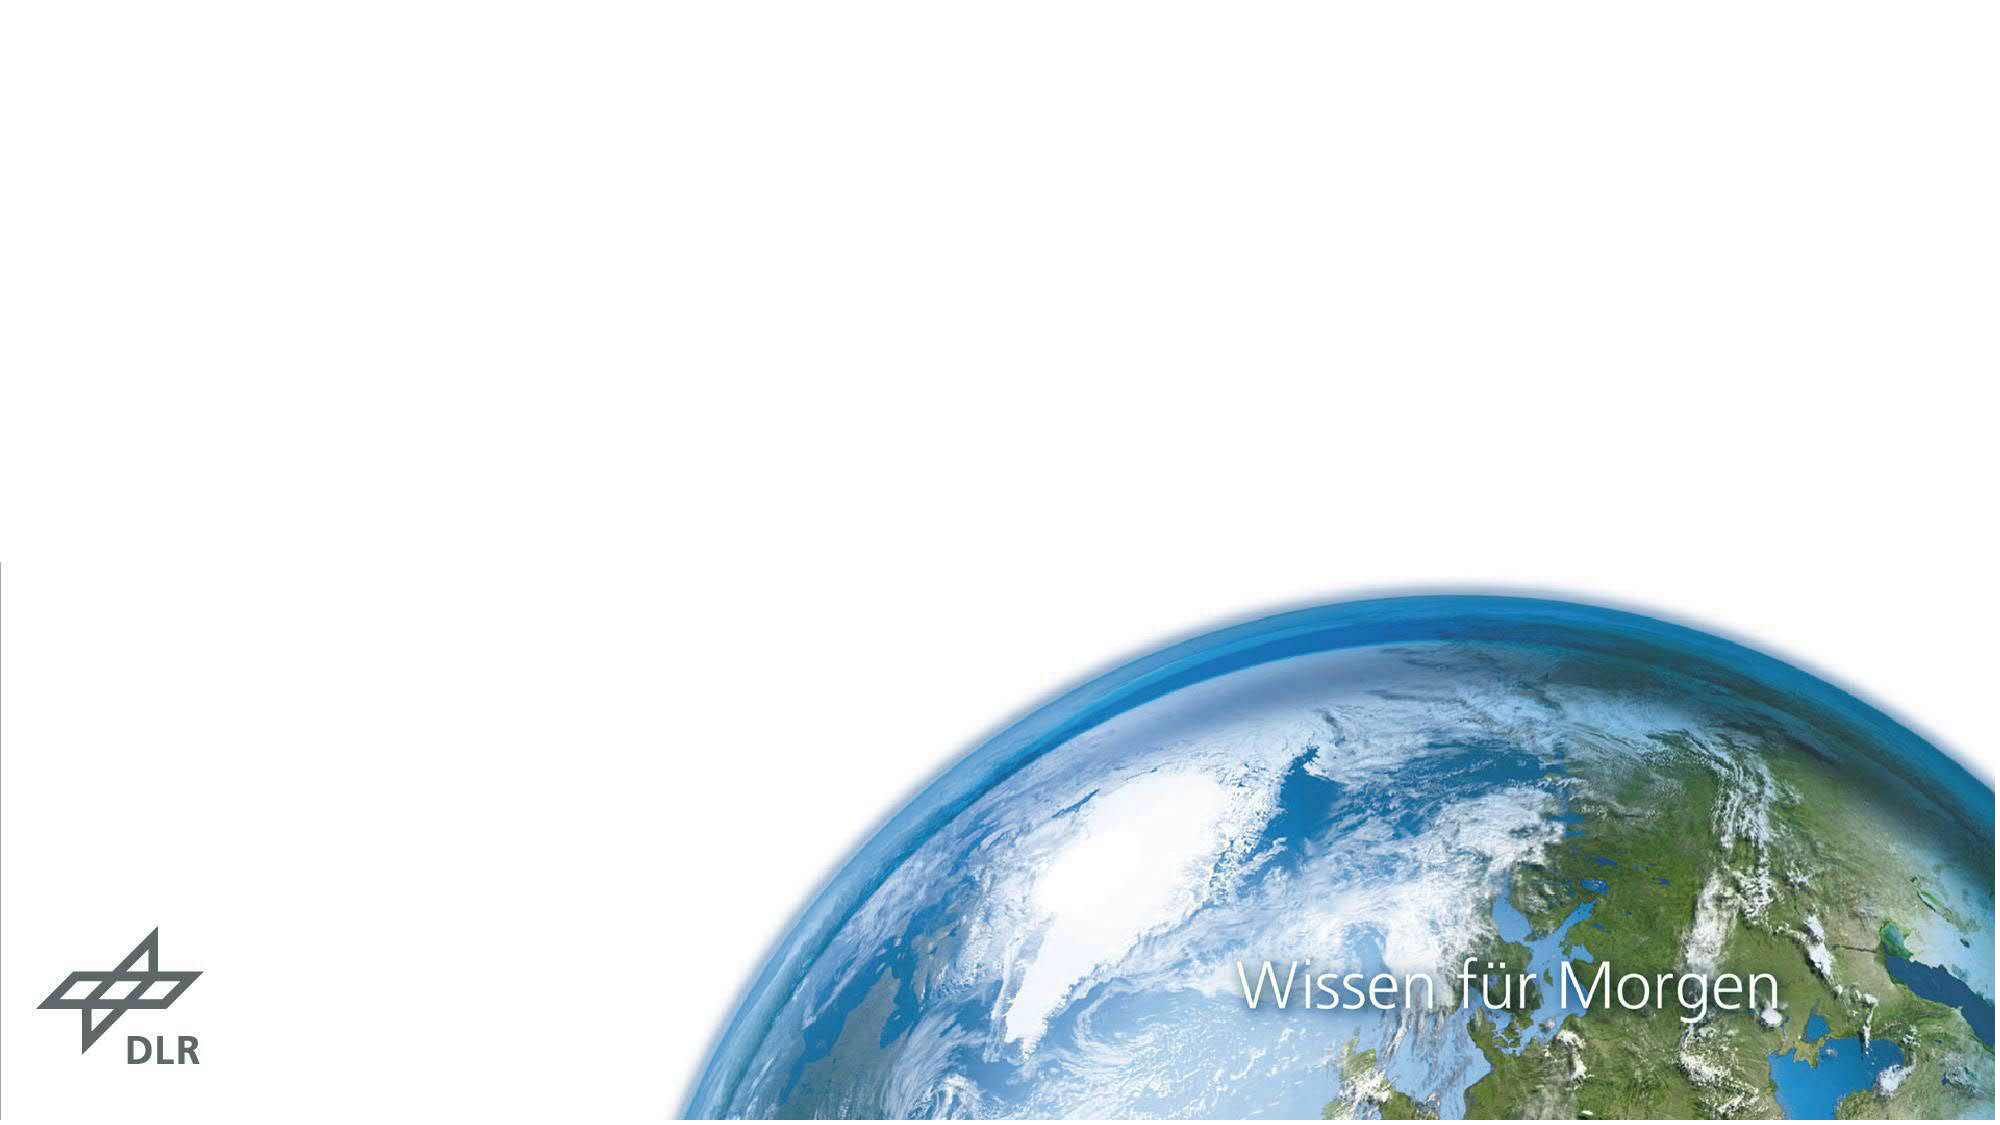
\includegraphics[page=1, width=\paperwidth]{header.pdf}};
		\node[text=mypres,anchor=south west,font=\sffamily\LARGE,text width=0.8\paperwidth] at ([xshift=7pt,yshift=1.50cm]current page.west) (title) {\raggedleft\insertshorttitle};
		\node[text=mypres,anchor=south west,font=\sffamily\large,text width=0.8\paperwidth] at ([xshift=7pt,yshift=1.00cm]current page.west) (subtitle) {\raggedleft\inserttitle};
		\node[text=mypres,anchor=south west,font=\sffamily,text width=.55\paperwidth] at ([xshift=7pt,yshift=-1cm]current page.west) (author) {\raggedright\insertauthor};
		\node[text=mypres,anchor=south west,font=\sffamily,text width=.55\paperwidth] at ([xshift=7pt,yshift=-1.5cm]current page.west) (date) {\raggedright\insertdate};
	\end{tikzpicture}
	\vskip0pt
}

% remove navigation symbols
\setbeamertemplate{navigation symbols}{}

\title[CoolingGen]{Eine Software zur Erstellung von Kühlungsgeometrien}
\author{Julian Lüken}
\date{\today}

\begin{document}

\begin{frame}[plain]
	\maketitle
\end{frame}

\begin{frame}
	\frametitle{Problemstellung / Kühlung}
	\vspace{-1cm}\hspace{-0.5cm}
	\centering
	\begin{minipage}[t]{0.8\textwidth}
		\centering
		\hspace{0.36\textwidth}
		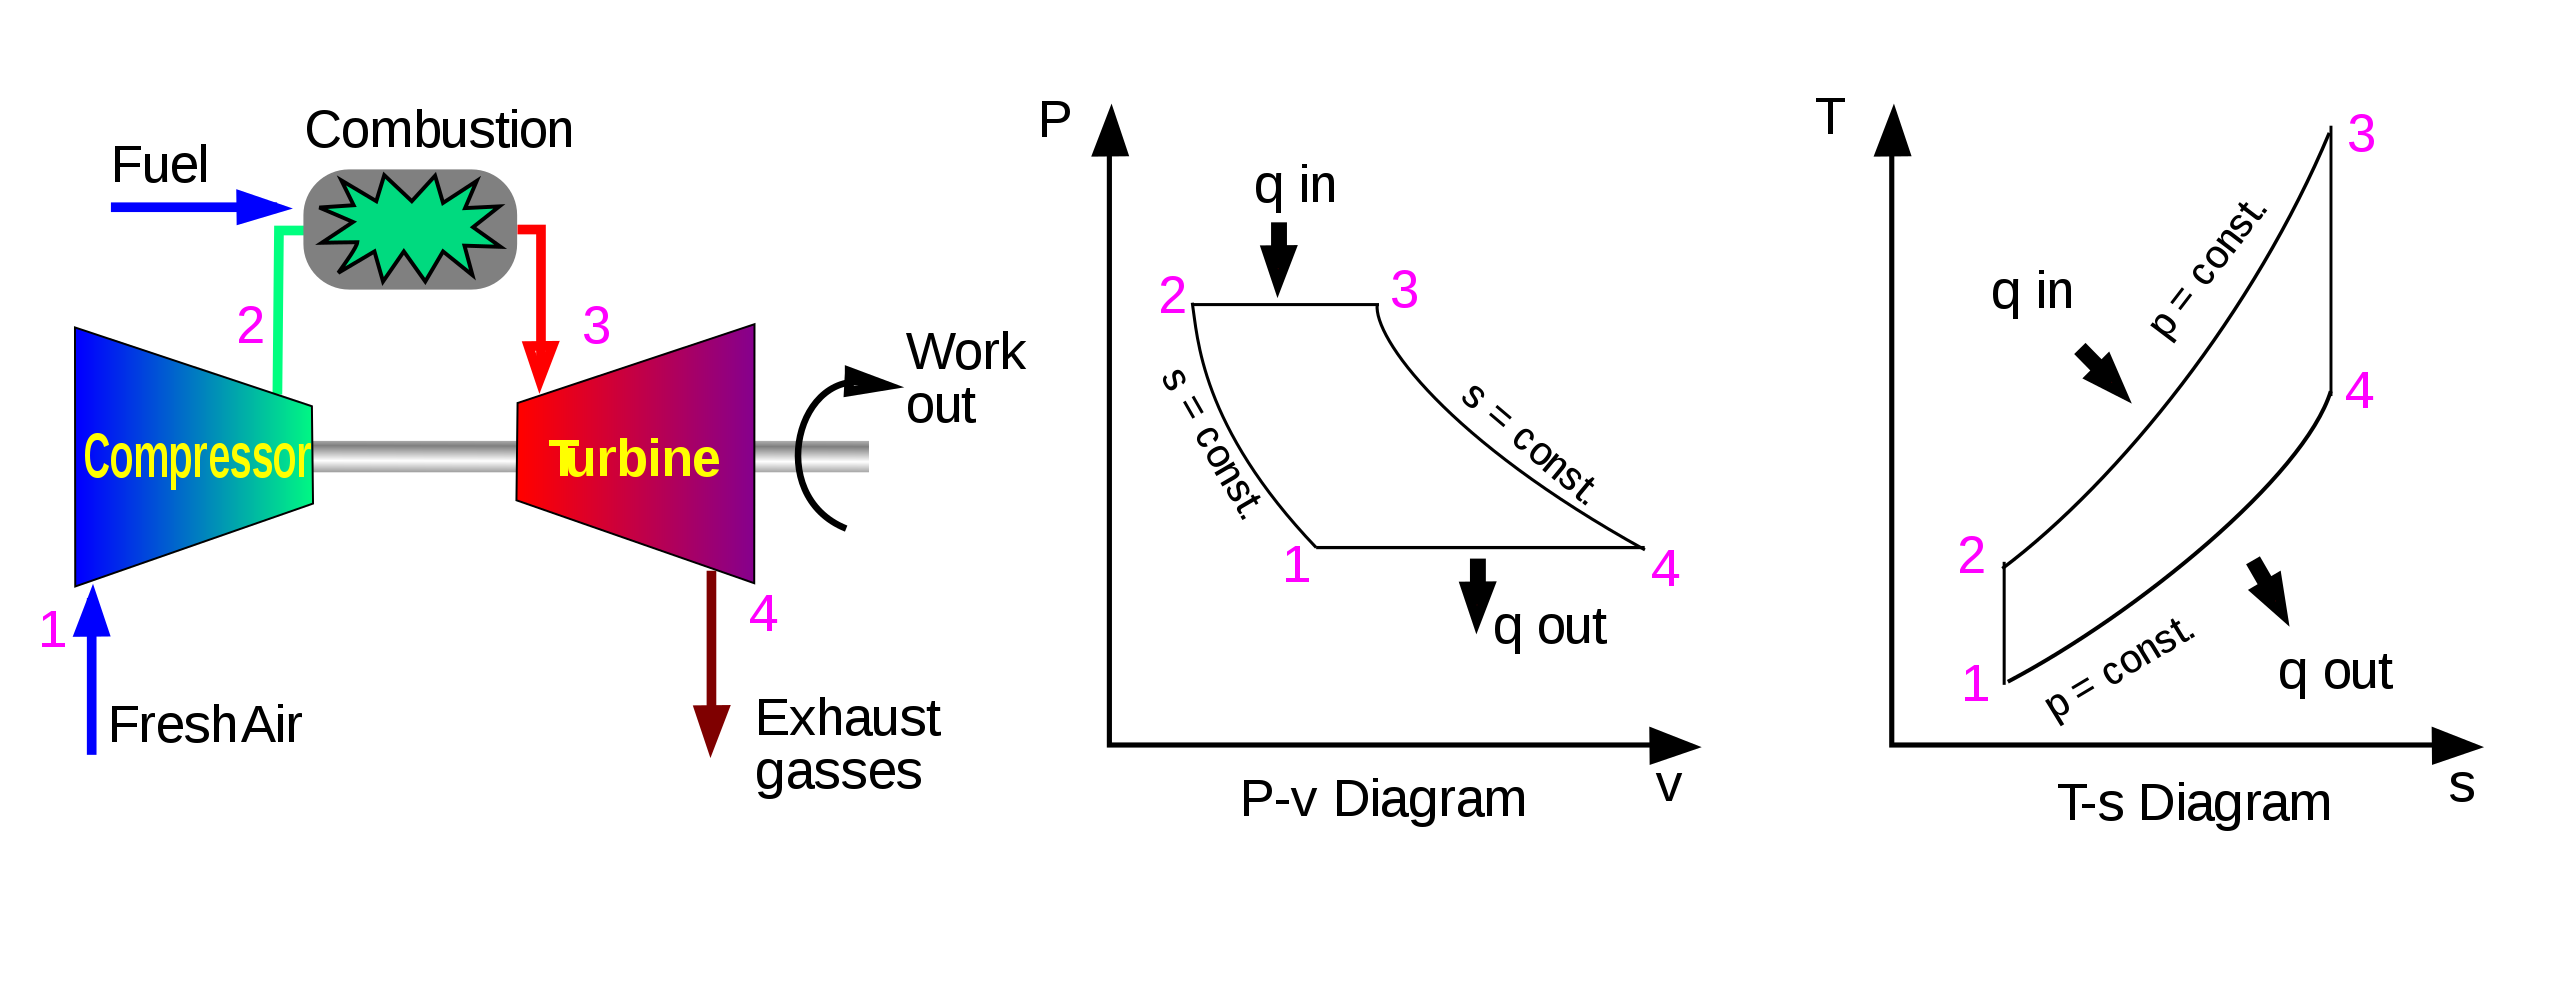
\includegraphics[width=0.625\textwidth]{images/Brayton_cycle.svg.png}
	\end{minipage}
	\begin{minipage}[t]{\textwidth}
		\begin{itemize}
			\item Effizienz der Turbine kann theoretisch durch großen Temperaturgradienten erhöht werden
			\item[] 	\textrightarrow{} Praktisch strebt man darum hohe Temperaturen in der Brennkammer an
			\item 		\textbf{Aber:} Hohe thermische Last der Turbinenschaufeln führt zu starker Abnutzung
			\item[] 	\textrightarrow{} Kühlung wird benötigt
			\item 		\textbf{Aber:} Die Kühlung wiederum nutzt Luftstrom, der nicht für den Antrieb benutzt werden kann
			\item[] 	\textrightarrow{} Negativer Einfluss auf Wirkungsgrad
			\item[] 	{}
			\item[\textrightarrow] \textbf{Kühlungsdesign ist Filigranarbeit!}
		\end{itemize}
	\end{minipage}
	\vfill
\end{frame}

\begin{frame}
	\frametitle{Problemstellung / Kühlung}
	\vspace{-1cm}\hspace{-0.5cm}
	\begin{minipage}[t]{0.5\textwidth}
		Kühlungsdesign setzt sich u.a. aus den folgenden Aspekten zusammen:
		\begin{itemize}
			\item Auswahl/Konditionierung der Kühlluft
			\item Auswahl der verwendeten Werkstoffe
			\item \textbf{Gestaltung der Kühlstrukturen}
		\end{itemize}
		\vspace{1em}
		Diese \textbf{Kühlstrukturen} beinhalten
		\begin{itemize}
			\item \textbf{Kühlkanäle} ("cooling channels"),
			\item \textbf{Prallkühlung} ("{}impingement cooling"),
			\item Rippen ("rib turbulators"),
			\item \textbf{Filmkühlung} ("film cooling"),
			\item \textbf{Pin-fins},
			\item und \textbf{Ausblasungsschlitze} ("trailing edge slots").
		\end{itemize}
	\end{minipage}
	\begin{minipage}[t]{0.48\textwidth}
			\begin{figure}[H]
			\centering
			\begin{subfigure}{.49\textwidth}
				\centering
				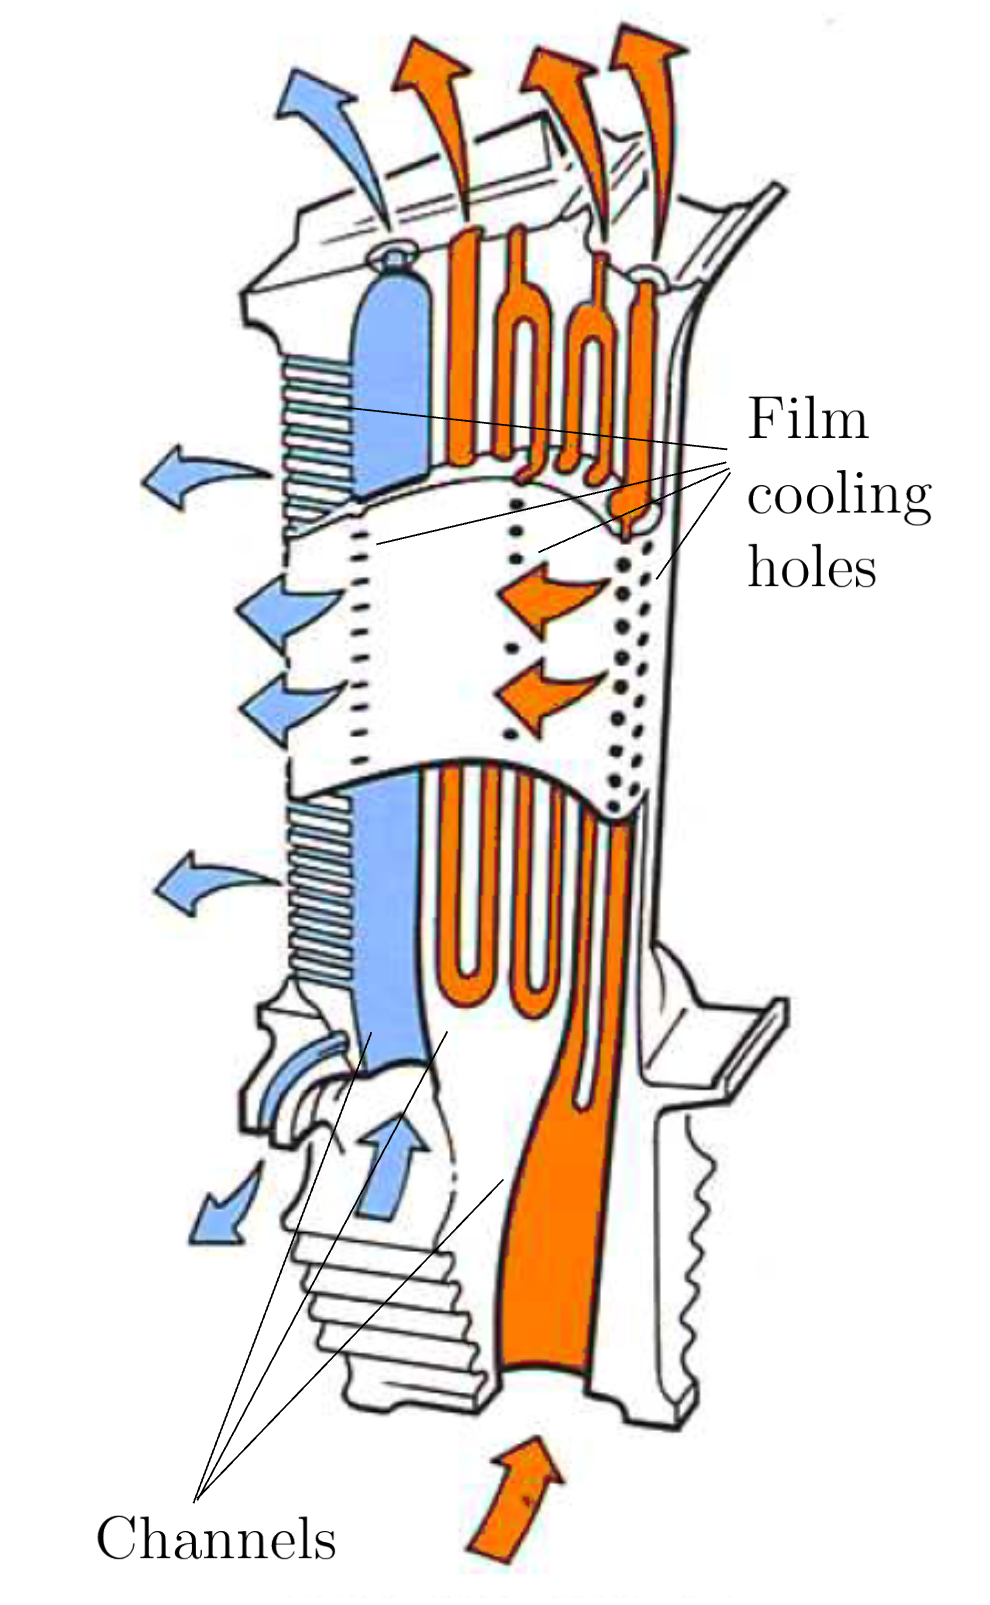
\includegraphics[width=.8\textwidth]{../../assets/rollsroyce/11.png}
				\caption{Rotor.}
			\end{subfigure}
			\begin{subfigure}{.49\textwidth}
				\centering
				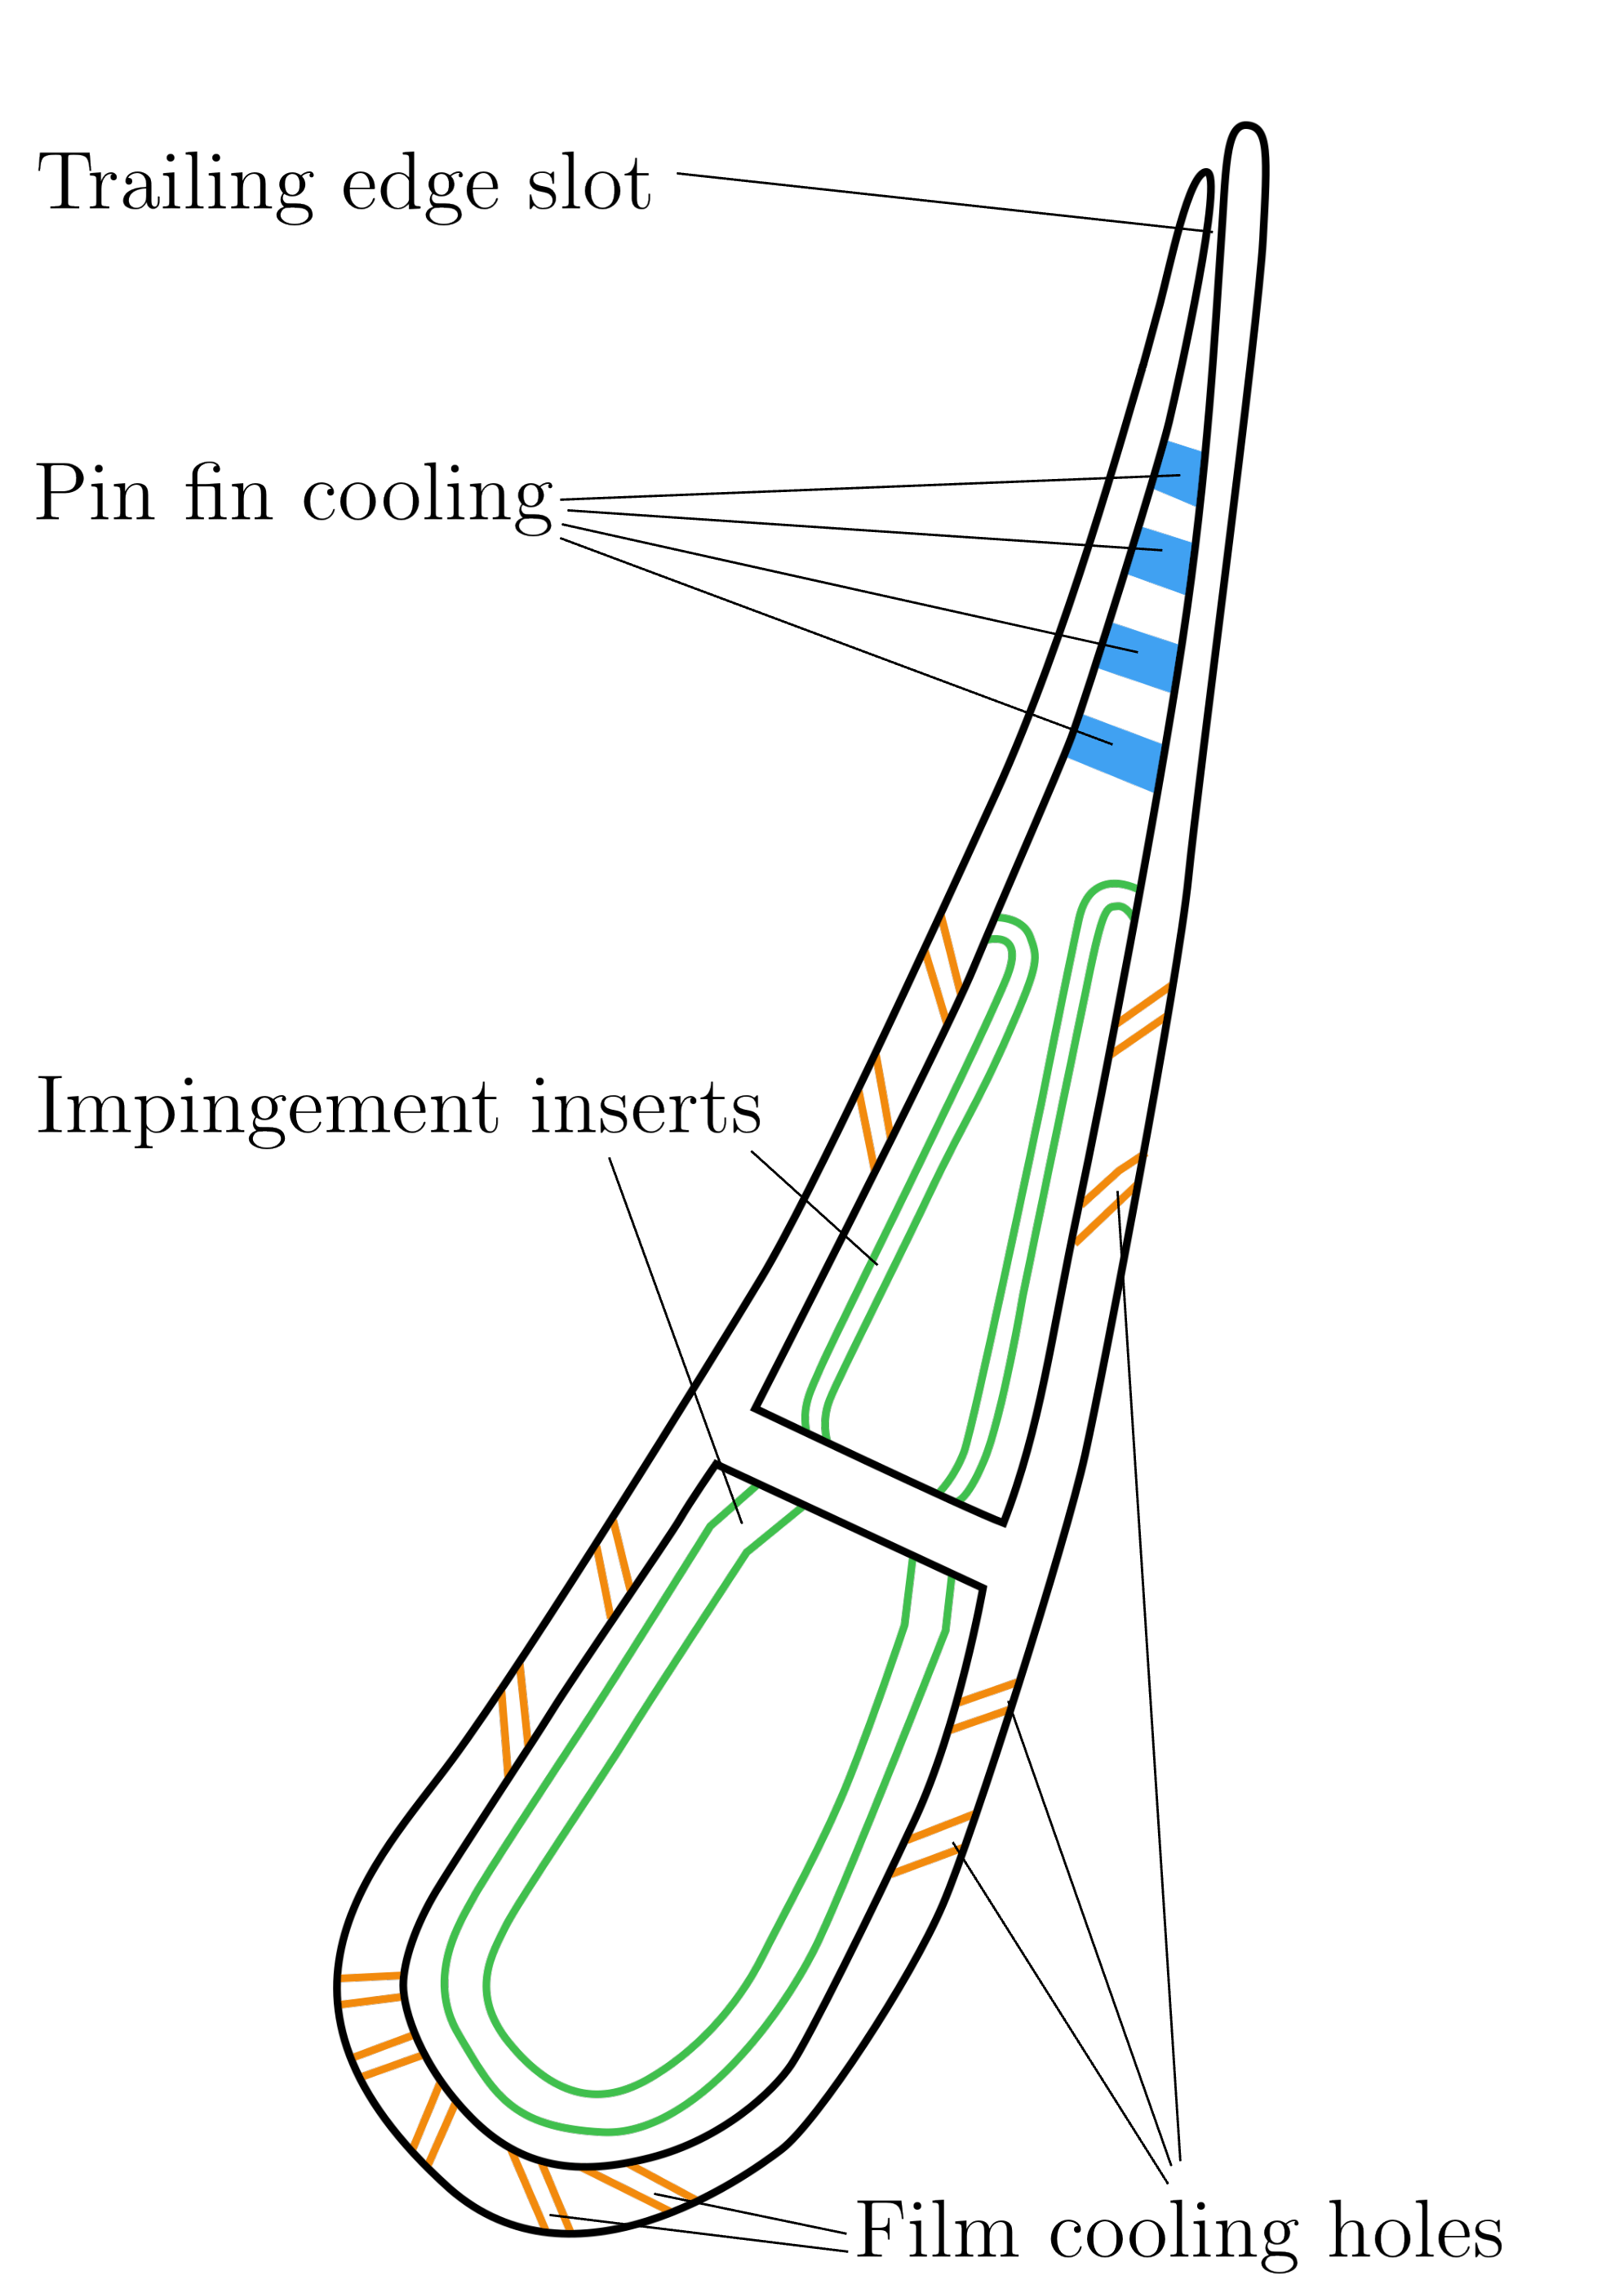
\includegraphics[width=.9\textwidth]{../../assets/gth_rebuild/11.png}
				\caption{Stator im Profil.}
			\end{subfigure}
		\end{figure}
	\end{minipage}
	\vfill
\end{frame}

\begin{frame}
	\frametitle{Problemstellung / Geometrieerzeugung}
	\vspace{-0.5cm}\hspace{-0.5cm}
	\begin{minipage}[t]{0.65\textwidth}
		\vspace{0.2cm}
		Mit CAD-Software lassen sich solche Strukturen erstellen. Leider ist der Prozess zeitaufwendig und schwierig.
		\begin{itemize}
			\item Parametrische Werkzeuge innerhalb herkömmlicher CAD Software bieten meistens nur eine semantische Schnittstelle für einfache Strukturen (z.B. Zylinder, Quader, Kegel), die sich allerdings beliebig miteinander kombinieren lassen (z.B. Verschneiden, Vereinen).
			\item Durch die Erstellung von Freiformkörpern gibt es gar keine parametrische Schnittstelle zur "mechanischen Realität". Dies beeinträchtigt die Möglichkeit zur einfachen Modifikation.
			\item[\textrightarrow] In beiden Fällen entsteht ein Modell, welches schwierig zu erstellen/modifizieren ist.
		\end{itemize}
		\vspace{1em}
		\textbf{Unser Lösungsansatz:} Wir erstellen uns eine eigene CAD-Software, die für uns die speziellen Kühlstrukturen mithilfe von bedeutungsträchtigen Parametern erstellt. Damit geht die Erstellung und Modifikation von Kühlungsgeometrien einfacher und schneller.
	\end{minipage}
	\begin{minipage}[t]{0.35\textwidth}
		\begin{figure}[H]
			\centering
			\begin{subfigure}{0.8\textwidth}
				\centering
				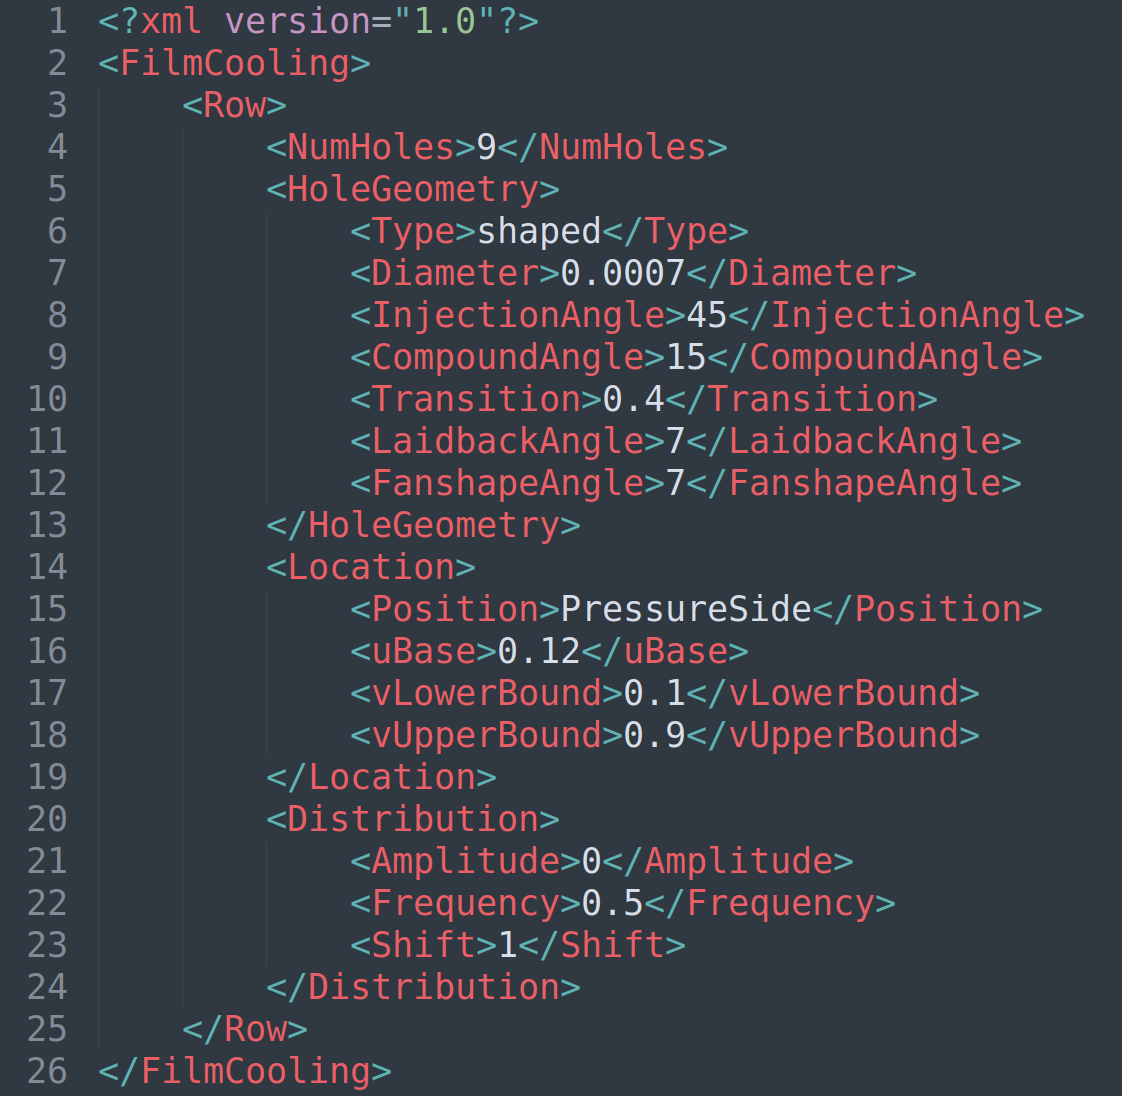
\includegraphics[width=\textwidth]{images/filmxml.png}
			\end{subfigure}\\
			$\Downarrow$\\
			\begin{subfigure}{0.8\textwidth}
				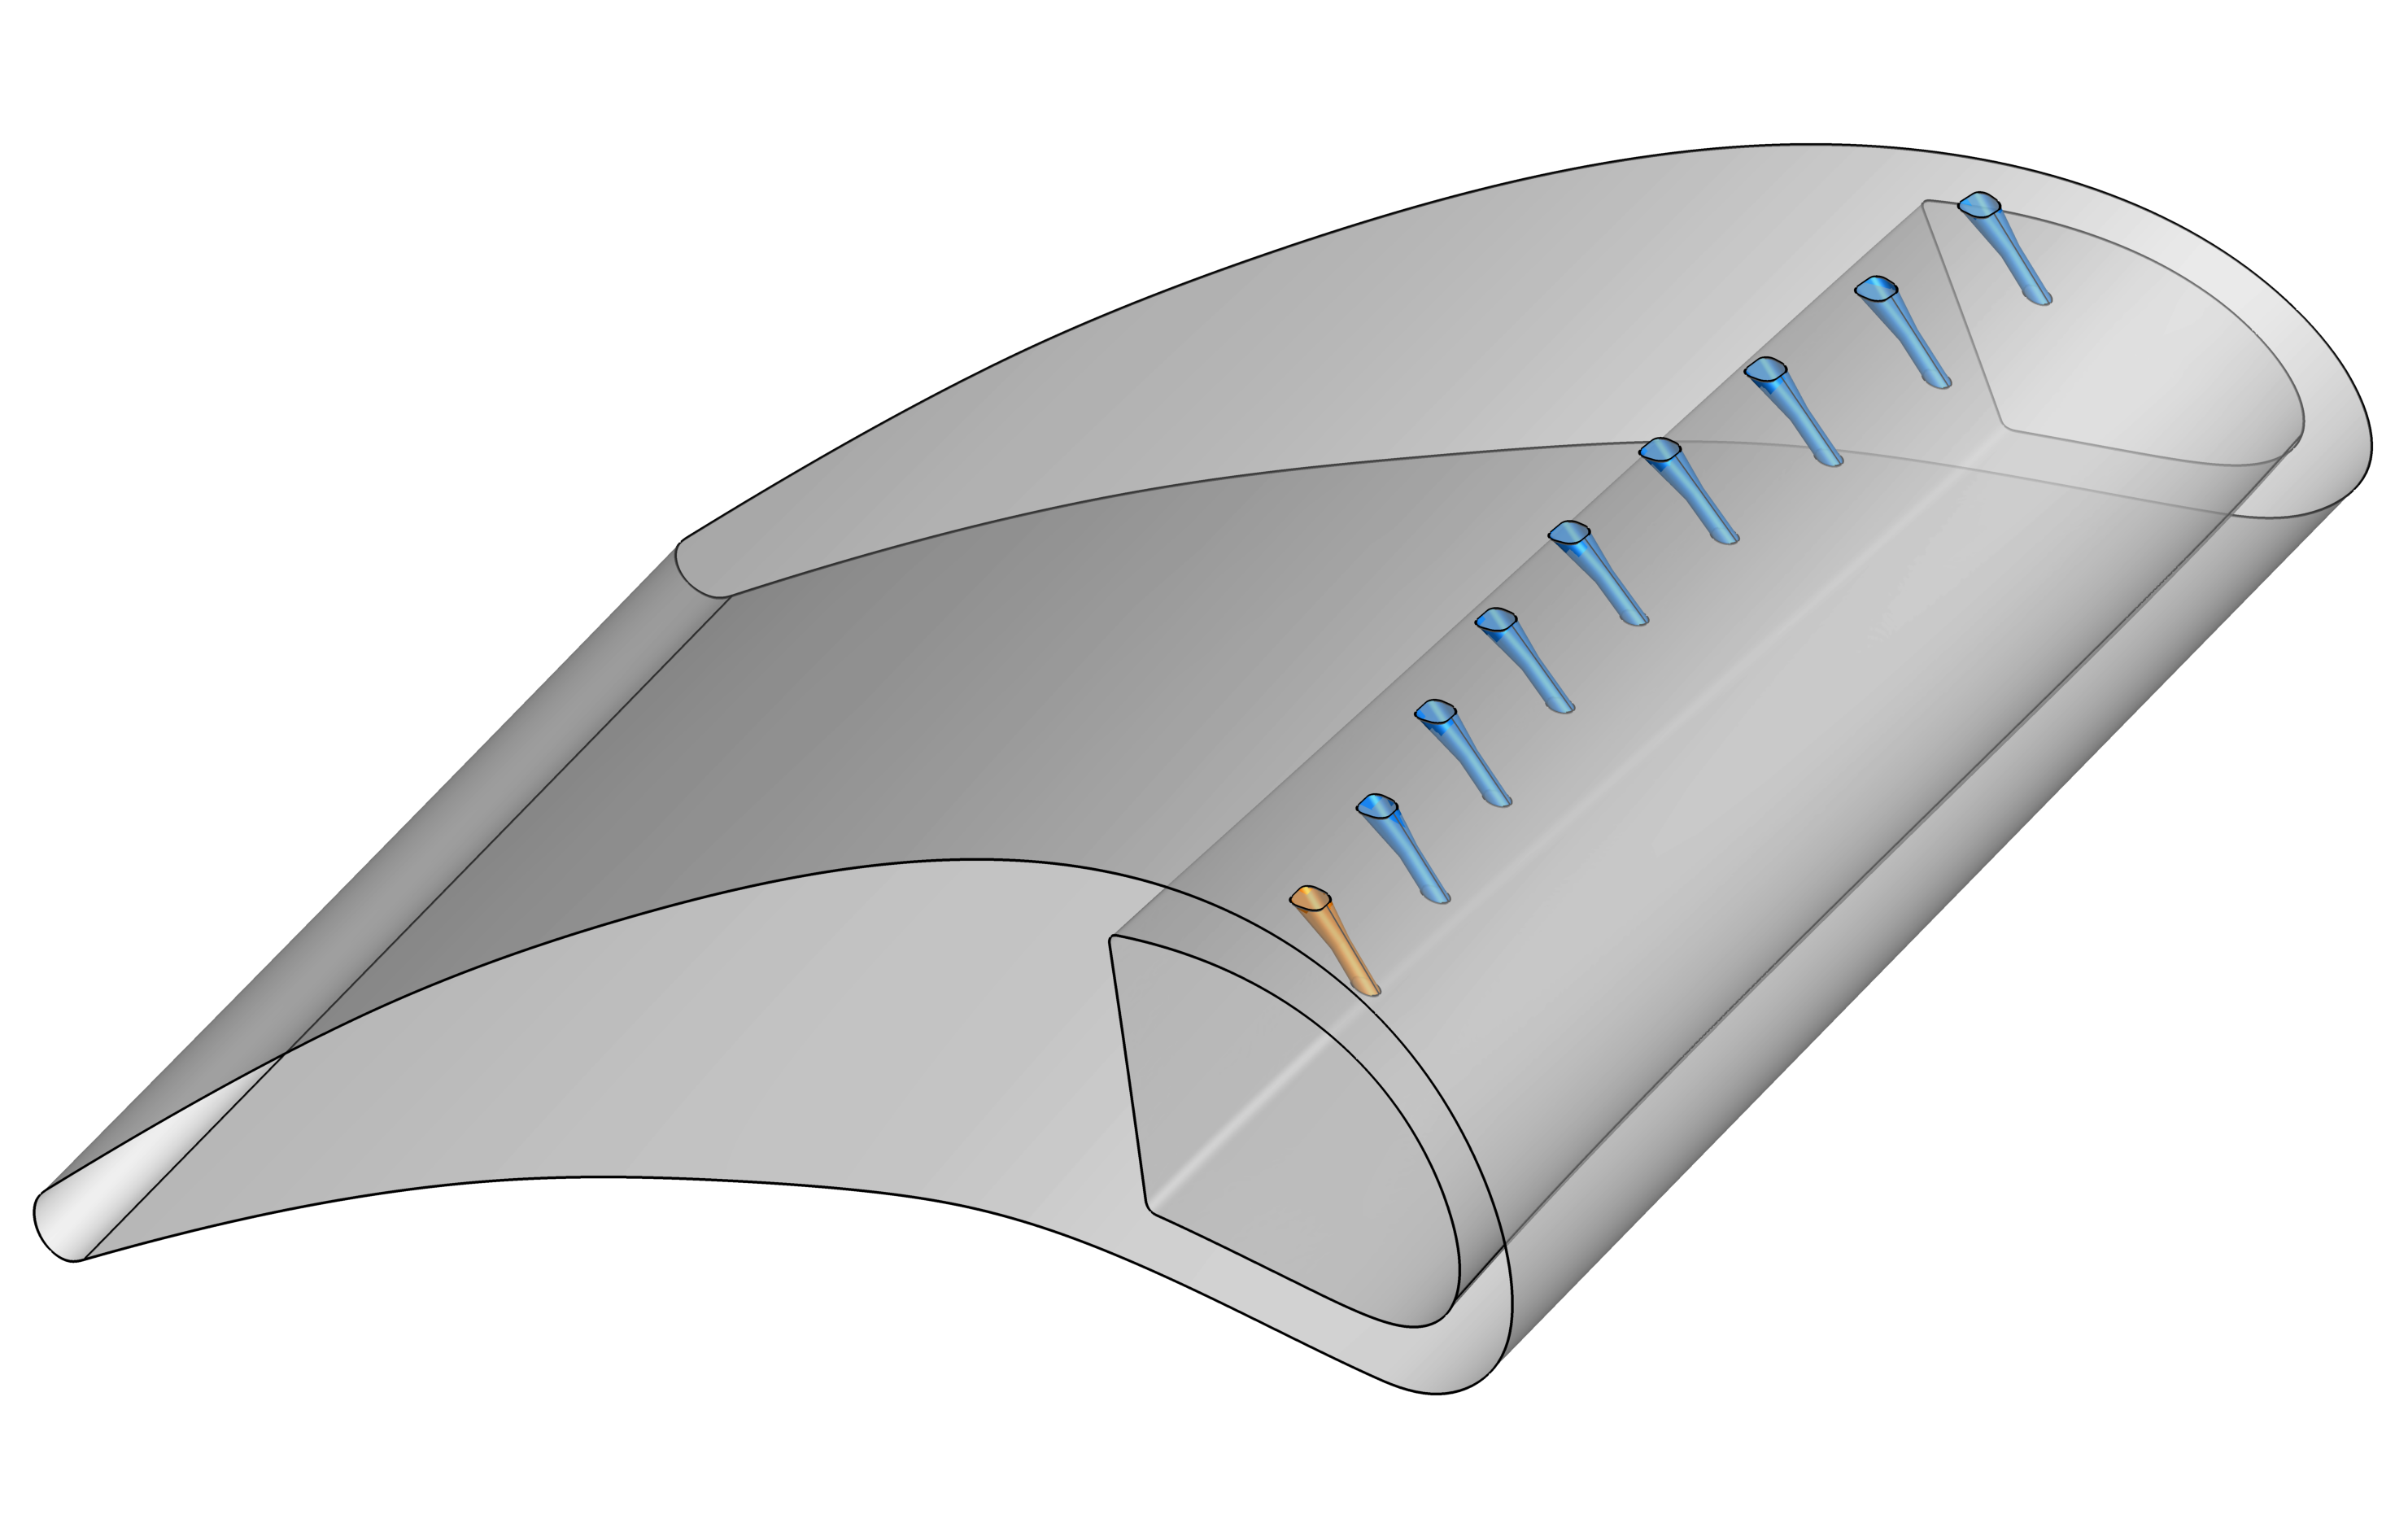
\includegraphics[width=\textwidth]{../../tec/holes/22edit.png}
			\end{subfigure}
		\end{figure}
	\end{minipage}
	\vfill
\end{frame}

\begin{frame}
	\frametitle{Geometrien / Überblick}
	\vspace{-1.5cm}\hspace{-0.5cm}
	\begin{minipage}[t]{0.38\textwidth}
		\begin{itemize}
			\item[\ding{109}] Kühlkanäle
			\item[\ding{109}] Filmkühlung
			\item[\ding{109}] Prallkühlung
			\item[\ding{109}] Ausblasungsschlitze
			\item[\ding{109}] Pin-fins
		\end{itemize}
	\end{minipage}
	\begin{minipage}{0.6\textwidth}
		\begin{figure}[H]
			\centering
			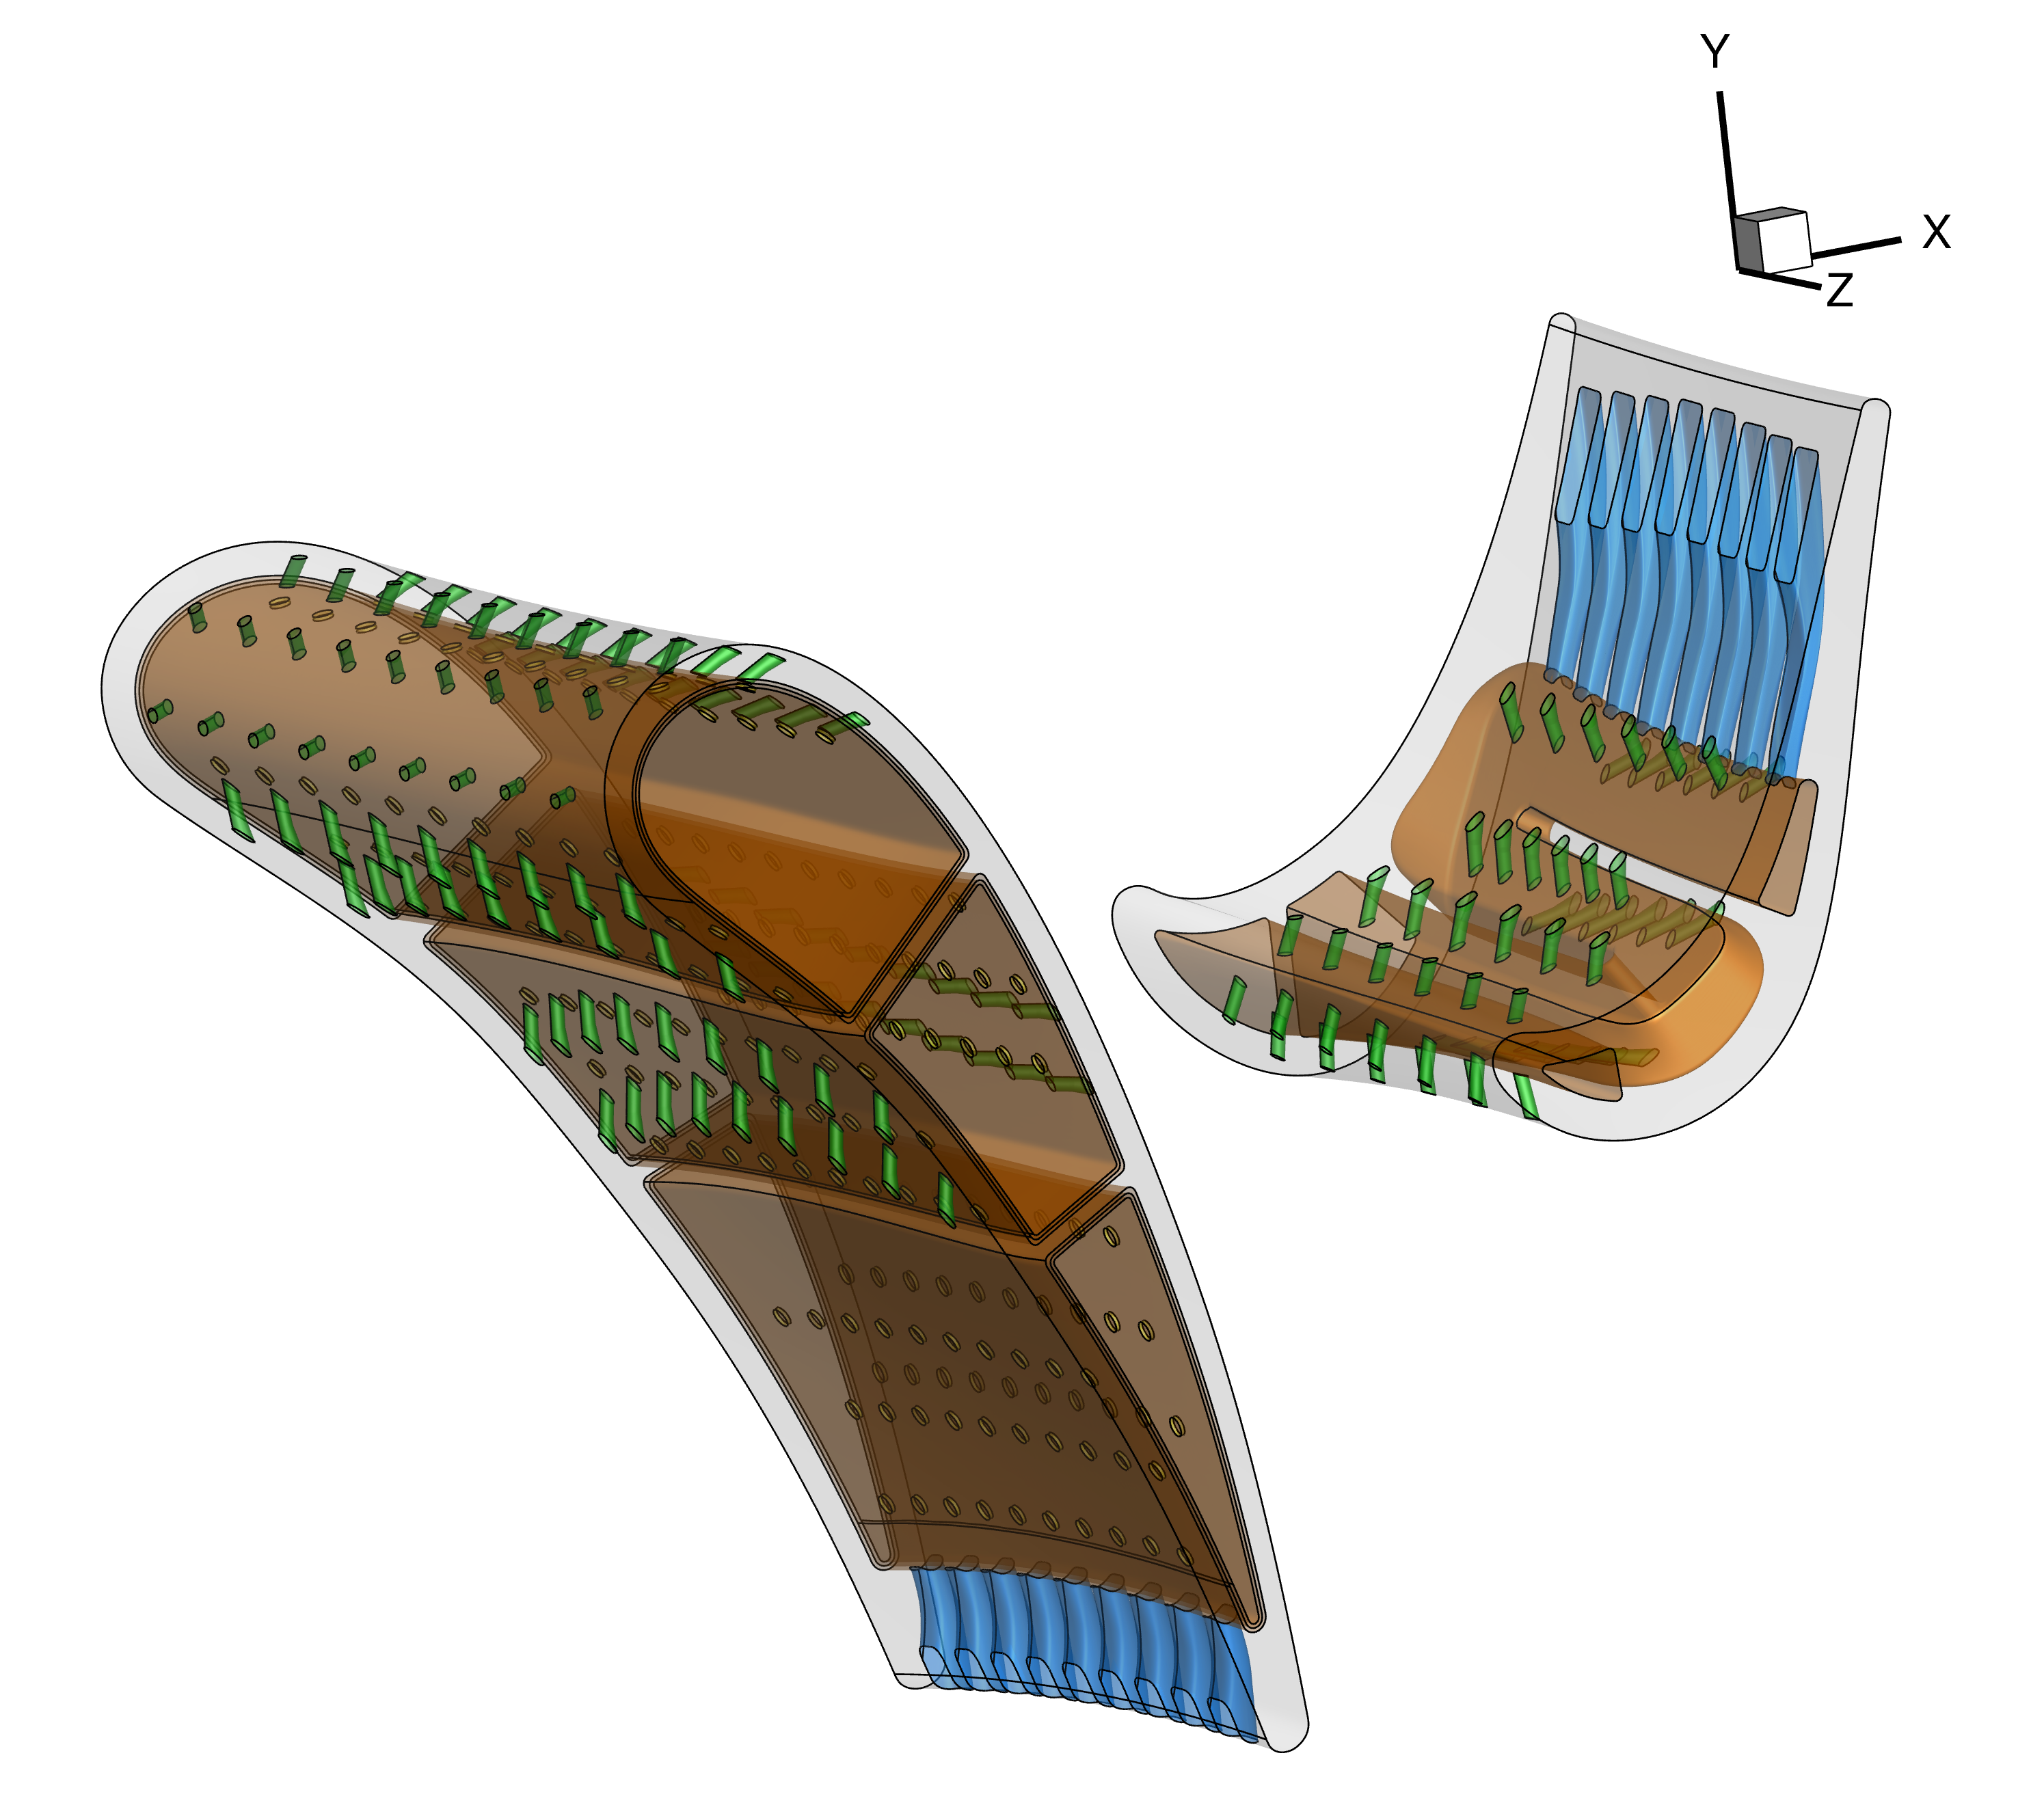
\includegraphics[width=\textwidth]{../../tec/complete/60.png}
		\end{figure}
	\end{minipage}
	\vfill
\end{frame}

\begin{frame}
	\frametitle{Geometrien / Überblick}
	\vspace{-1.5cm}\hspace{-0.5cm}
	\begin{minipage}[t]{0.38\textwidth}
		\begin{itemize}
			\item[\ding{40}] Kühlkanäle
			\item[\ding{109}] Filmkühlung
			\item[\ding{109}] Prallkühlung
			\item[\ding{109}] Ausblasungsschlitze
			\item[\ding{109}] Pin-fins
		\end{itemize}
	\end{minipage}
	\begin{minipage}{0.6\textwidth}
		\begin{figure}[H]
			\centering
			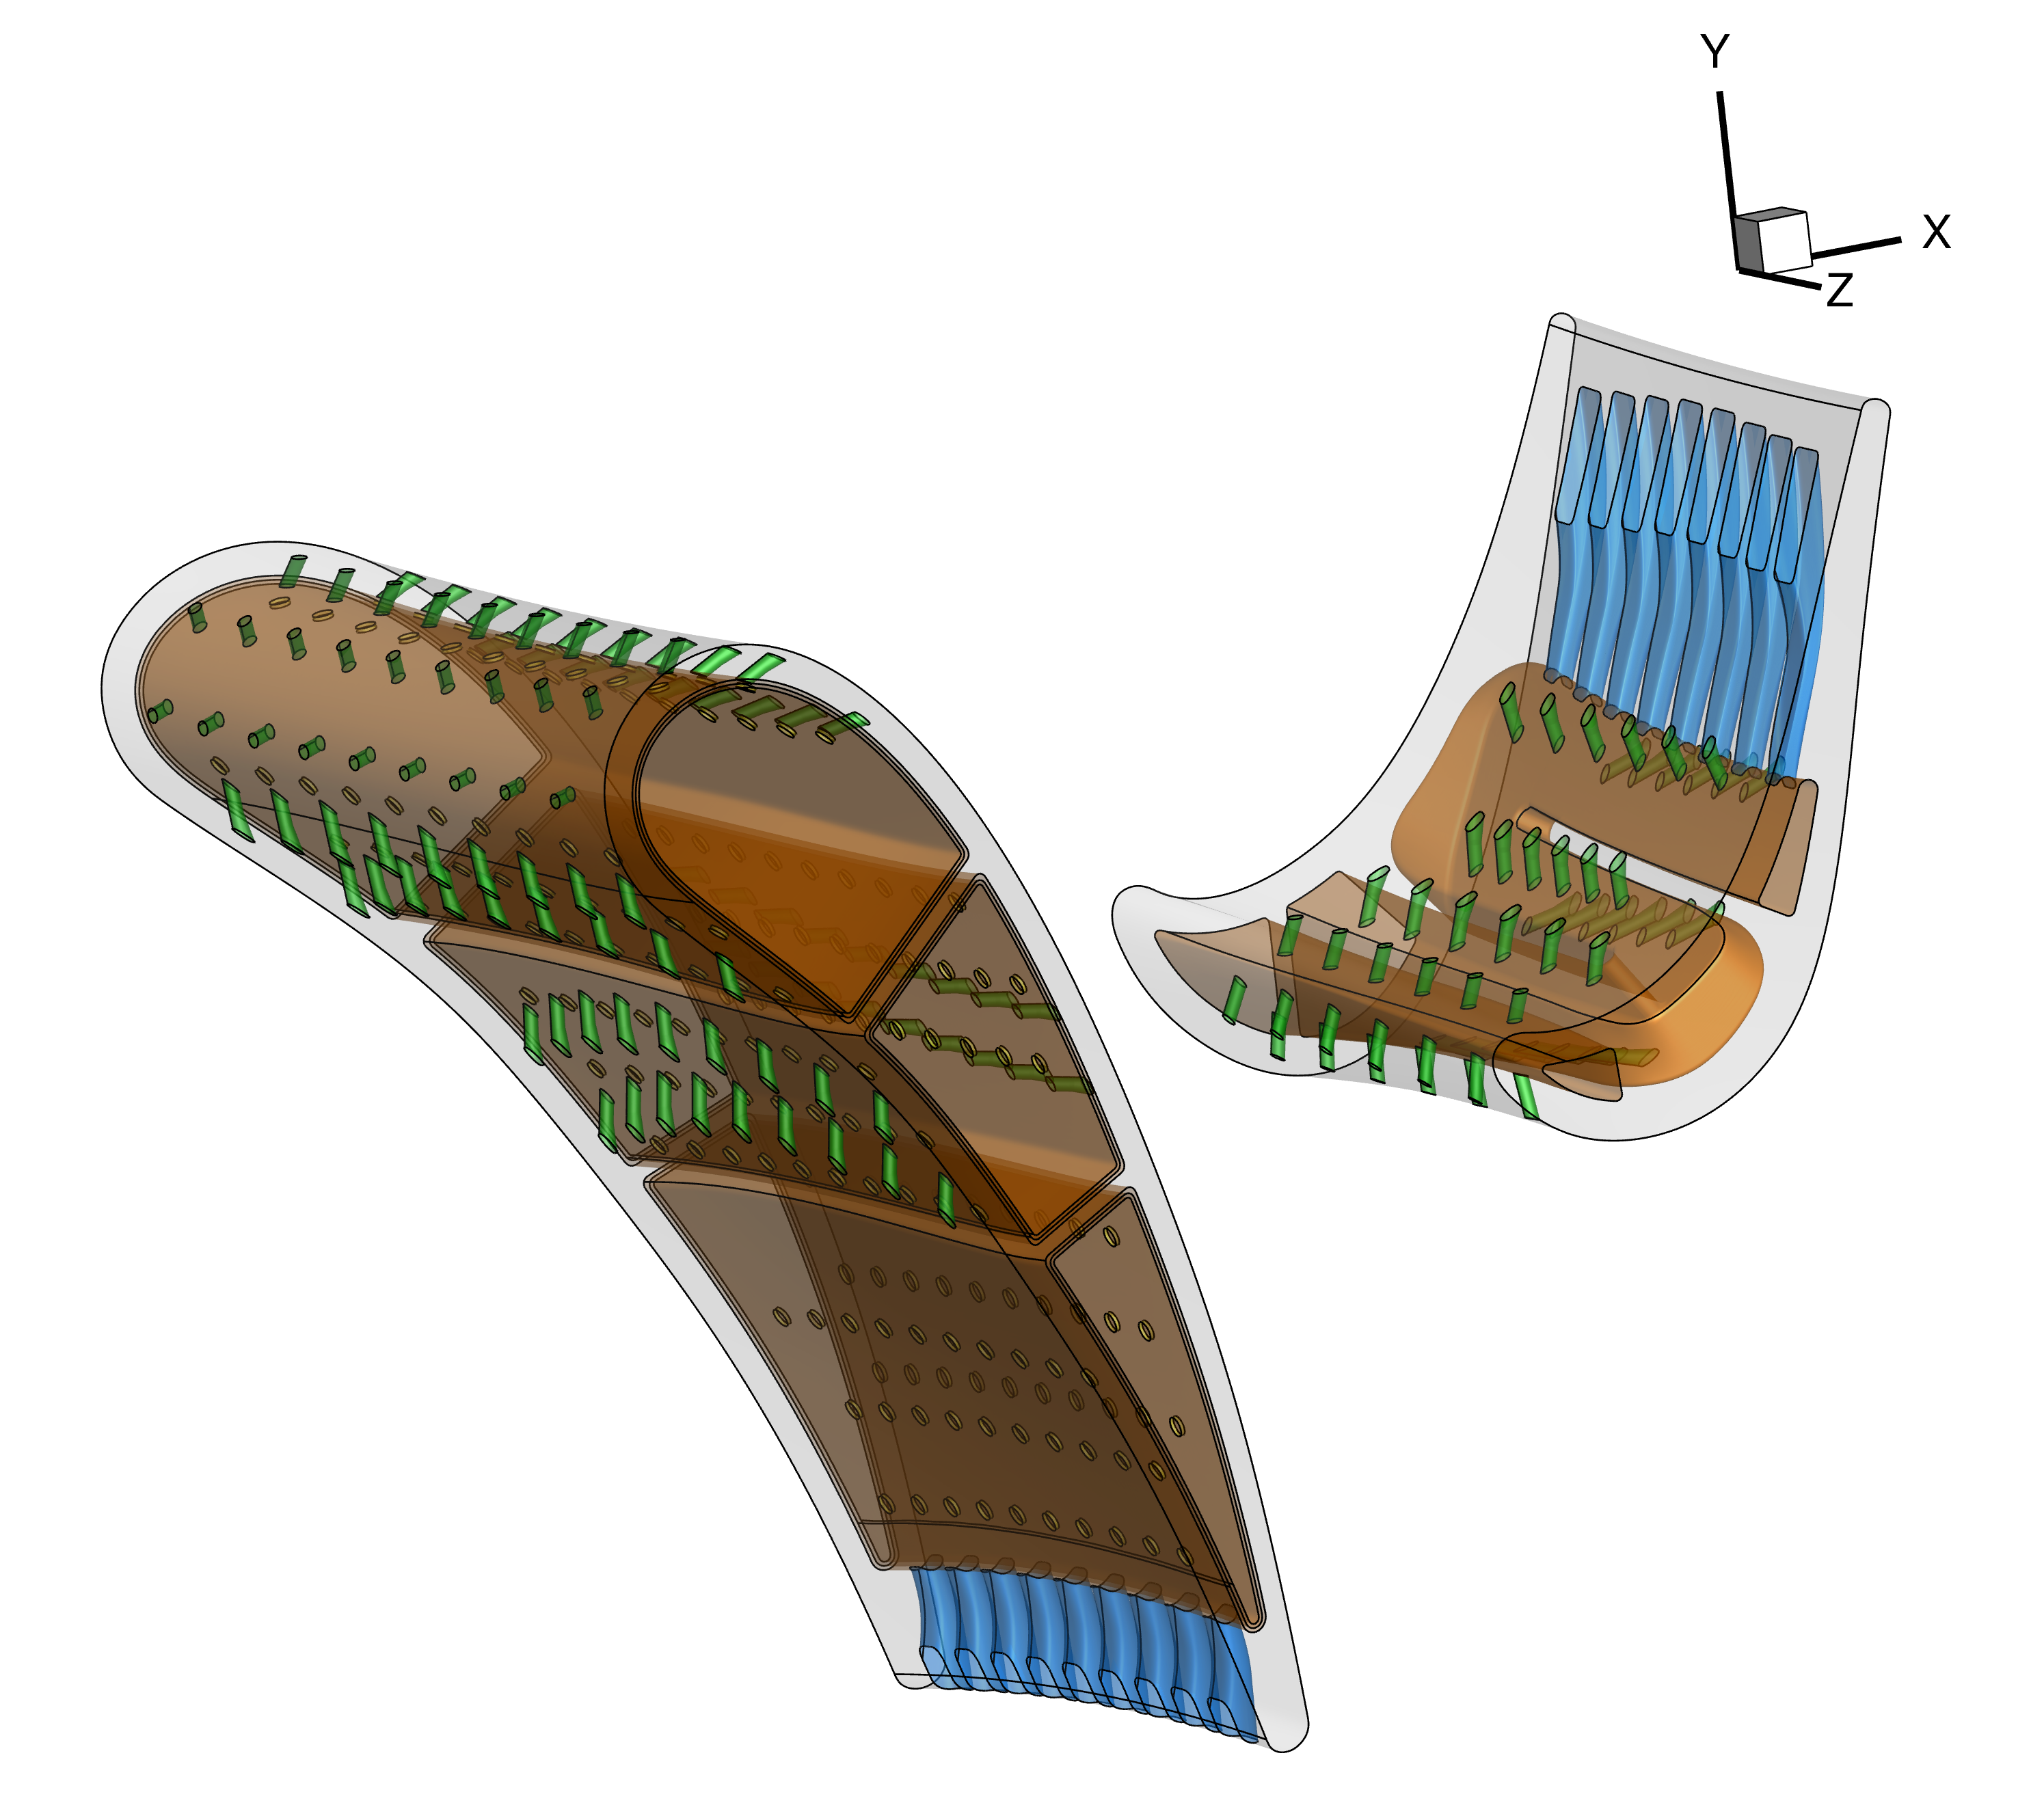
\includegraphics[width=\textwidth]{../../tec/complete/60.png}
		\end{figure}
	\end{minipage}
	\vfill
\end{frame}

\begin{frame}
	\frametitle{Geometrien / Kanäle}
	\vspace{-0.25cm}\hspace{-0.5cm}
	\begin{minipage}[t]{\textwidth}
		Bei der Erstellung von \textbf{Kühlkanälen} unterscheiden wir in CoolingGen zwischen zwei Teilstrukturen:\\[-.8em]

		\textbf{1. Kammern}\\
		Kammern ermöglichen dem Fluid, die Schaufel in radialer Richtung zu durchqueren (orange)\\[-.8em]
		
		\textbf{2. Umkehrungen}\\
		Umkehrungen ermöglichen den Transport des Fluids von einer Kammer in die nächste (blau)\\[-.8em]
	\end{minipage}
	\centering
	\begin{minipage}[t]{.8\textwidth}
		\begin{figure}[H]
			\centering
			\begin{subfigure}{.49\textwidth}
				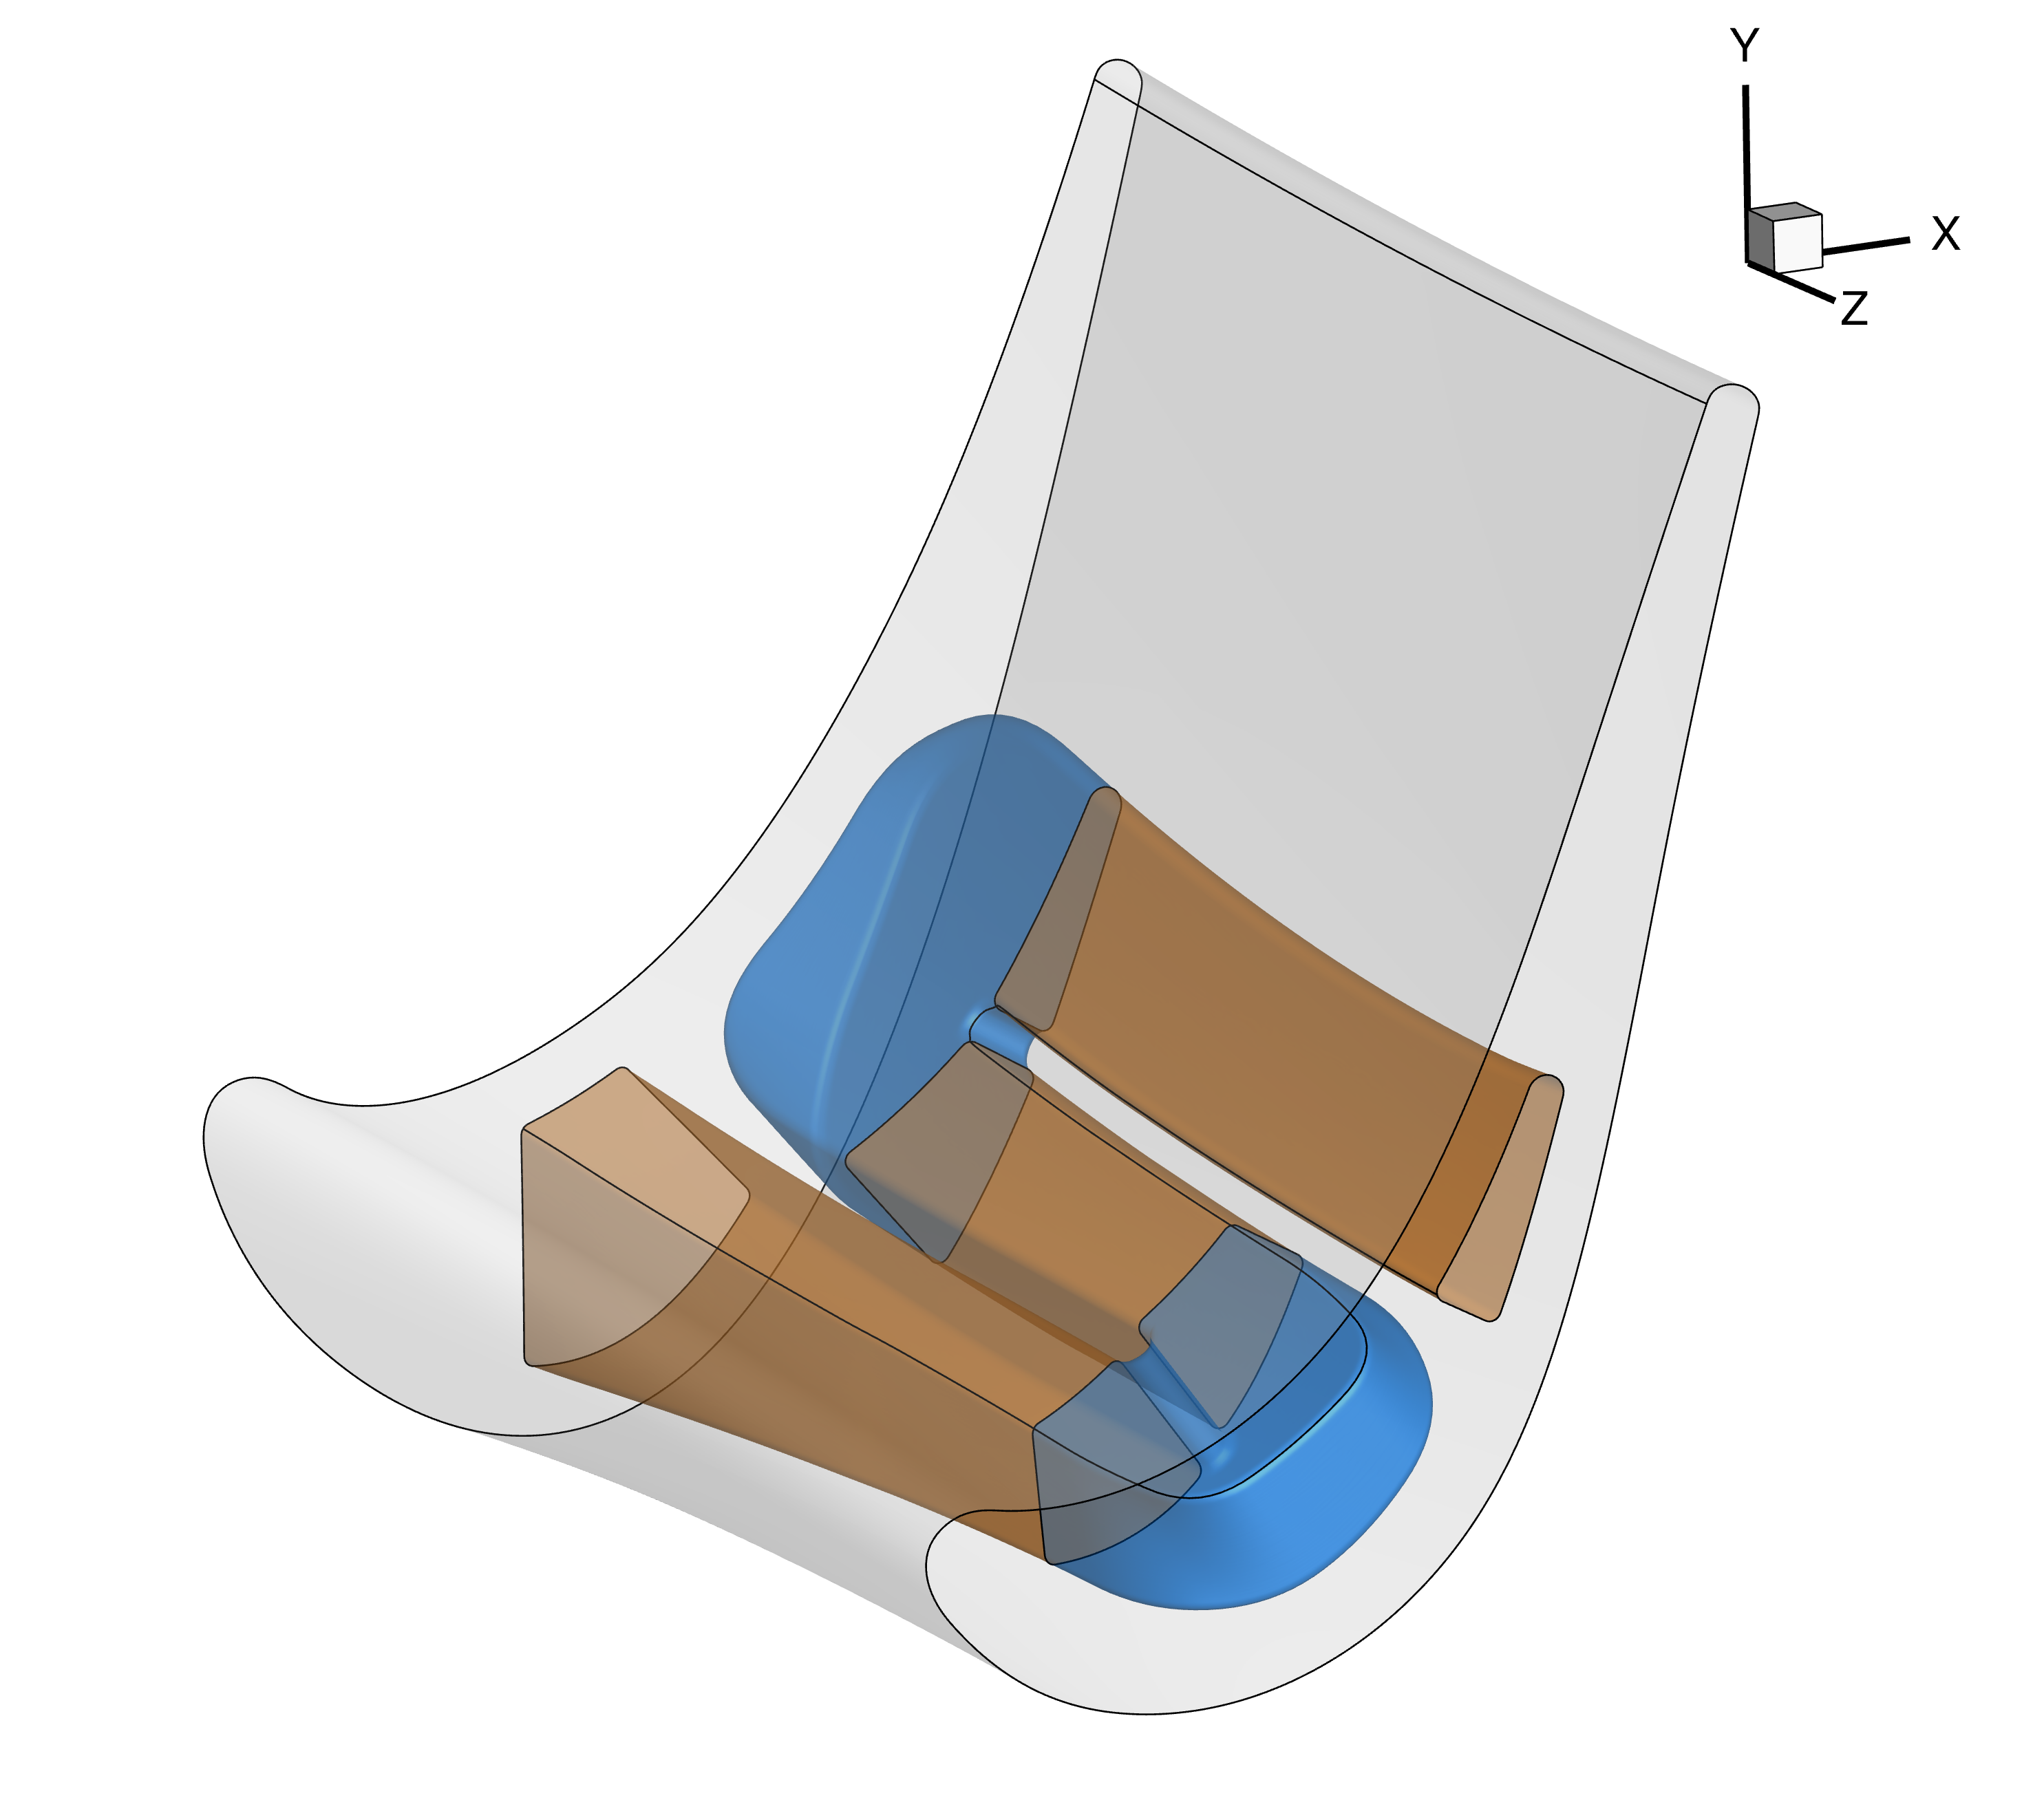
\includegraphics[width=\textwidth]{../../tec/complete/020.png}
			\end{subfigure}
			\begin{subfigure}{.49\textwidth}
				\centering
				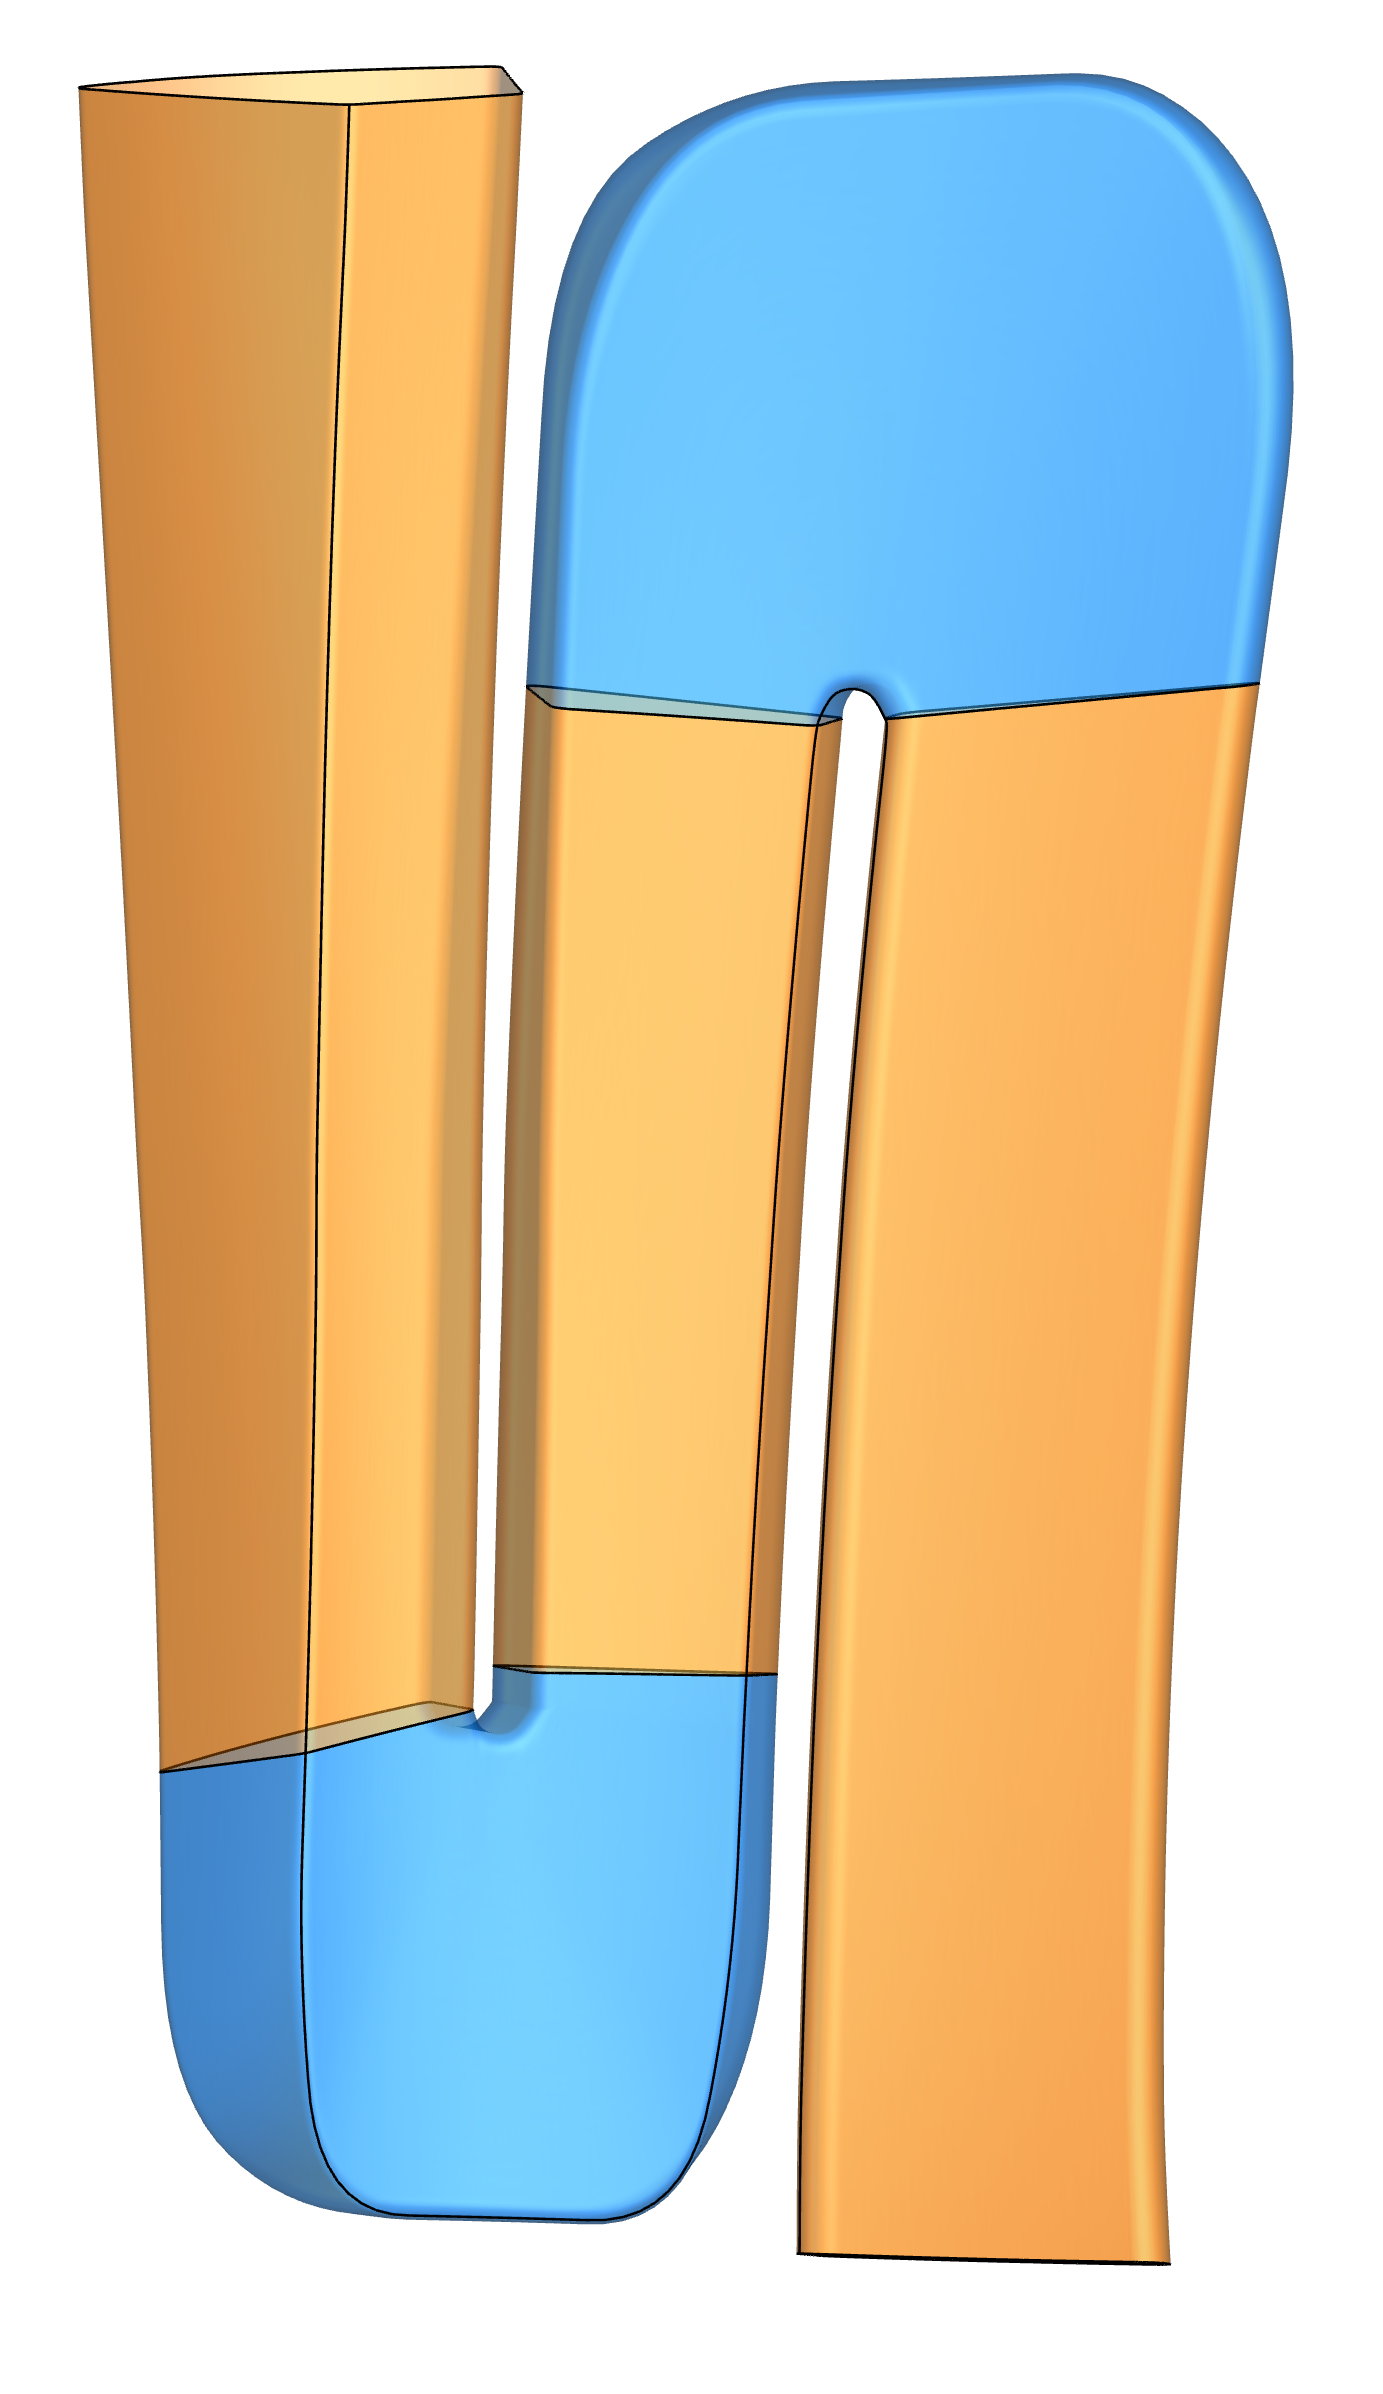
\includegraphics[width=.5\textwidth]{../../tec/complete/021.png}
			\end{subfigure}
		\end{figure}
	\end{minipage}
	\vfill
\end{frame}

\begin{frame}
	\frametitle{Geometrien / Kanäle / Kammern}
	\vspace{-0.25cm}\hspace{-0.5cm}
	\centering
	\begin{minipage}[t]{\textwidth}
		Zum Erstellen der Kammern begeben wir uns vom Standardkoordinatensystem $(x,y,z)$ in das $(m, r\theta)$ \textbf{Stromlinien-Koordinatensystem}. Hier sind die isoradialen Profilkurven der Schaufeln auf kanonische Weise 2D, was viele Operationen vereinfacht.
		\begin{figure}[H]
			\centering
			\begin{subfigure}{.32\textwidth}
				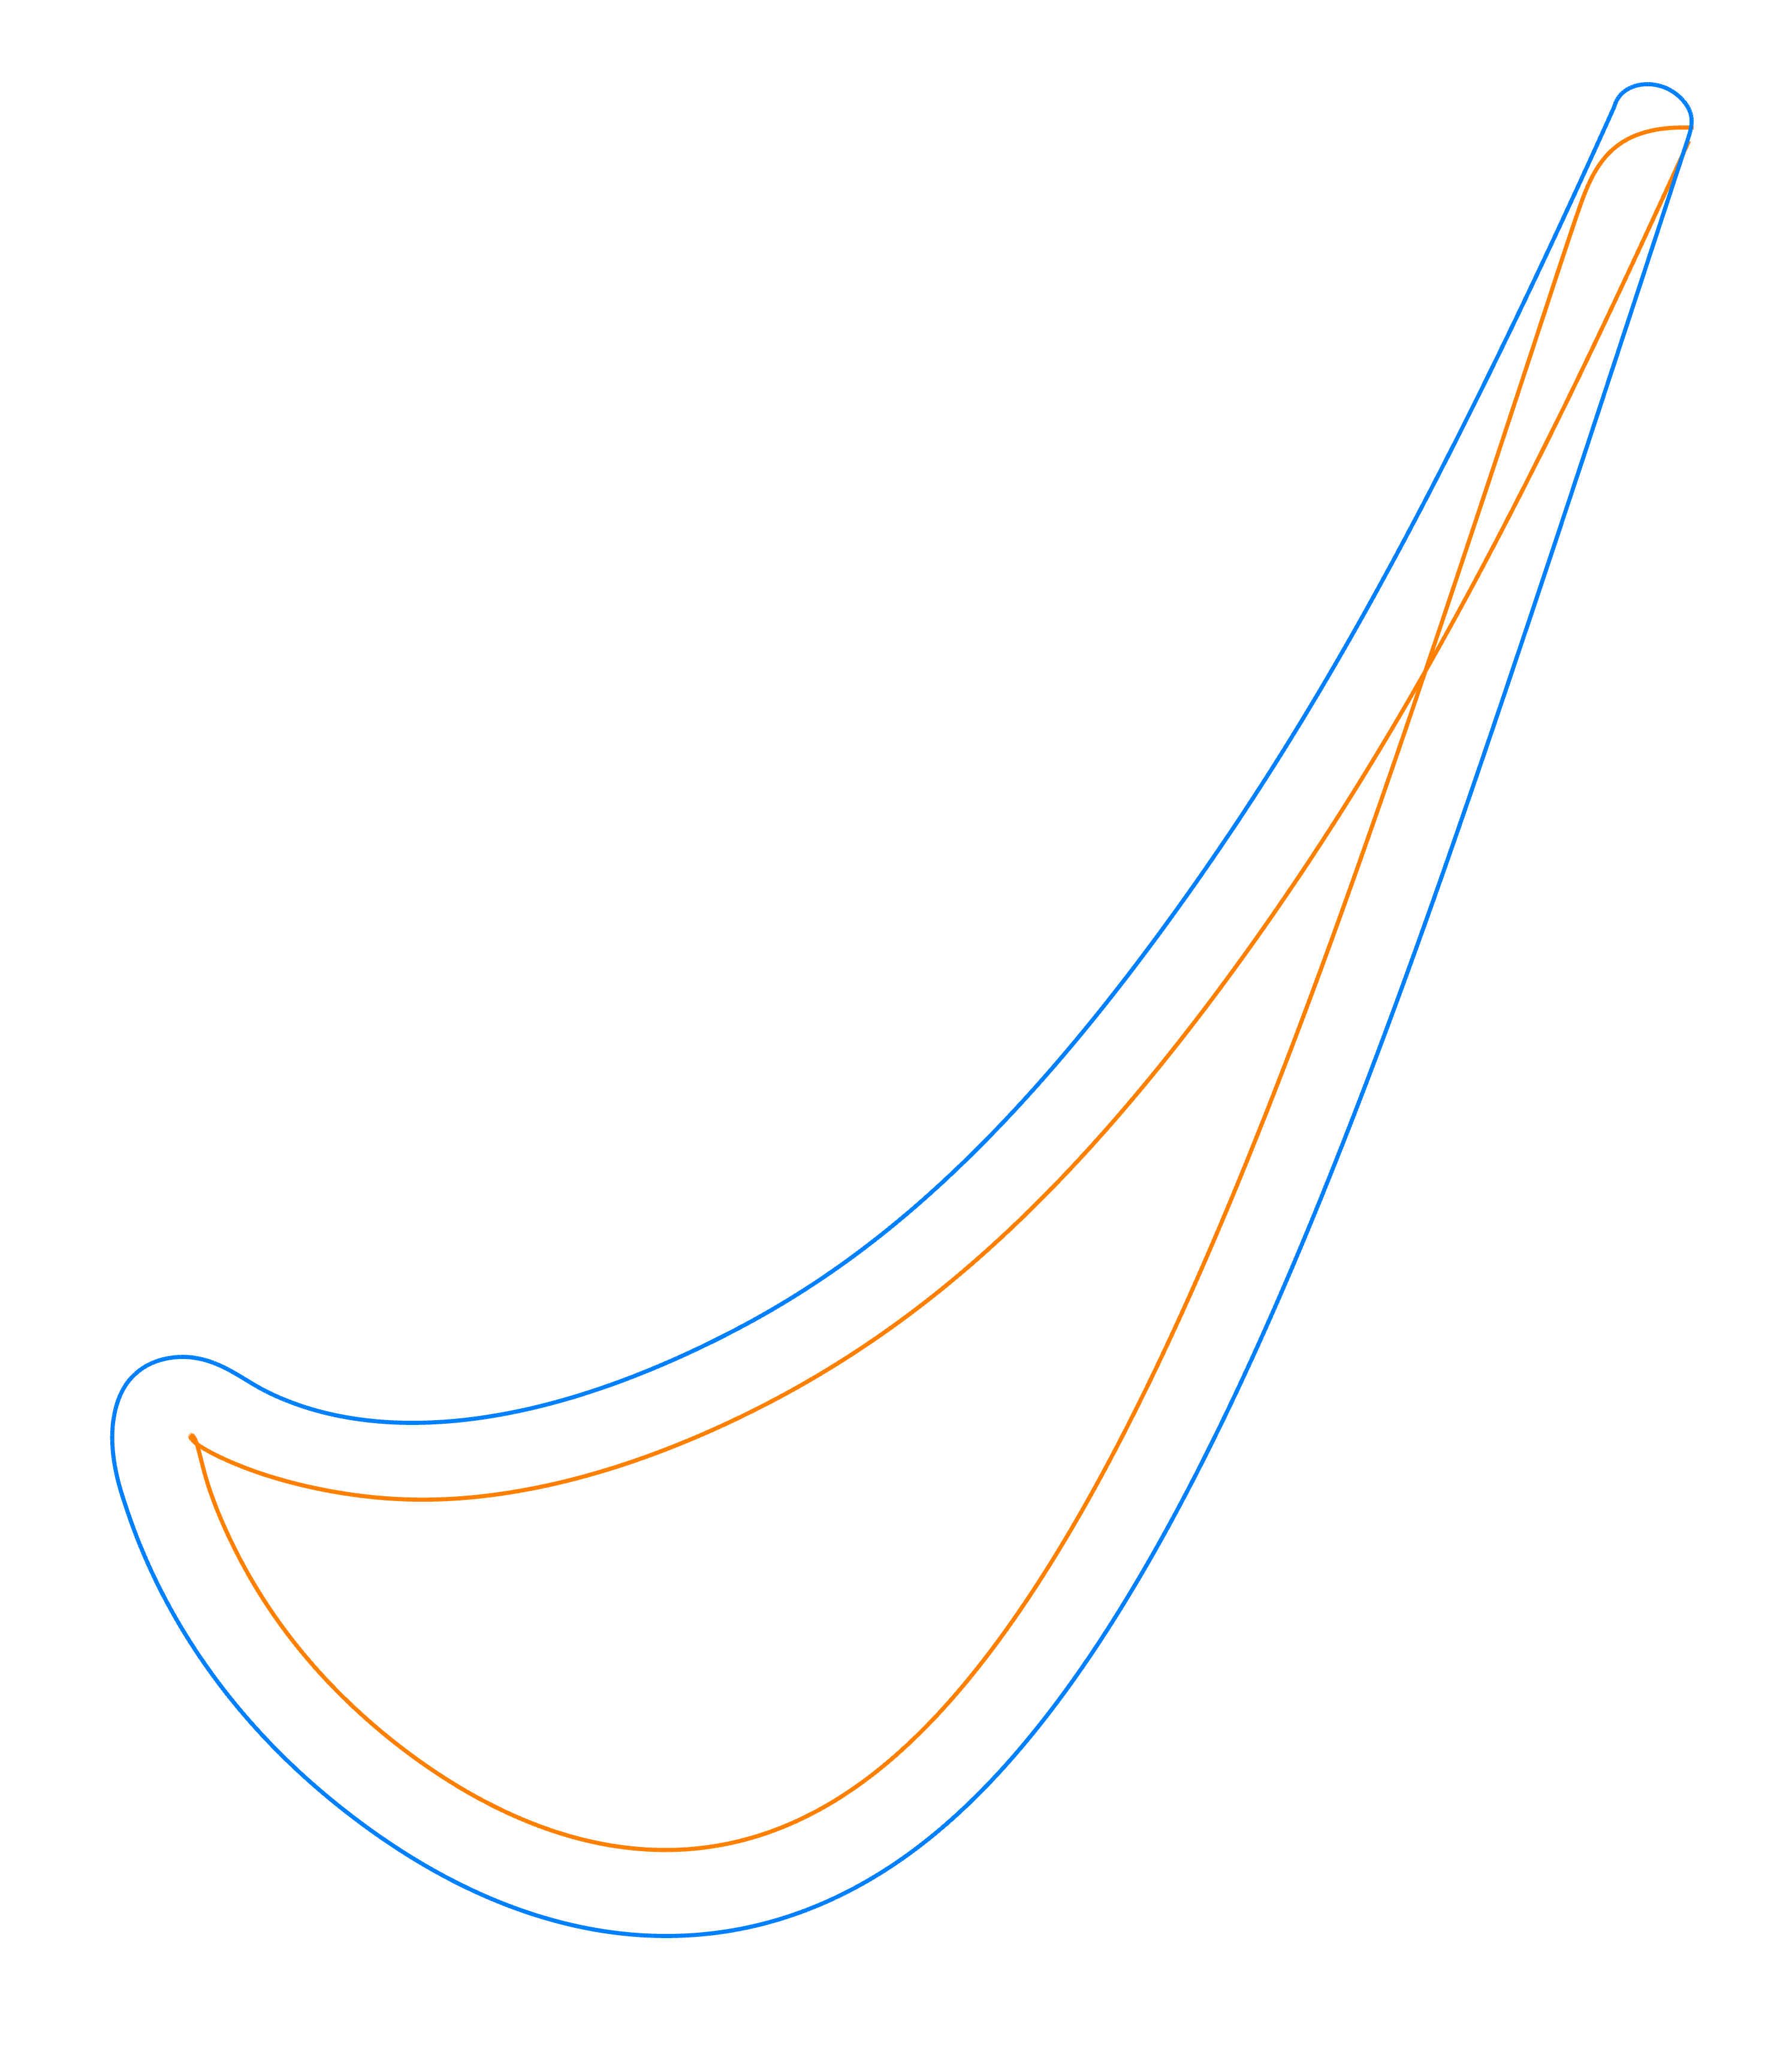
\includegraphics[width=\textwidth]{../../tec/shrinking/61.png}
				\caption{Profil und \textbf{Offset-Kurve}}
			\end{subfigure}
			\begin{subfigure}{.32\textwidth}
				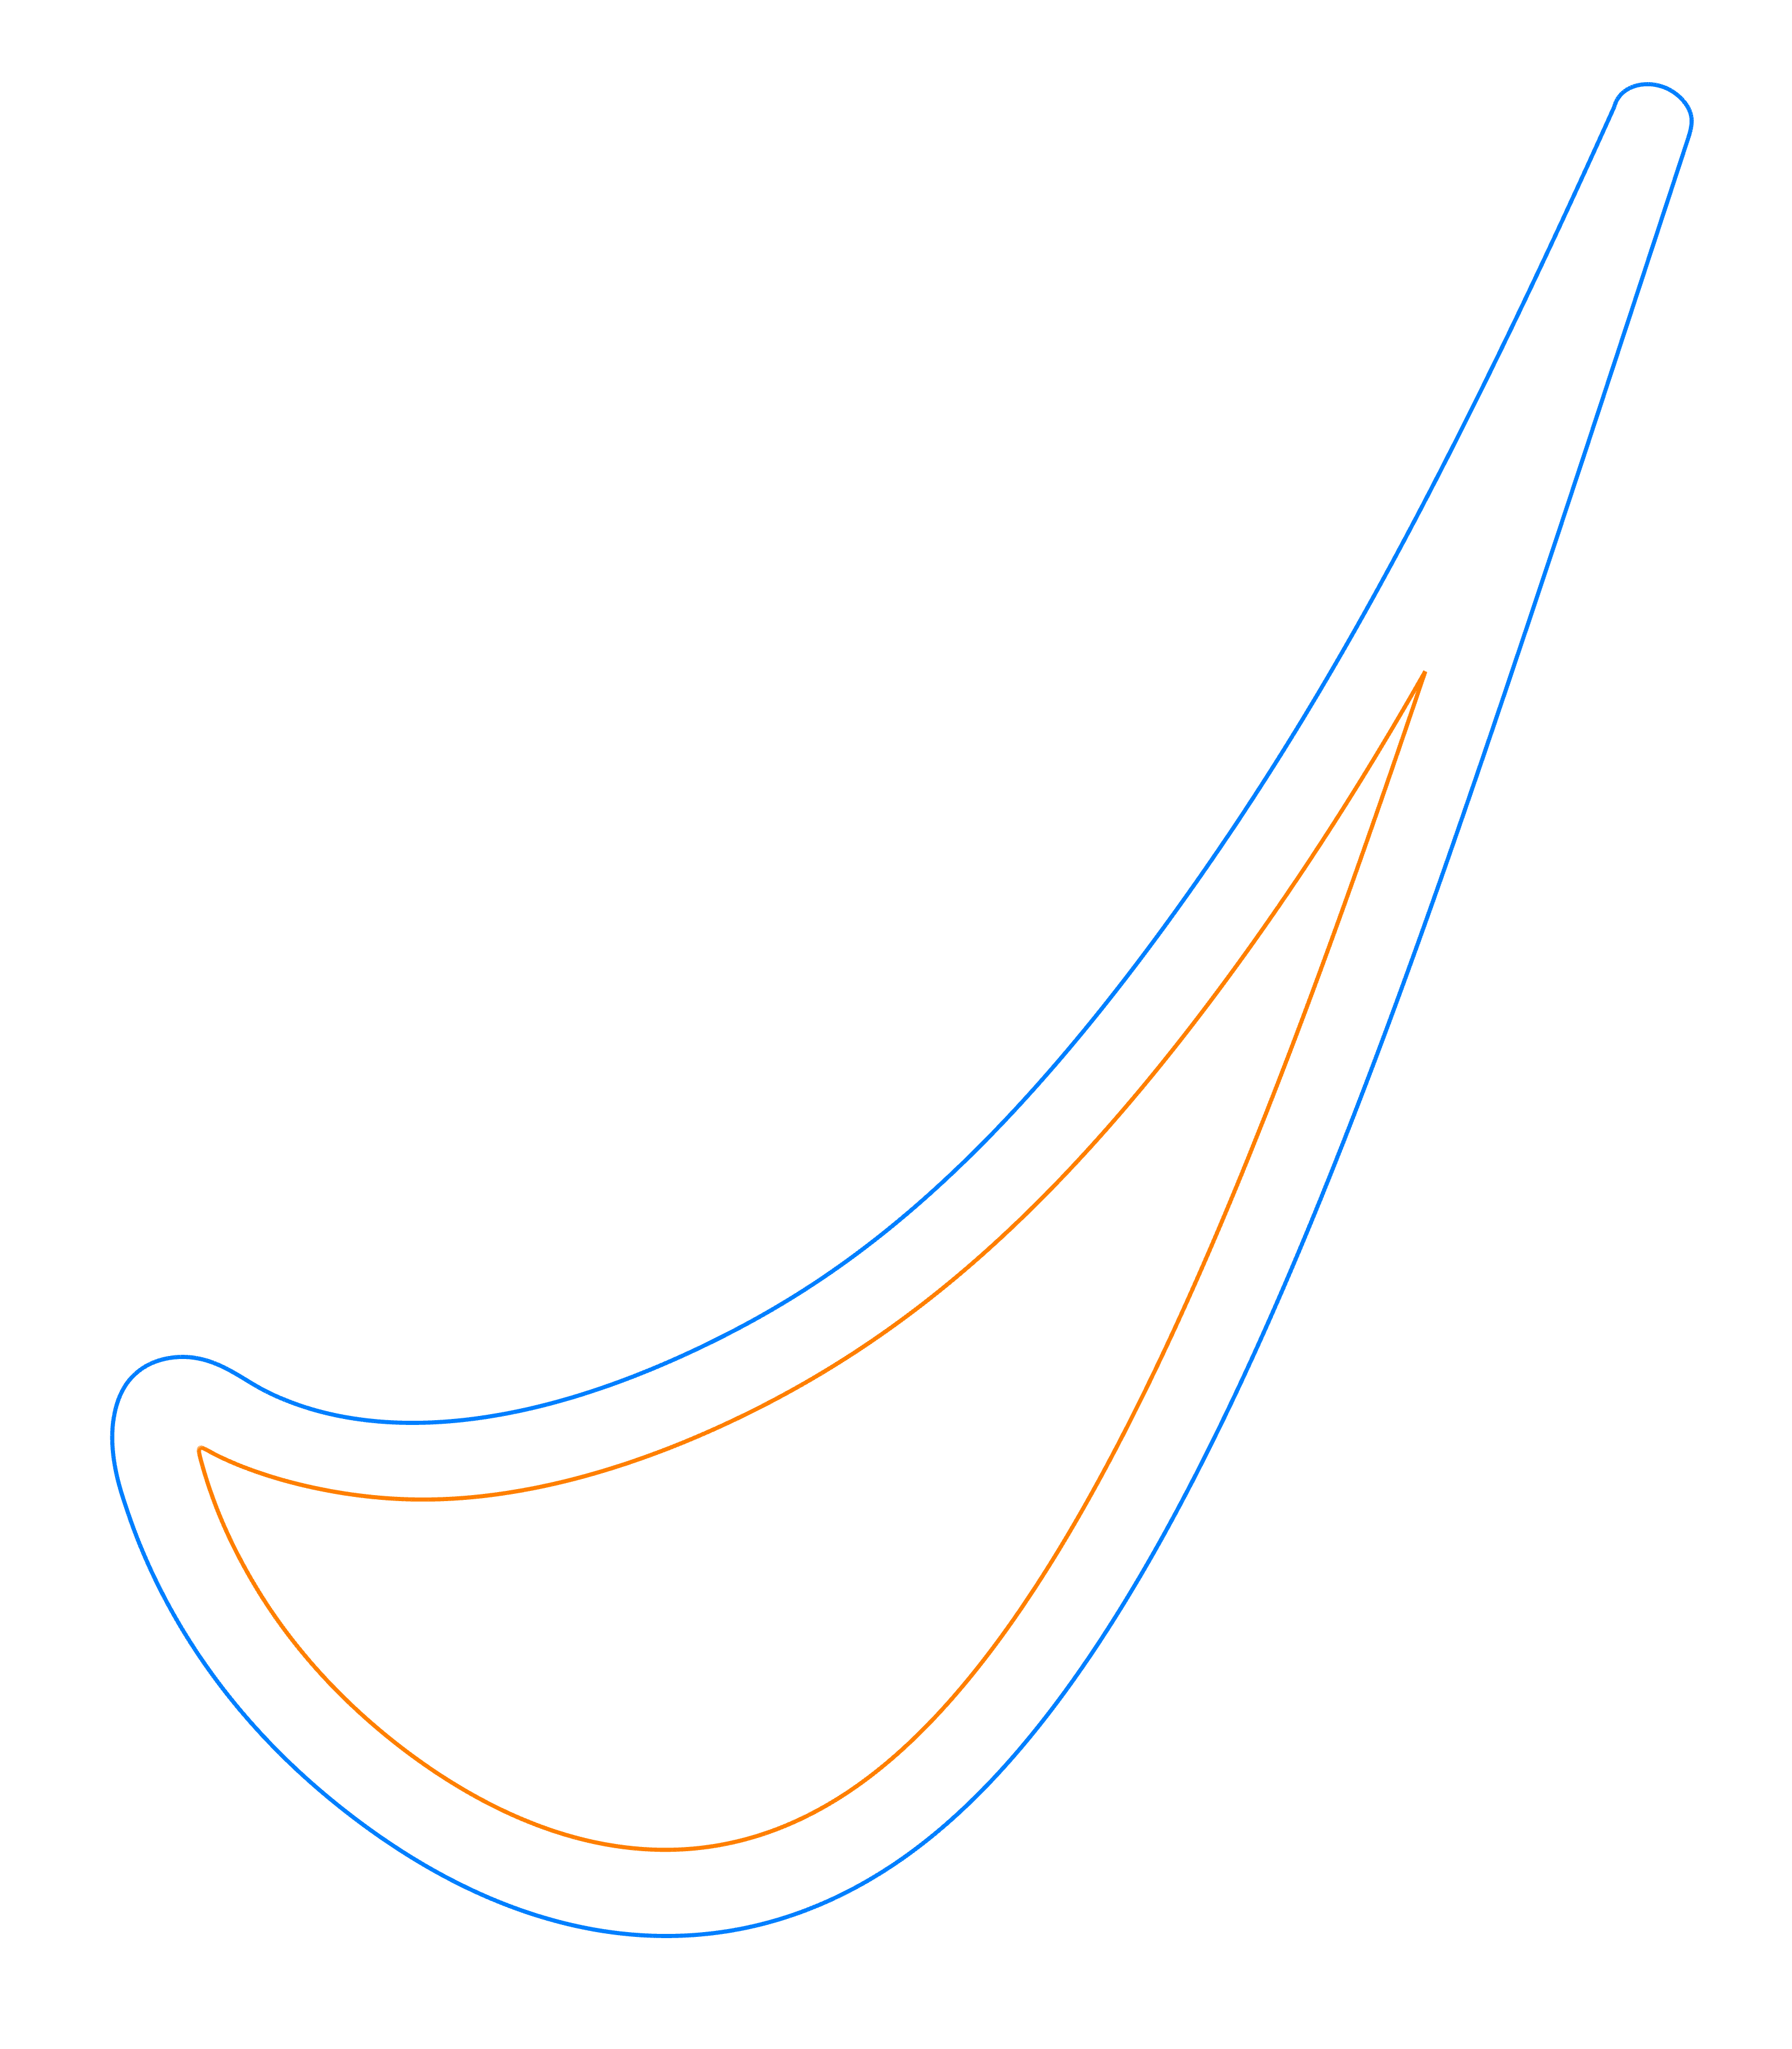
\includegraphics[width=\textwidth]{../../tec/shrinking/62.png}
				\caption{\textbf{Getrimmte} Offset-Kurve}
			\end{subfigure}
			\begin{subfigure}{.32\textwidth}
				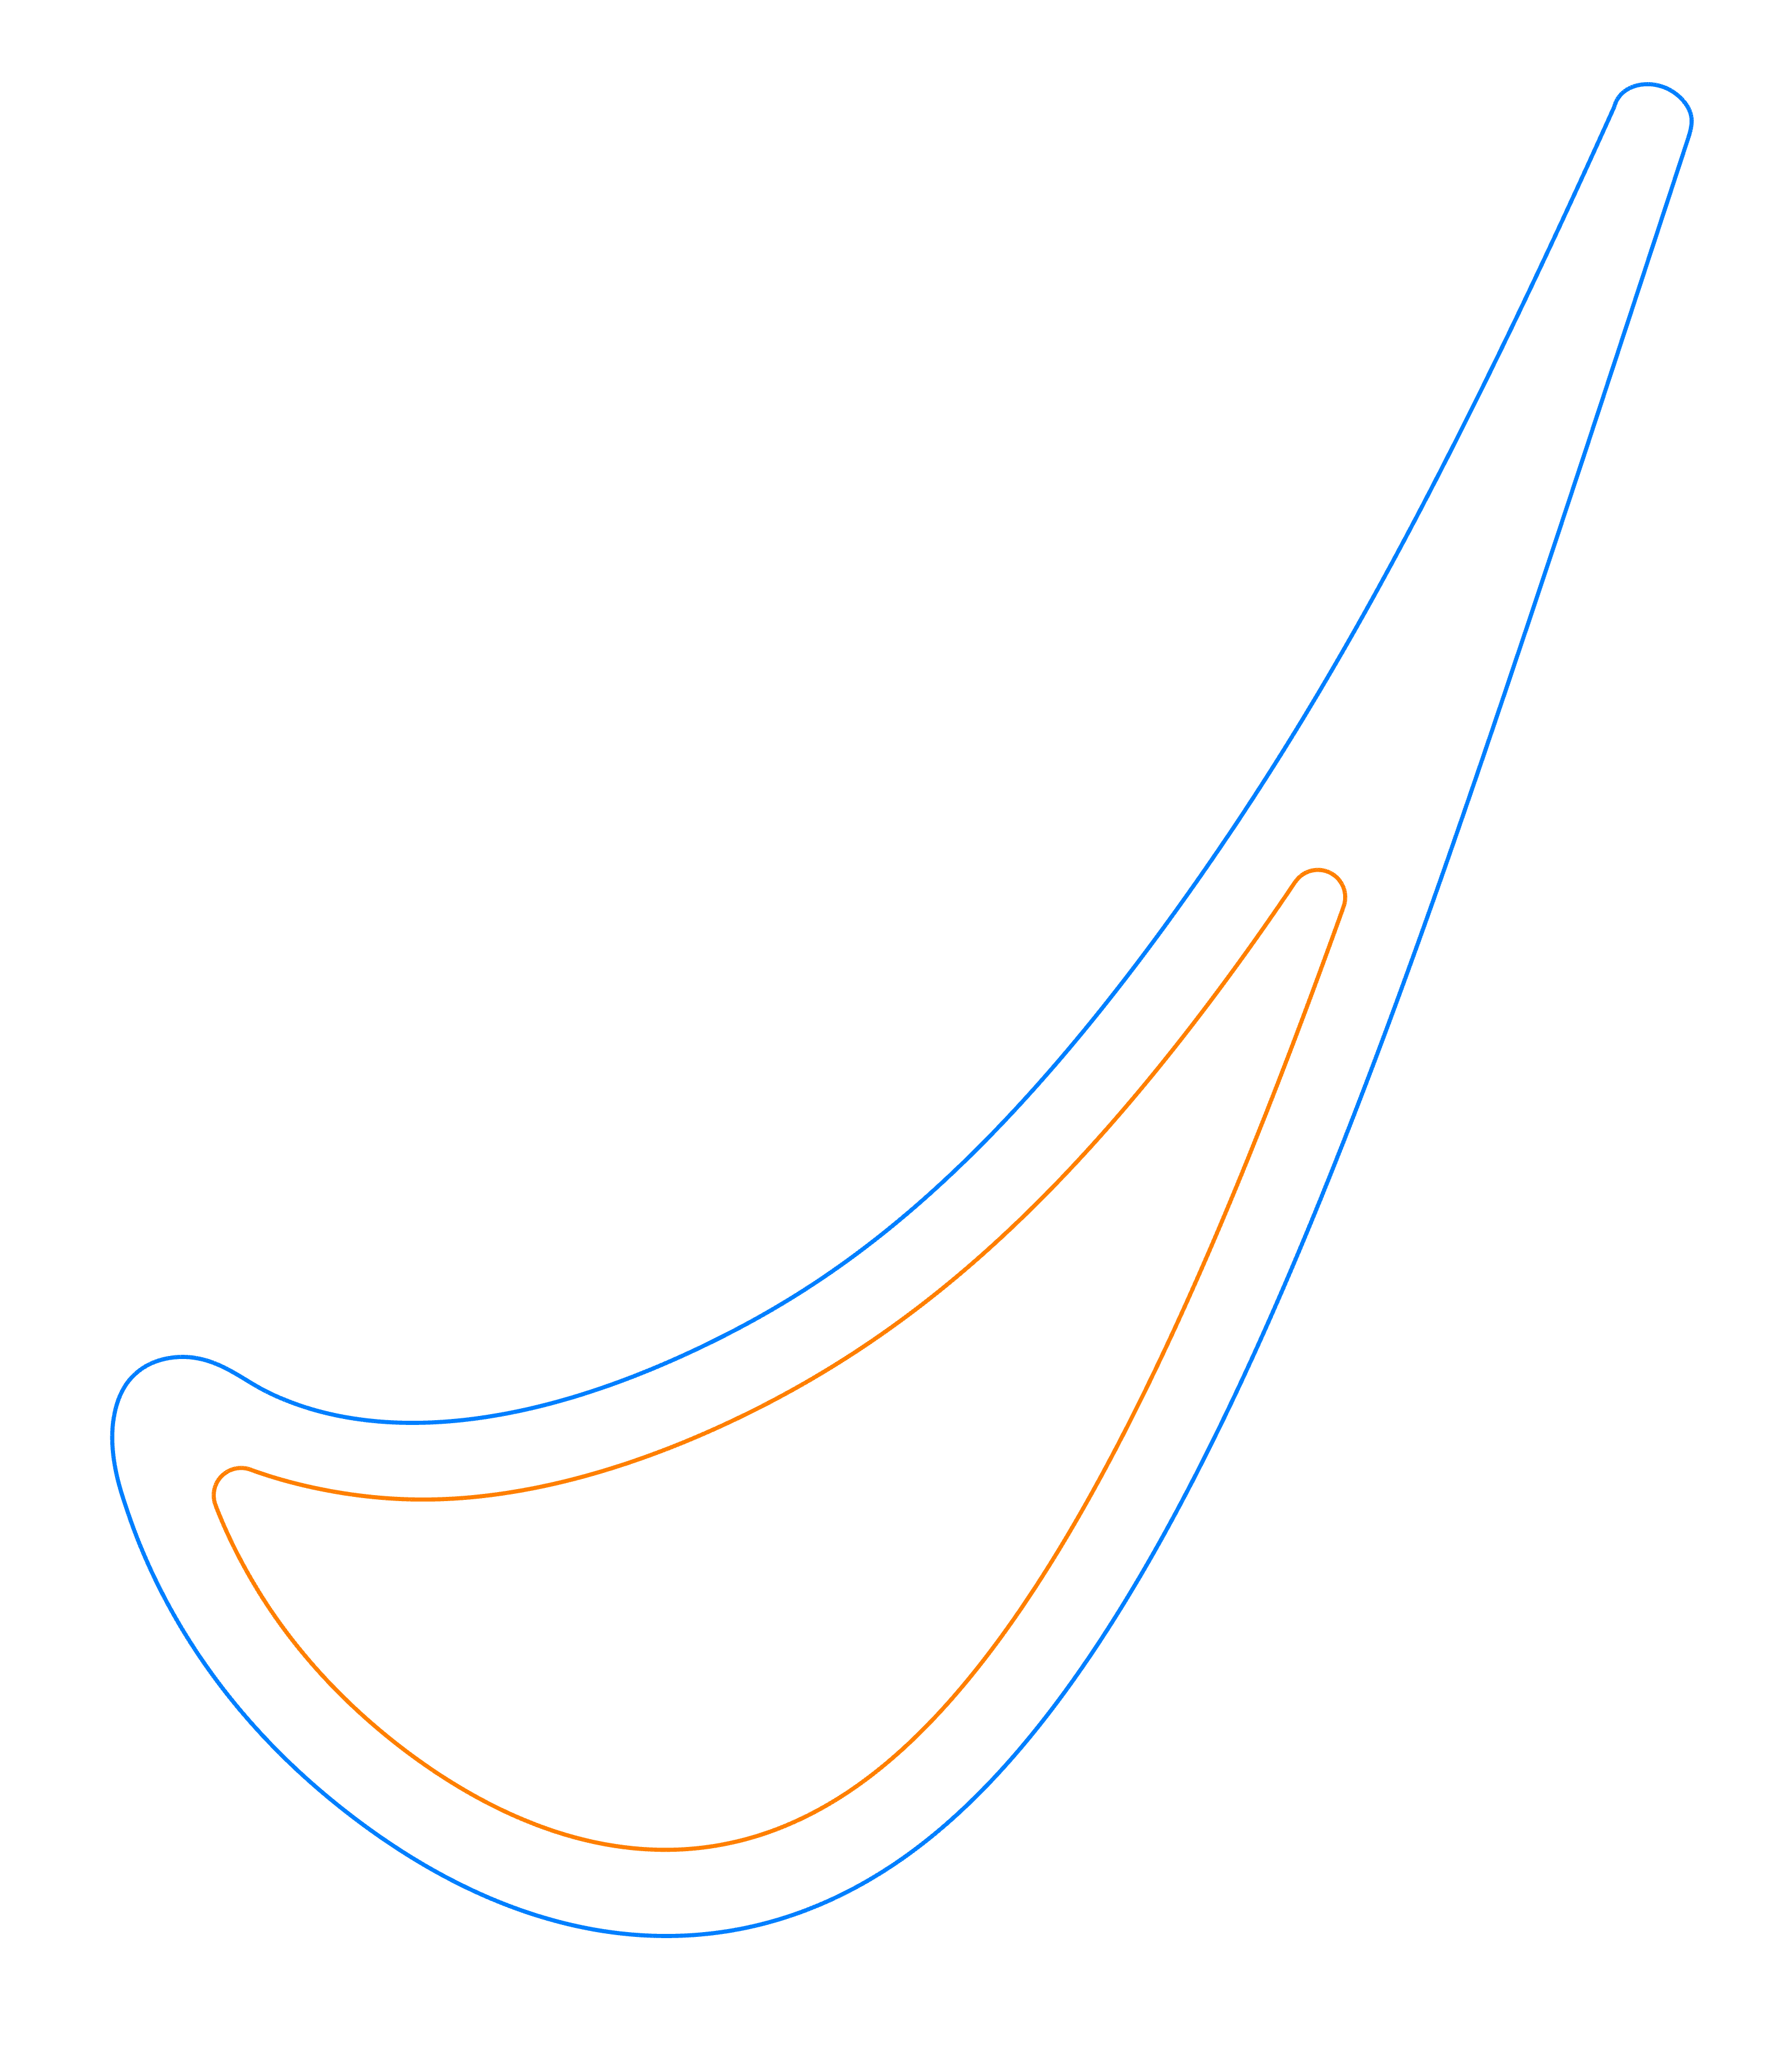
\includegraphics[width=\textwidth]{../../tec/shrinking/63.png}
				\caption{... mit \textbf{Fillets}!}
			\end{subfigure}
		\end{figure}
	\end{minipage}
	\vfill
\end{frame}

\begin{frame}
	\frametitle{Geometrien / Kanäle / Kammern}
	\vspace{-0.7cm}\hspace{-0.5cm}
	\centering
	\begin{minipage}[t]{\textwidth}
		\begin{figure}[H]
			\centering
			\begin{subfigure}[t]{.5\textwidth}
				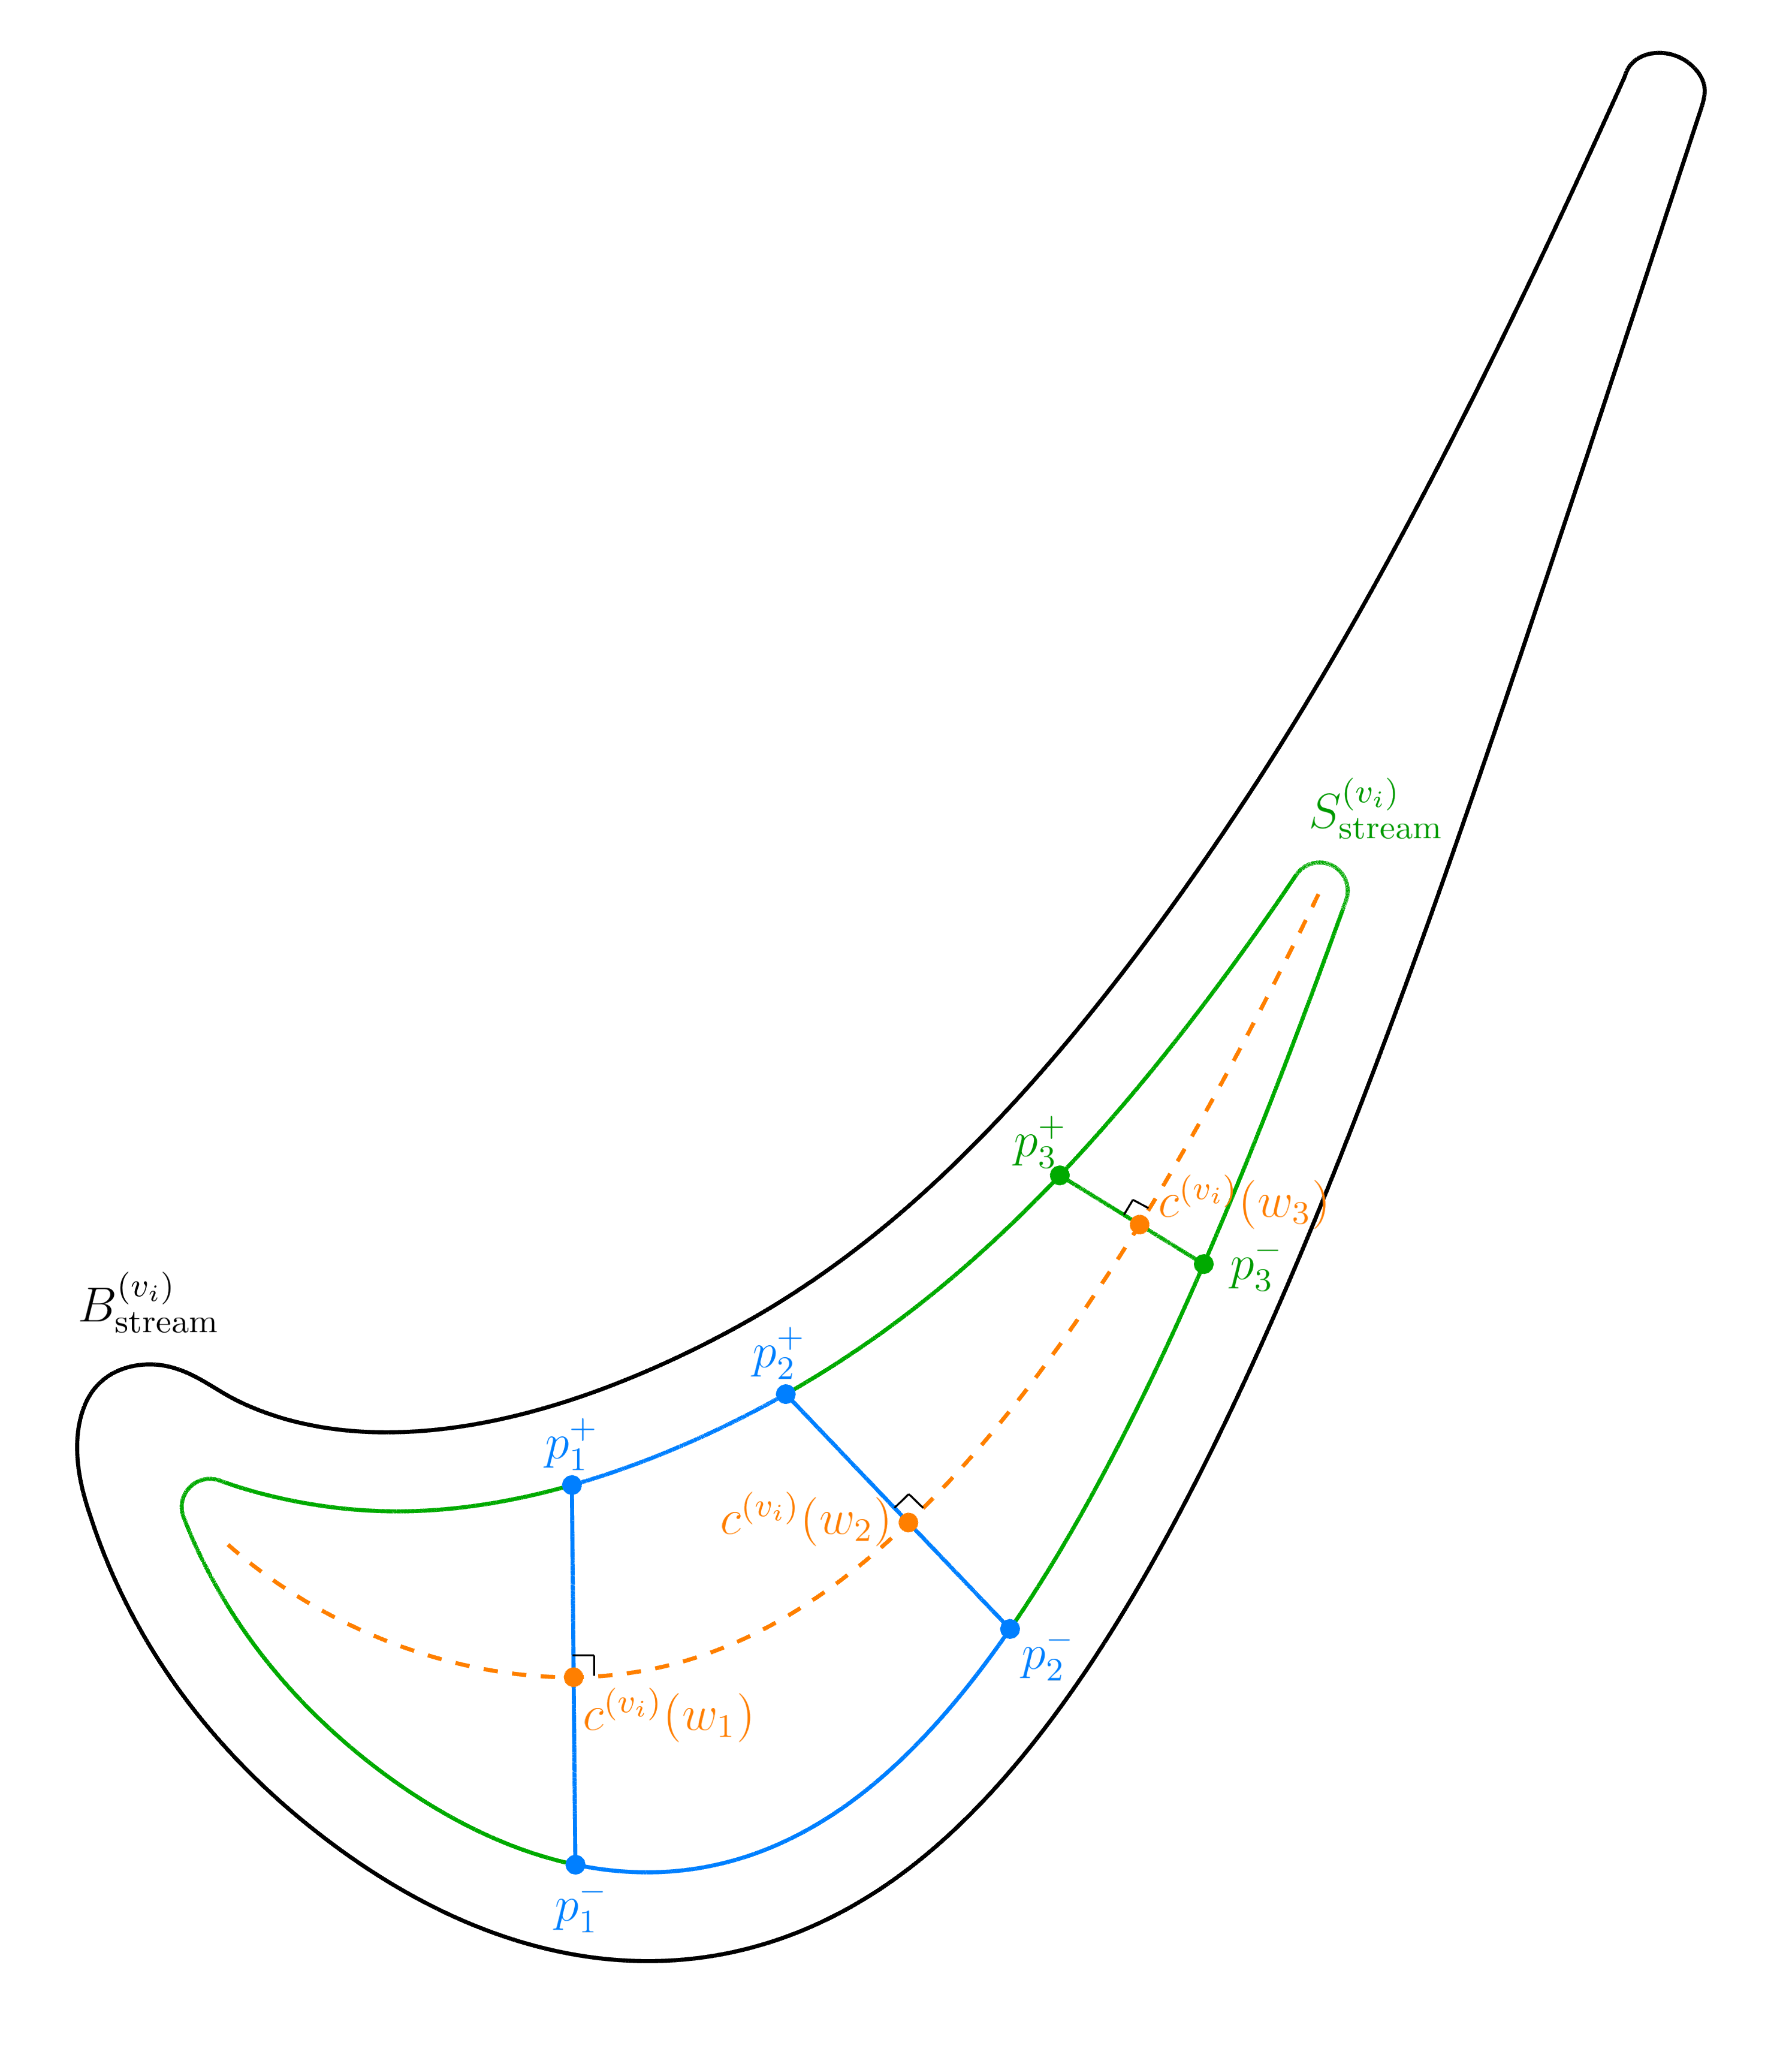
\includegraphics[width=.8\textwidth]{../../tec/chambers/61.png}
				\caption{Partitionierung des Profils.}
			\end{subfigure}
			\begin{subfigure}{.39\textwidth}
				Entlang der \textbf{Skelettlinie} kann man nun Wand-positionen und -winkel festlegen, um mehrere Kammern zu erhalten.\\

				\centering
				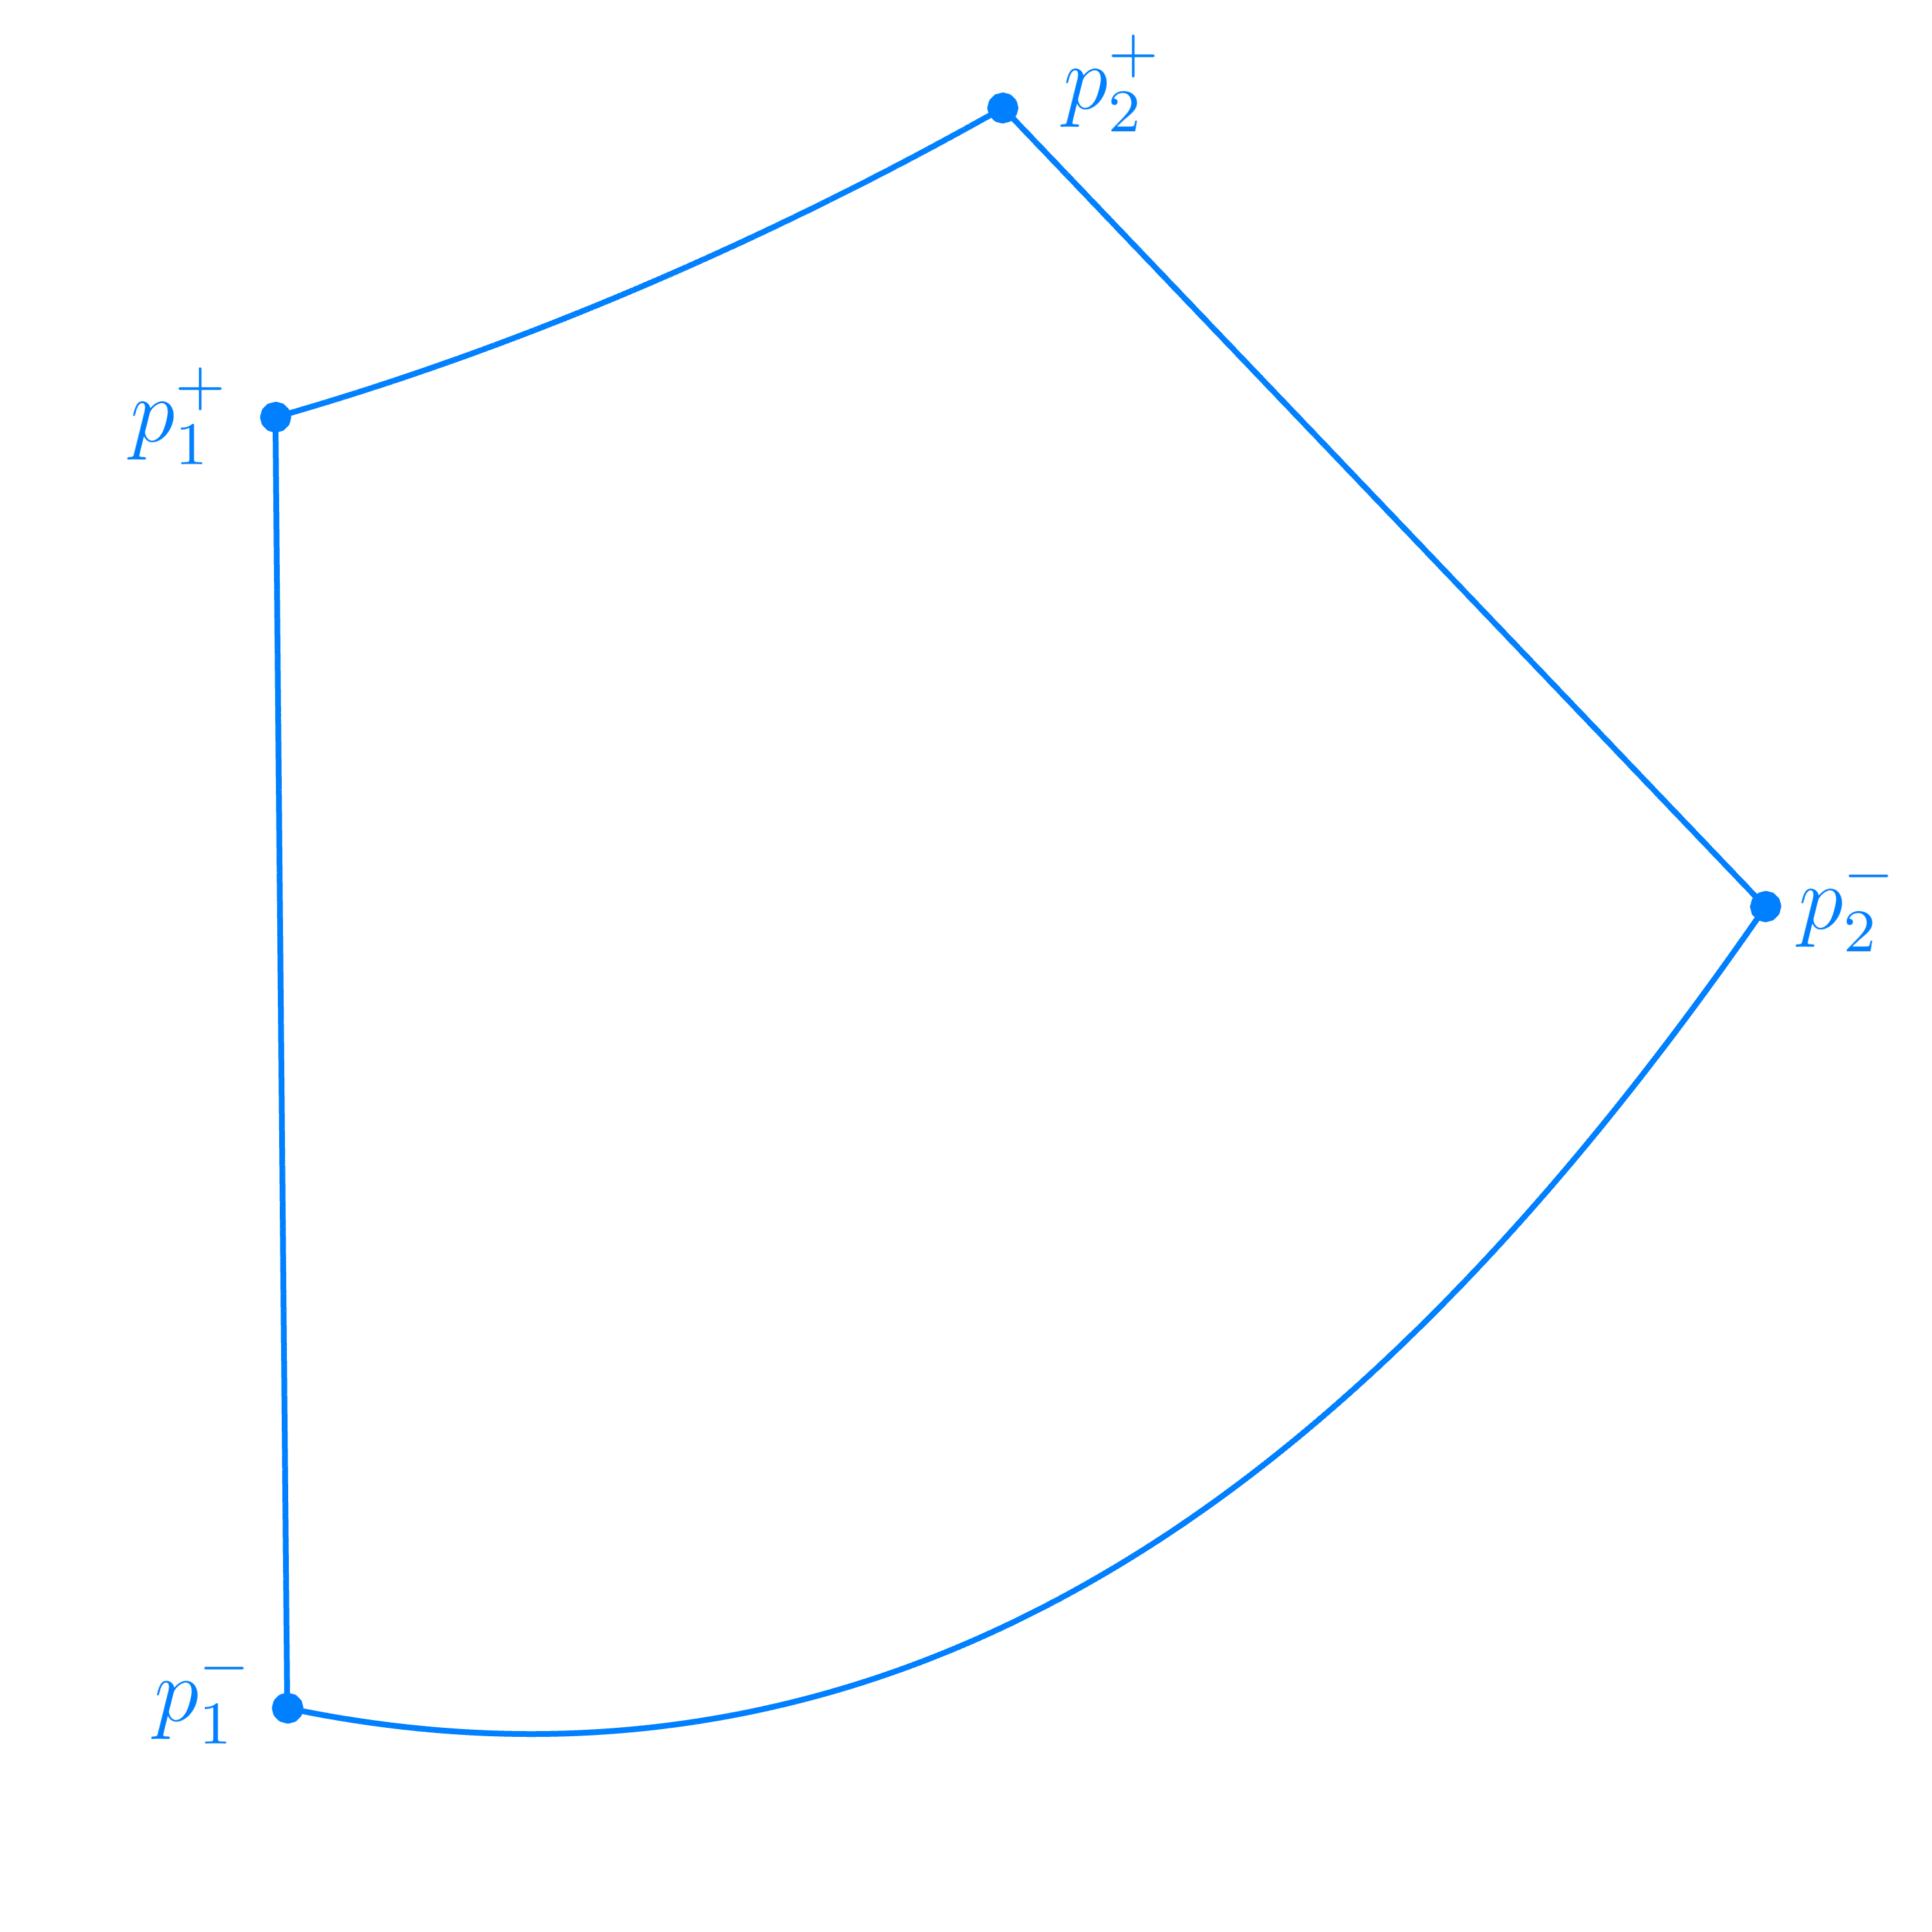
\includegraphics[width=.85\textwidth]{../../tec/chambers/62.png}
				\caption{Eine resultierende Partition.}
			\end{subfigure}
		\end{figure}
	\end{minipage}
	\vfill
\end{frame}

\begin{frame}
	\frametitle{Geometrien / Kanäle / Kammern}
	\vspace{-0.25cm}\hspace{-0.5cm}
	\centering
	\begin{minipage}[t]{\textwidth}
		Wie vorhin:
		\begin{figure}[H]
			\begin{subfigure}{.32\textwidth}
				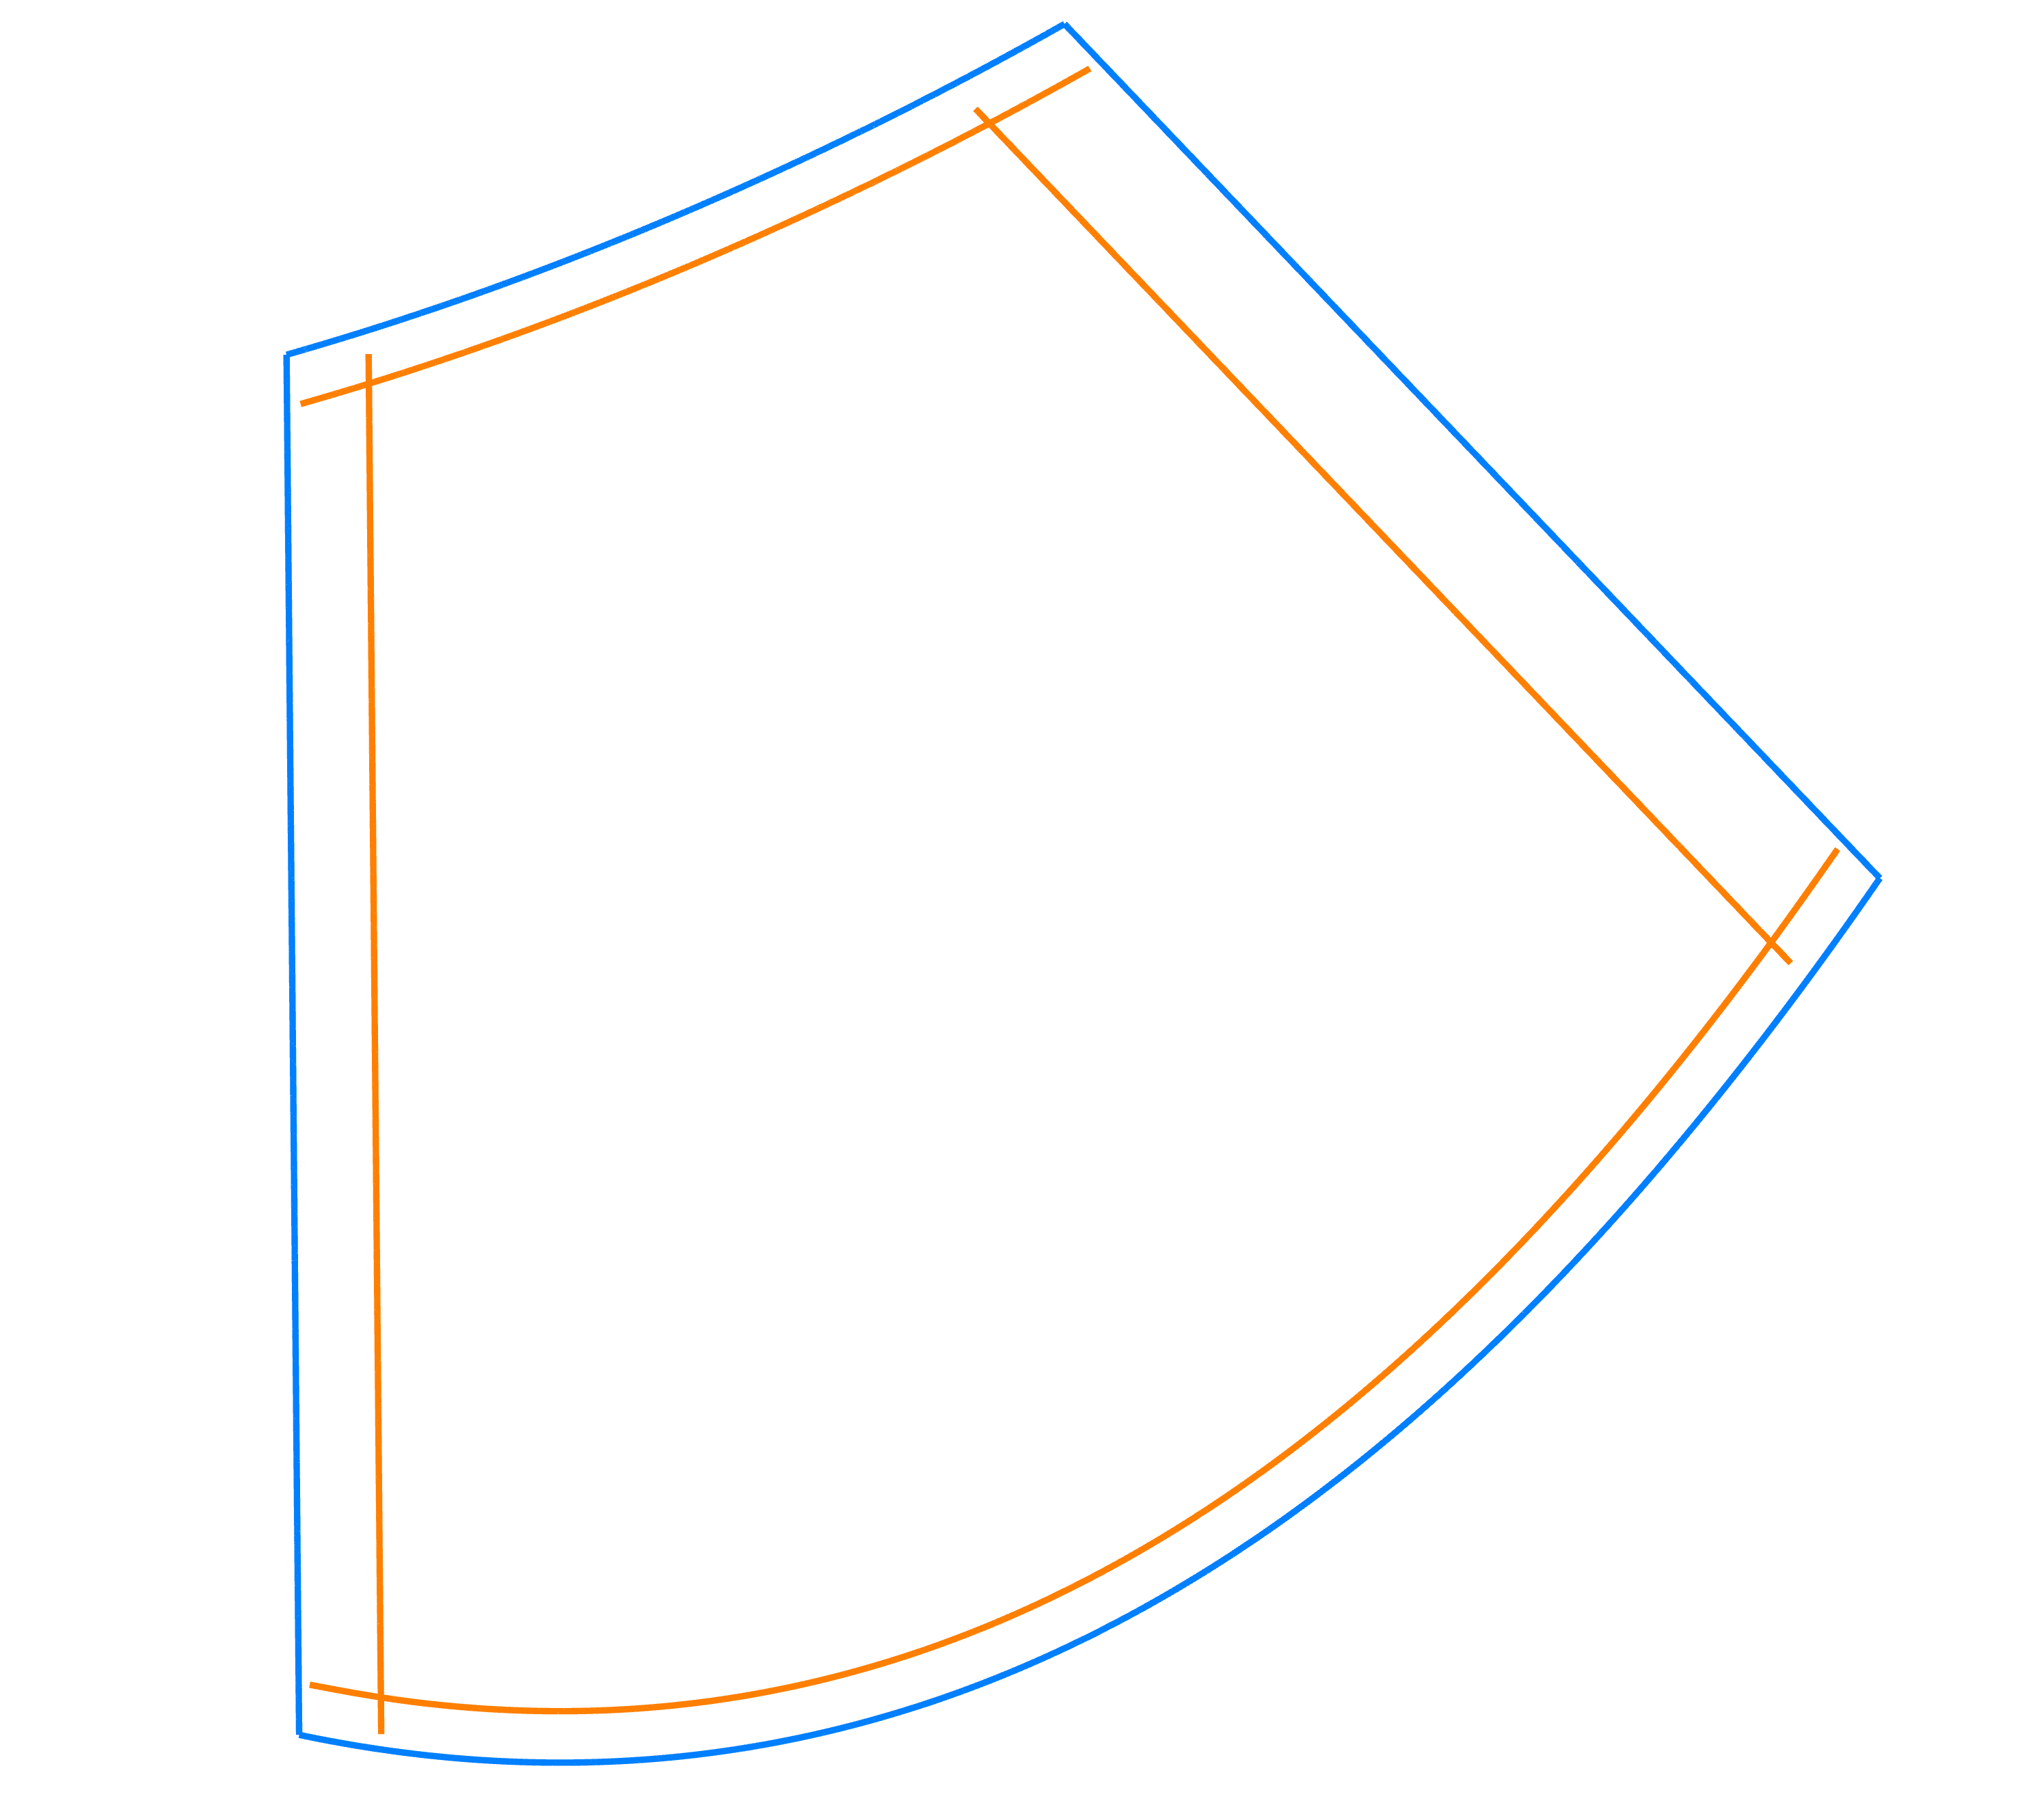
\includegraphics[width=\textwidth]{../../tec/chambers/81.png}
				\caption{\textbf{Offset-Kurven} bilden,}
			\end{subfigure}
			\begin{subfigure}{.32\textwidth}
				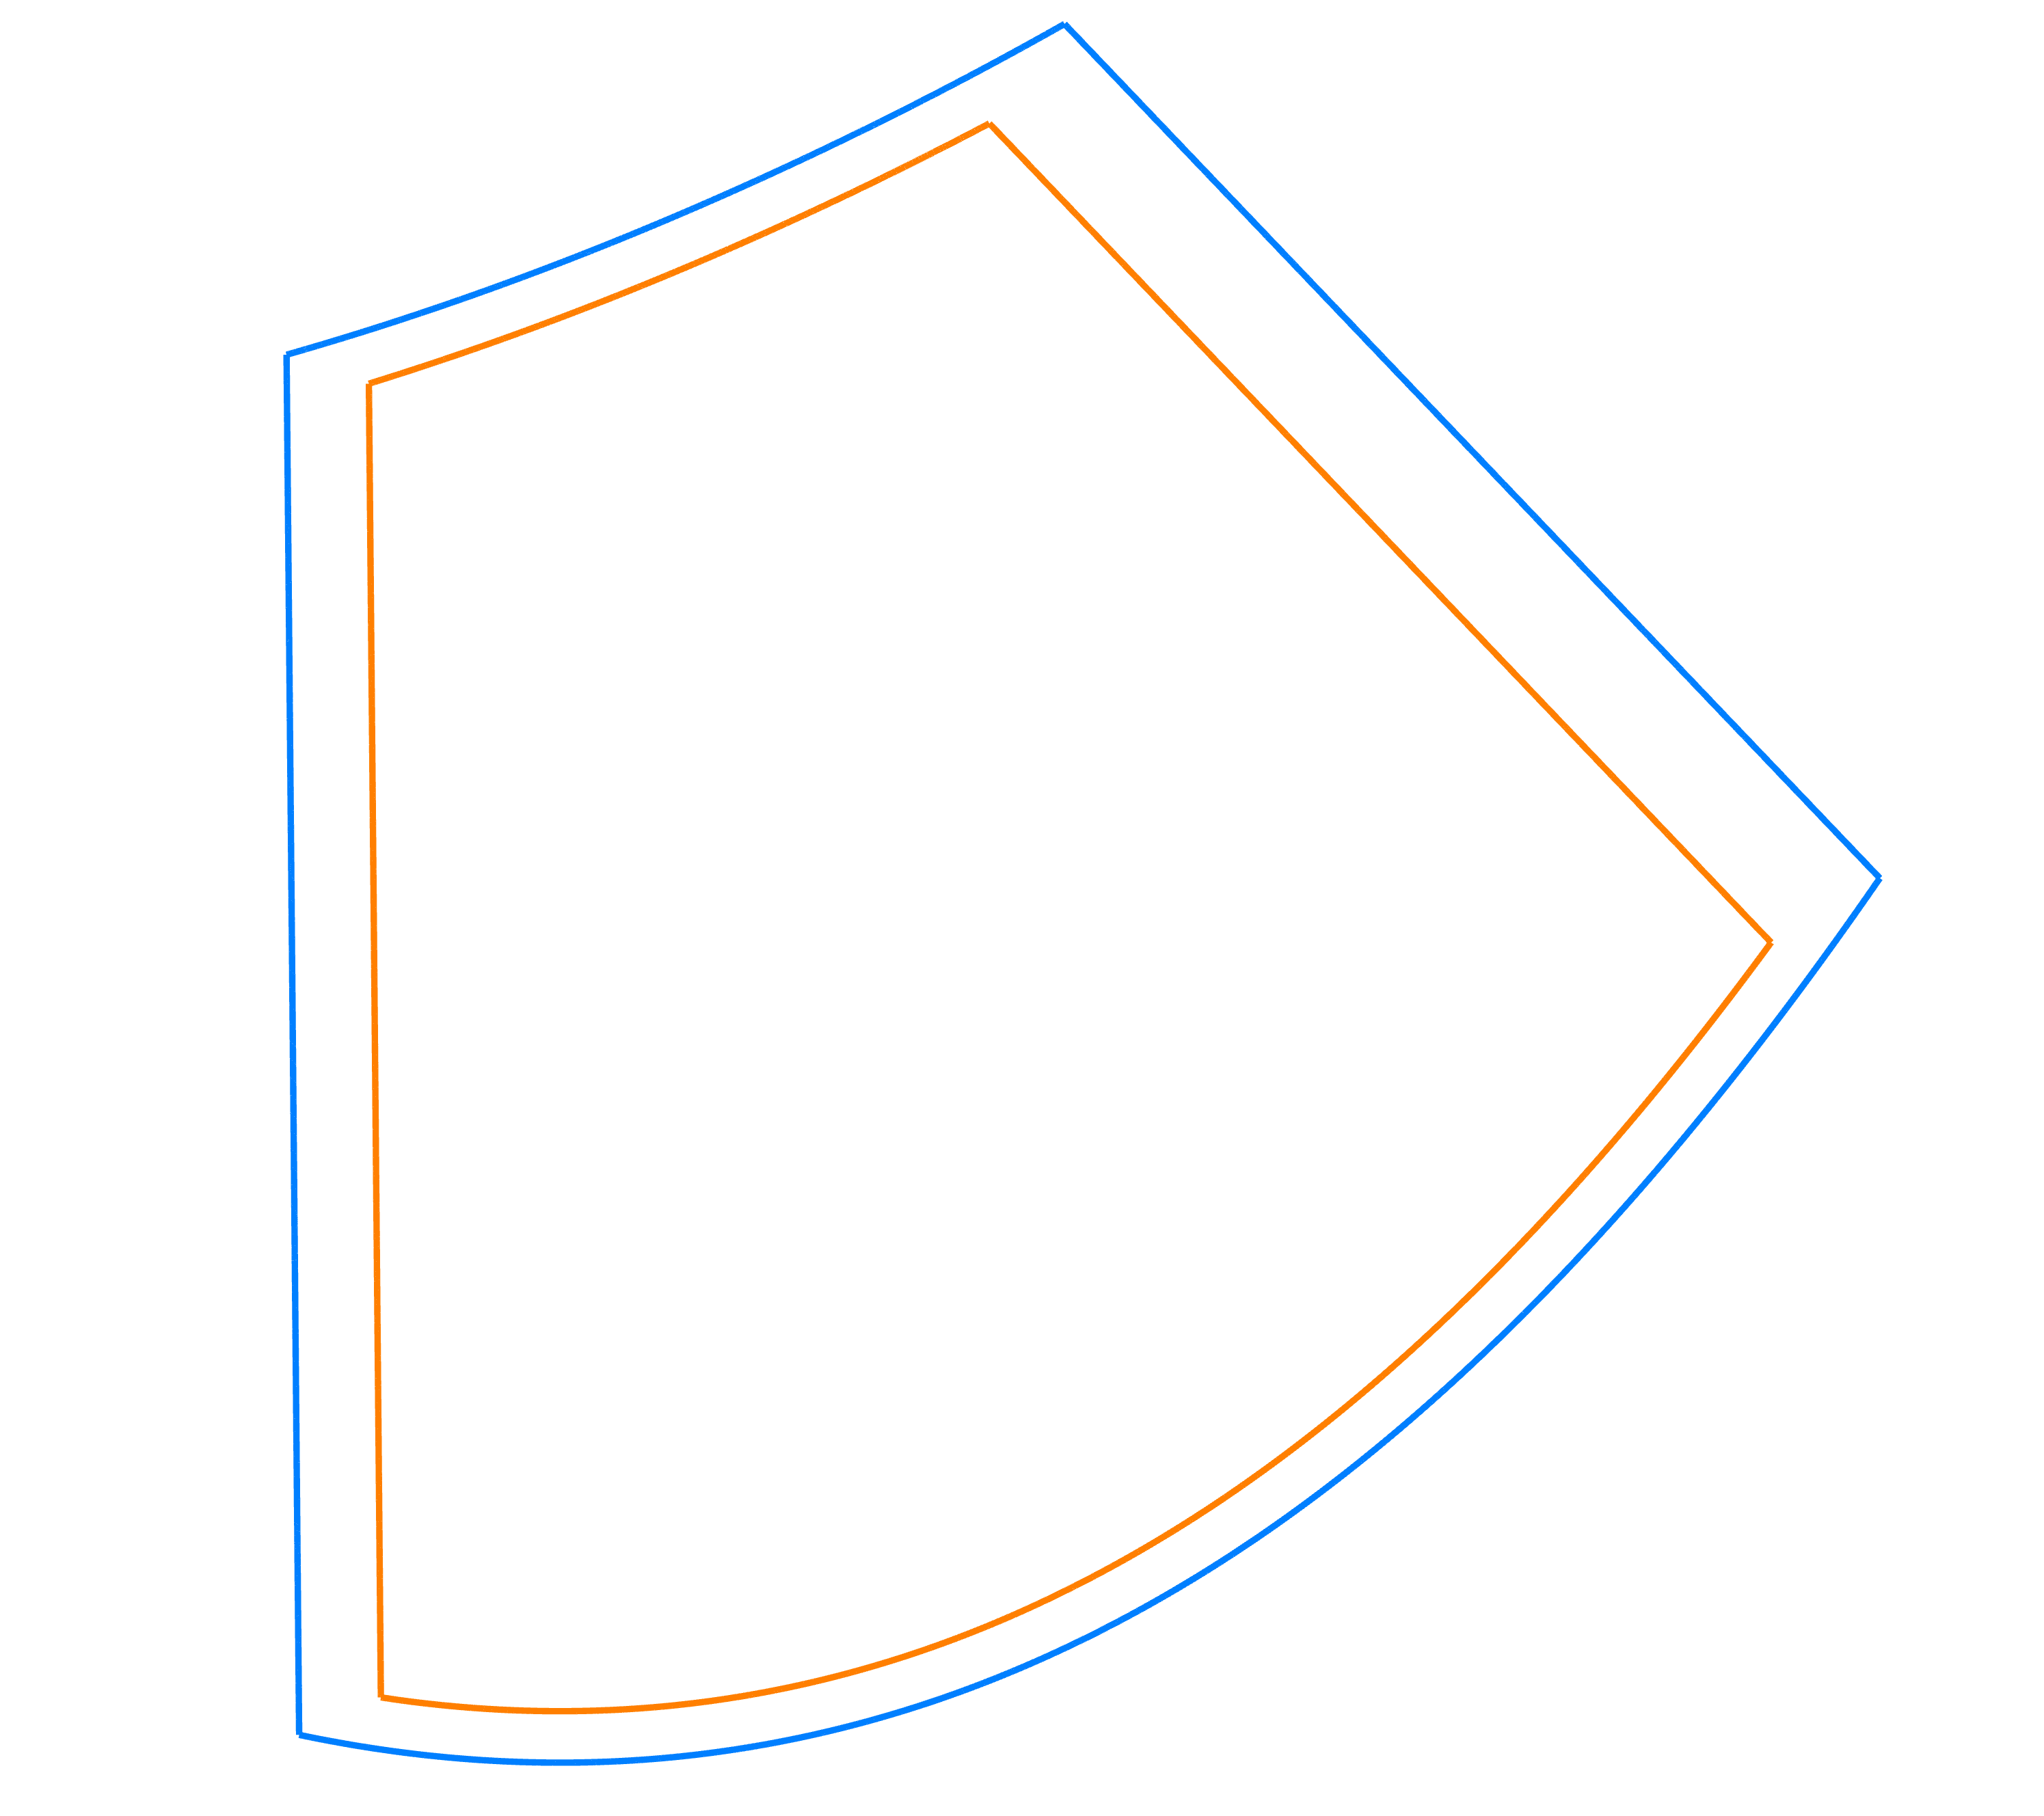
\includegraphics[width=\textwidth]{../../tec/chambers/82.png}
				\caption{an Schnittpunkten \textbf{trimmen},}
			\end{subfigure}
			\begin{subfigure}{.32\textwidth}
				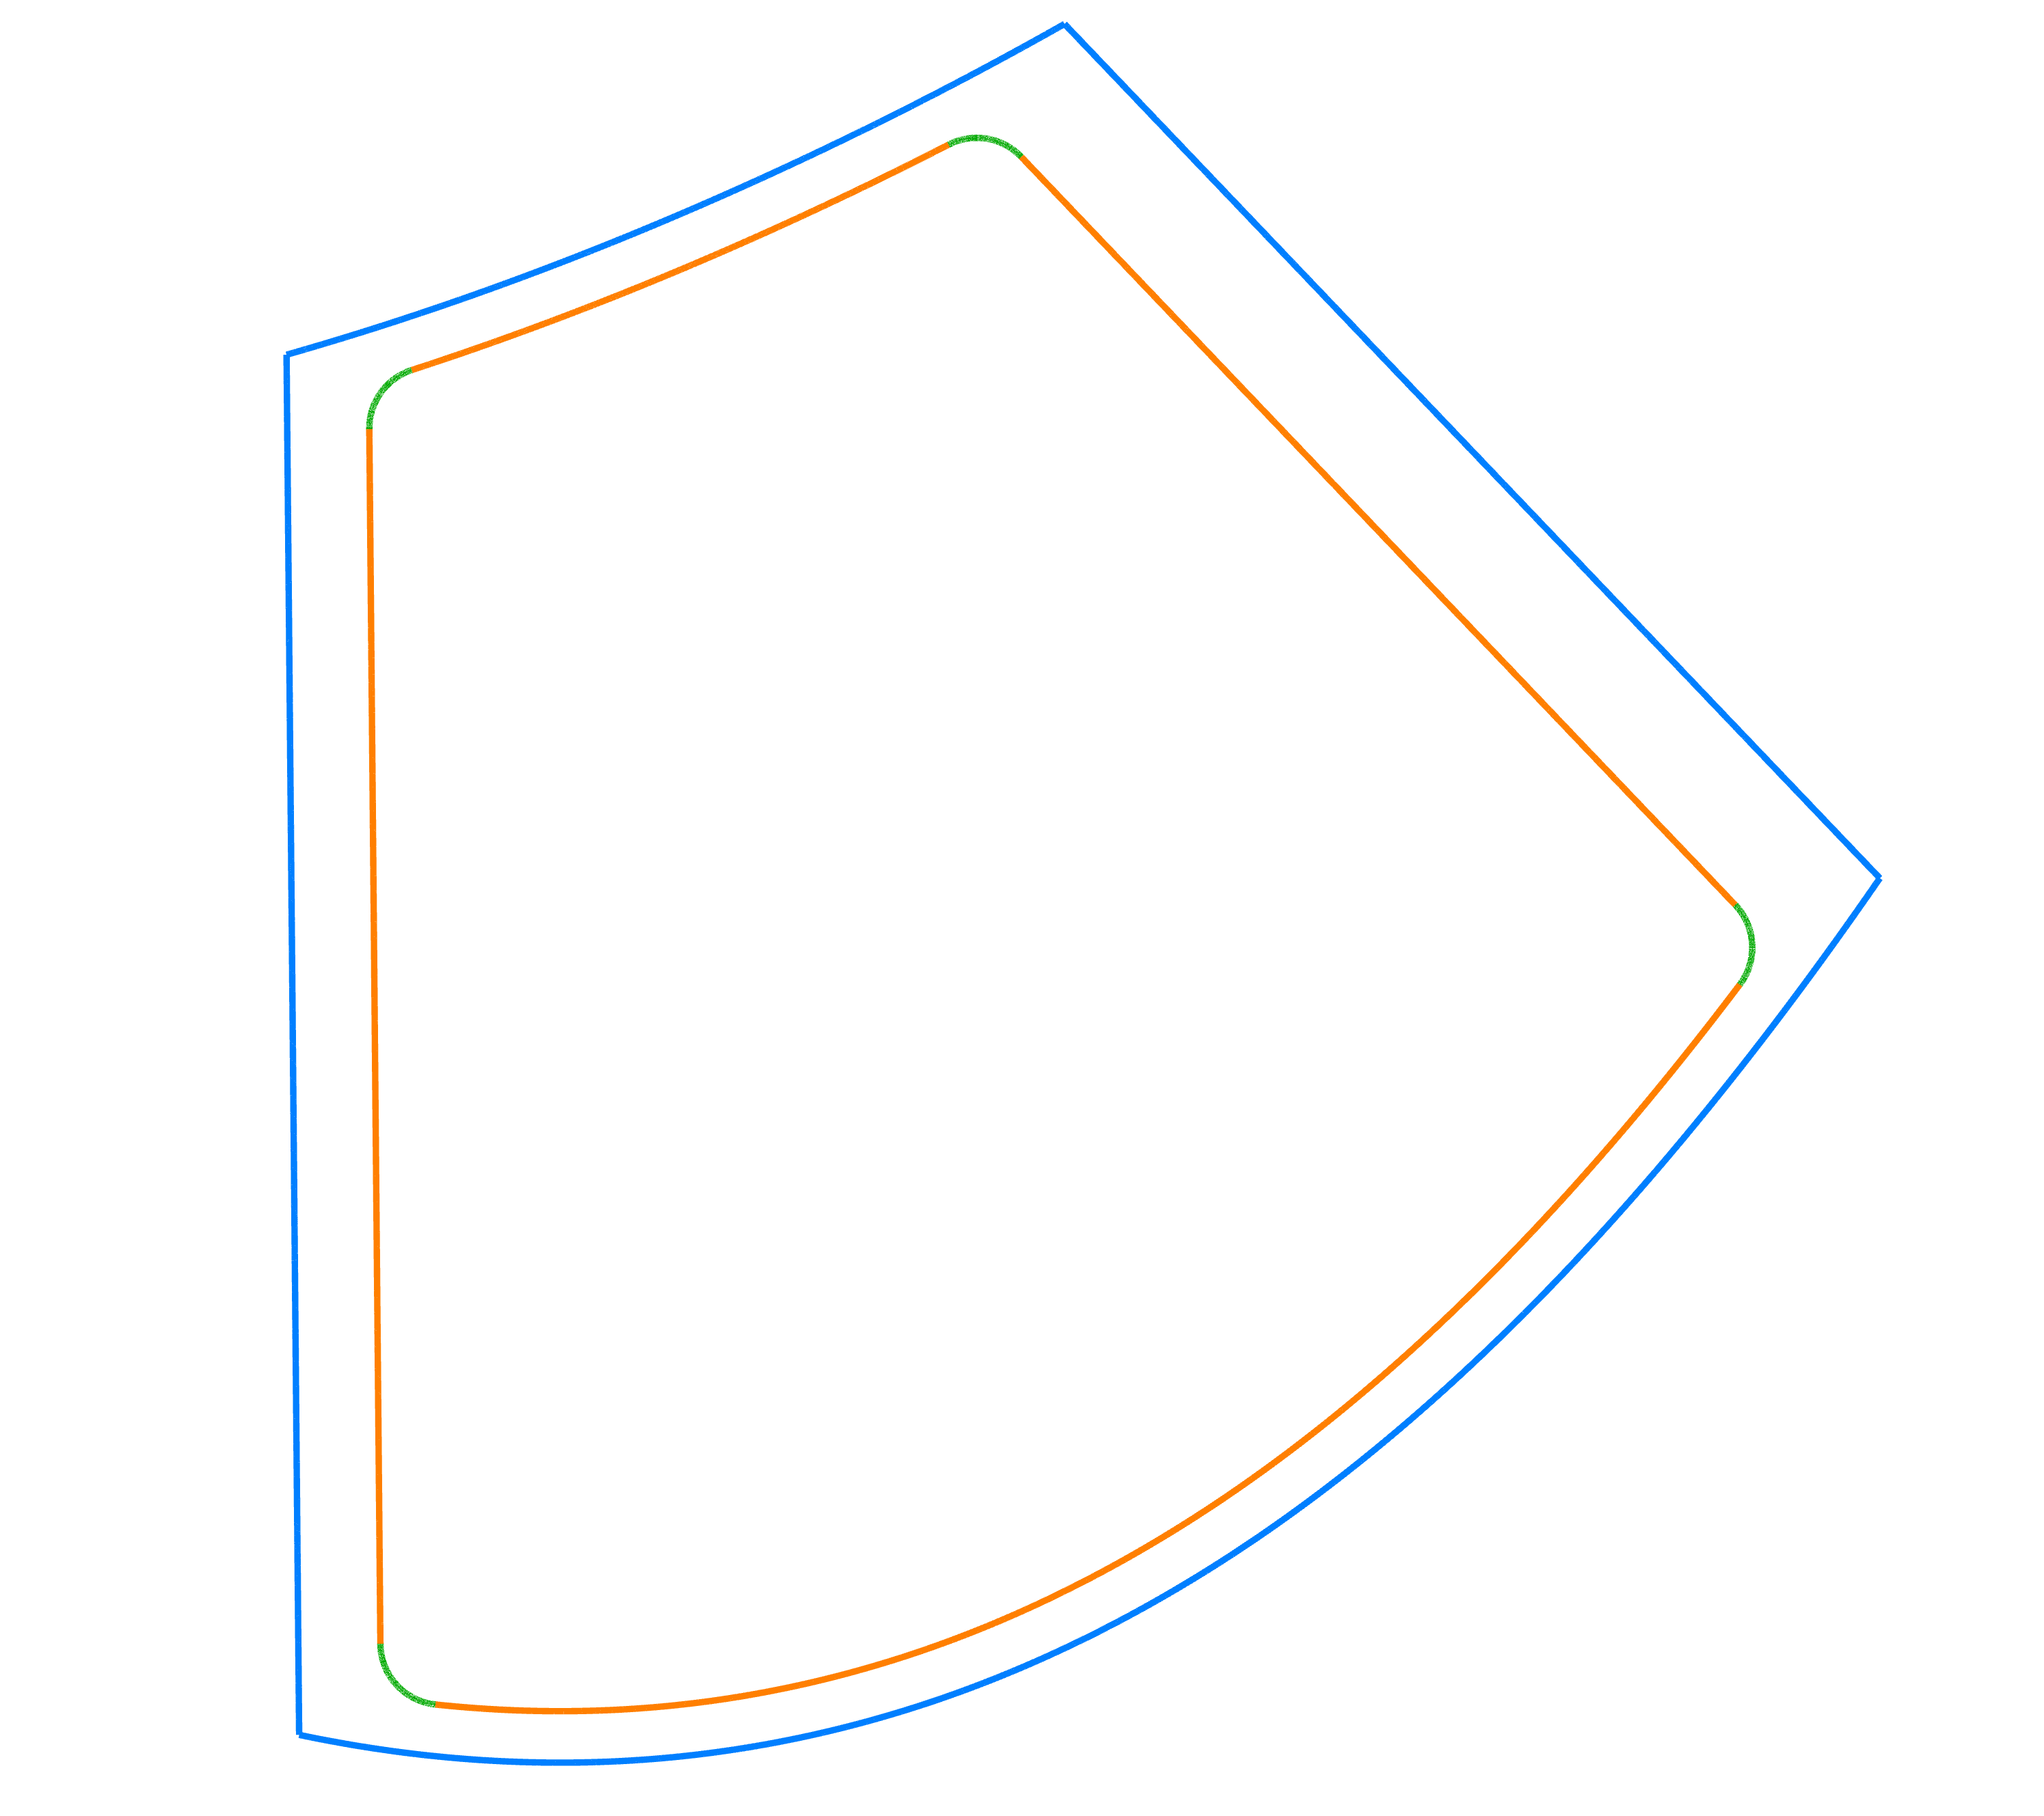
\includegraphics[width=\textwidth]{../../tec/chambers/83.png}
				\caption{und \textbf{Fillets} hinzufügen.}
			\end{subfigure}
			\label{fig:chamber_shrinking}
		\end{figure}
		So erhalten wir ein \textbf{Kammerprofil}.
	\end{minipage}
	\vfill
\end{frame}

\begin{frame}
	\frametitle{Geometrien / Kanäle / Kammern / Fillets}
	\vspace{-0.25cm}\hspace{-0.5cm}
	\centering
	\begin{minipage}[t]{\textwidth}
		Wie kriegt man \textbf{Fillets} mit Radius $r$? Wir finden den Schnittpunkt der \textbf{$r$-Offset-Kurven}:
		\begin{figure}[H]
			\includesvg[width=\textwidth]{../../python/filletConstruction1}
		\end{figure}
		\begin{figure}[H]
			\includesvg[width=\textwidth]{../../python/filletConstruction2}
		\end{figure}
	\end{minipage}
	\vfill
\end{frame}

\begin{frame}
	\frametitle{Geometrien / Kanäle / Kammern / Offset-Kurven}
	\vspace{-0.25cm}\hspace{-0.5cm}
	\centering
	\begin{minipage}[c]{.6\textwidth}
		Dabei ist die \textbf{$r$-Offset-Kurve} von der Kurve $\gamma$ definiert als
			$$O^\gamma_r(t) := \gamma(t) + rN^\gamma(t),$$
		wobei
			$$N^\gamma(t) := \frac{\nabla\gamma(t)^\perp}{||\nabla\gamma(t)||}$$
		der Normalenvektor und
			$$\nabla\gamma(t)^\perp = \left(\derivative{x}{t}(t), \derivative{y}{t}(t)\right)^\perp := \left(-\derivative{y}{t}(t), \derivative{x}{t}(t)\right)$$
		die linksseitige Orthogonale von $\gamma$ an der Stelle $t$ ist.
	\end{minipage}
	\begin{minipage}[c]{.39\textwidth}
		\begin{figure}[H]
			\includesvg[width=.7\textwidth]{../../python/offsetCurveExampleBeamer}
		\end{figure}
	\end{minipage}
	\vfill
\end{frame}

\begin{frame}
	\frametitle{Geometrien / Kanäle / Kammern}
	\vspace{-0.25cm}\hspace{-0.5cm}
	\centering
	\begin{minipage}[t]{\textwidth}
		Dann transformieren wir die $(m, r\theta)$ \textbf{Kammerprofile} ins $(x,y,z)$ System und verbinden sie miteinander.
		\begin{figure}[H]
			\centering
			\begin{subfigure}{.46\textwidth}
				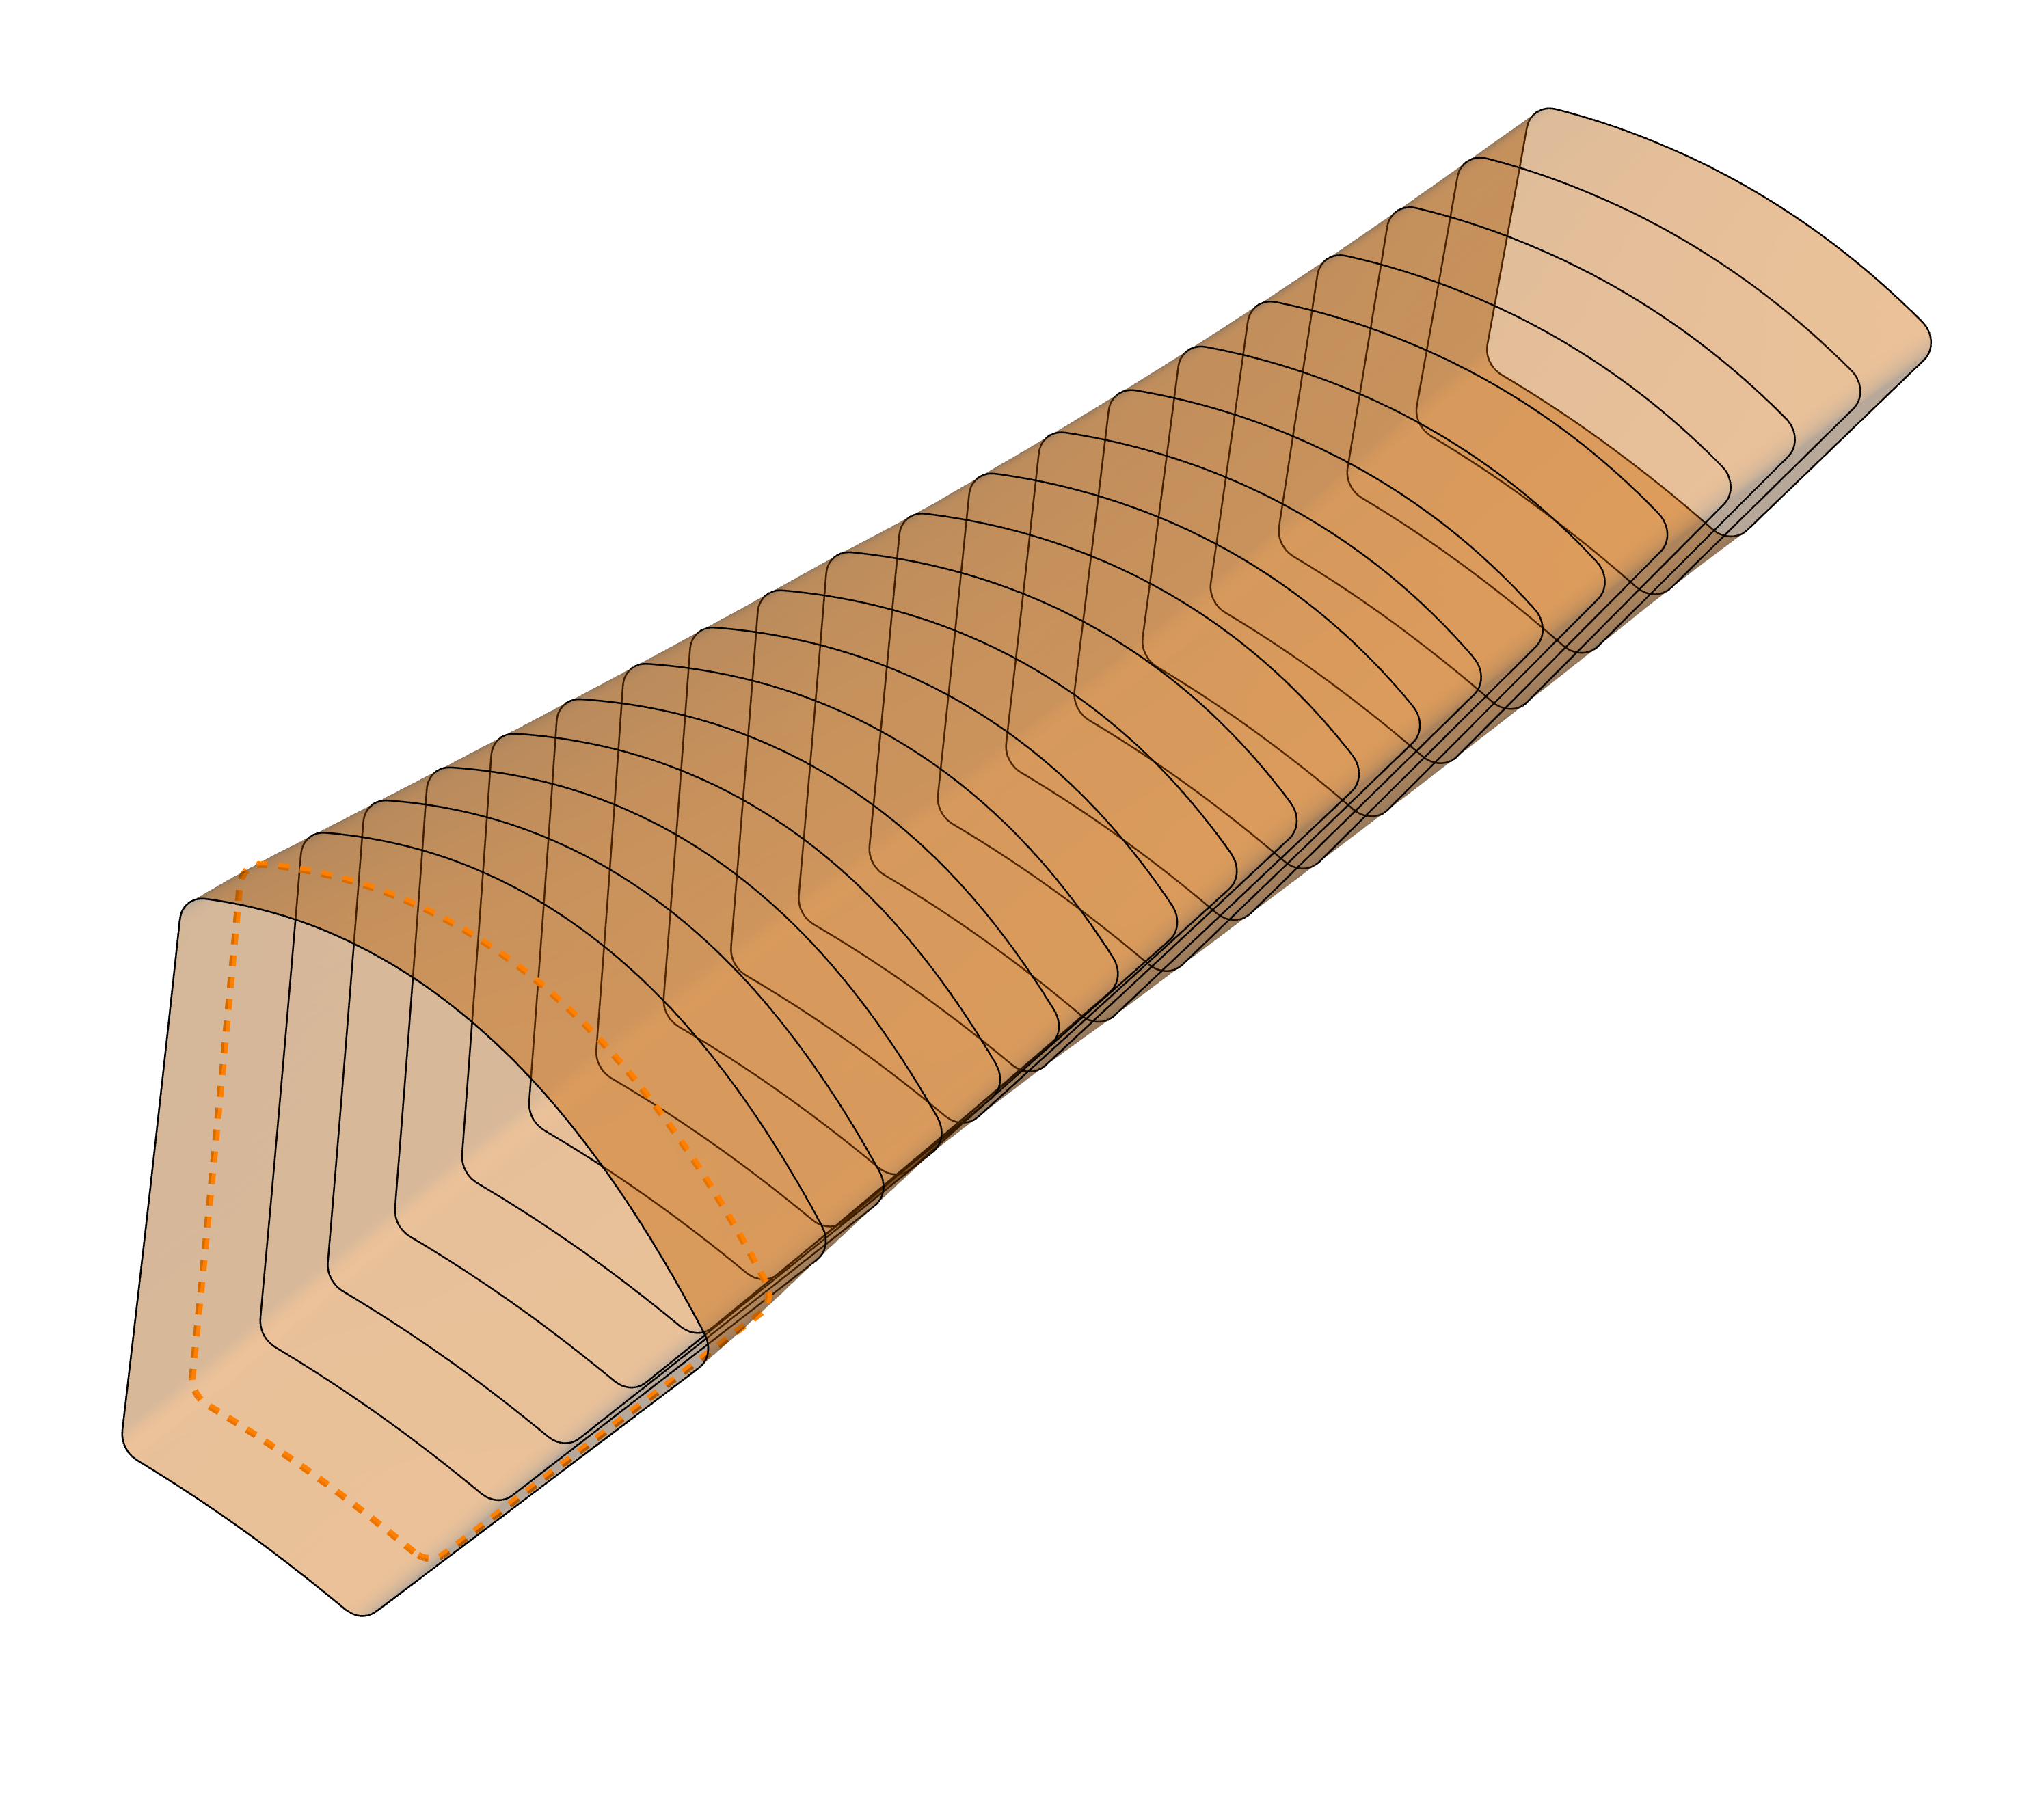
\includegraphics[width=\textwidth]{../../tec/chambers/114.png}
				\caption{Eine Kammer.}
			\end{subfigure}
			\begin{subfigure}{.36\textwidth}
				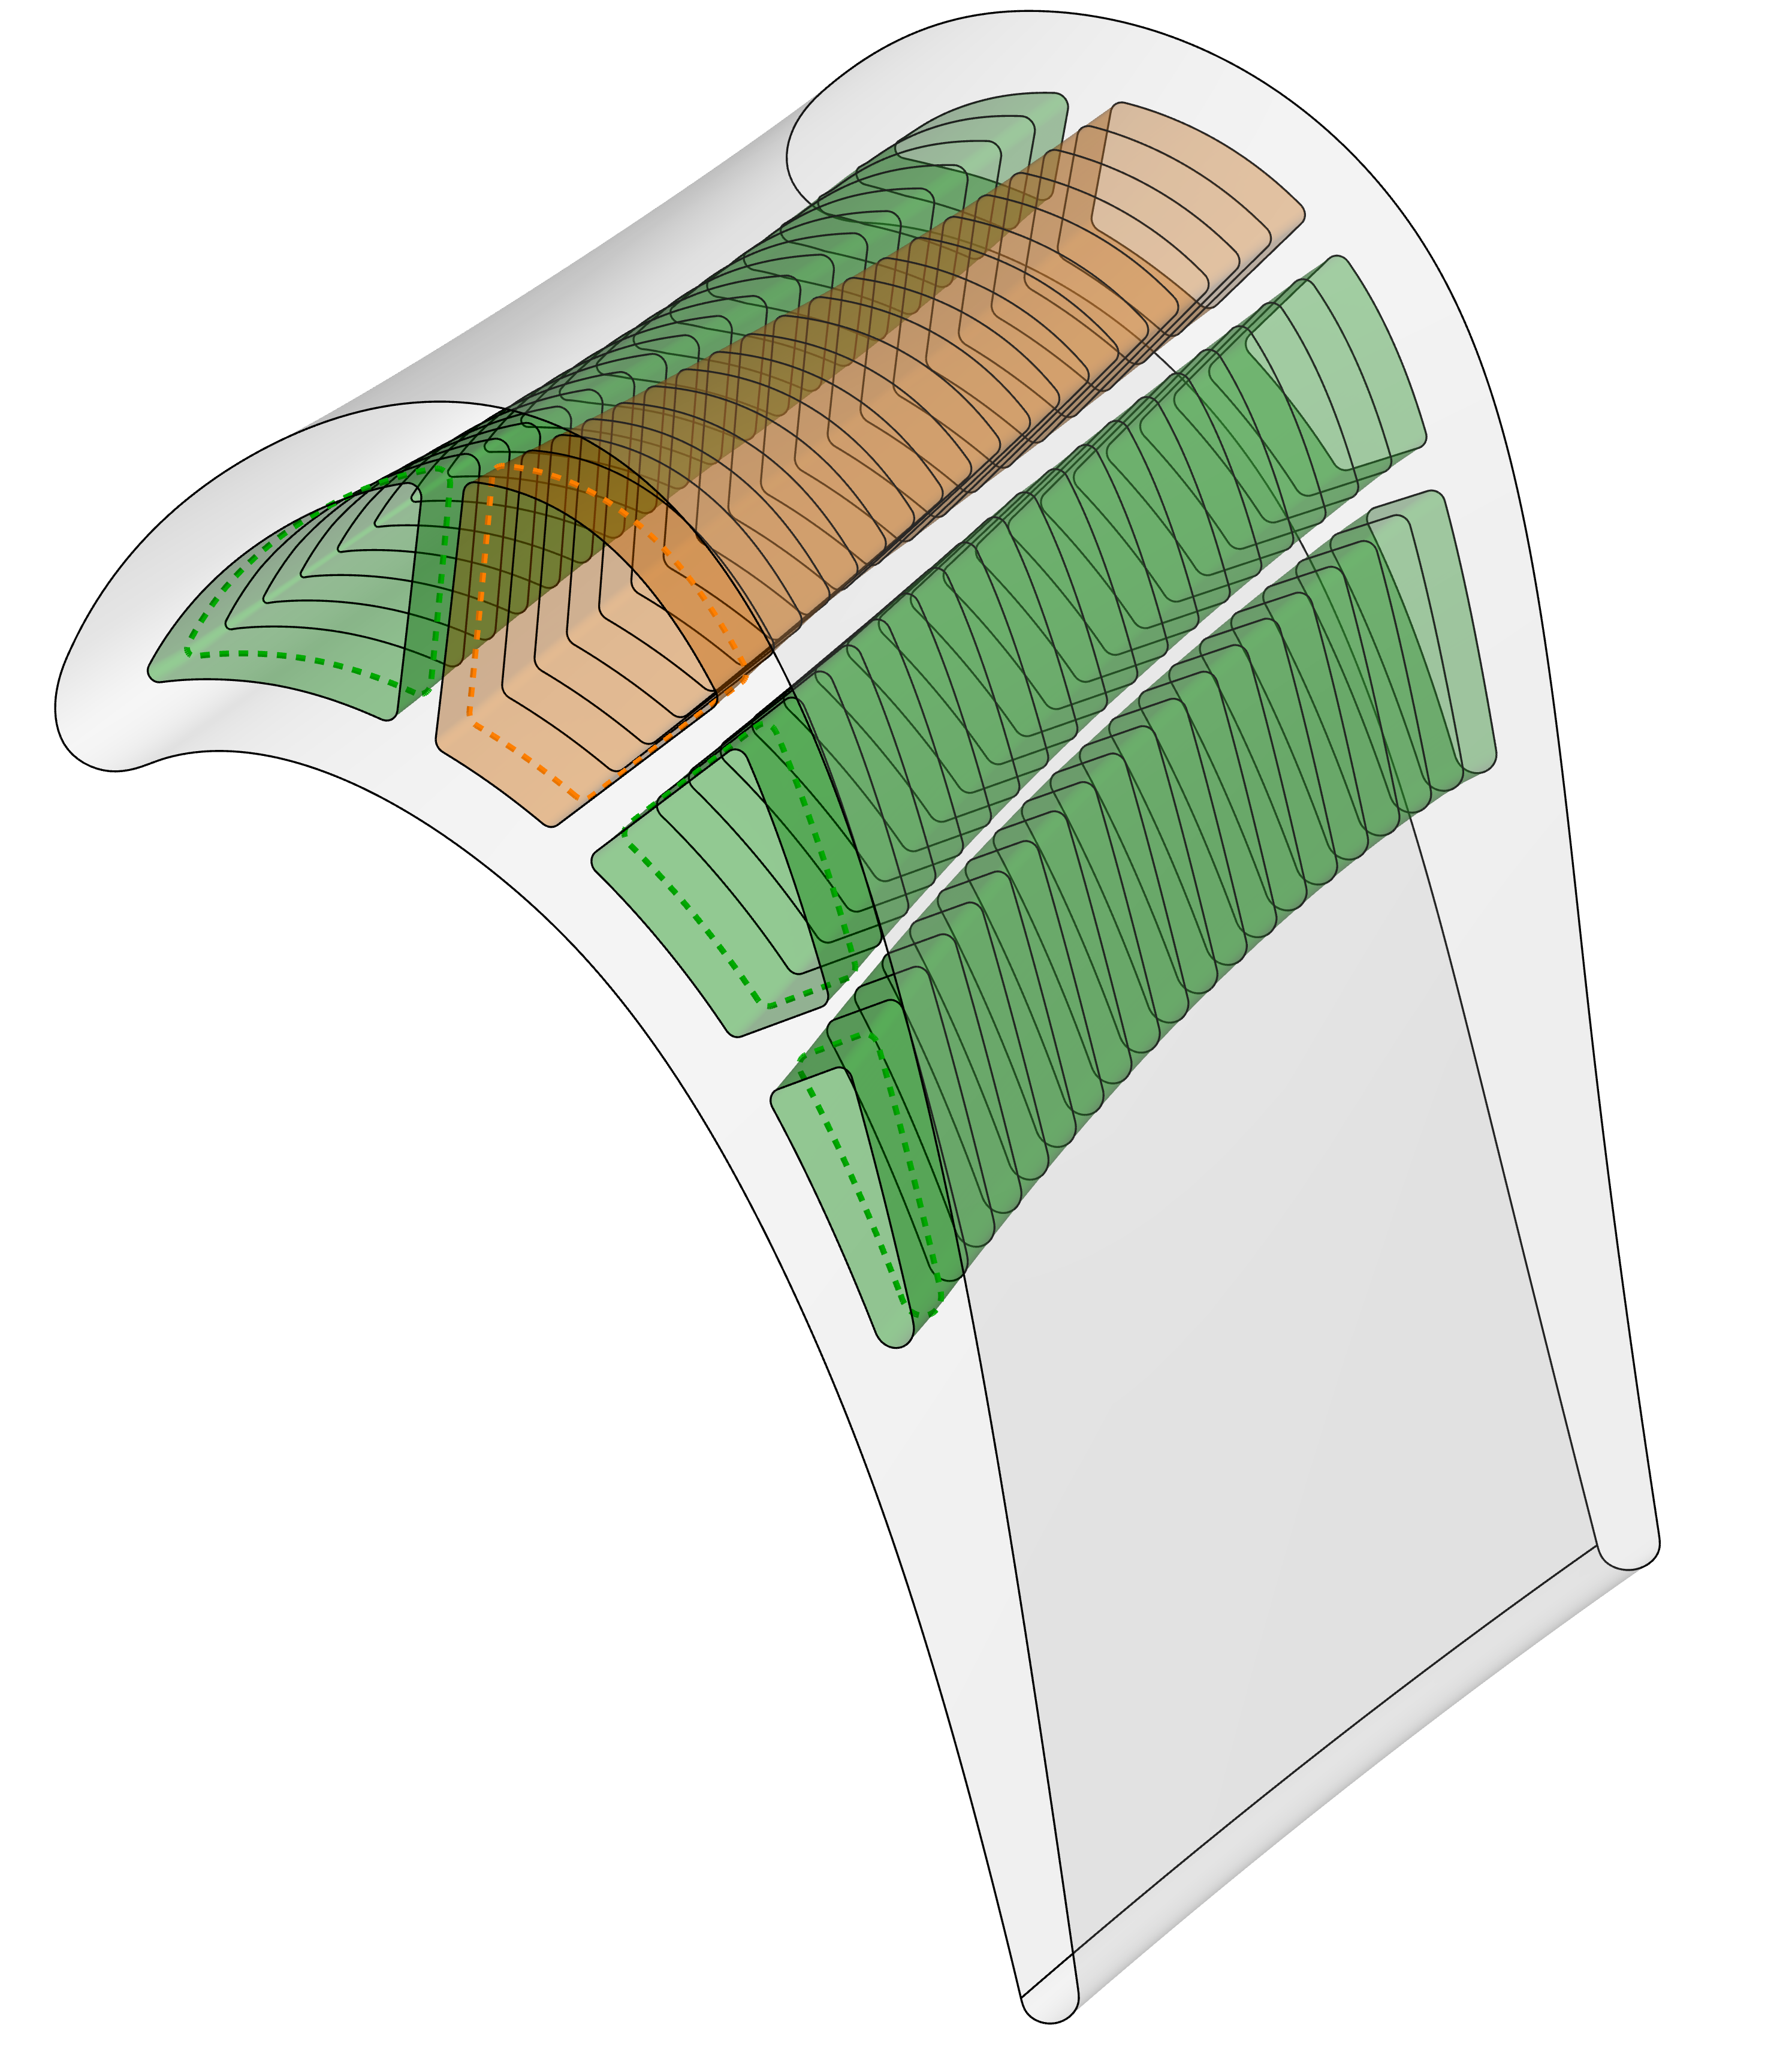
\includegraphics[width=\textwidth]{../../tec/chambers/111.png}
				\caption{Vier Kammern in der Schaufel.}
			\end{subfigure}
		\end{figure}
	\end{minipage}
	\vfill
\end{frame}

\begin{frame}
	\frametitle{Geometrien / Kanäle / Umkehrungen}
	\vspace{-0.25cm}\hspace{-0.5cm}
	\centering
	\begin{minipage}[t]{\textwidth}
		\textbf{Umkehrungen} werden aus den Kammern erstellt:
		\begin{figure}[H]
			\centering
			\begin{subfigure}{.55\textwidth}
				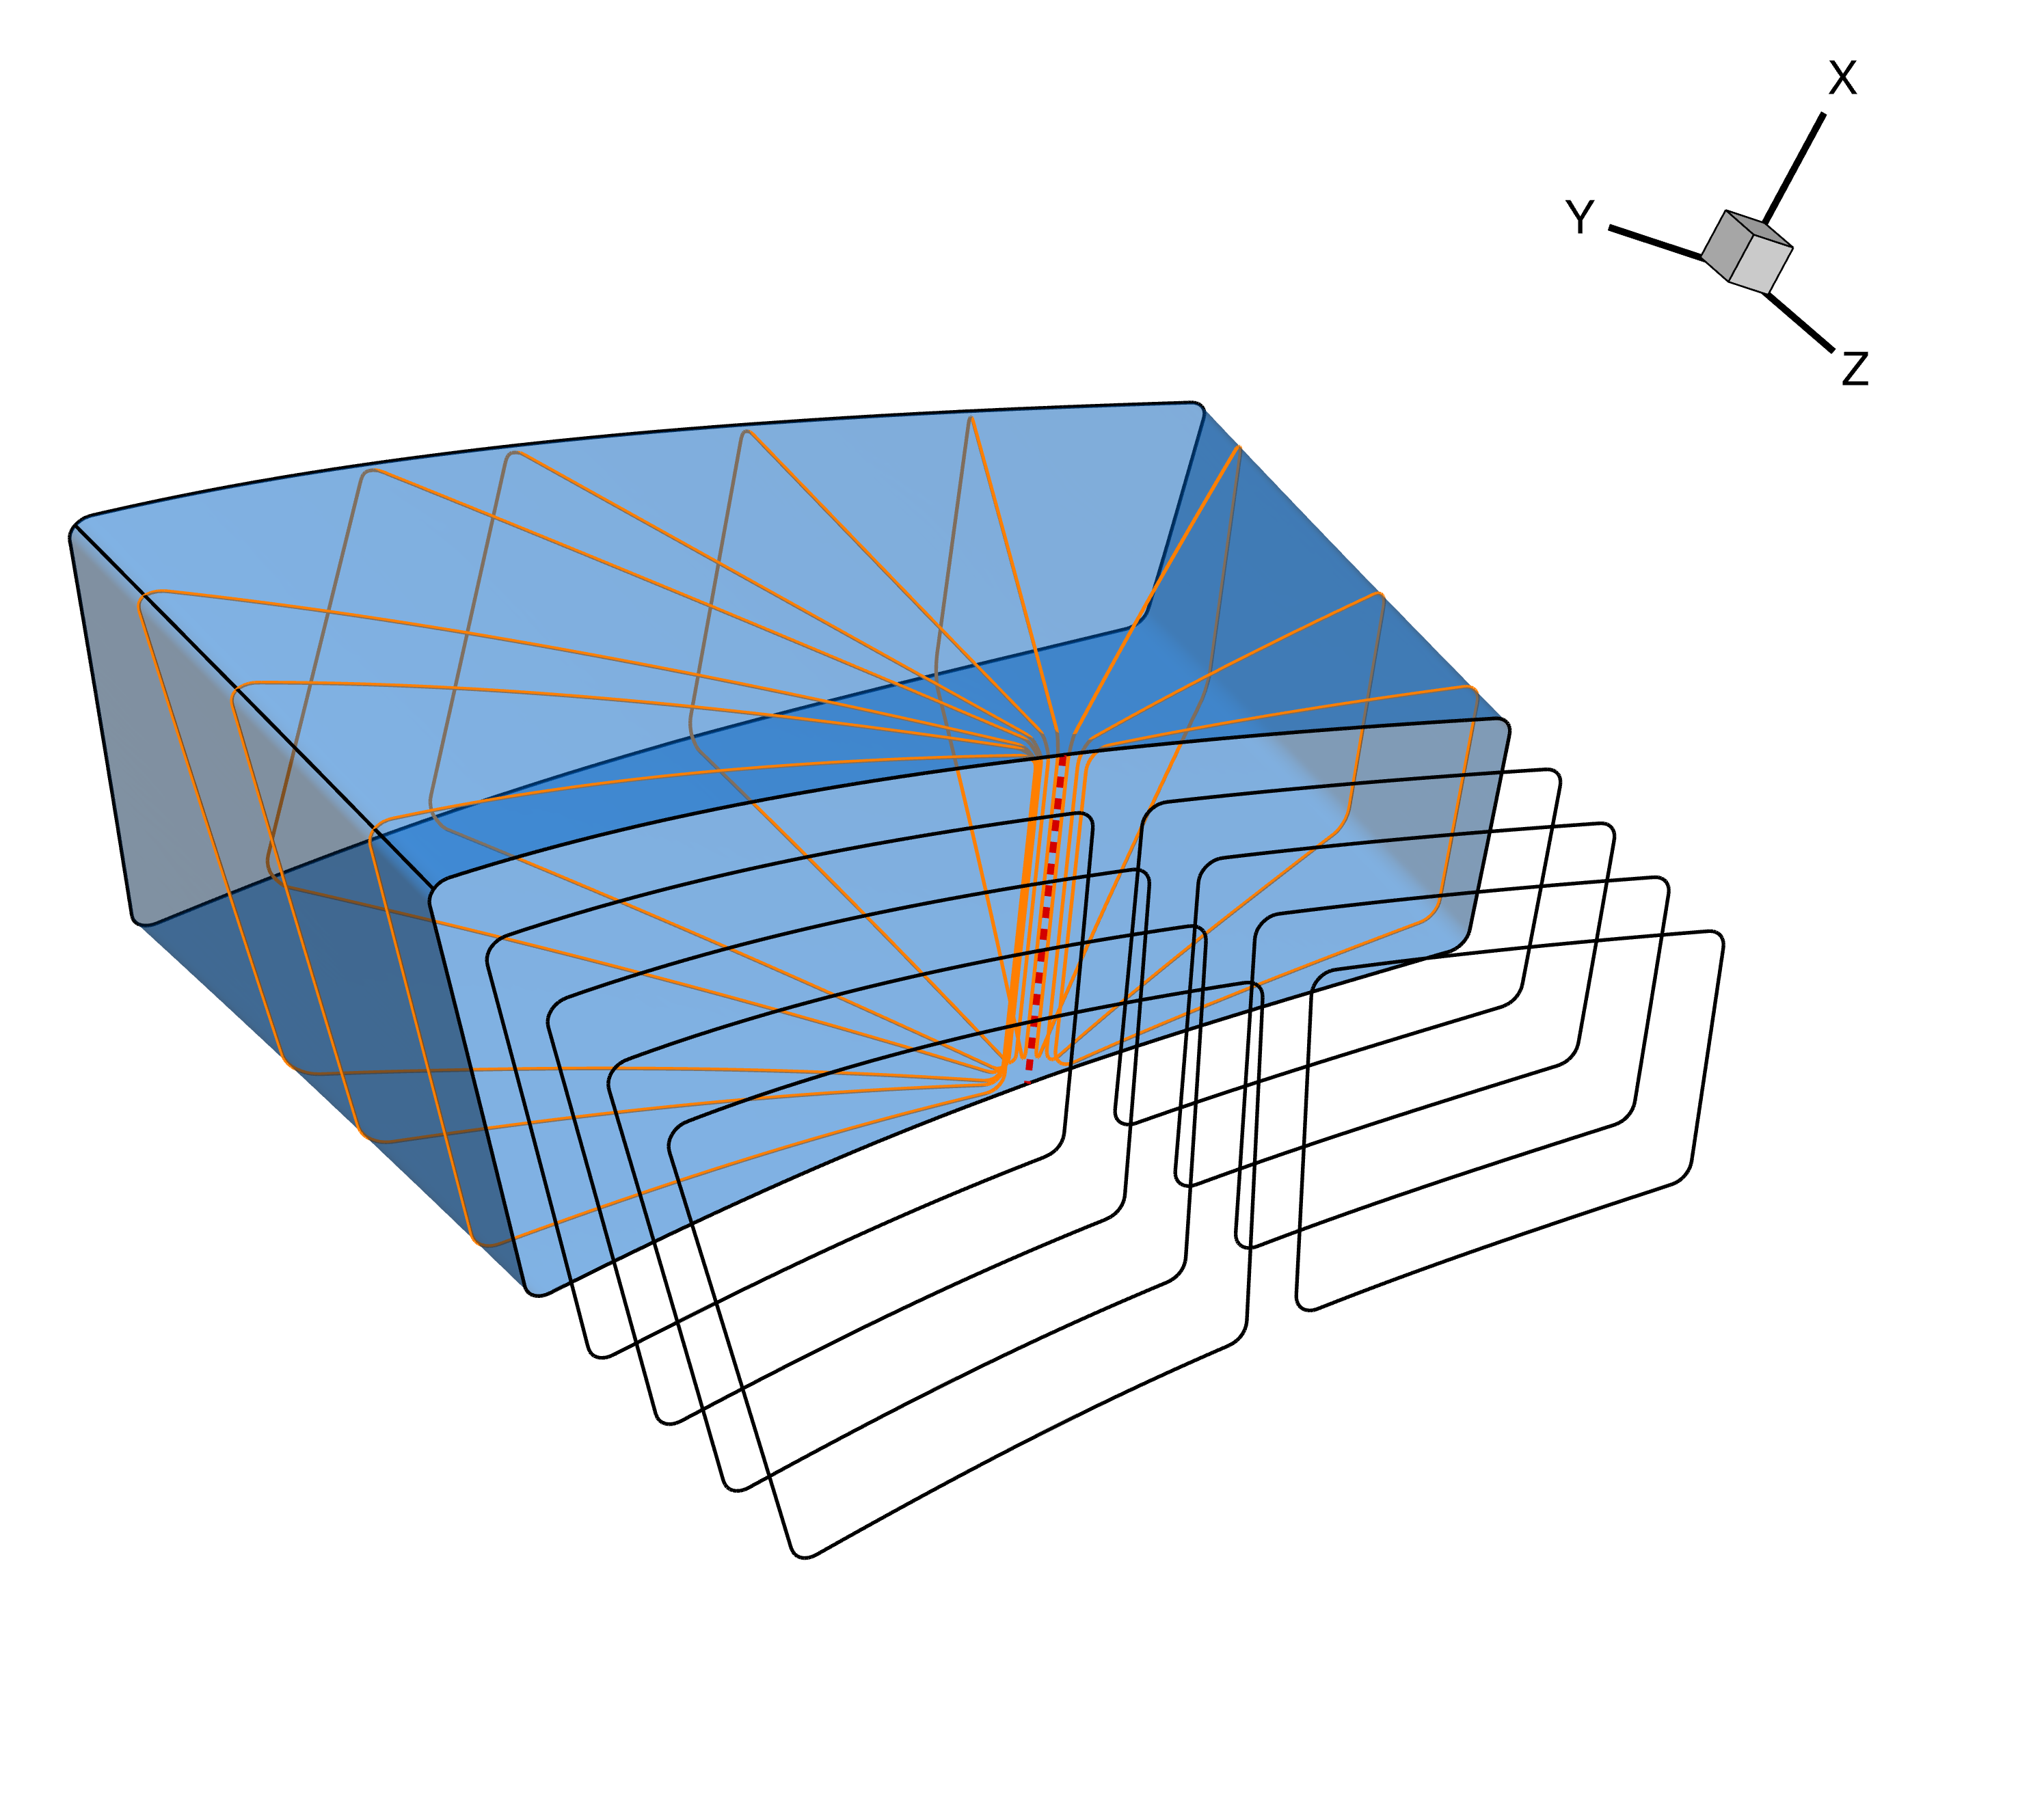
\includegraphics[width=\textwidth]{../../tec/channel/11.png}
			\end{subfigure}
			\begin{subfigure}{.32\textwidth}
				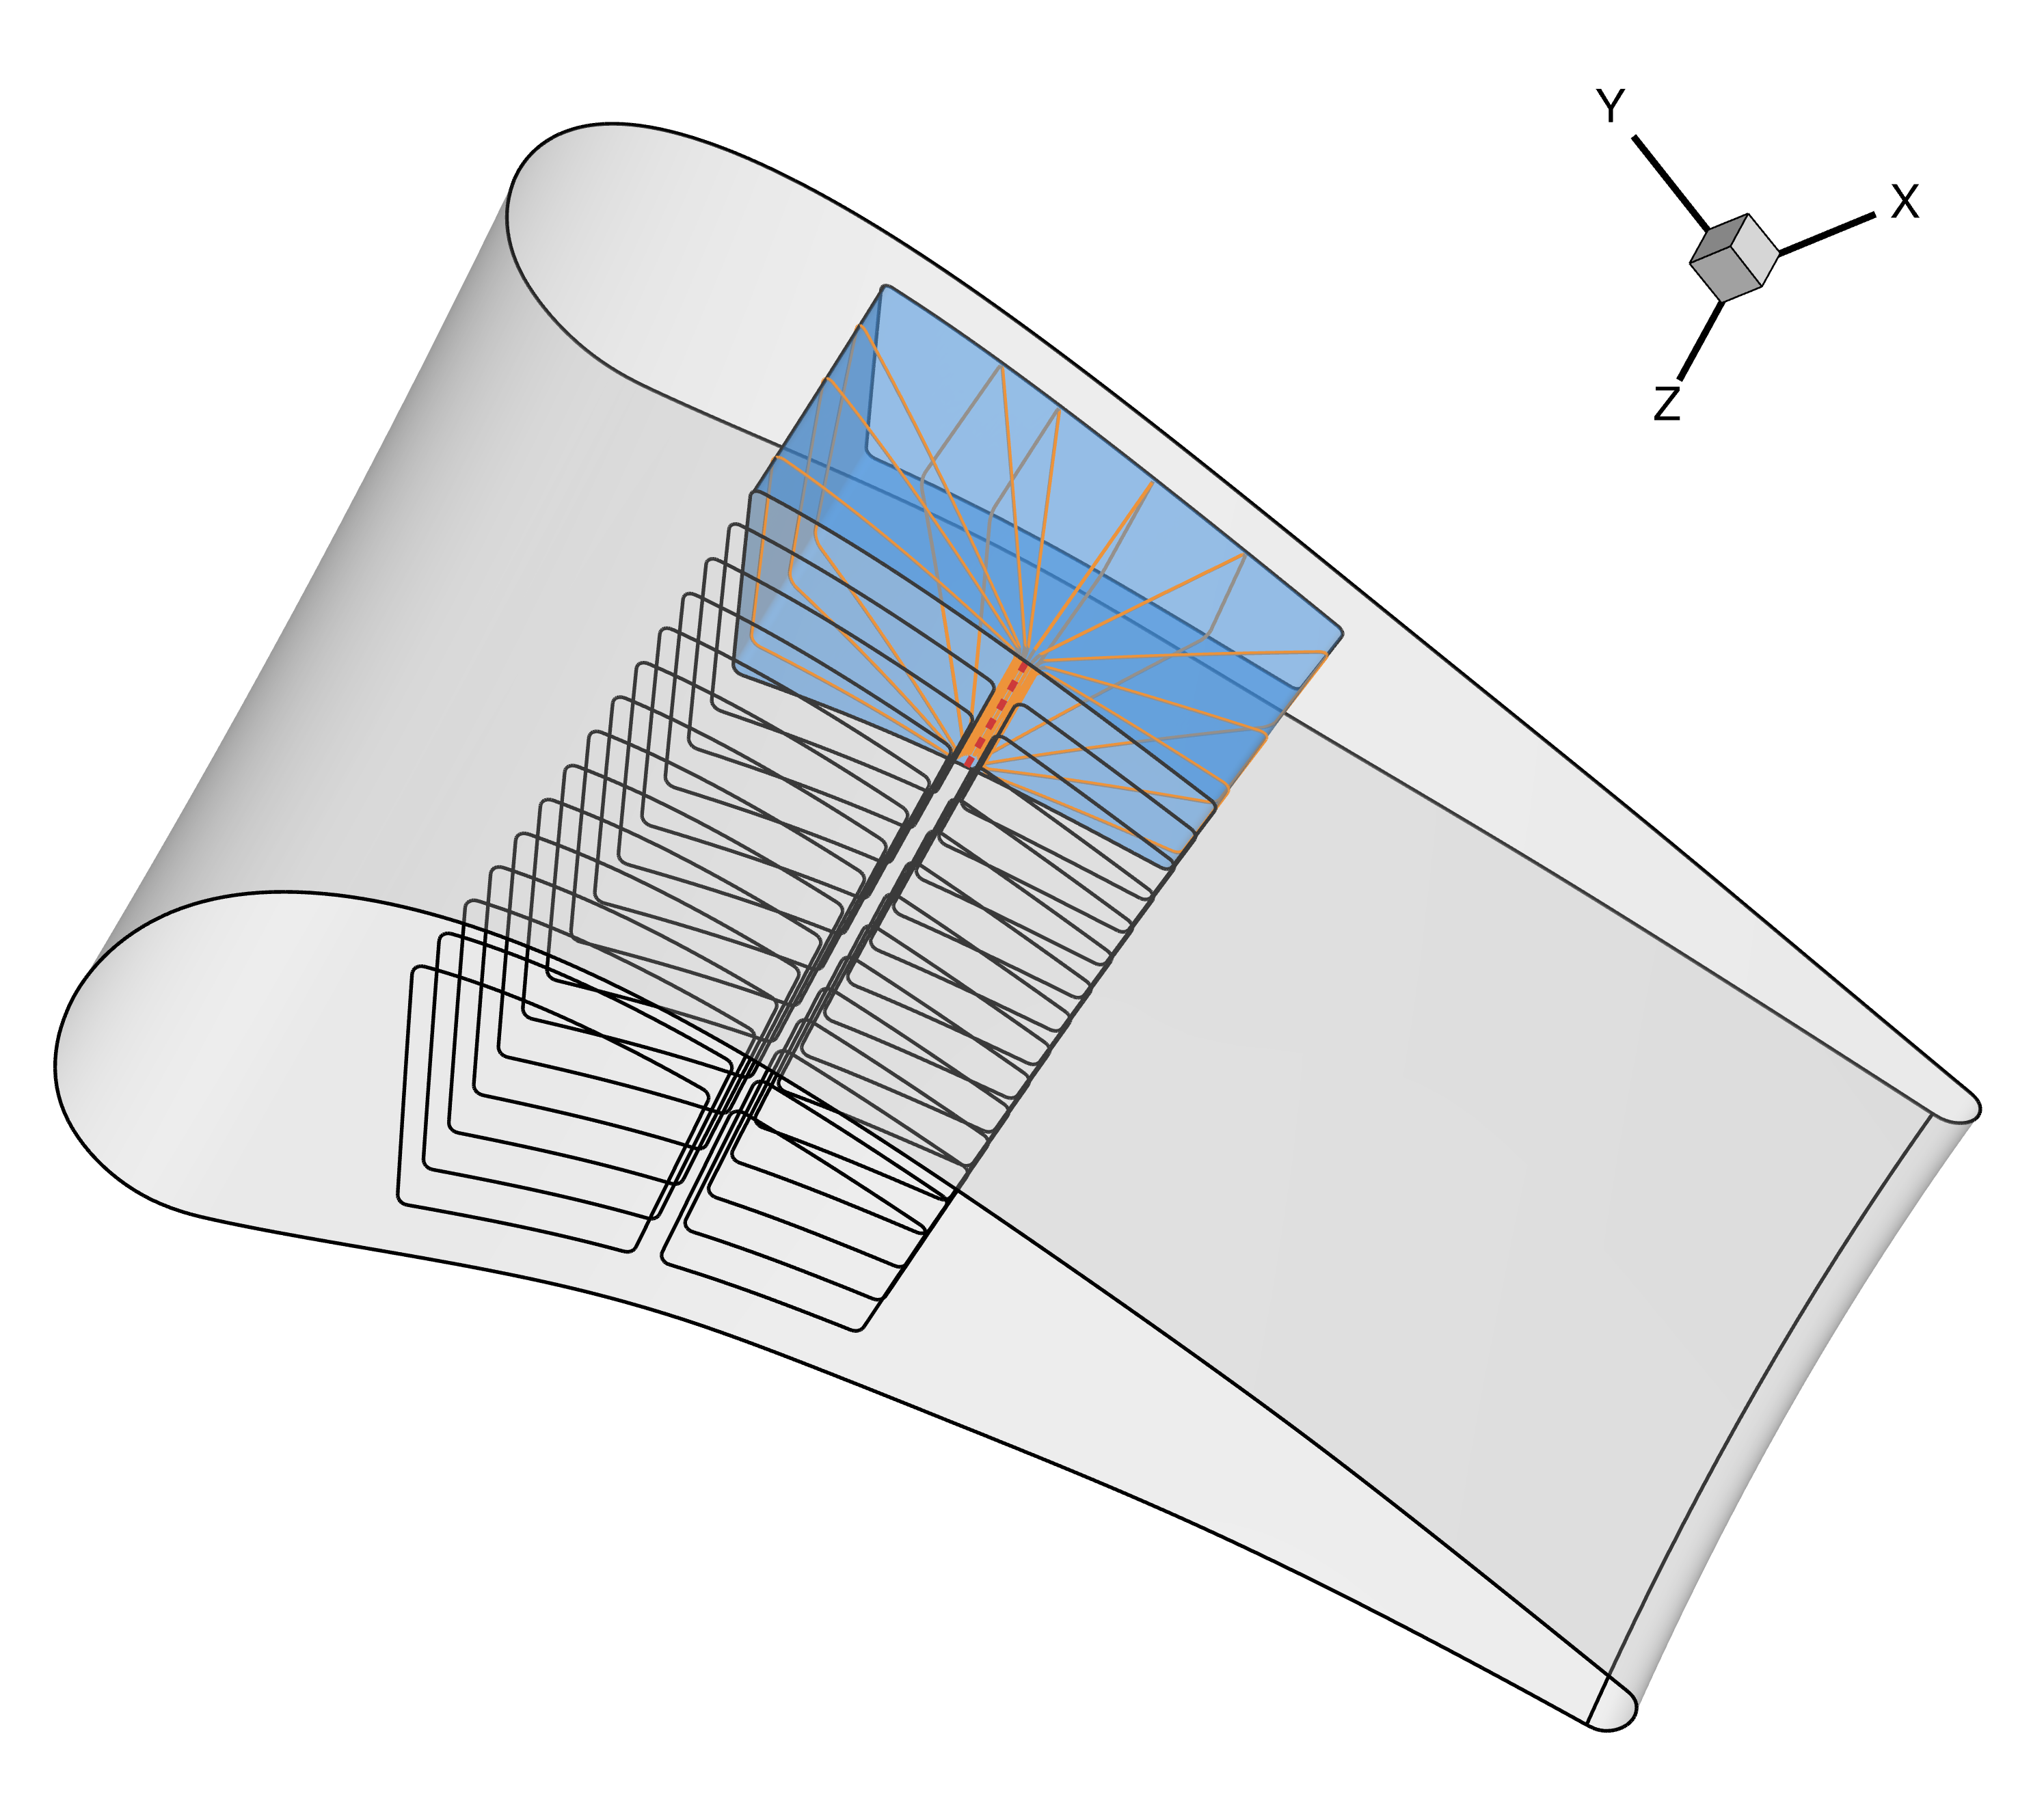
\includegraphics[width=\textwidth]{../../tec/channel/12.png}
				\vspace{1.2cm}
			\end{subfigure}
		\end{figure}
	\end{minipage}
	\vfill
\end{frame}

\begin{frame}
	\frametitle{Geometrien / Kanäle / Umkehrungen}
	\vspace{-0.5cm}\hspace{-0.5cm}
	\centering
	\begin{minipage}[t]{\textwidth}
		\begin{figure}[H]
			\centering
			\begin{subfigure}{.49\textwidth}
				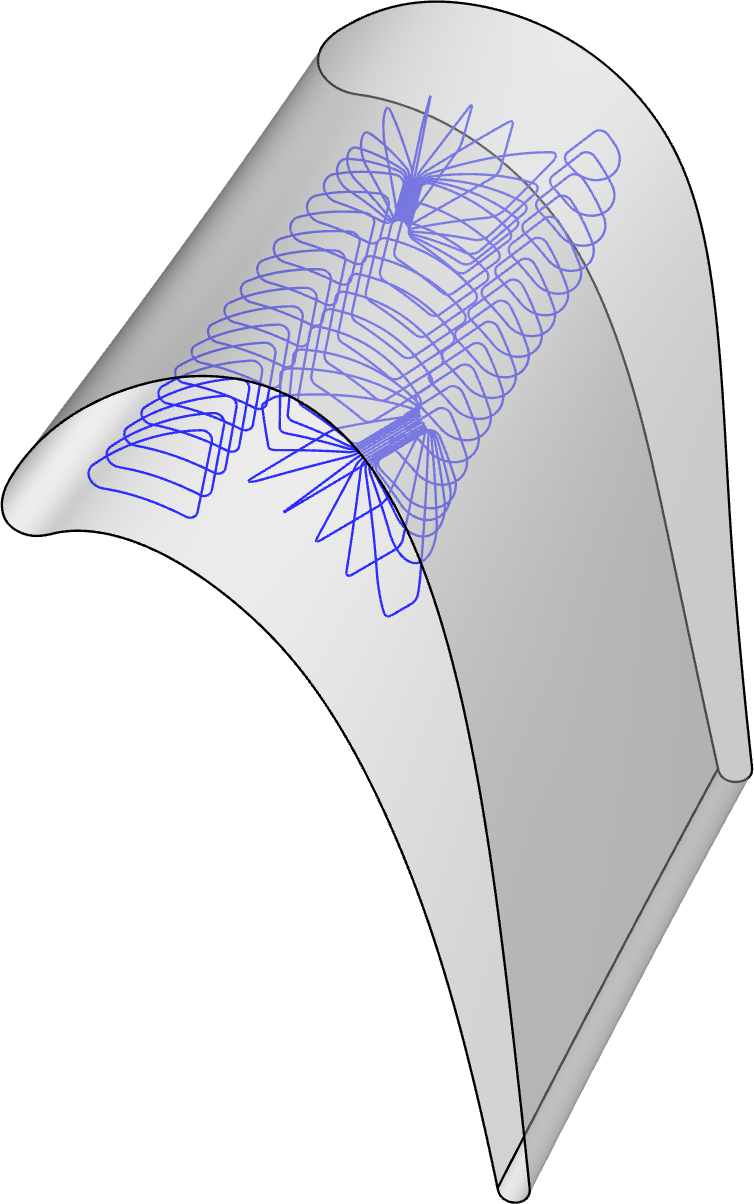
\includegraphics[width=\textwidth]{../../tec/channel/13.png}
			\end{subfigure}
			\begin{subfigure}{.49\textwidth}
				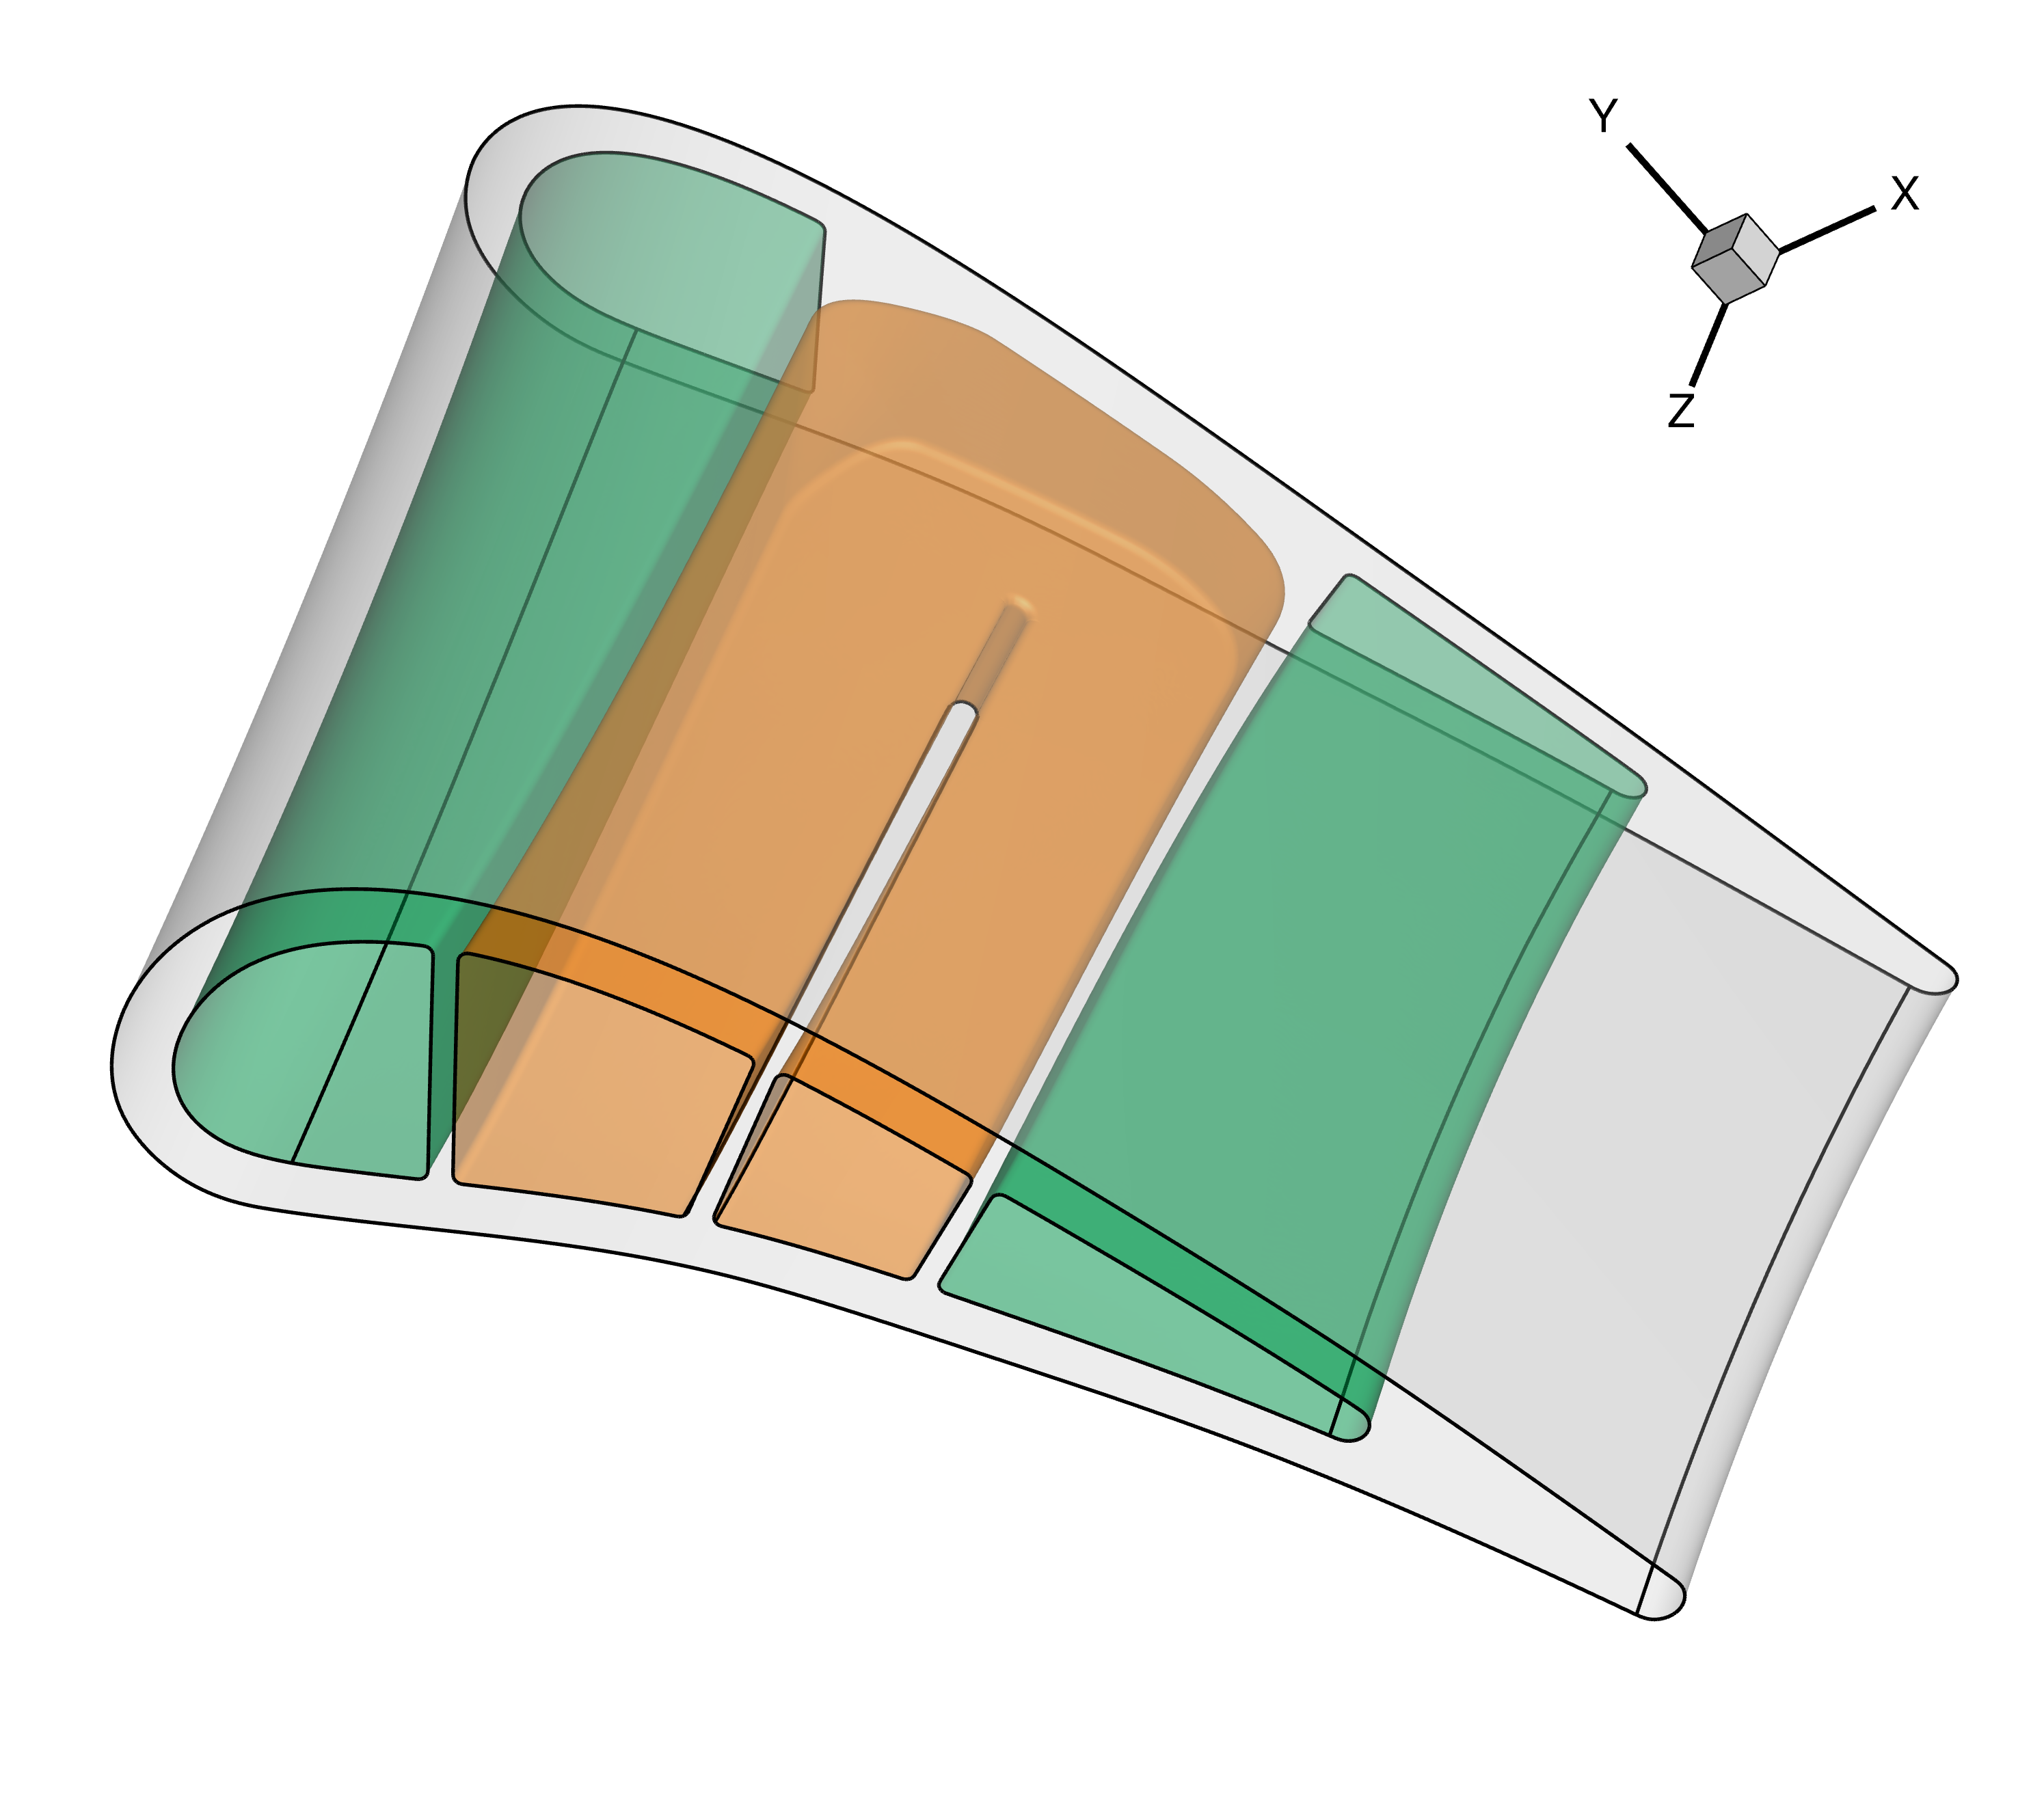
\includegraphics[width=\textwidth]{../../tec/channel/14.png}
			\end{subfigure}
		\end{figure}
	\end{minipage}
	\vfill
\end{frame}

\begin{frame}
	\frametitle{Geometrien / Kanäle}
	\vspace{-0.25cm}\hspace{-0.5cm}
	Kammern und Umkehrungen \textrightarrow{} \textbf{Kanäle}
	\centering
	\begin{minipage}[t]{.8\textwidth}
		\begin{figure}[H]
			\centering
			\begin{subfigure}{.49\textwidth}
				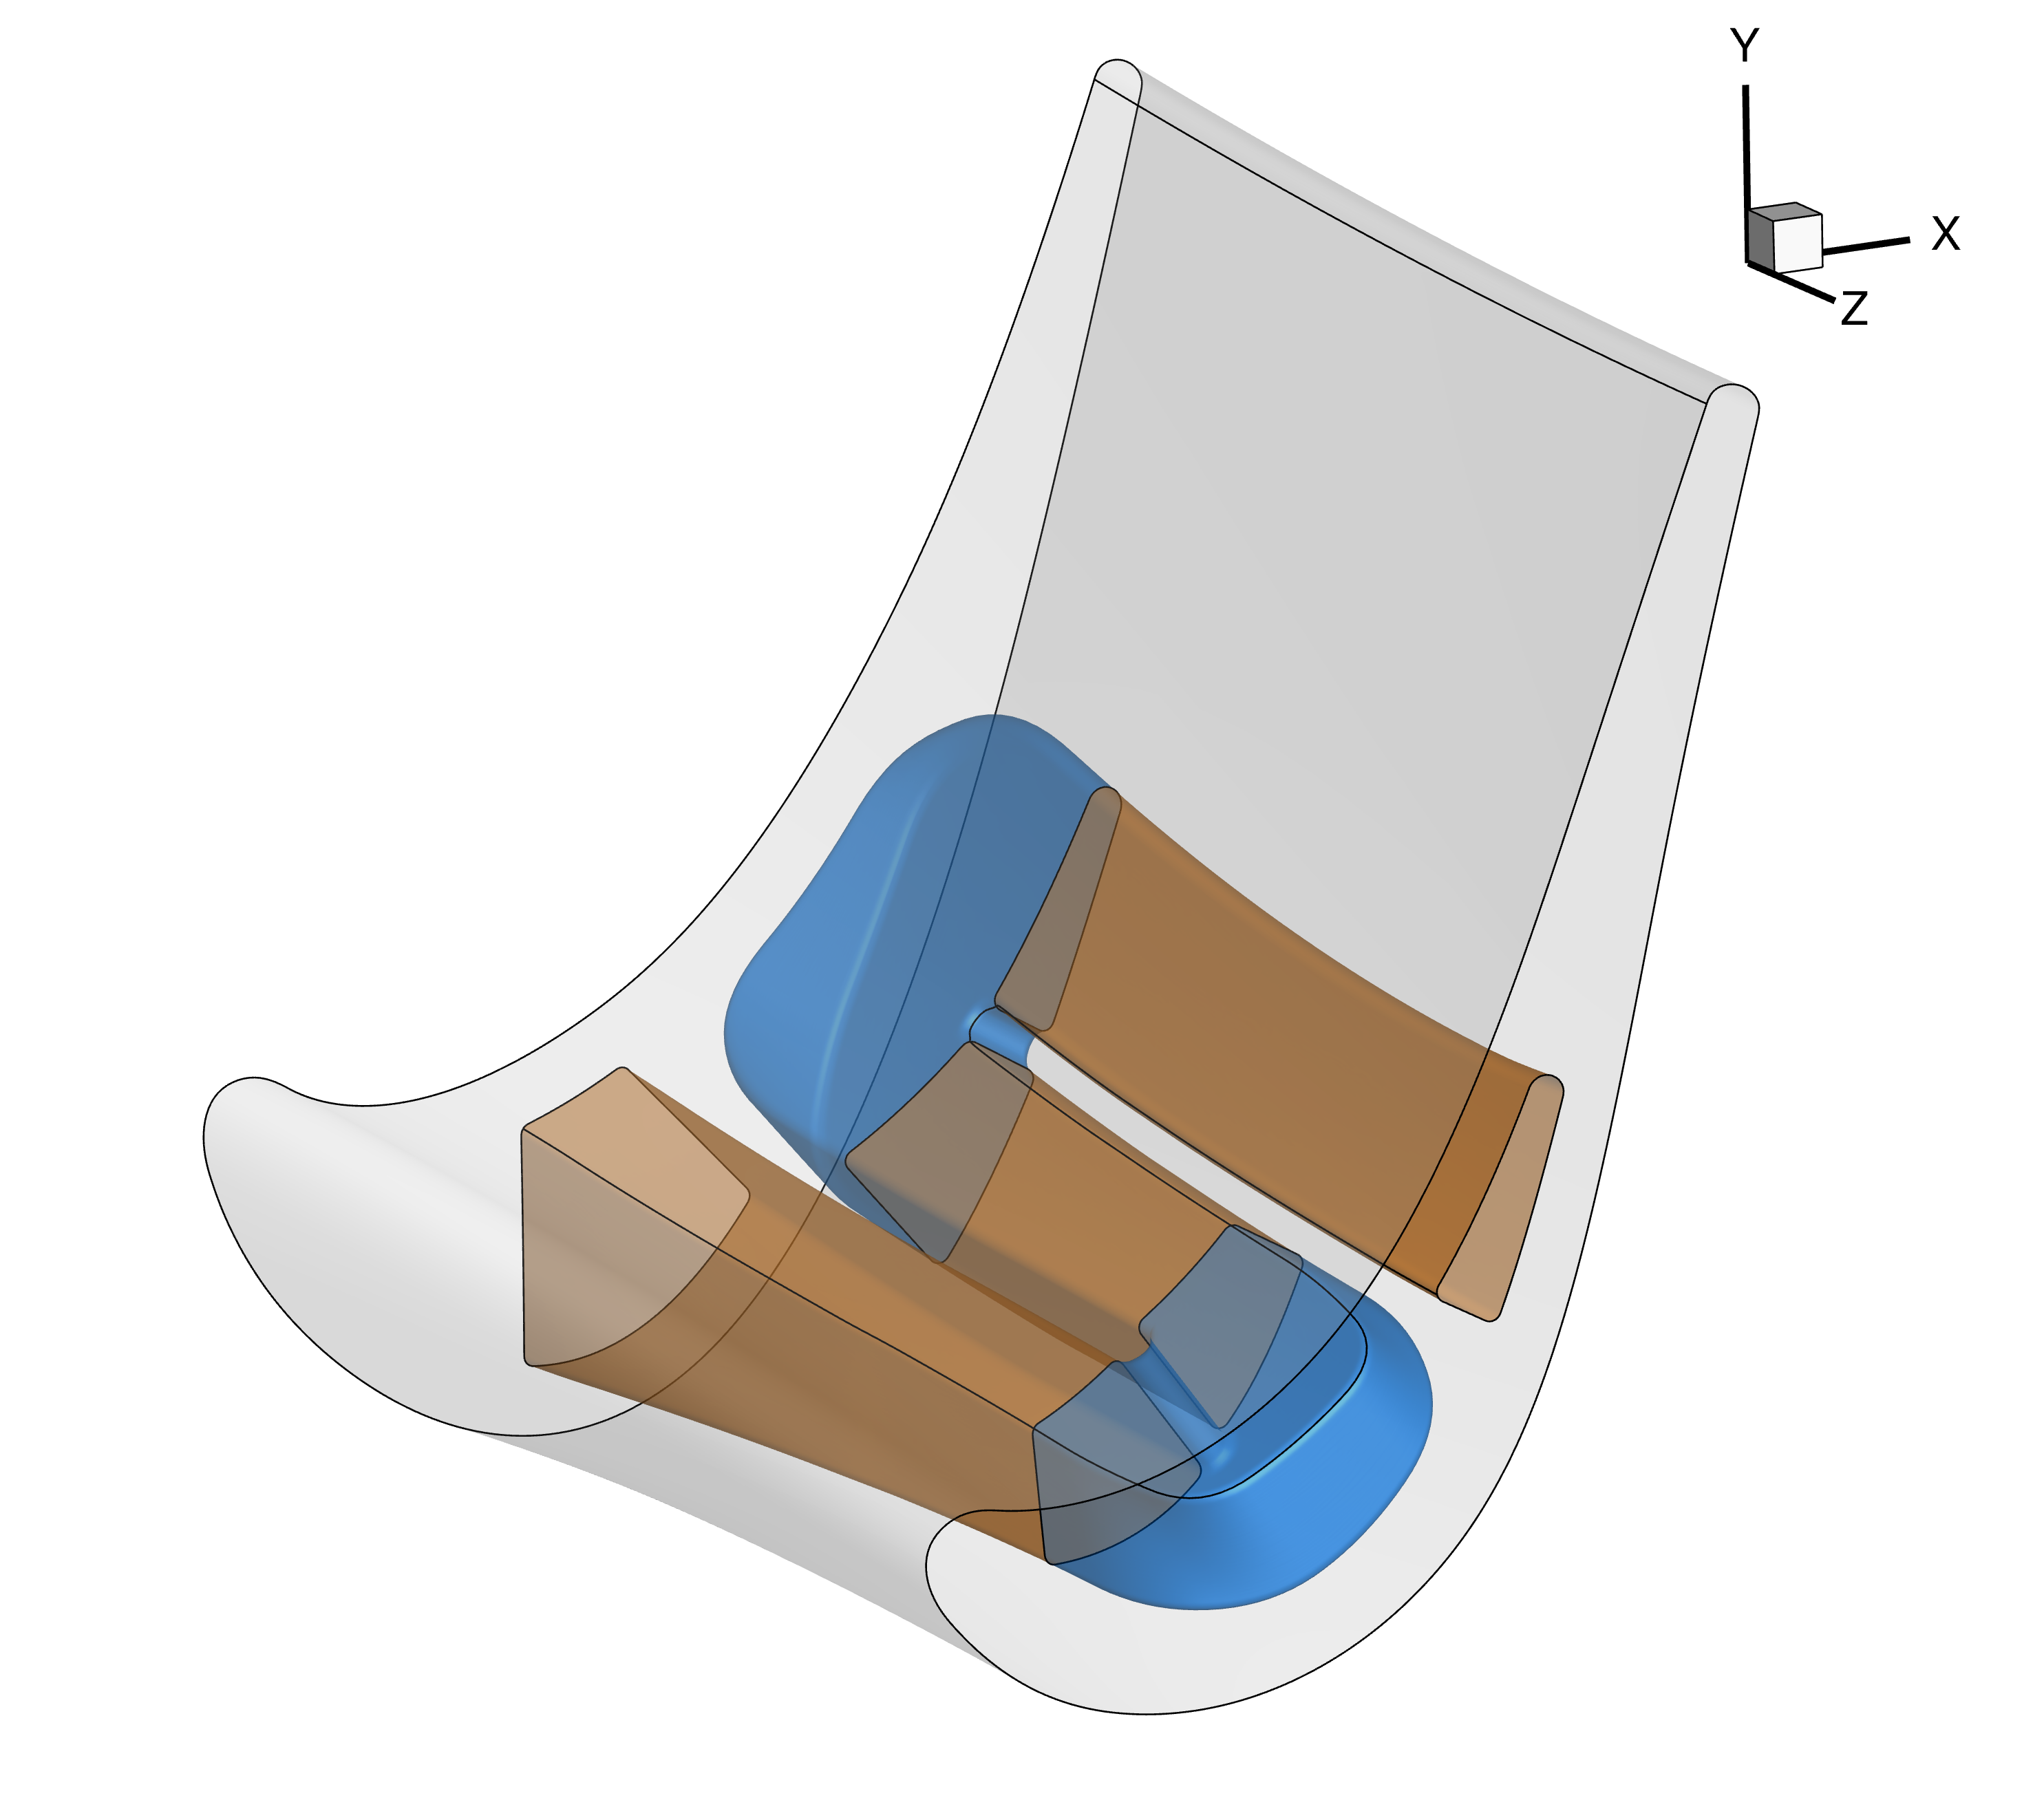
\includegraphics[width=\textwidth]{../../tec/complete/020.png}
			\end{subfigure}
			\begin{subfigure}{.49\textwidth}
				\centering
				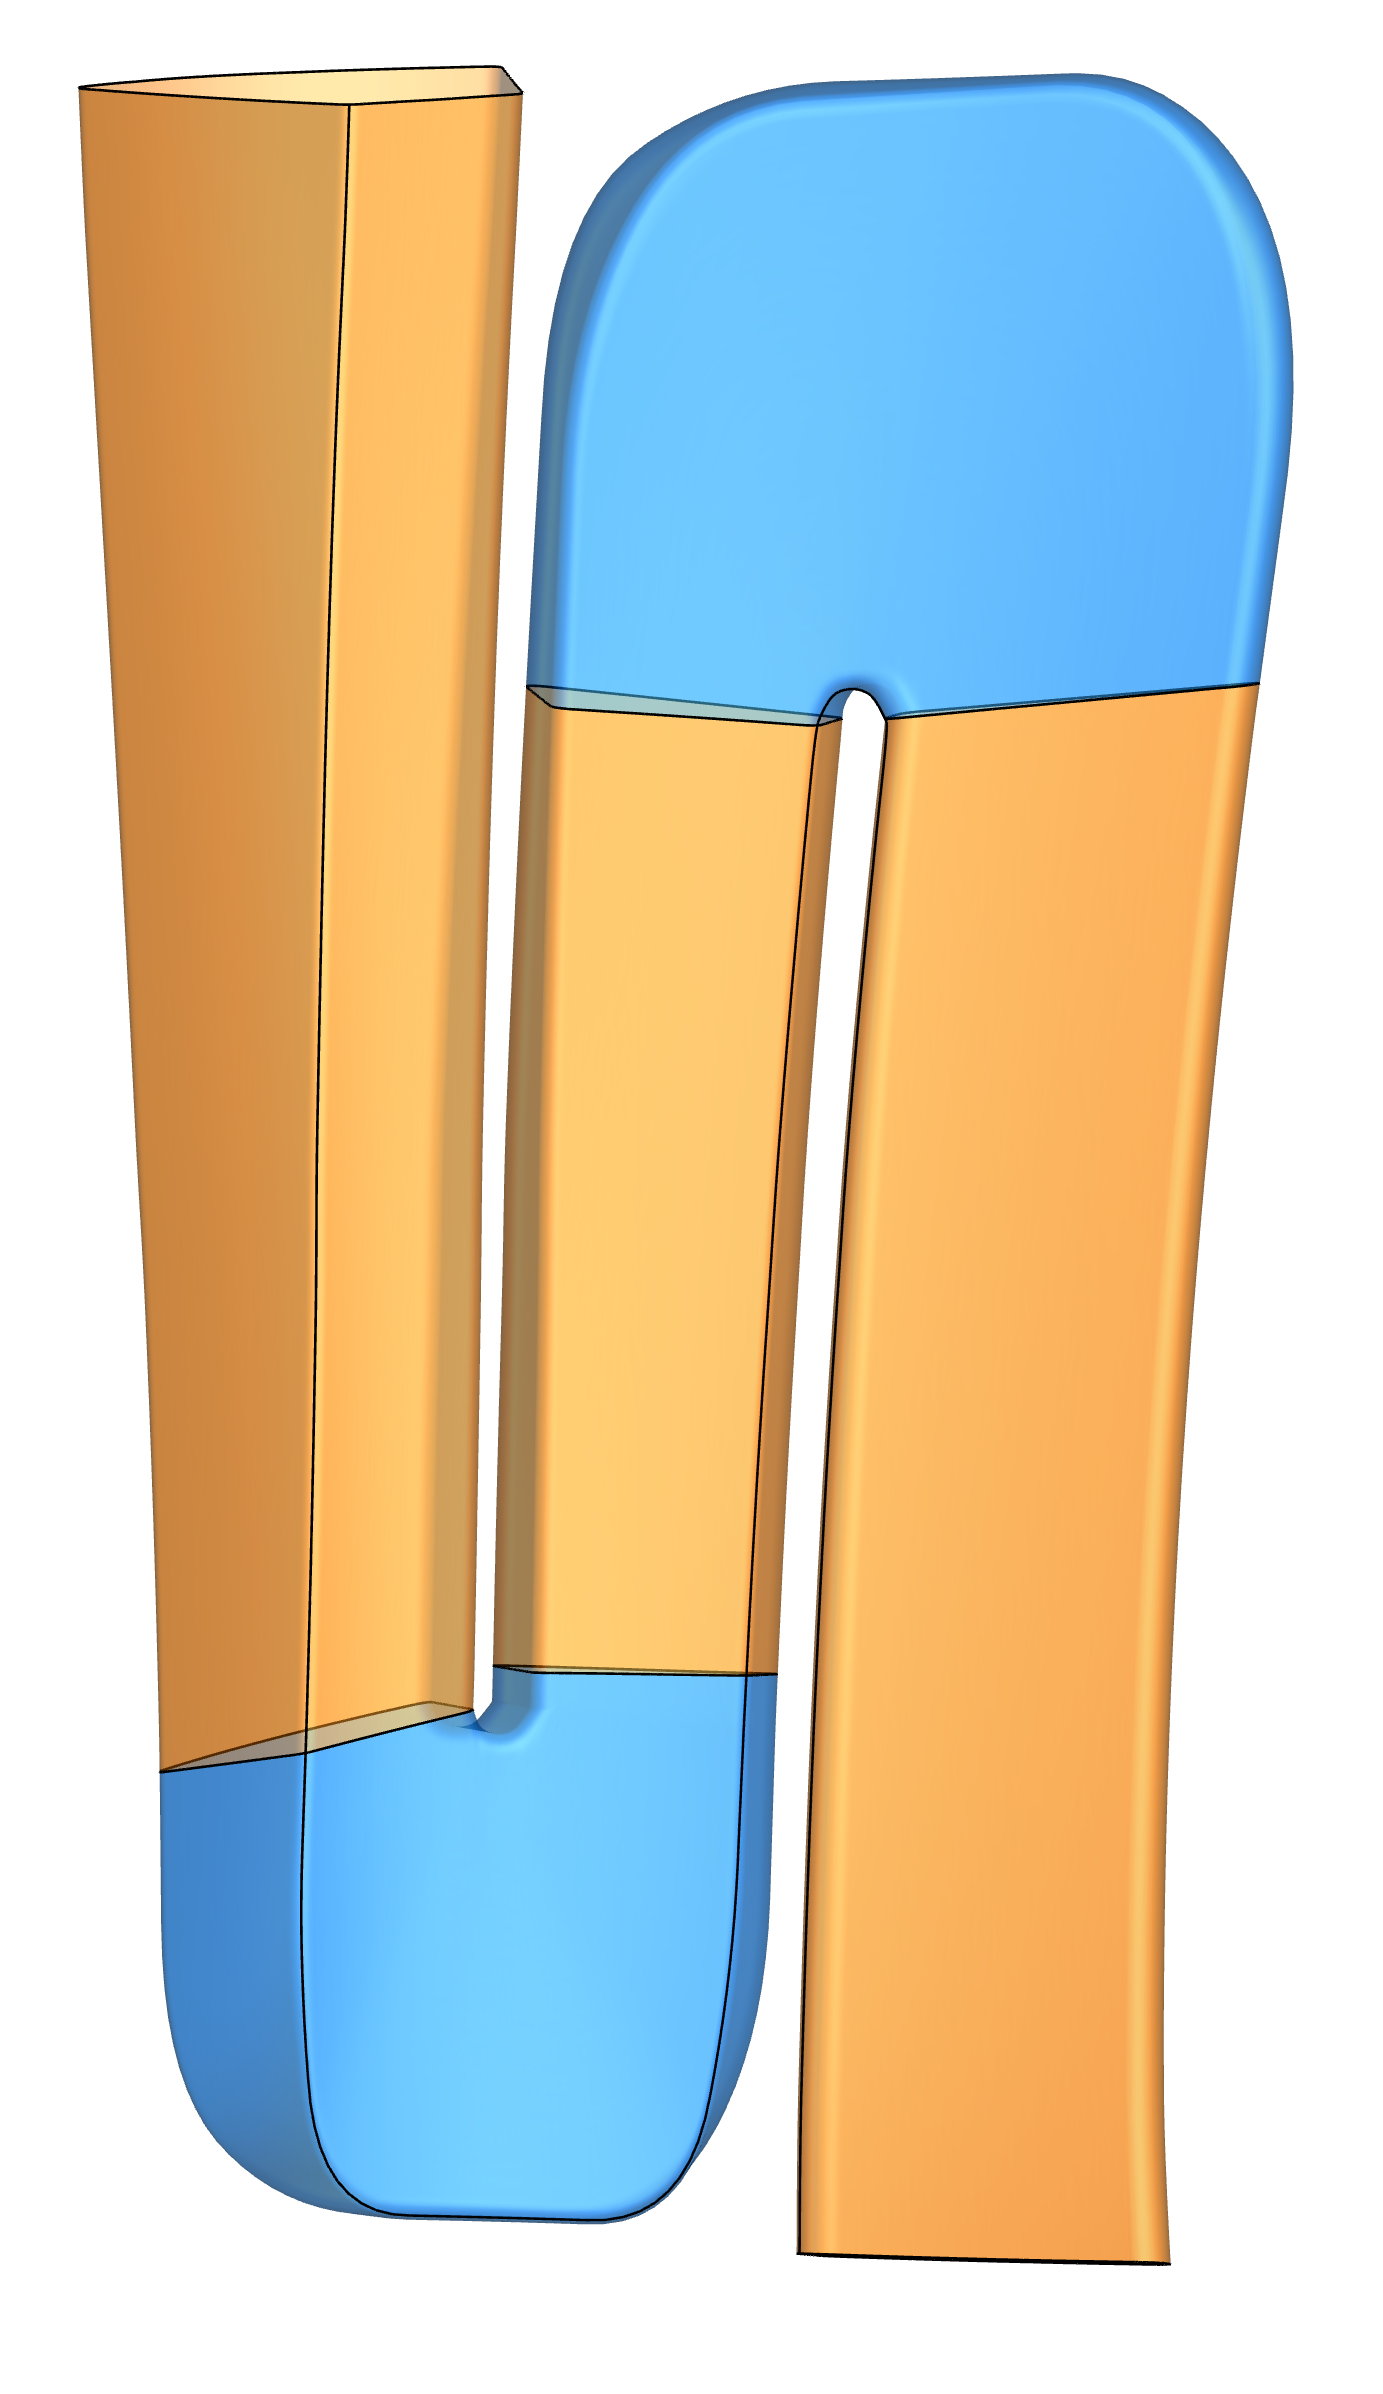
\includegraphics[width=.5\textwidth]{../../tec/complete/021.png}
			\end{subfigure}
		\end{figure}
	\end{minipage}
	\vfill
\end{frame}

\begin{frame}
	\frametitle{Geometrien / Überblick}
	\vspace{-1.5cm}\hspace{-0.5cm}
	\begin{minipage}[t]{0.38\textwidth}
		\begin{itemize}
			\item[\ding{108}] Kühlkanäle
			\item[\ding{109}] Filmkühlung
			\item[\ding{109}] Prallkühlung
			\item[\ding{109}] Ausblasungsschlitze
			\item[\ding{109}] Pin-fins
		\end{itemize}
	\end{minipage}
	\begin{minipage}{0.6\textwidth}
		\begin{figure}[H]
			\centering
			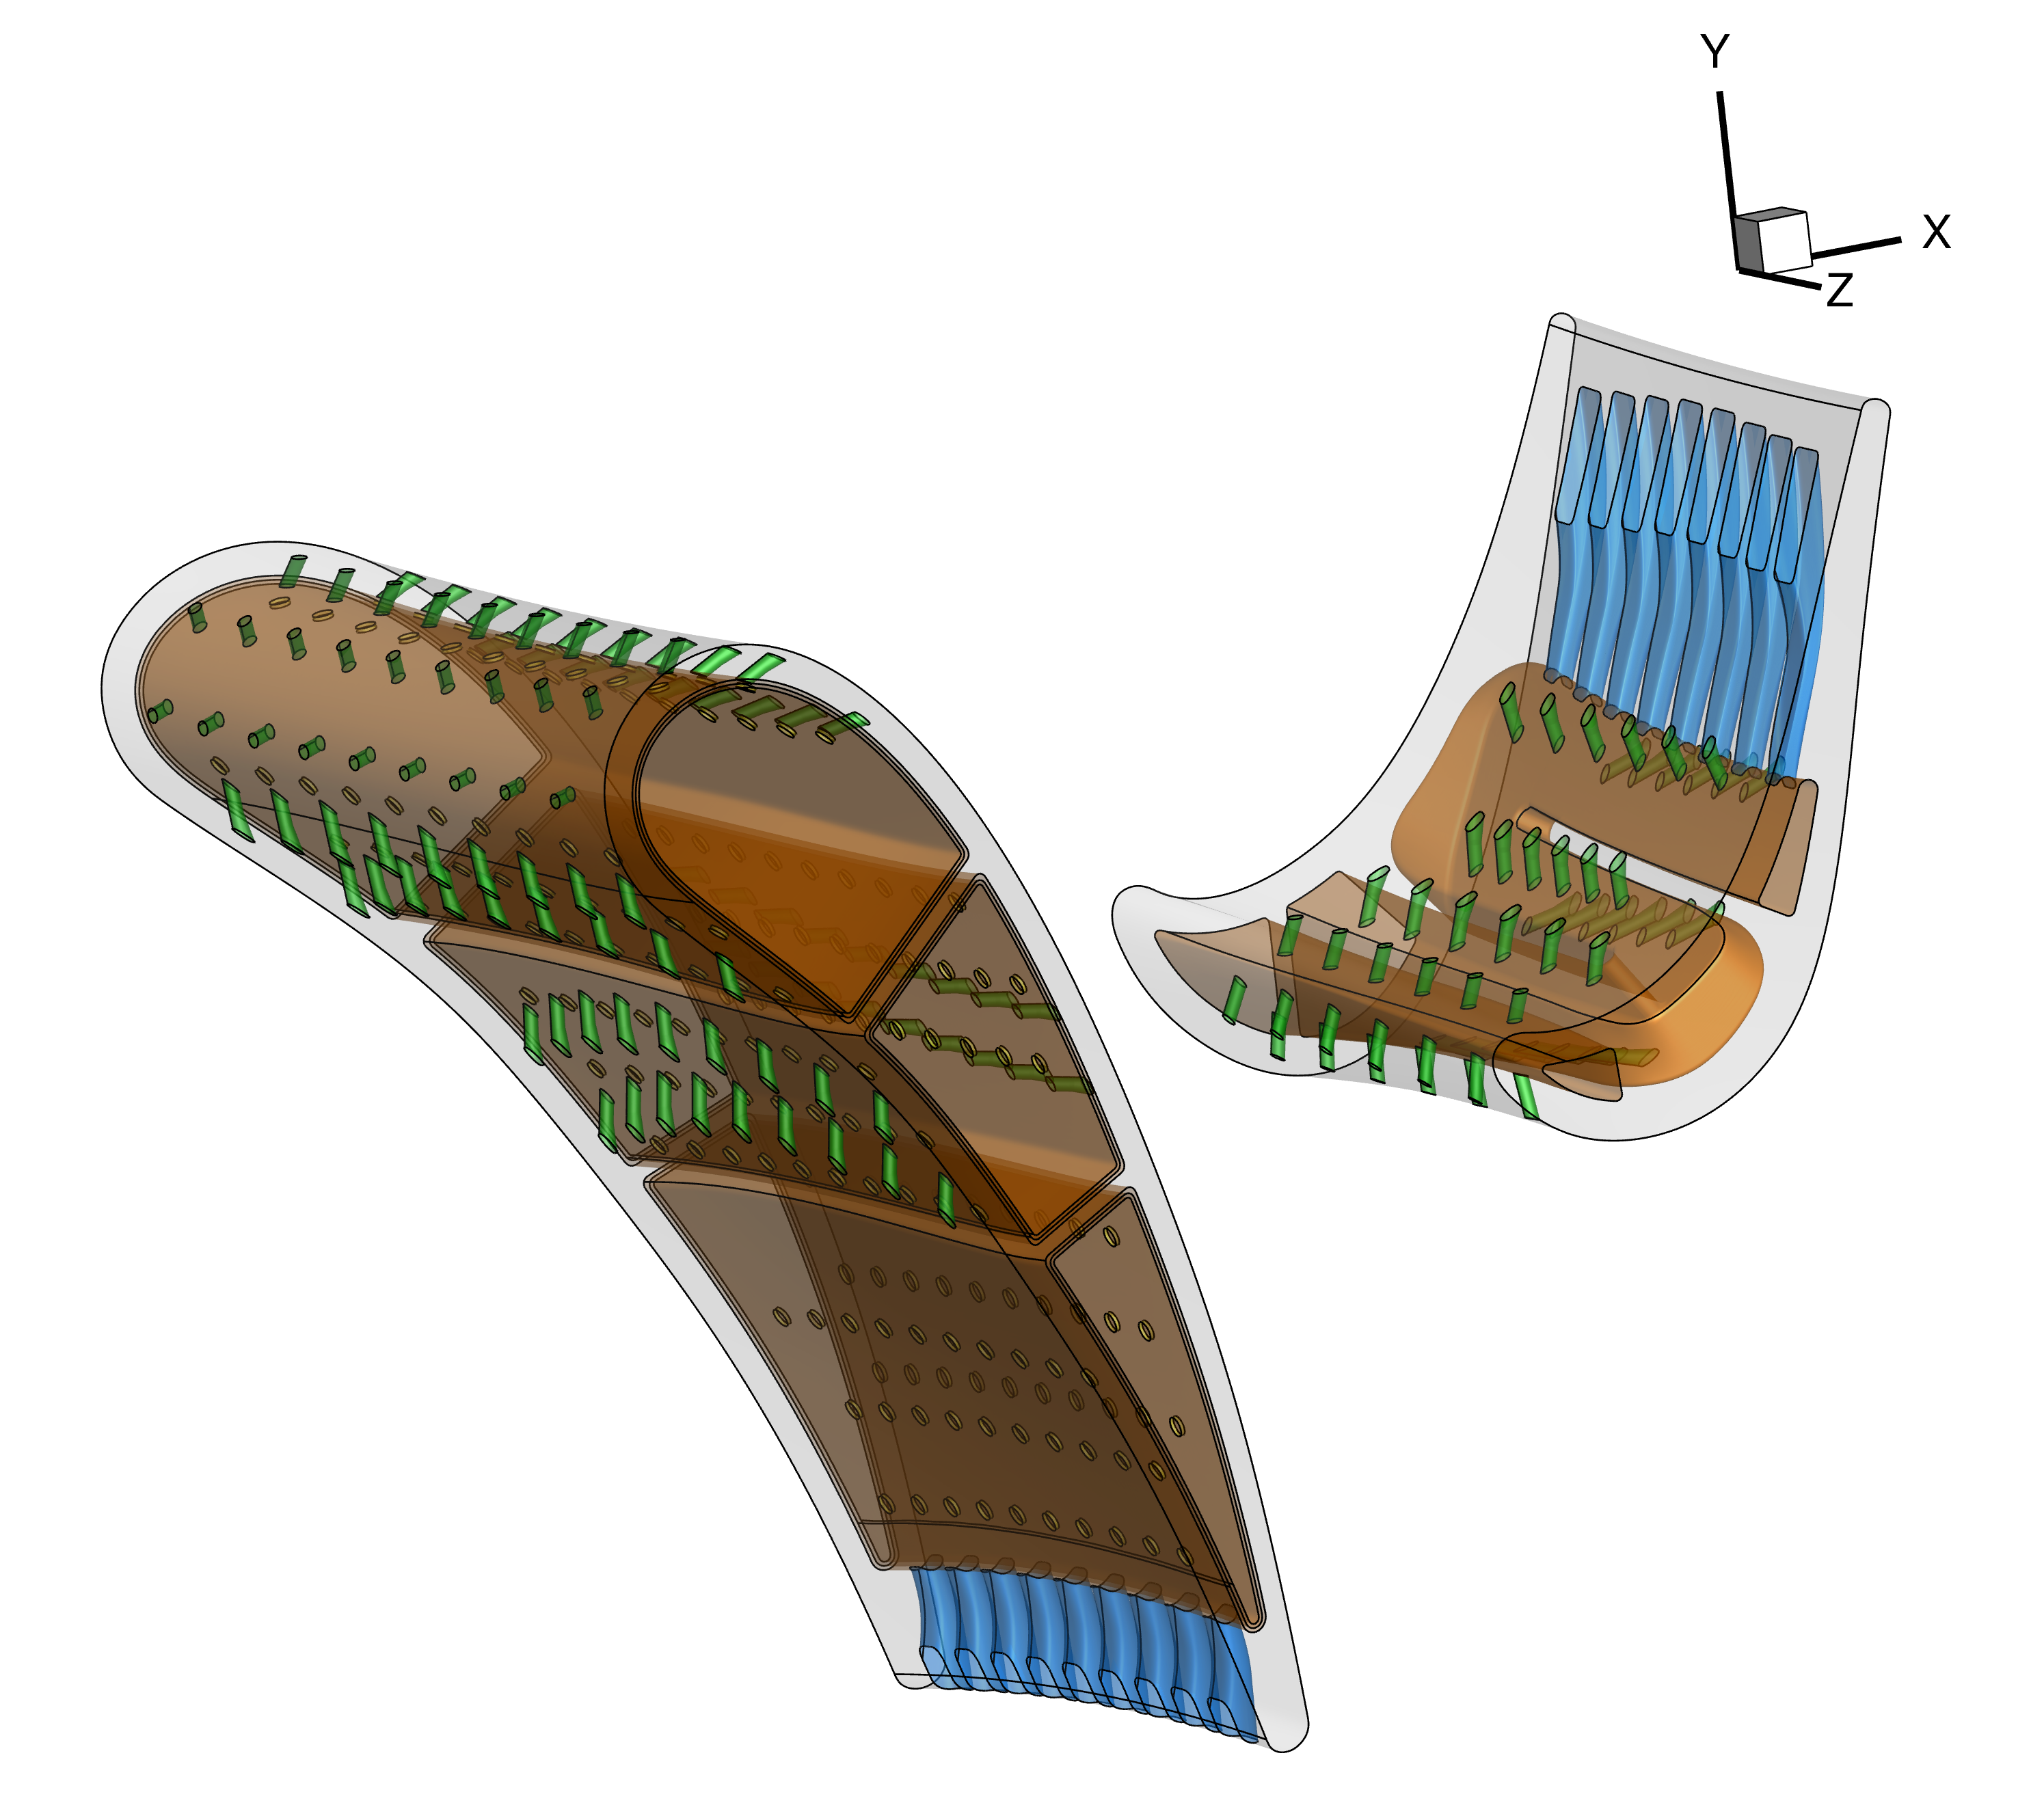
\includegraphics[width=\textwidth]{../../tec/complete/60.png}
		\end{figure}
	\end{minipage}
	\vfill
\end{frame}

\begin{frame}
	\frametitle{Geometrien / Überblick}
	\vspace{-1.5cm}\hspace{-0.5cm}
	\begin{minipage}[t]{0.38\textwidth}
		\begin{itemize}
			\item[\ding{108}] Kühlkanäle
			\item[\ding{40}] Filmkühlung
			\item[\ding{109}] Prallkühlung
			\item[\ding{109}] Ausblasungsschlitze
			\item[\ding{109}] Pin-fins
		\end{itemize}
	\end{minipage}
	\begin{minipage}{0.6\textwidth}
		\begin{figure}[H]
			\centering
			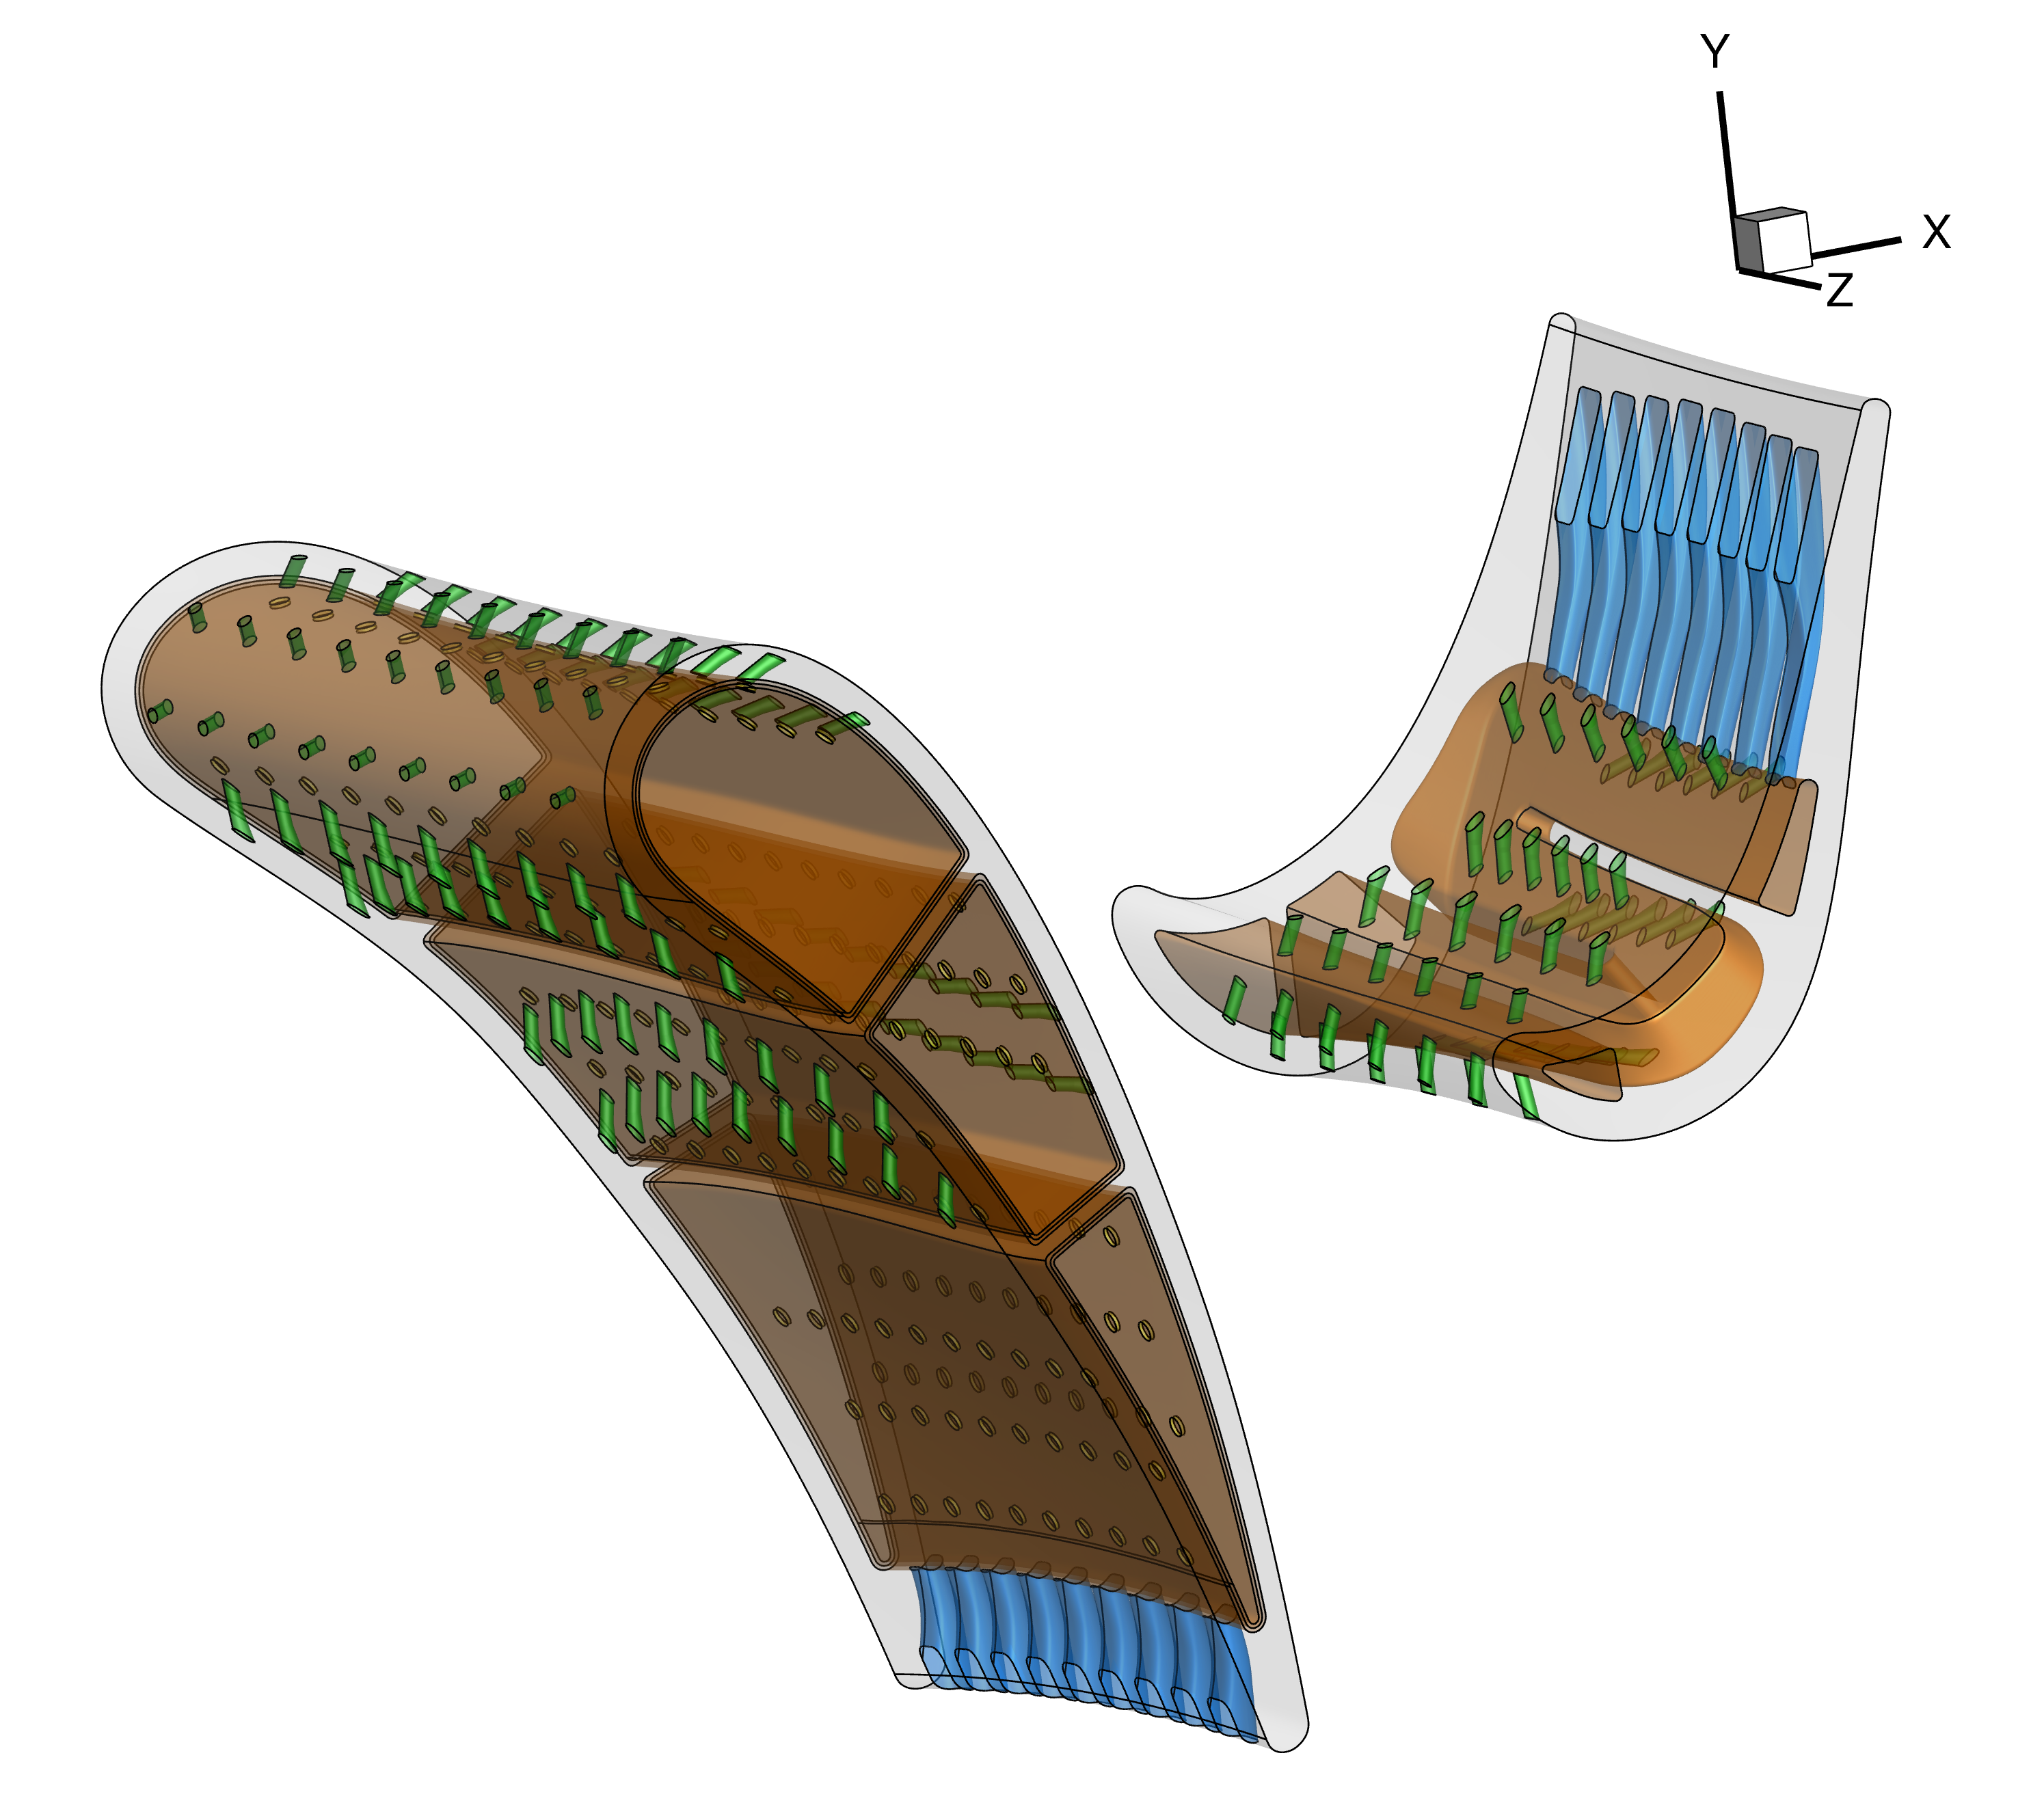
\includegraphics[width=\textwidth]{../../tec/complete/60.png}
		\end{figure}
	\end{minipage}
	\vfill
\end{frame}

\begin{frame}
	\frametitle{Geometrien / Filmkühlung}
	\vspace{-0.5cm}

	\centering
	\begin{minipage}[t]{\textwidth}
		\begin{figure}[H]
			\centering
			\begin{subfigure}{.75\textwidth}
				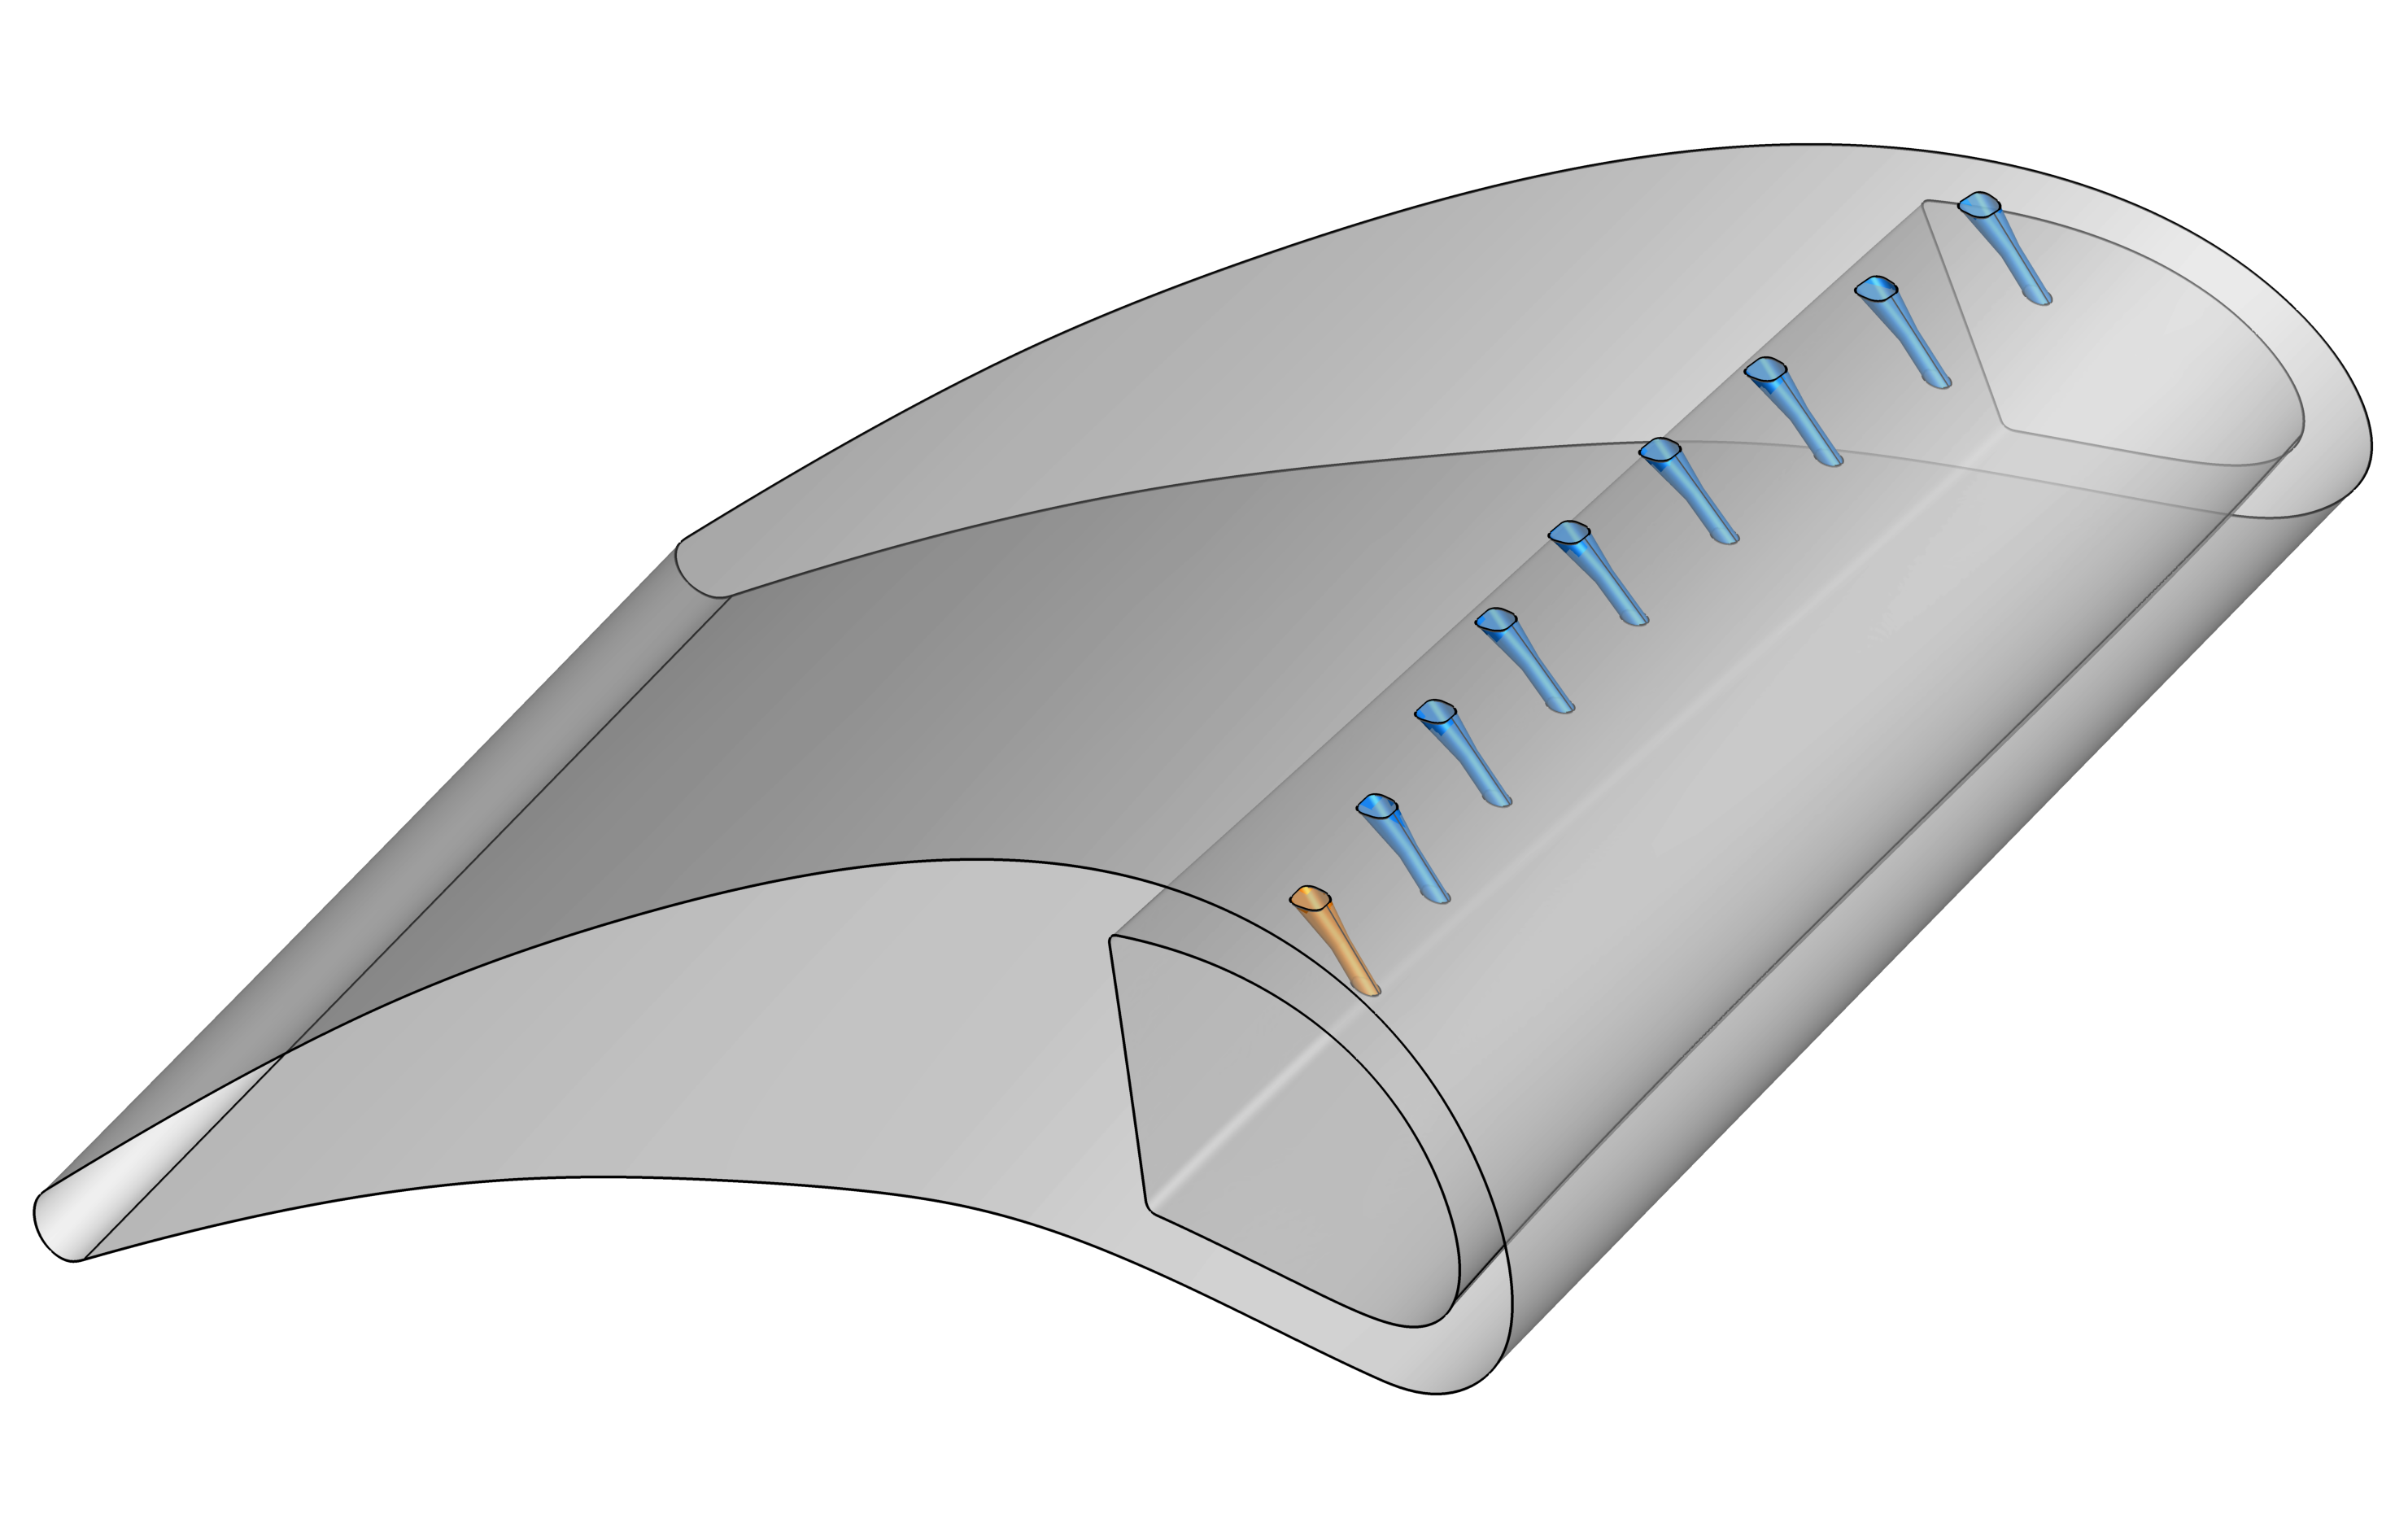
\includegraphics[width=\textwidth]{../../tec/holes/22edit.png}
			\end{subfigure}
		\end{figure}
	\end{minipage}
	\vfill
\end{frame}

\begin{frame}
	\frametitle{Geometrien / Filmkühlung}
	\vspace{-1.5cm}
	\centering
	\begin{minipage}[t]{\textwidth}
		\begin{figure}[H]
			\centering
			\begin{subfigure}{.15\textwidth}
				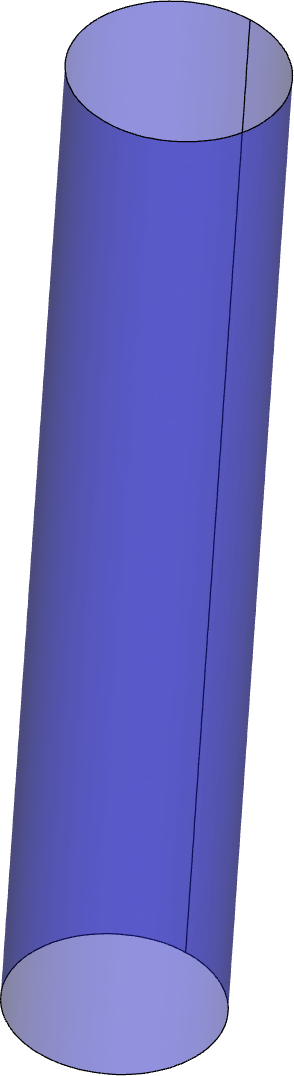
\includegraphics[width=0.6\textwidth]{../../tec/holes/16.png}
				\vspace{1cm}				
				\caption{Zylindrisch}
			\end{subfigure}
			\begin{subfigure}{.3\textwidth}
				\centering
				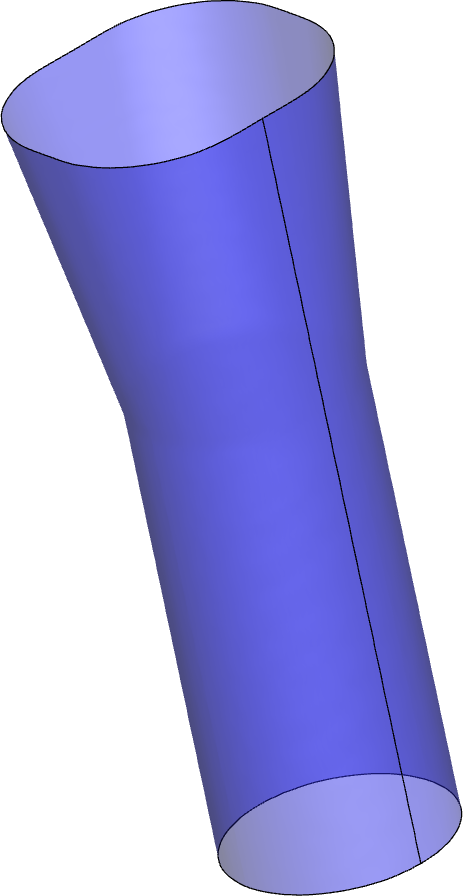
\includegraphics[width=.5\textwidth]{../../tec/holes/15.png}
				\vspace{1cm}
				\caption{Laid back fan-shaped}
			\end{subfigure}
			\begin{subfigure}{.5\textwidth}
				\includesvg[width=\textwidth]{../../python/fanshapedCurveDefinition}
				\caption{Begrenzende Kurven}
			\end{subfigure}
		\end{figure}
	\end{minipage}
	\vfill
\end{frame}

\begin{frame}
	\frametitle{Geometrien / Filmkühlung}
	\vspace{0cm}
	\centering
	\begin{minipage}[t]{.5\textwidth}
		\begin{figure}[H]
			\centering
			\begin{subfigure}{.49\textwidth}
				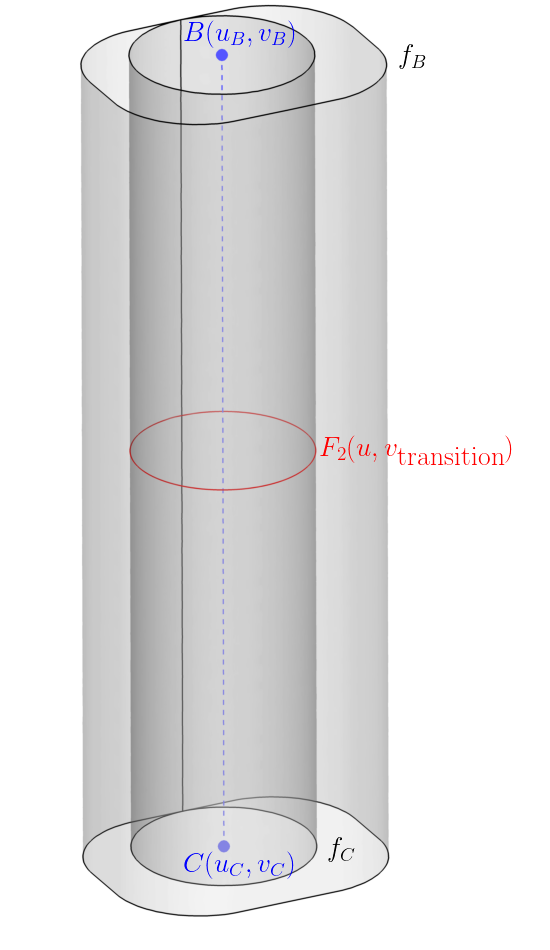
\includegraphics[width=\textwidth]{../../tec/holes/00edit.png}
			\end{subfigure}
			\begin{subfigure}{.49\textwidth}
				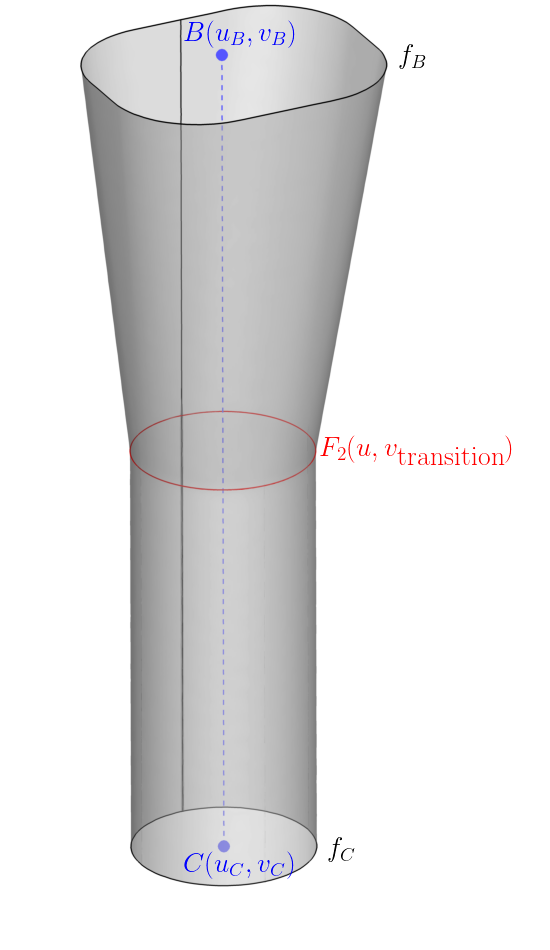
\includegraphics[width=\textwidth]{../../tec/holes/01edit.png}
			\end{subfigure}
		\end{figure}
	\end{minipage}
	\begin{minipage}[t]{.49\textwidth}
		\vspace{1cm}
		Links: Einbettung der 2D Kurven im 3D Raum entlang einer Strecke zwischen Schaufel $B$ und Kanal $C$.\\[1em]
		Rechts: Linearkombination der resultierenden Körper. $v_{\textrm{transition}}$ ist ein Eingabeparameter.
	\end{minipage}
	\vfill
\end{frame}

\begin{frame}
	\frametitle{Geometrien / Filmkühlung}
	\vspace{-0.5cm}
	\centering
	\begin{minipage}[t]{.4\textwidth}
		\begin{figure}[H]
			\centering
			\begin{subfigure}{\textwidth}
				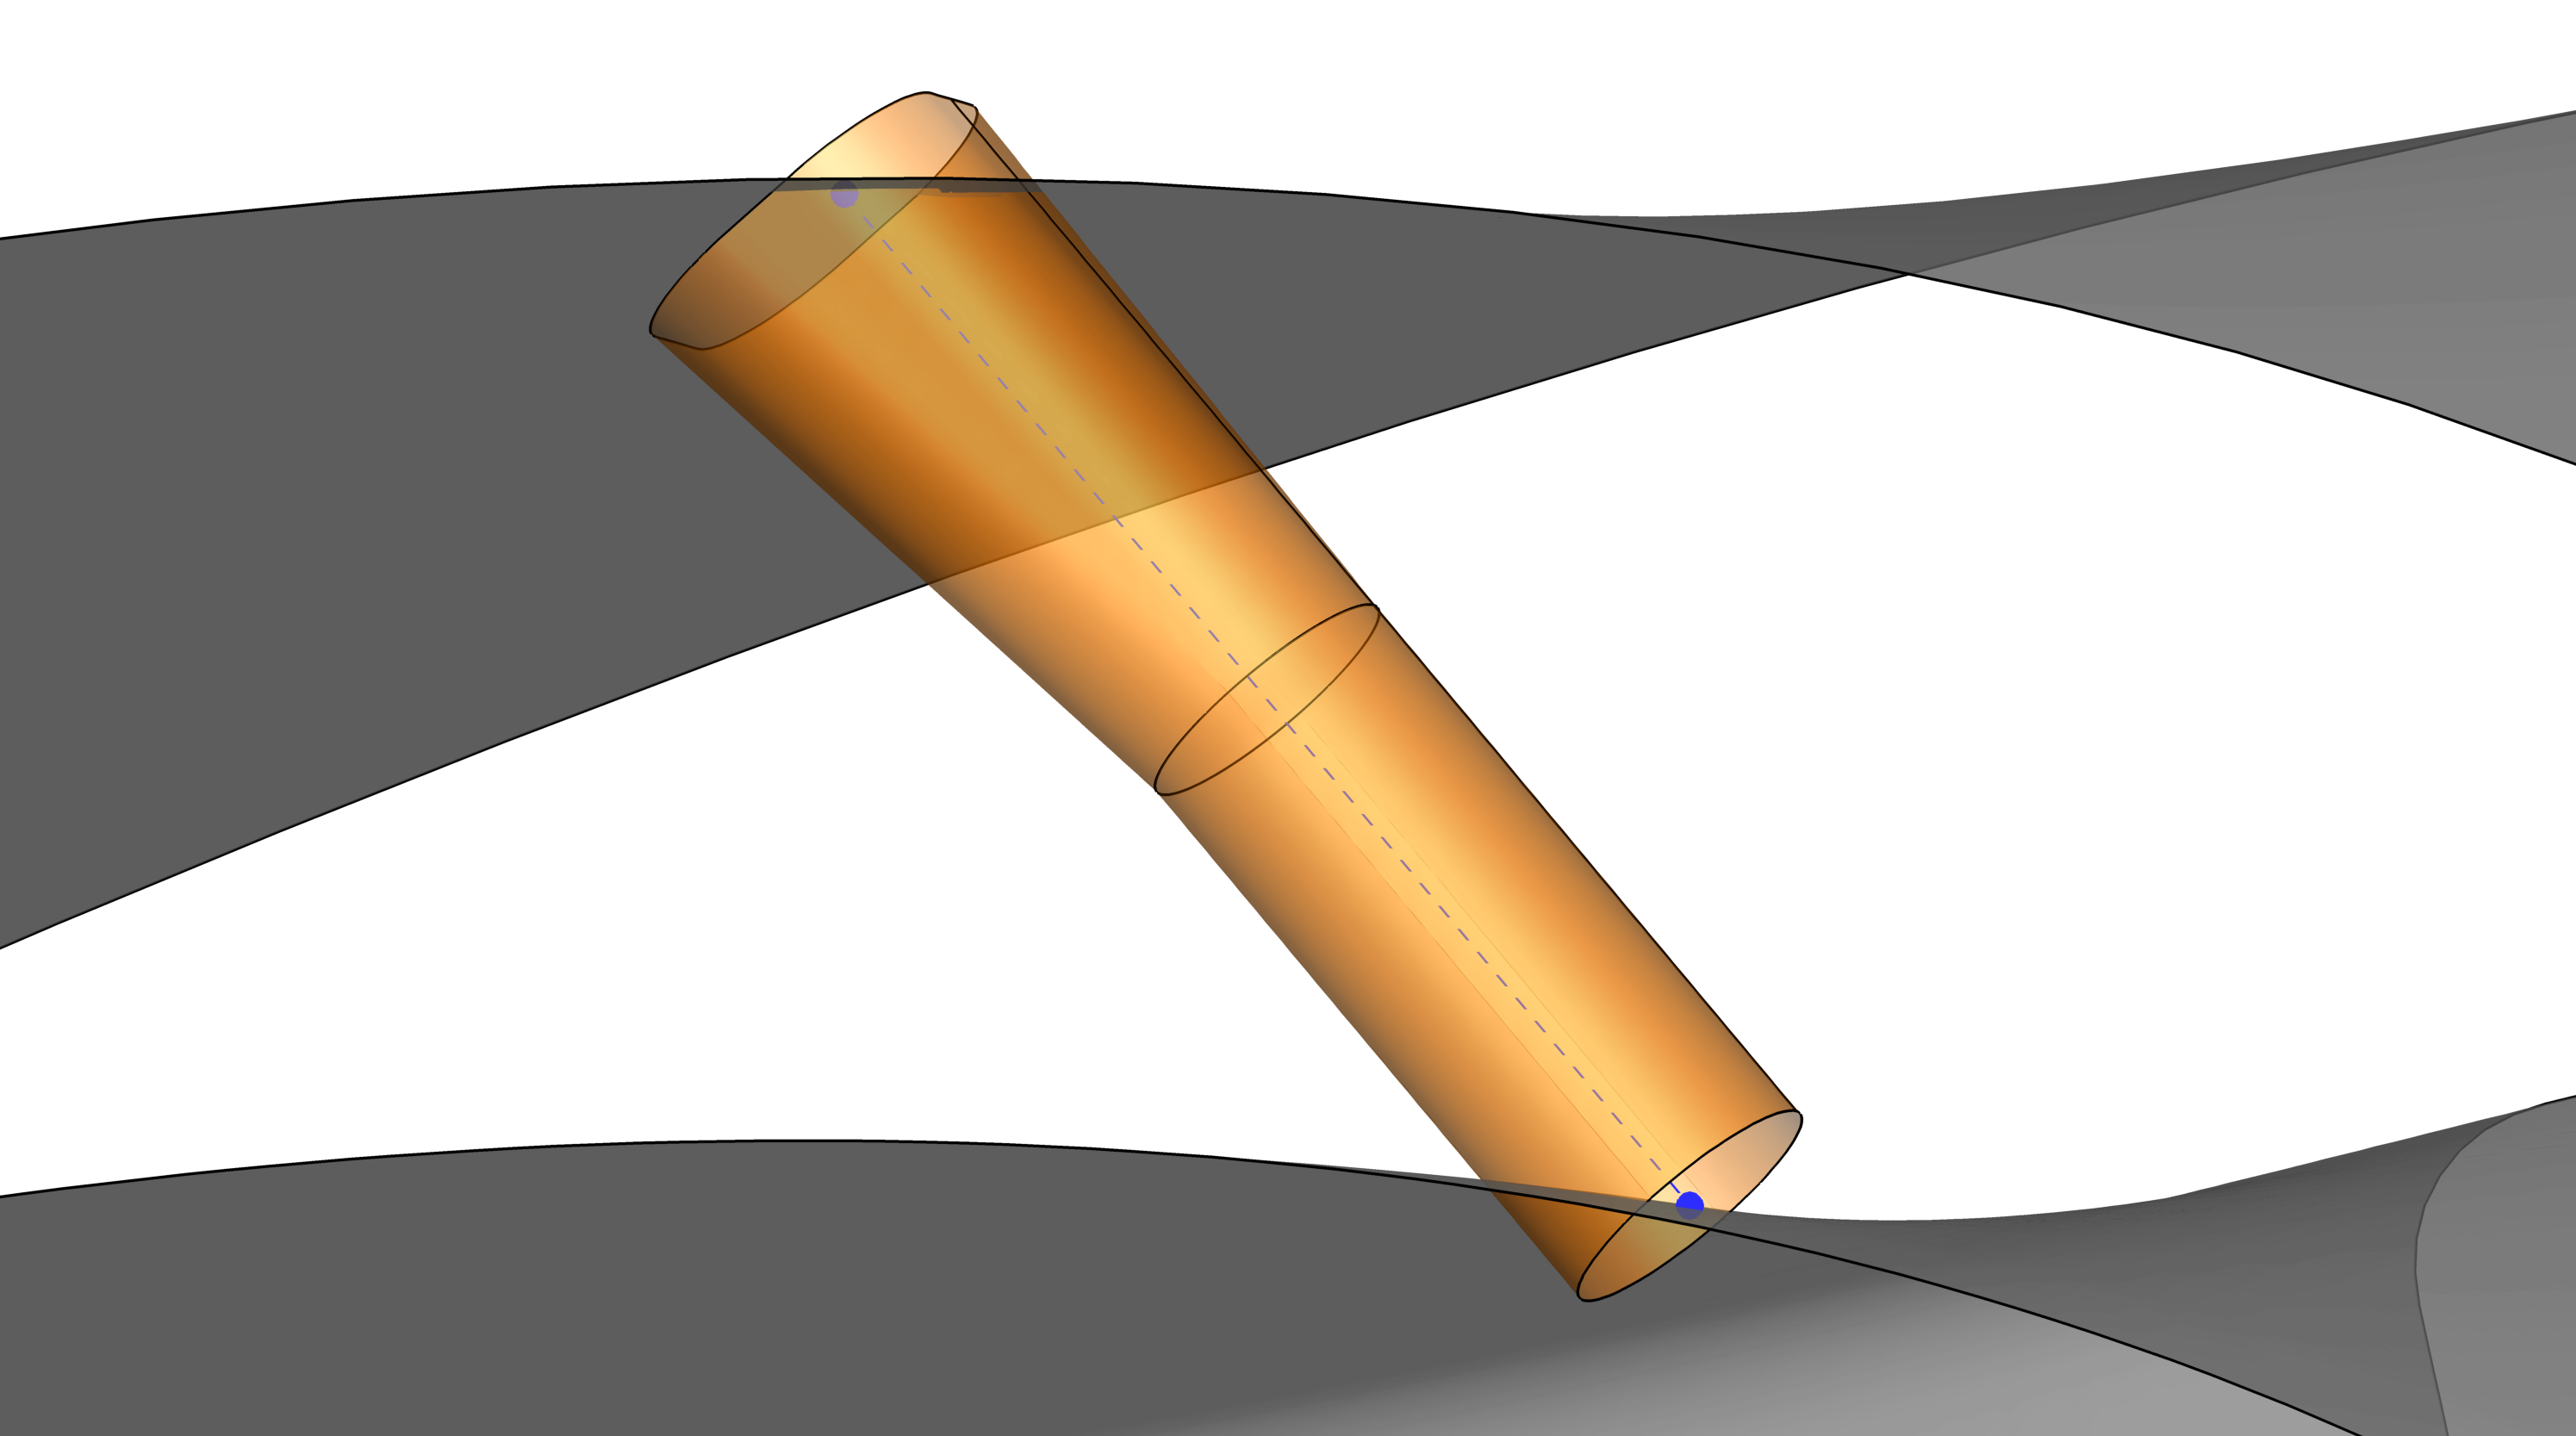
\includegraphics[width=\textwidth]{../../tec/holes/20edit.png}
			\end{subfigure}\\
			$\Downarrow$\\
			\begin{subfigure}{\textwidth}
				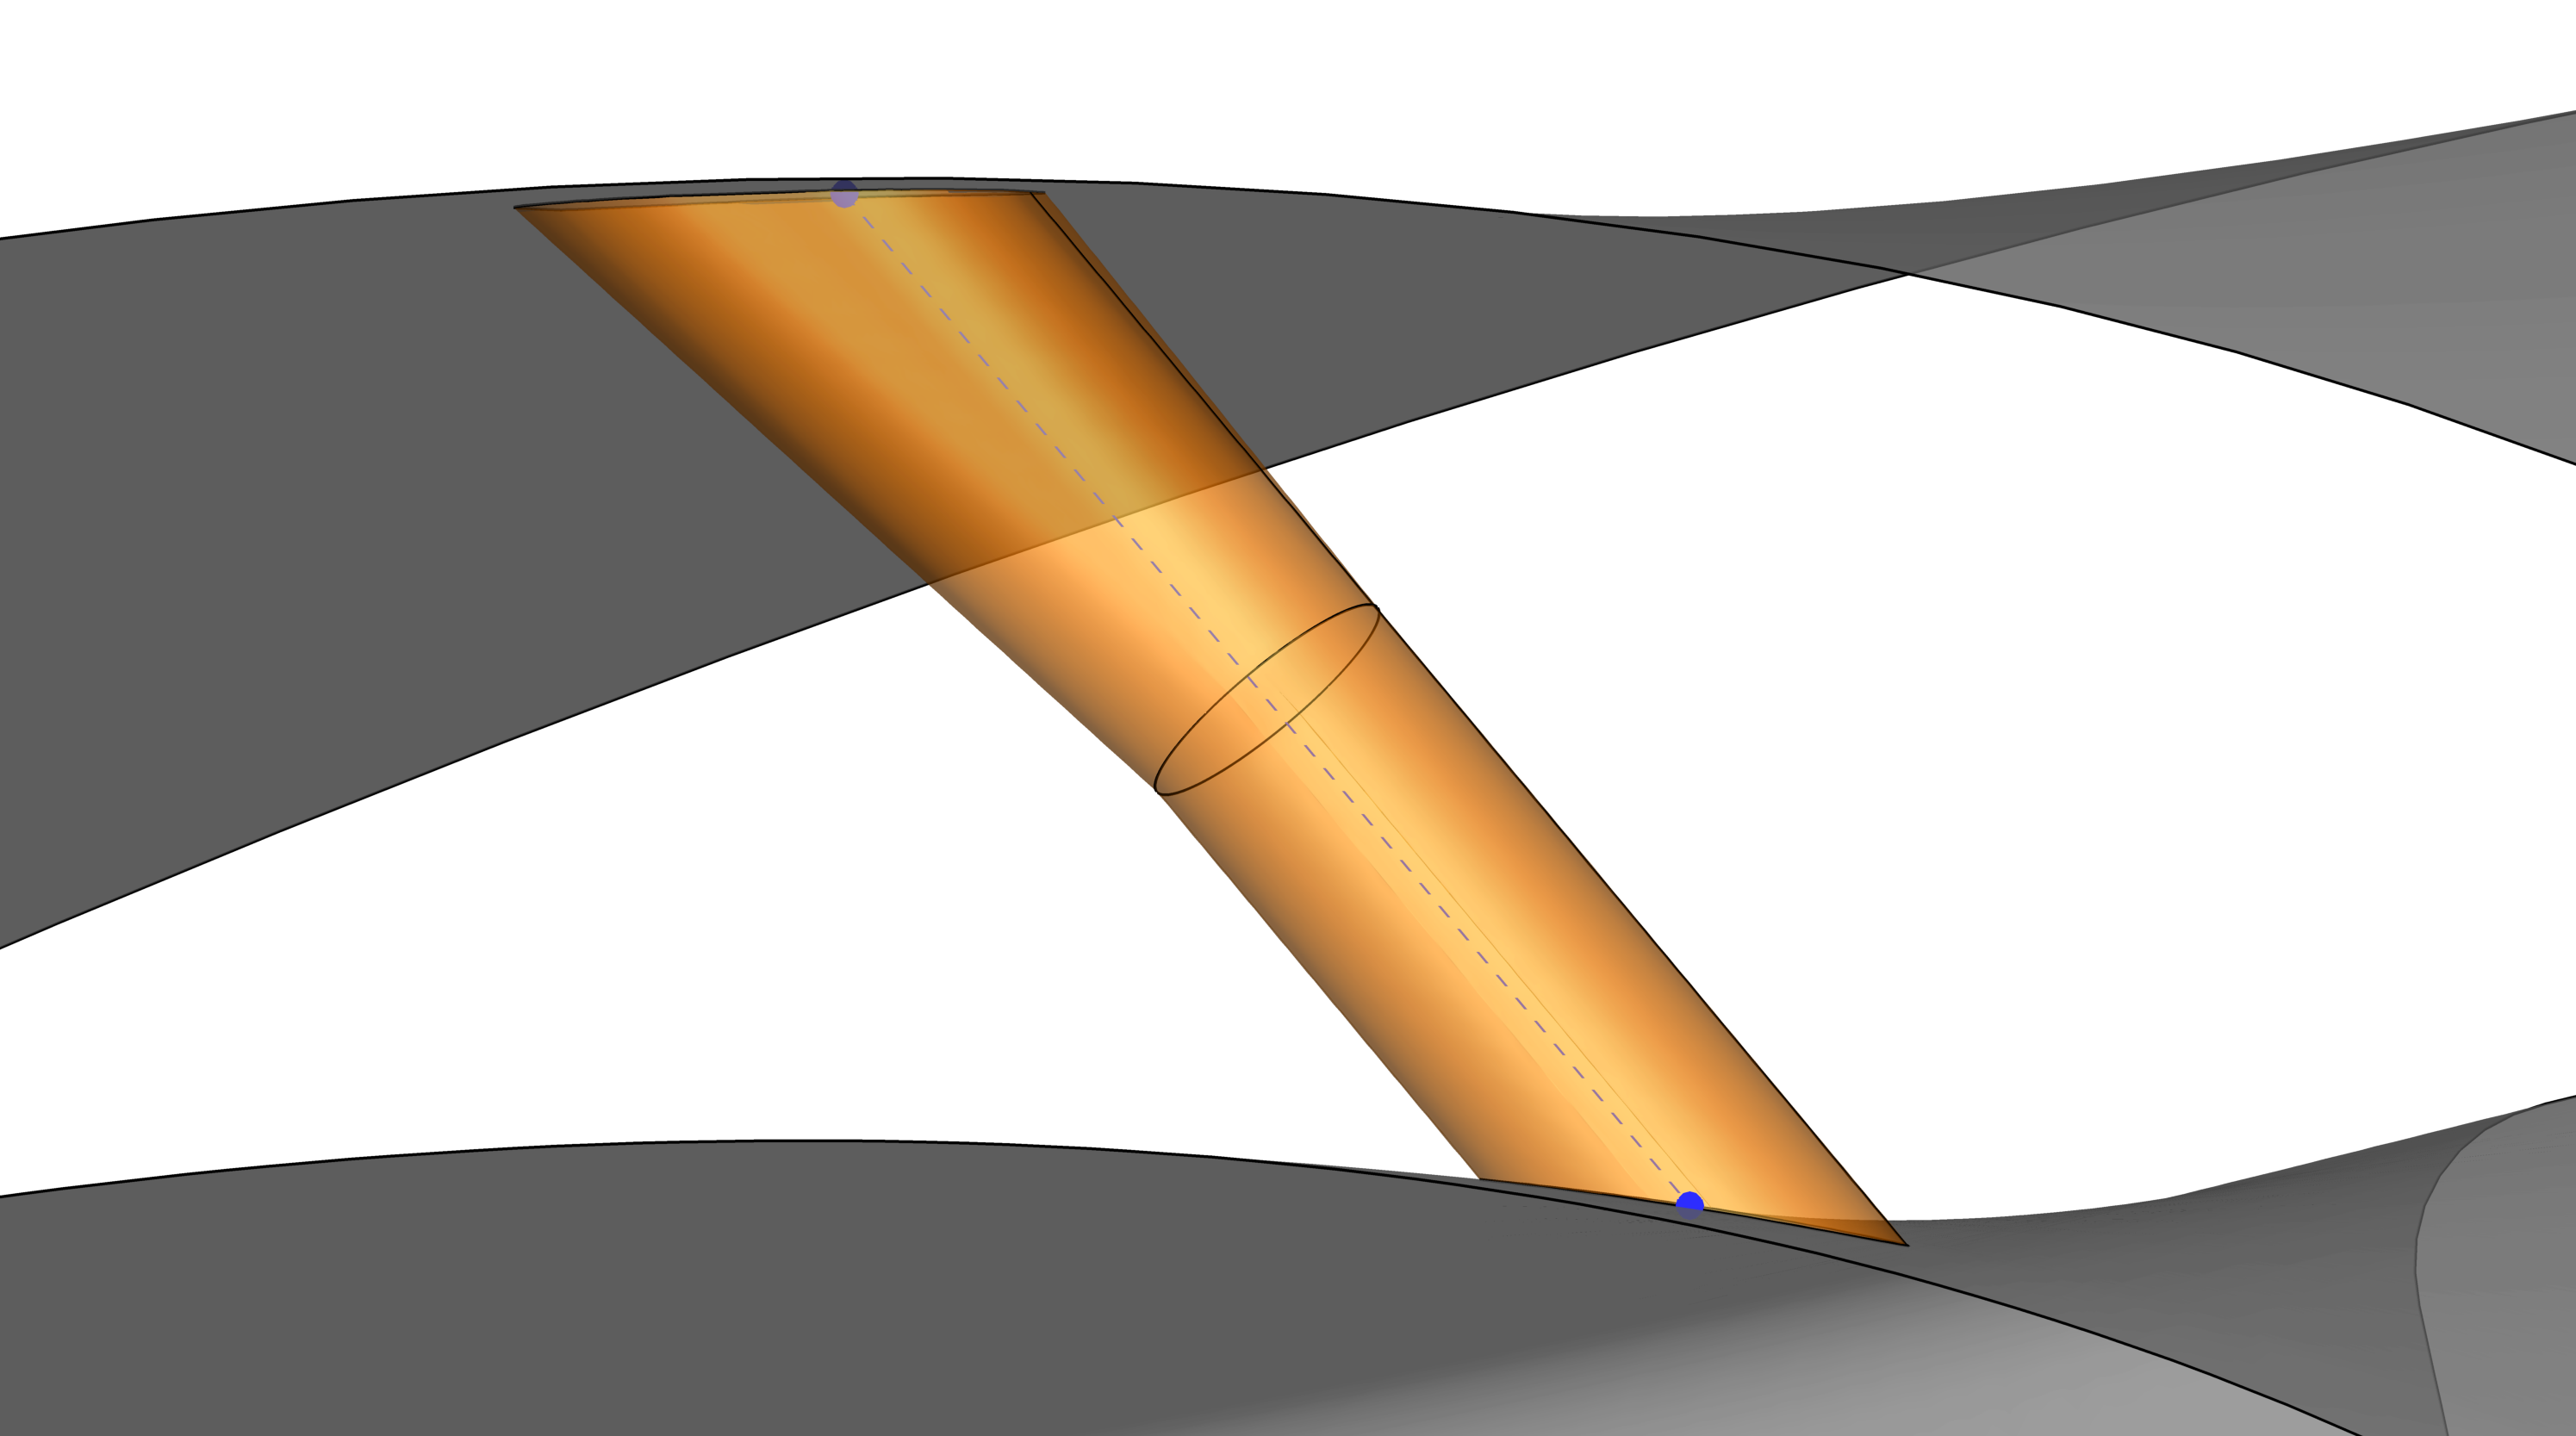
\includegraphics[width=\textwidth]{../../tec/holes/21edit.png}
			\end{subfigure}
		\end{figure}
	\end{minipage}
	\begin{minipage}[t]{.55\textwidth}
		\begin{figure}[H]
			\vspace{1cm}
			\centering
			Filmkühlungsbohrungen sind per Konstruktion Teilmengen von Halbgeraden (engl. \textbf{rays}).
			Wir nutzen \textbf{ray marching}, um die einzelnen Rays mit den umgebenden Flächen zu schneiden.
			\includesvg[width=\textwidth]{../../python/rayMarching}
		\end{figure}
	\end{minipage}
	\vfill
\end{frame}

\begin{frame}
	\frametitle{Geometrien / Filmkühlung}
	\vspace{-0.5cm}

	\centering
	\begin{minipage}[t]{\textwidth}
		\begin{figure}[H]
			\centering
			\begin{subfigure}{.75\textwidth}
				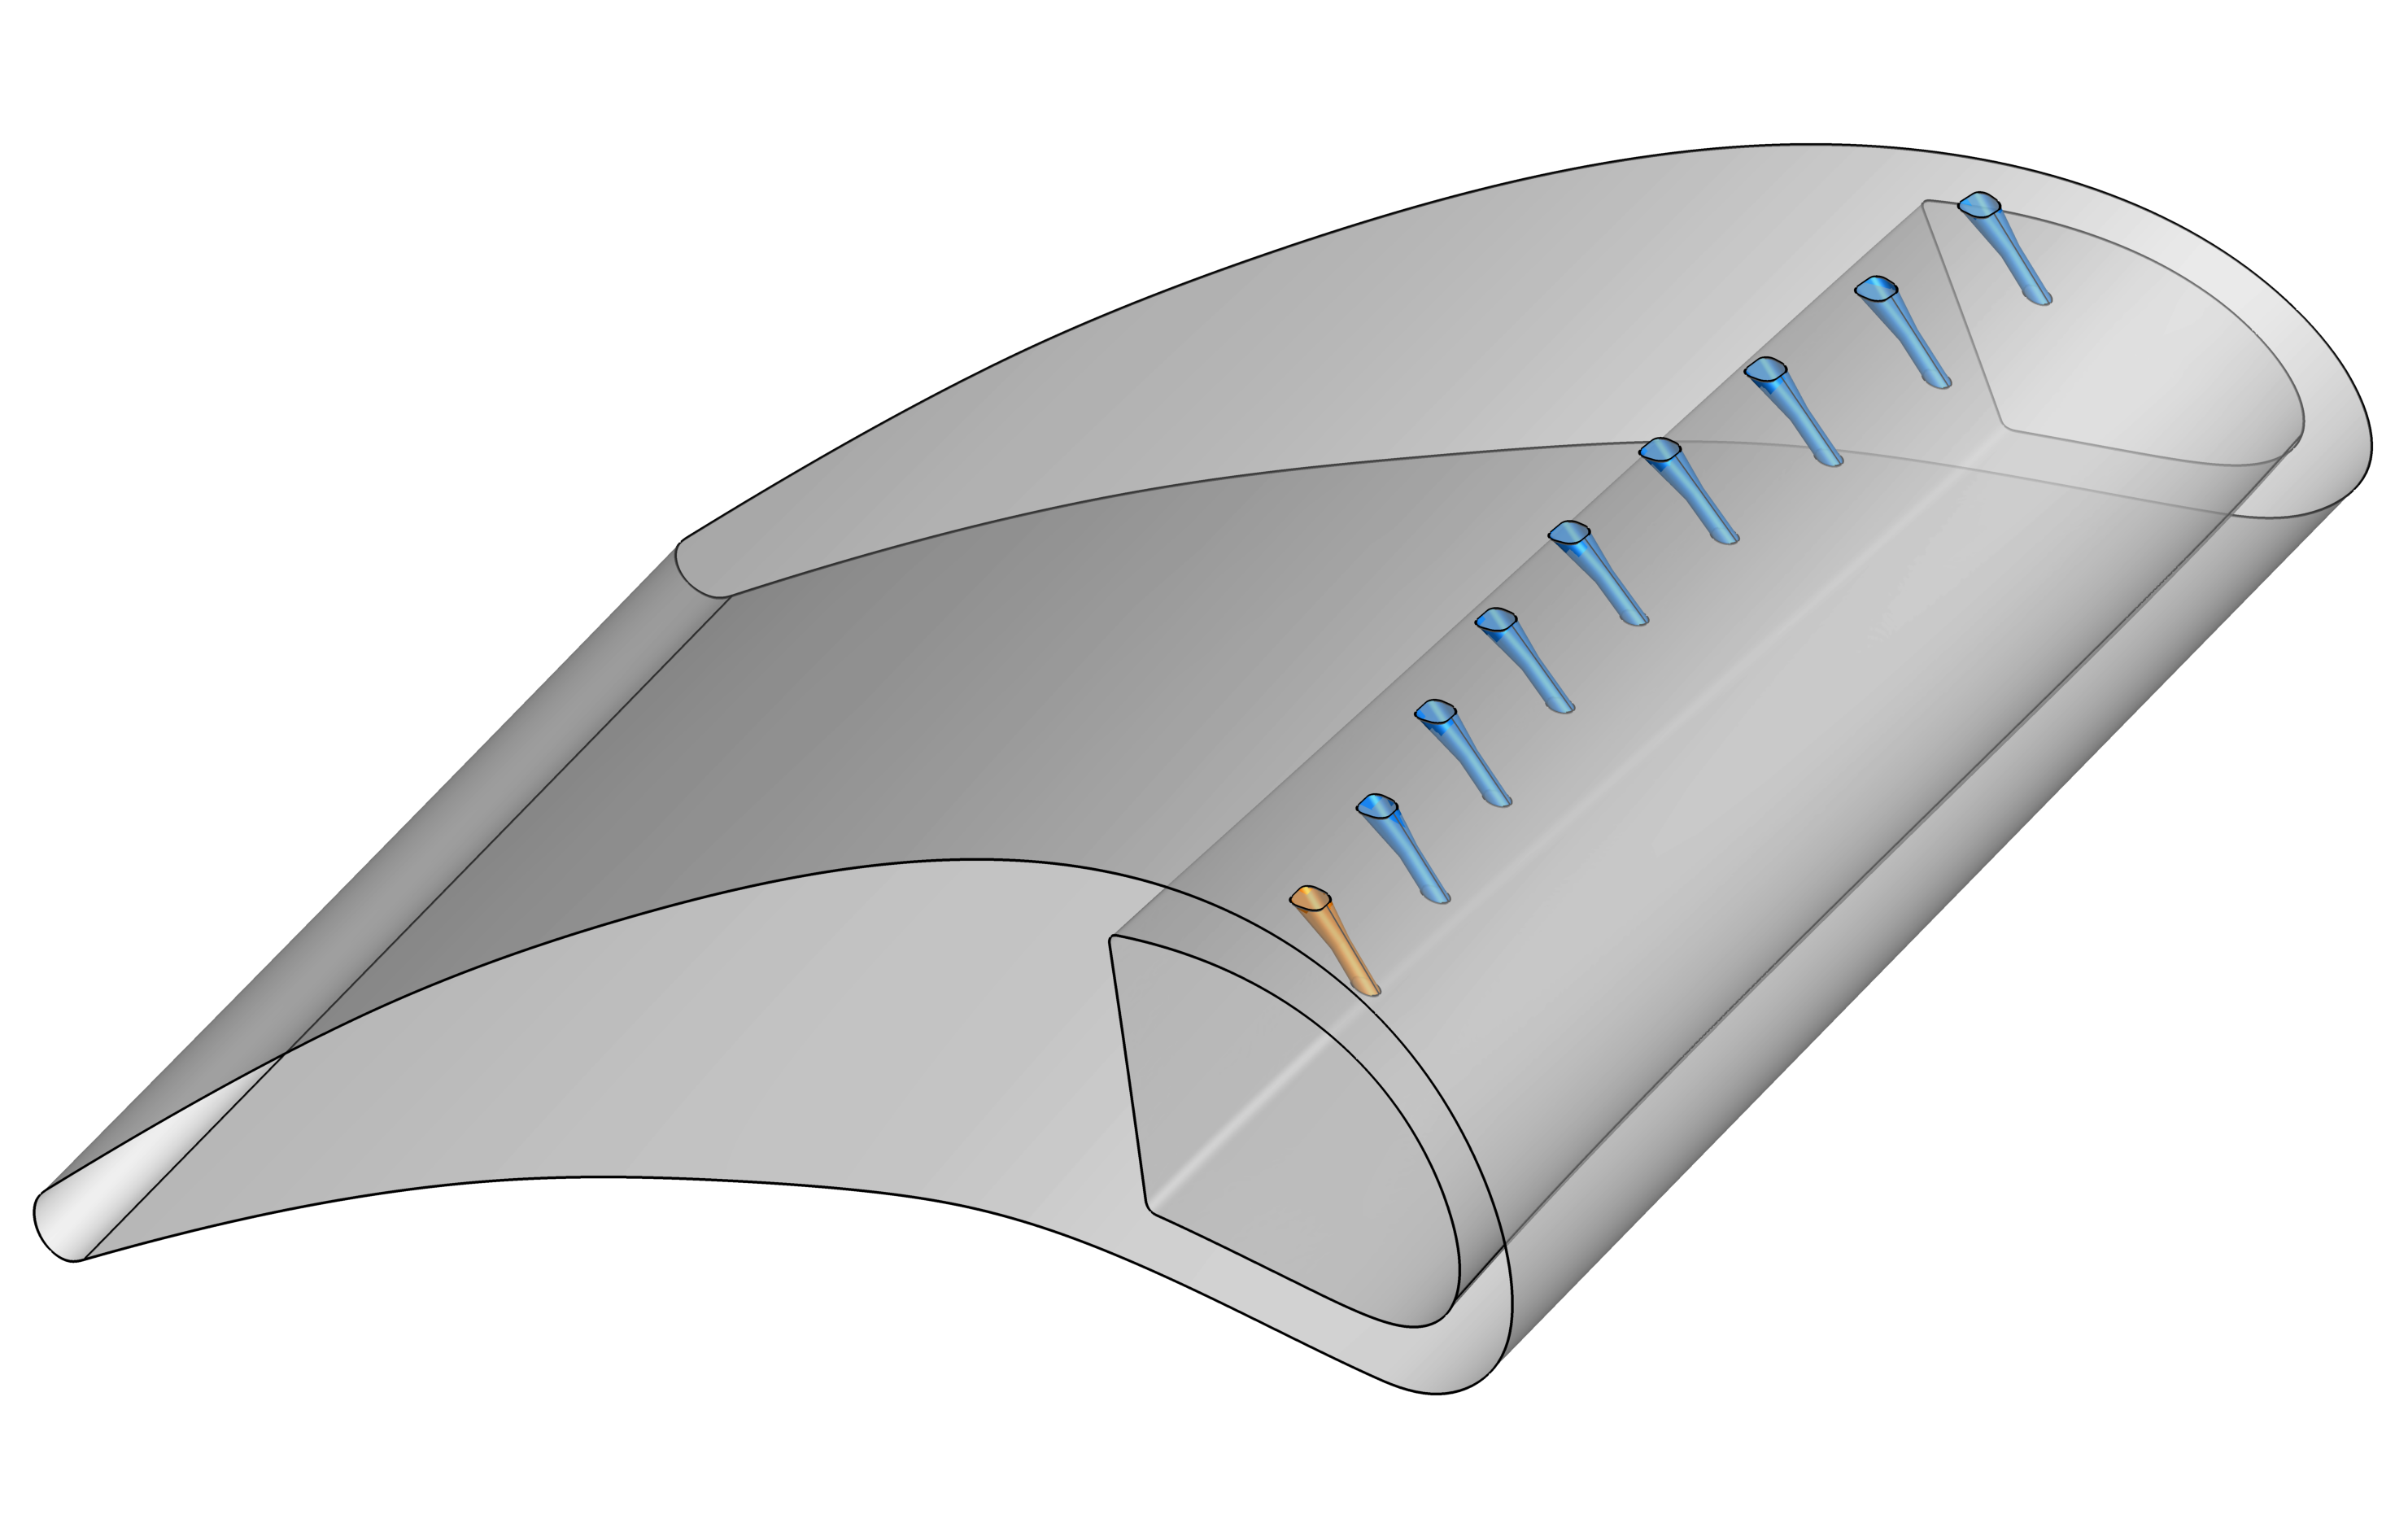
\includegraphics[width=\textwidth]{../../tec/holes/22edit.png}
			\end{subfigure}
		\end{figure}
	\end{minipage}
	\vfill
\end{frame}

\begin{frame}
	\frametitle{Geometrien / Überblick}
	\vspace{-1.5cm}\hspace{-0.5cm}
	\begin{minipage}[t]{0.38\textwidth}
		\begin{itemize}
			\item[\ding{108}] Kühlkanäle
			\item[\ding{108}] Filmkühlung
			\item[\ding{109}] Prallkühlung
			\item[\ding{109}] Ausblasungsschlitze
			\item[\ding{109}] Pin-fins
		\end{itemize}
	\end{minipage}
	\begin{minipage}{0.6\textwidth}
		\begin{figure}[H]
			\centering
			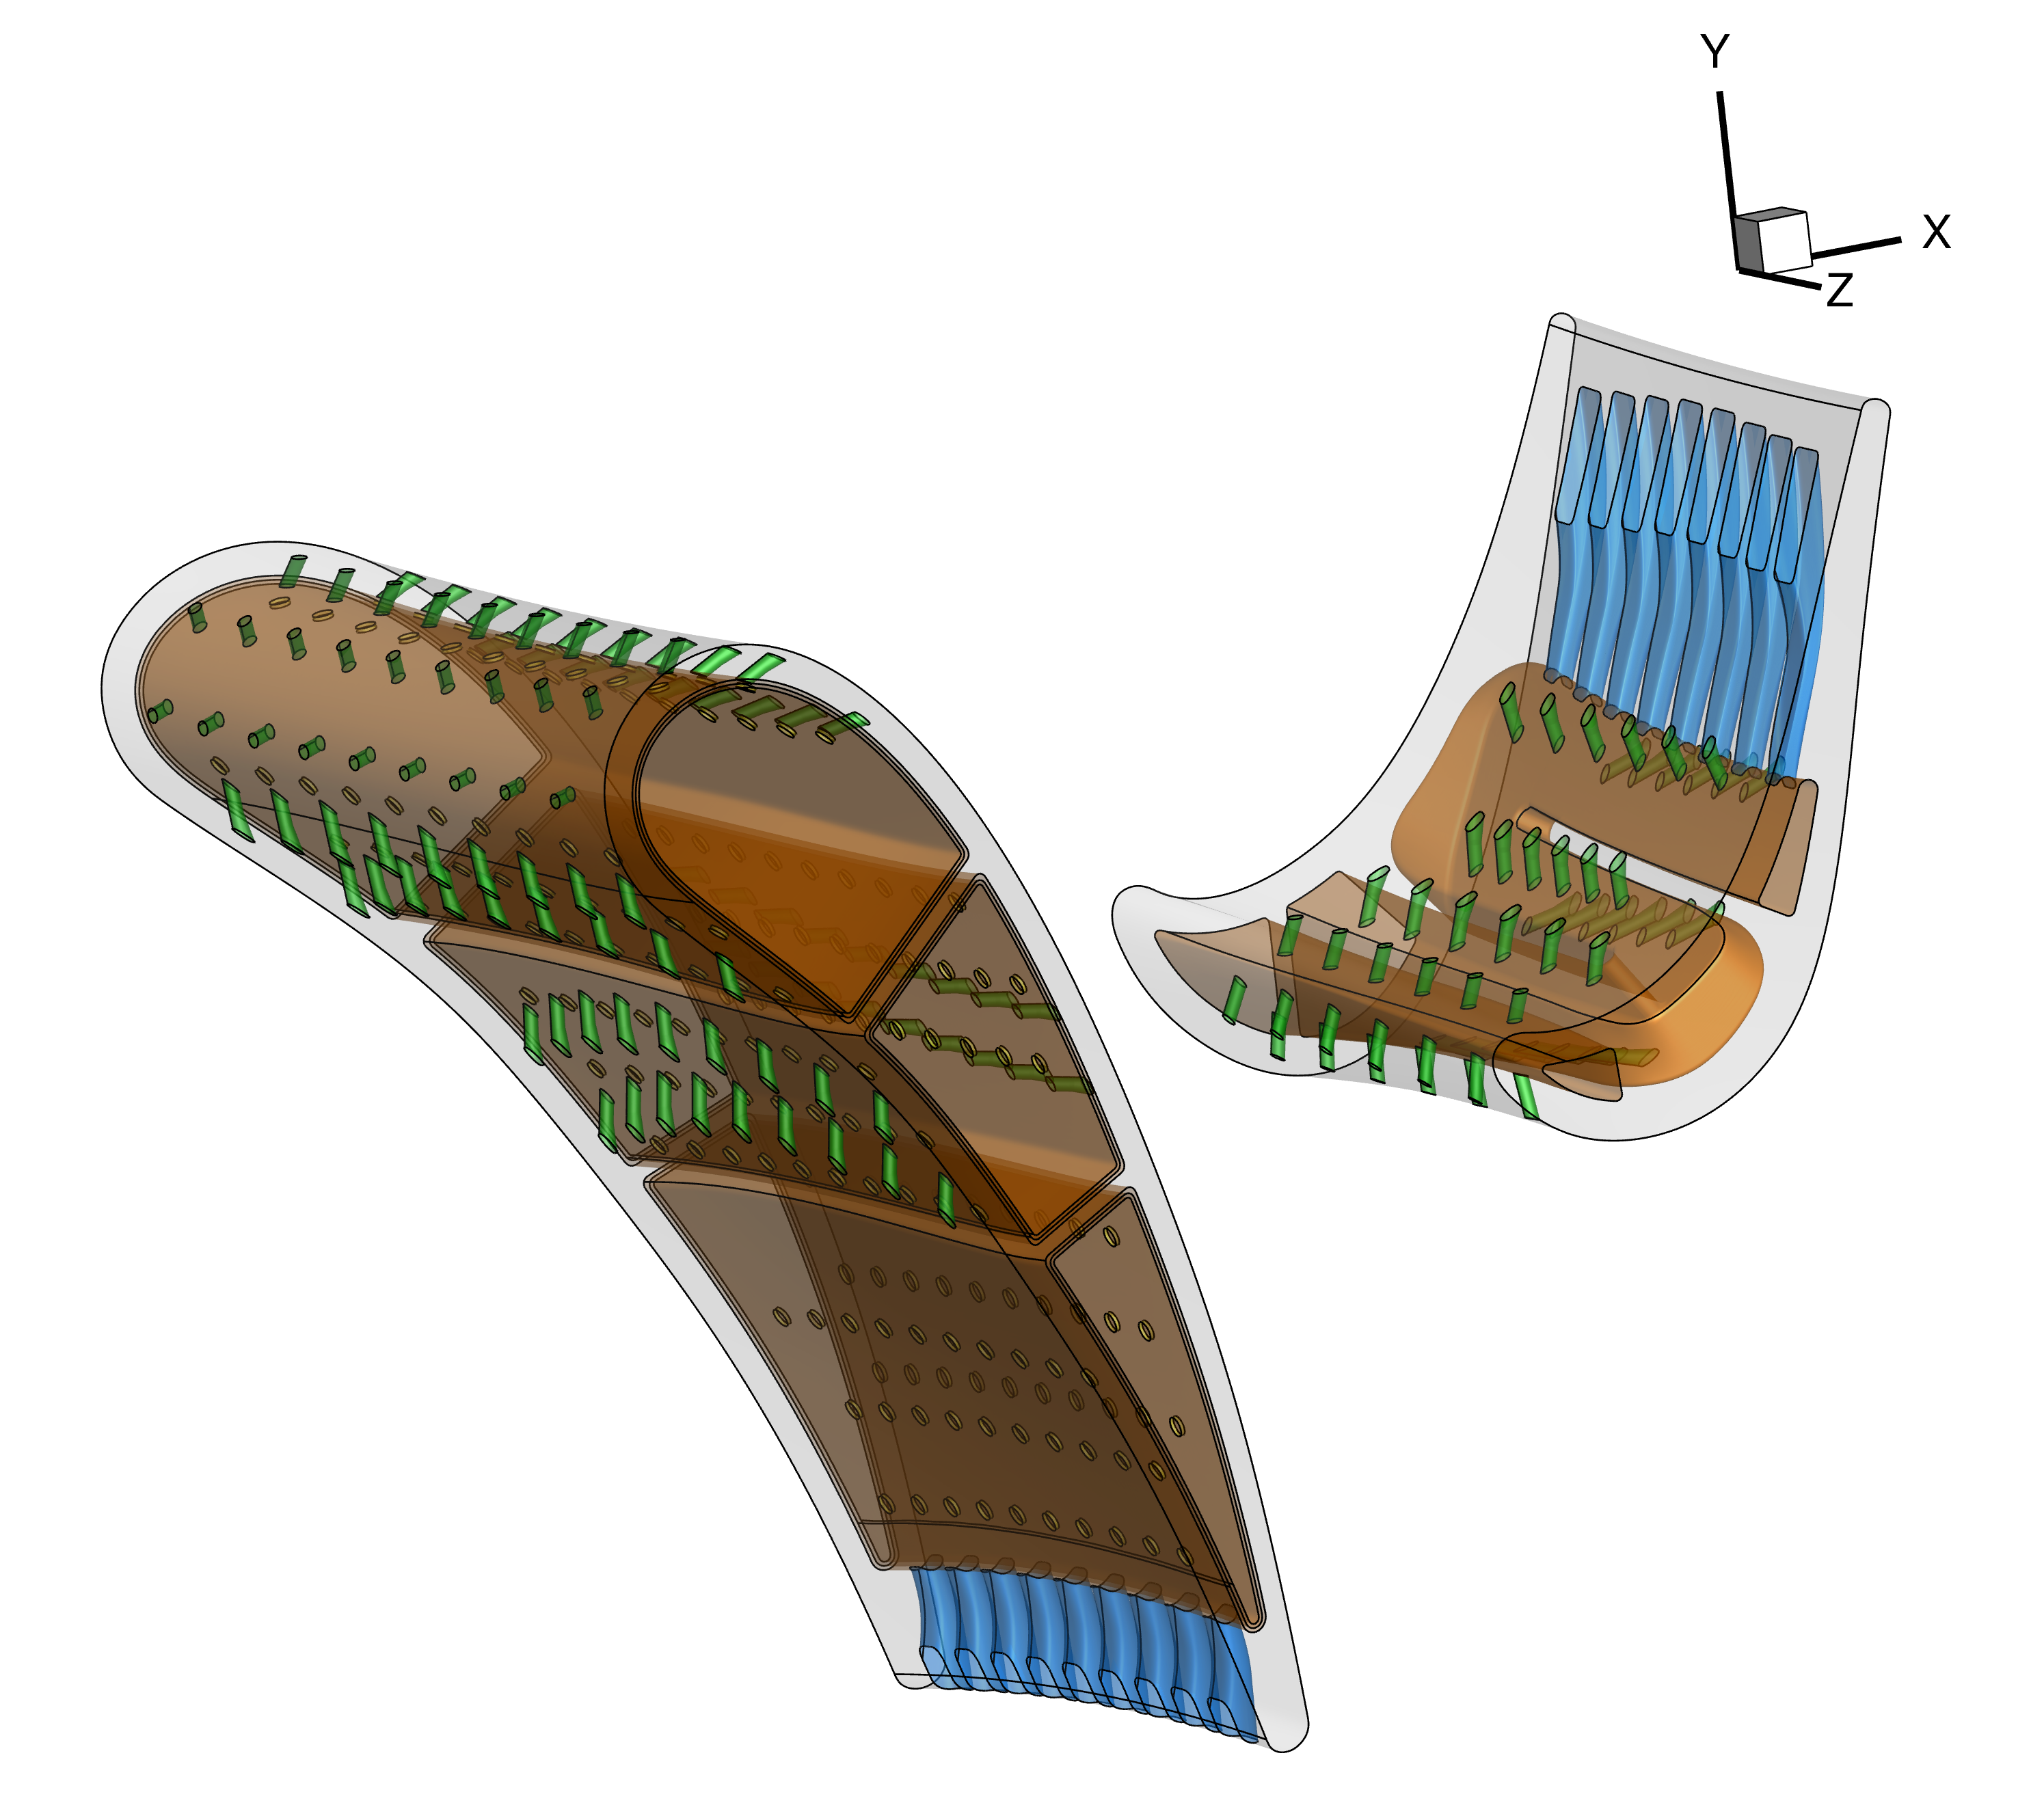
\includegraphics[width=\textwidth]{../../tec/complete/60.png}
		\end{figure}
	\end{minipage}
	\vfill
\end{frame}

\begin{frame}
	\frametitle{Geometrien / Überblick}
	\vspace{-1.5cm}\hspace{-0.5cm}
	\begin{minipage}[t]{0.38\textwidth}
		\begin{itemize}
			\item[\ding{108}] Kühlkanäle
			\item[\ding{108}] Filmkühlung
			\item[\ding{40}] Prallkühlung
			\item[\ding{109}] Ausblasungsschlitze
			\item[\ding{109}] Pin-fins
		\end{itemize}
	\end{minipage}
	\begin{minipage}{0.6\textwidth}
		\begin{figure}[H]
			\centering
			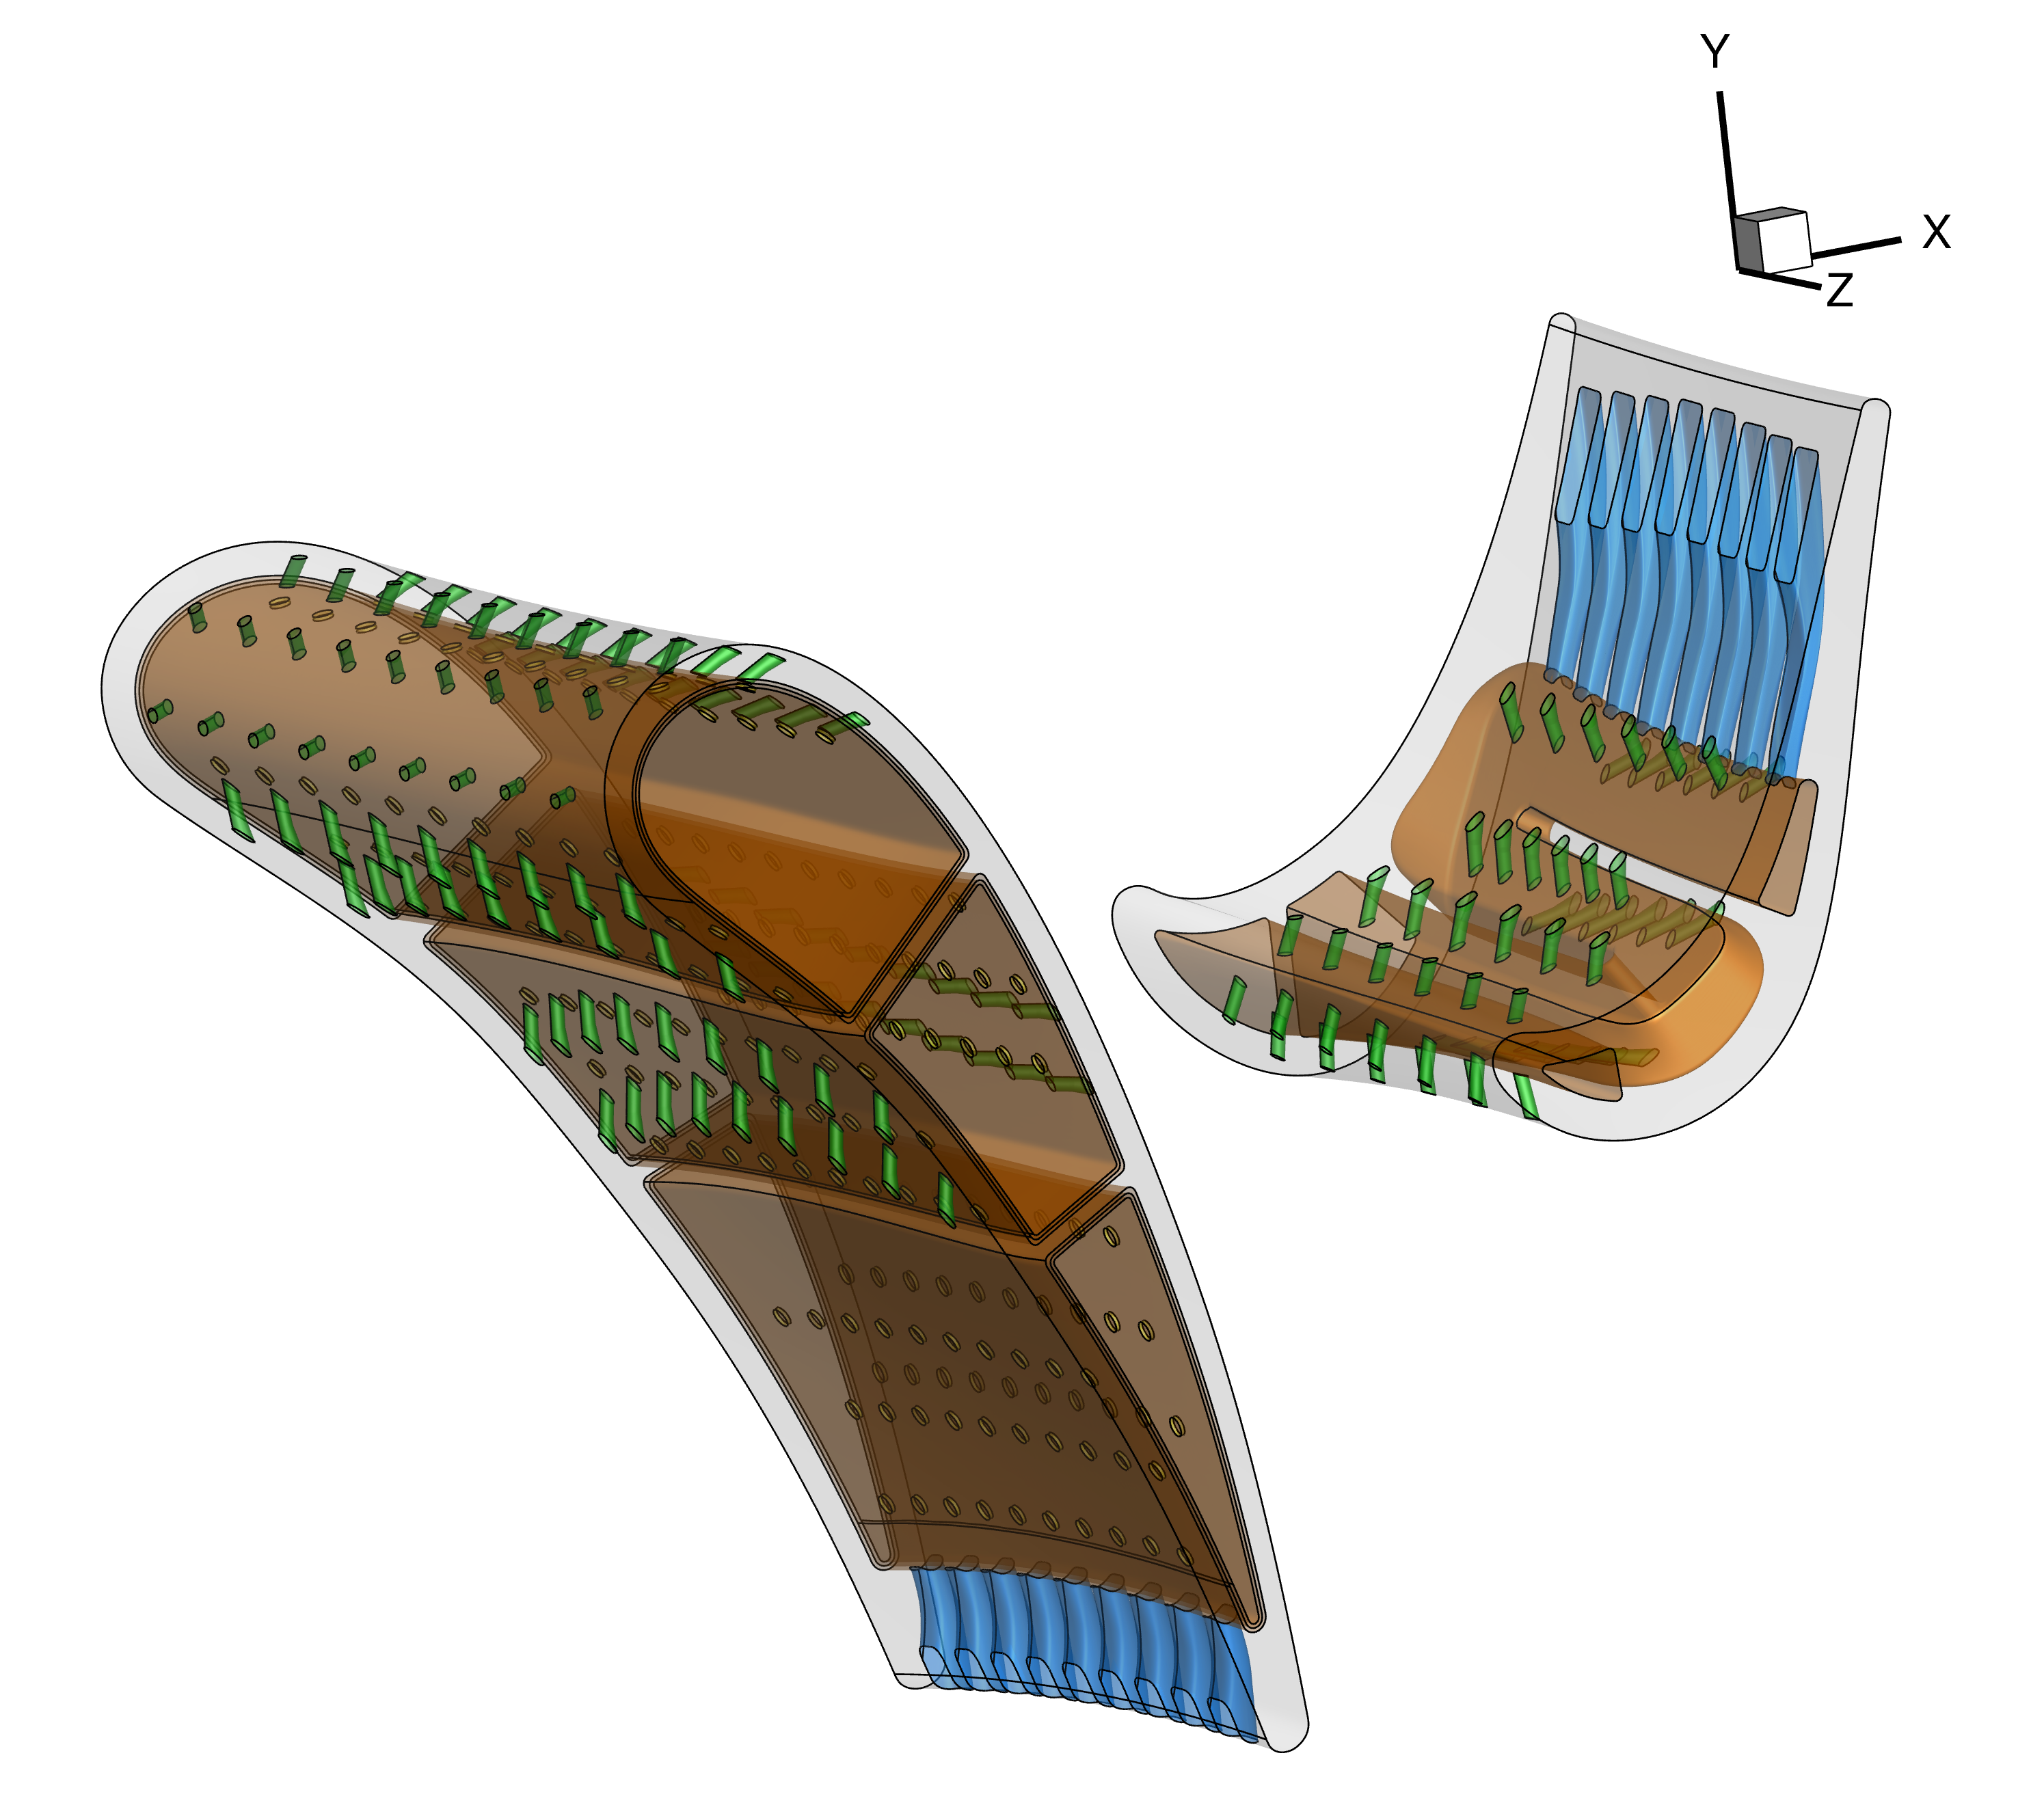
\includegraphics[width=\textwidth]{../../tec/complete/60.png}
		\end{figure}
	\end{minipage}
	\vfill
\end{frame}

\begin{frame}
	\frametitle{Geometrien / Prallkühlung}
	\vspace{-1.5cm}\hspace{-0.5cm}
	\begin{figure}[H]
		\centering
		\begin{subfigure}{.3\textwidth}
			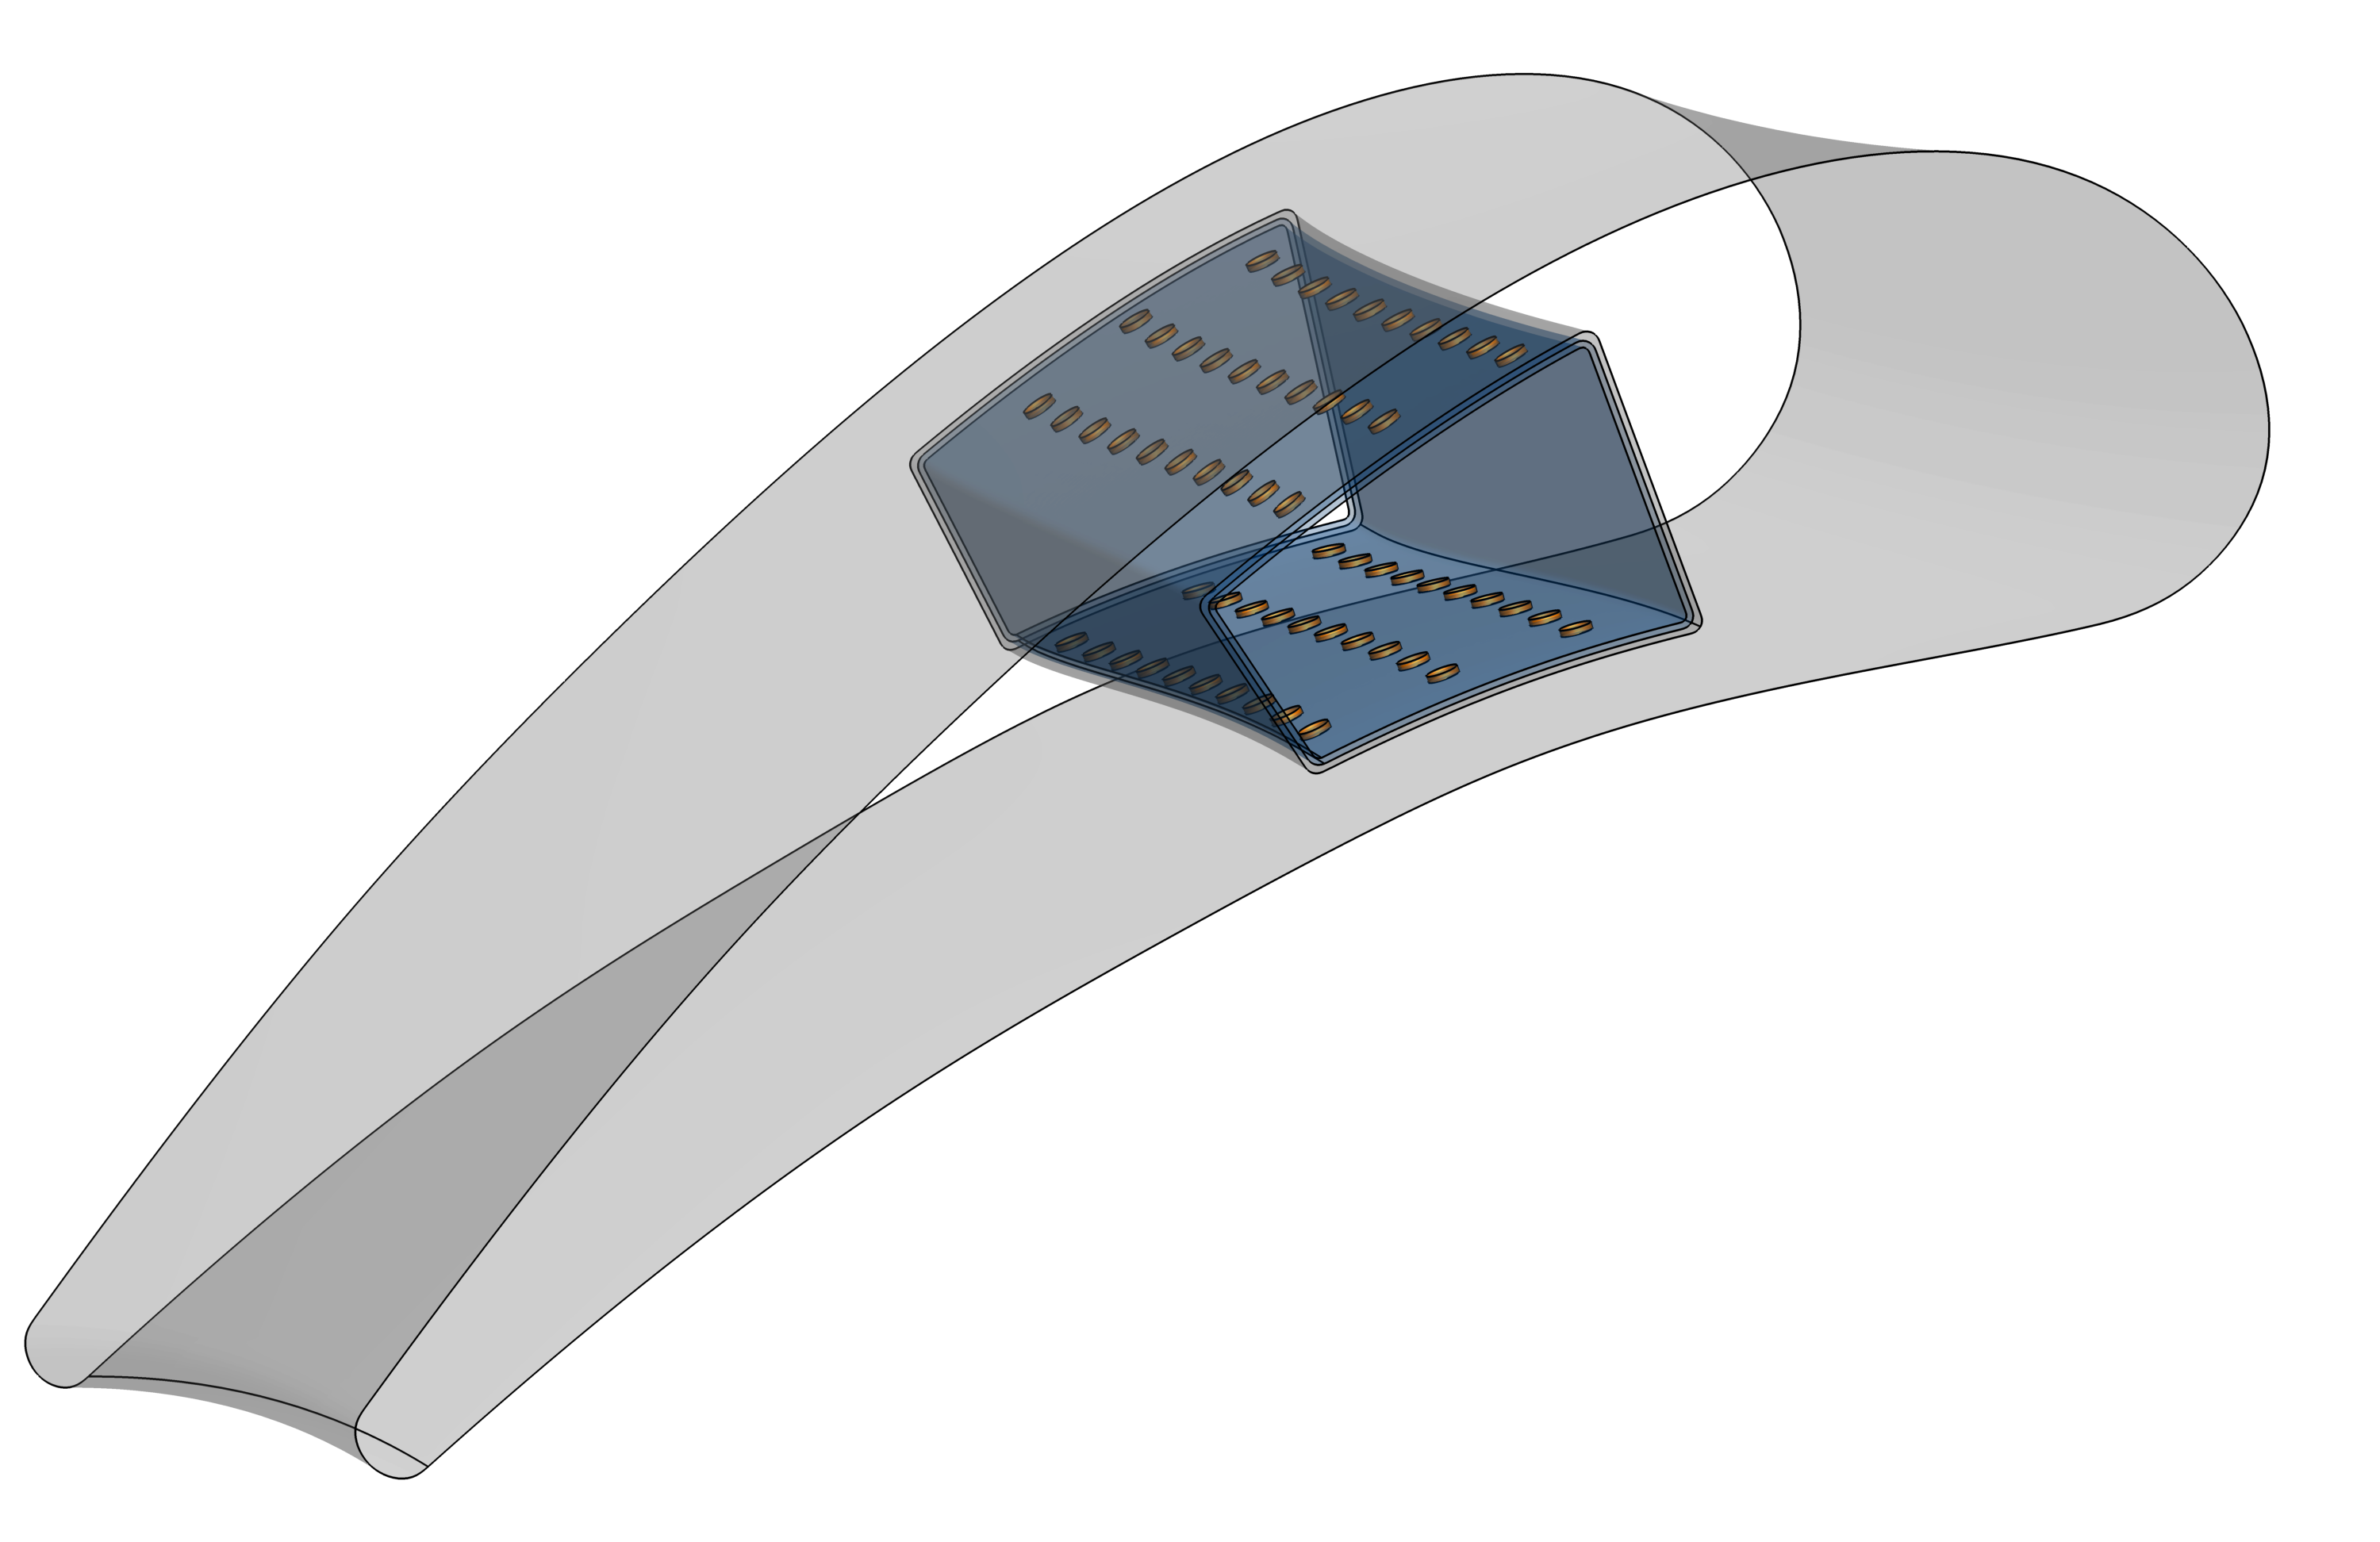
\includegraphics[width=\textwidth]{../../tec/impingement/00.png}
		\end{subfigure}
		\begin{subfigure}{.3\textwidth}
			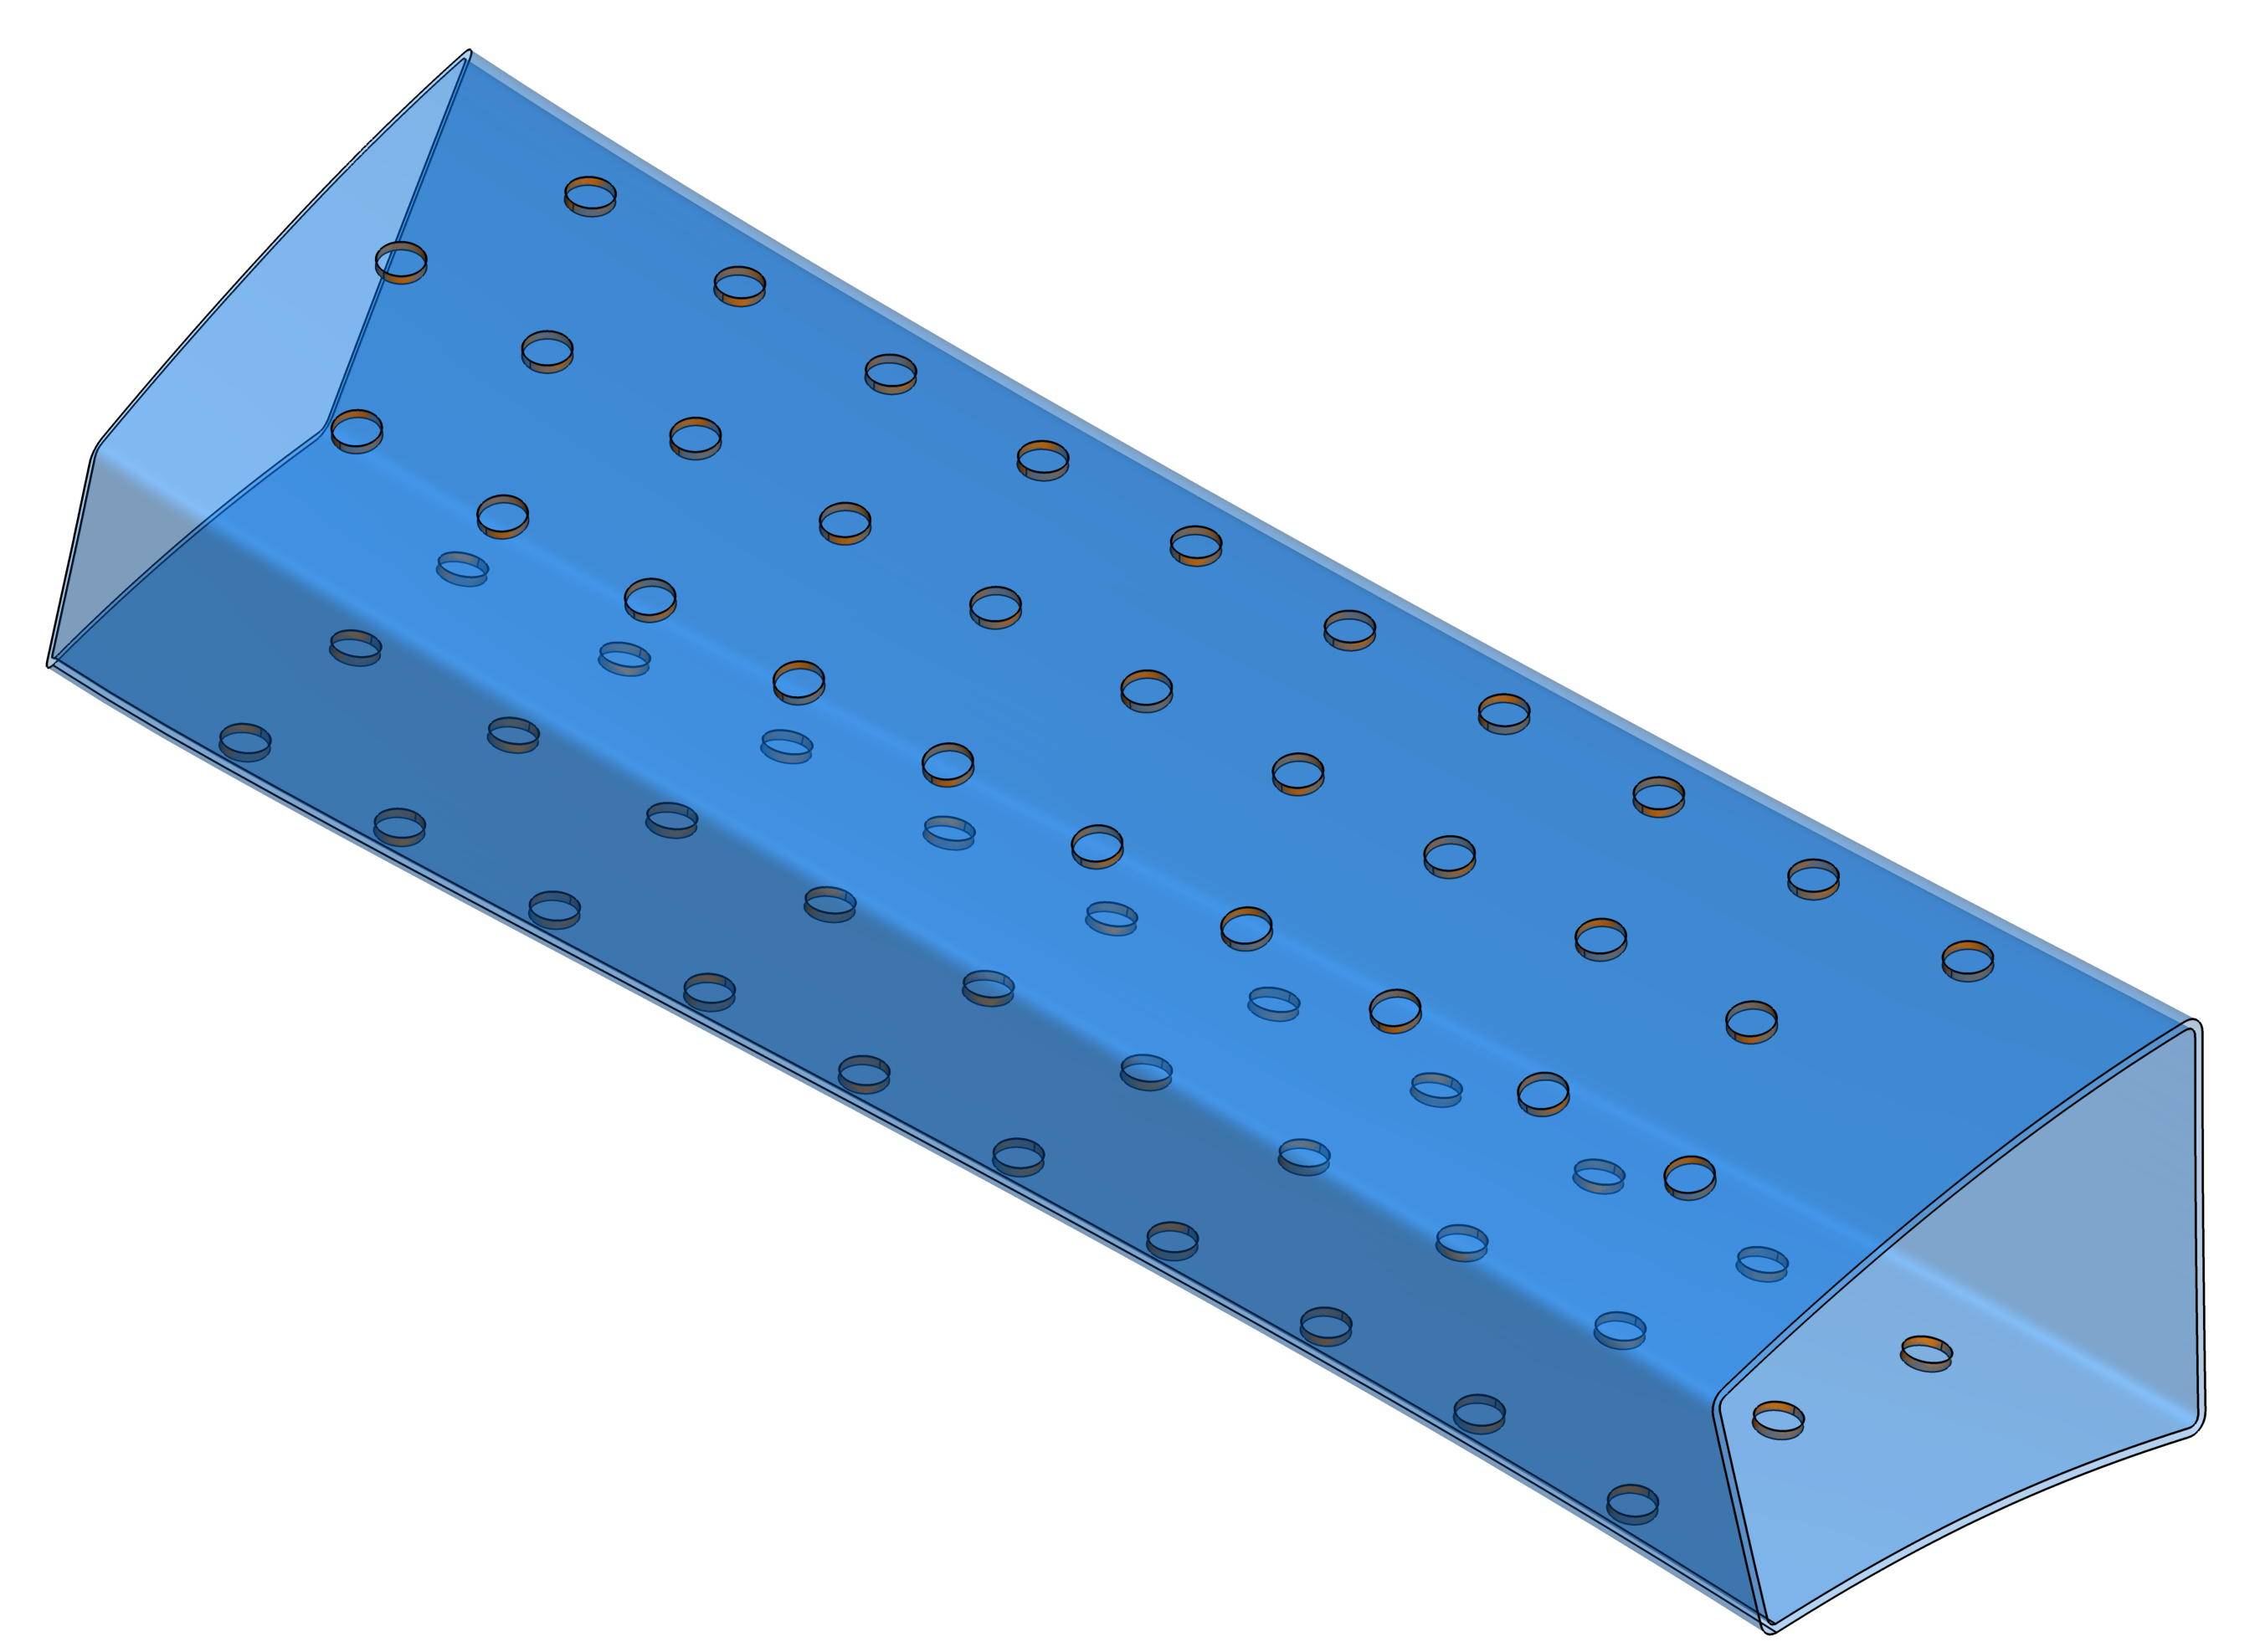
\includegraphics[width=\textwidth]{../../tec/impingement/02.png}
		\end{subfigure}
		\begin{subfigure}{.3\textwidth}
			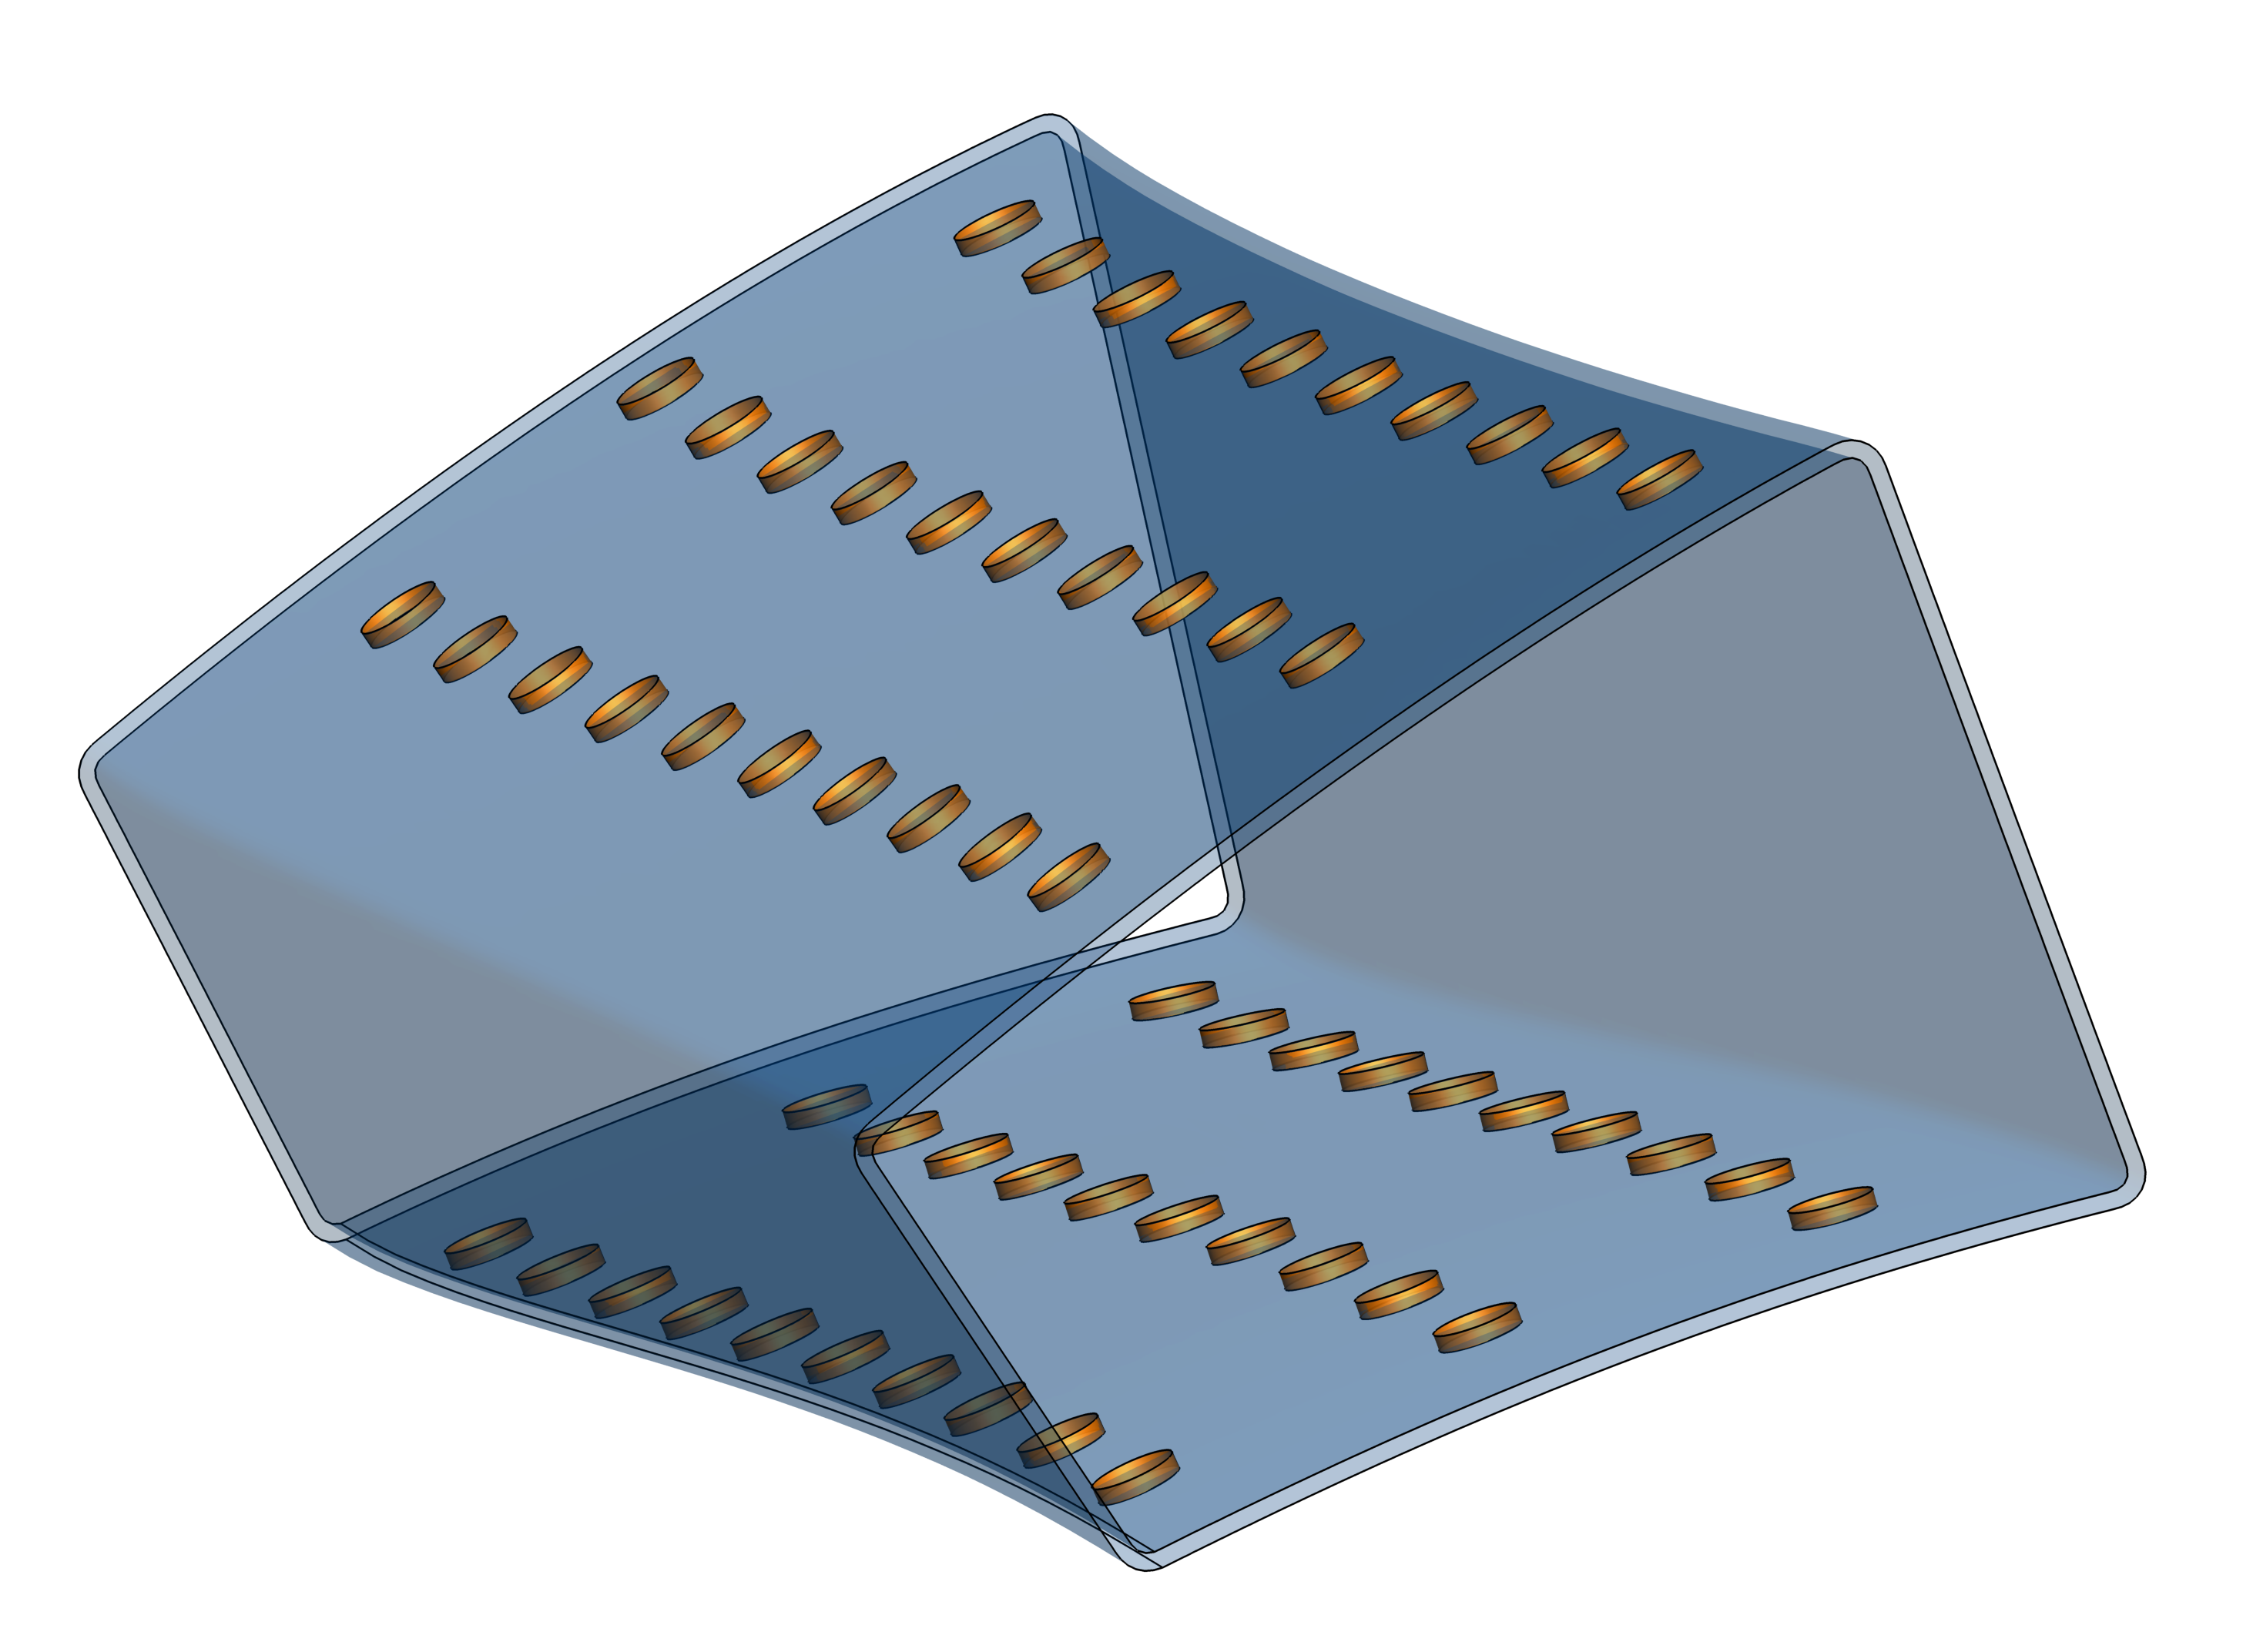
\includegraphics[width=\textwidth]{../../tec/impingement/01.png}
		\end{subfigure}
	\end{figure}
	\vfill
\end{frame}

\begin{frame}
	\frametitle{Geometrien / Prallkühlung}
	\vspace{-1cm}\hspace{-0.5cm}
	\begin{figure}[H]
		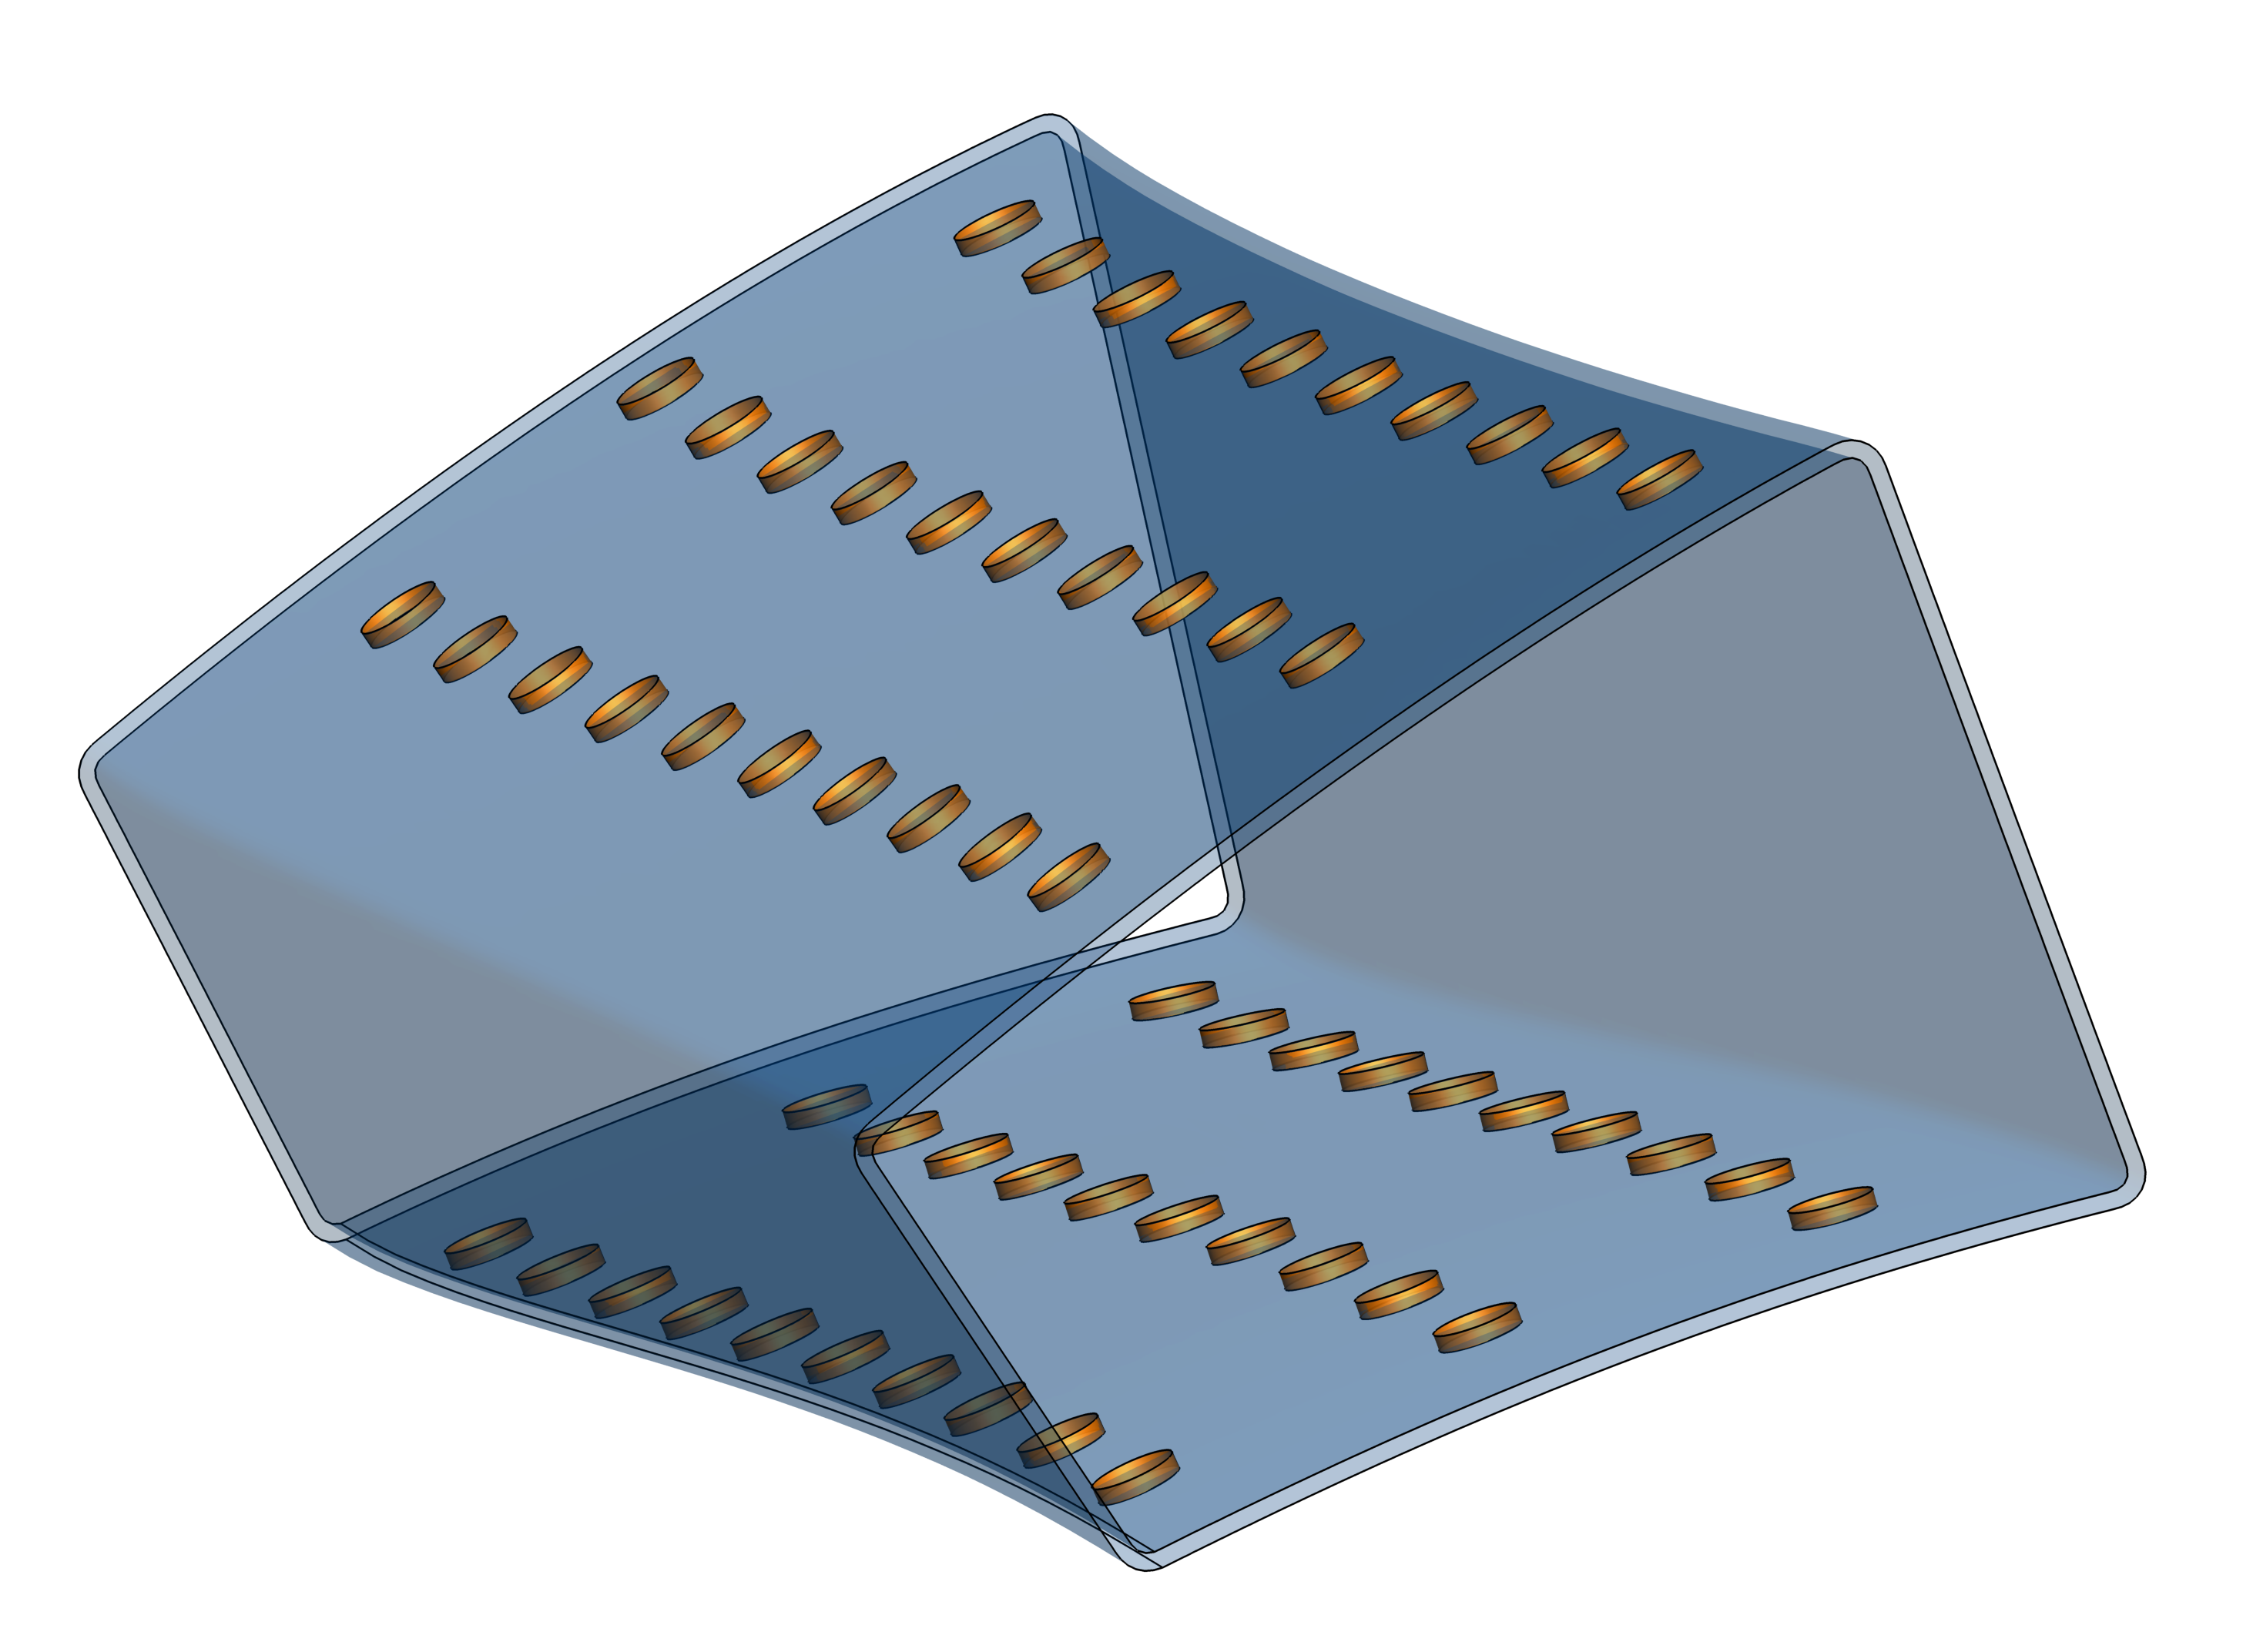
\includegraphics[width=.66\textwidth]{../../tec/impingement/01.png}
	\end{figure}
	\vfill
\end{frame}

\begin{frame}
	\frametitle{Geometrien / Prallkühlung}
	\vspace{-1cm}\hspace{-0.5cm}
	\begin{figure}[H]
		\centering
		\begin{subfigure}{.3\textwidth}
			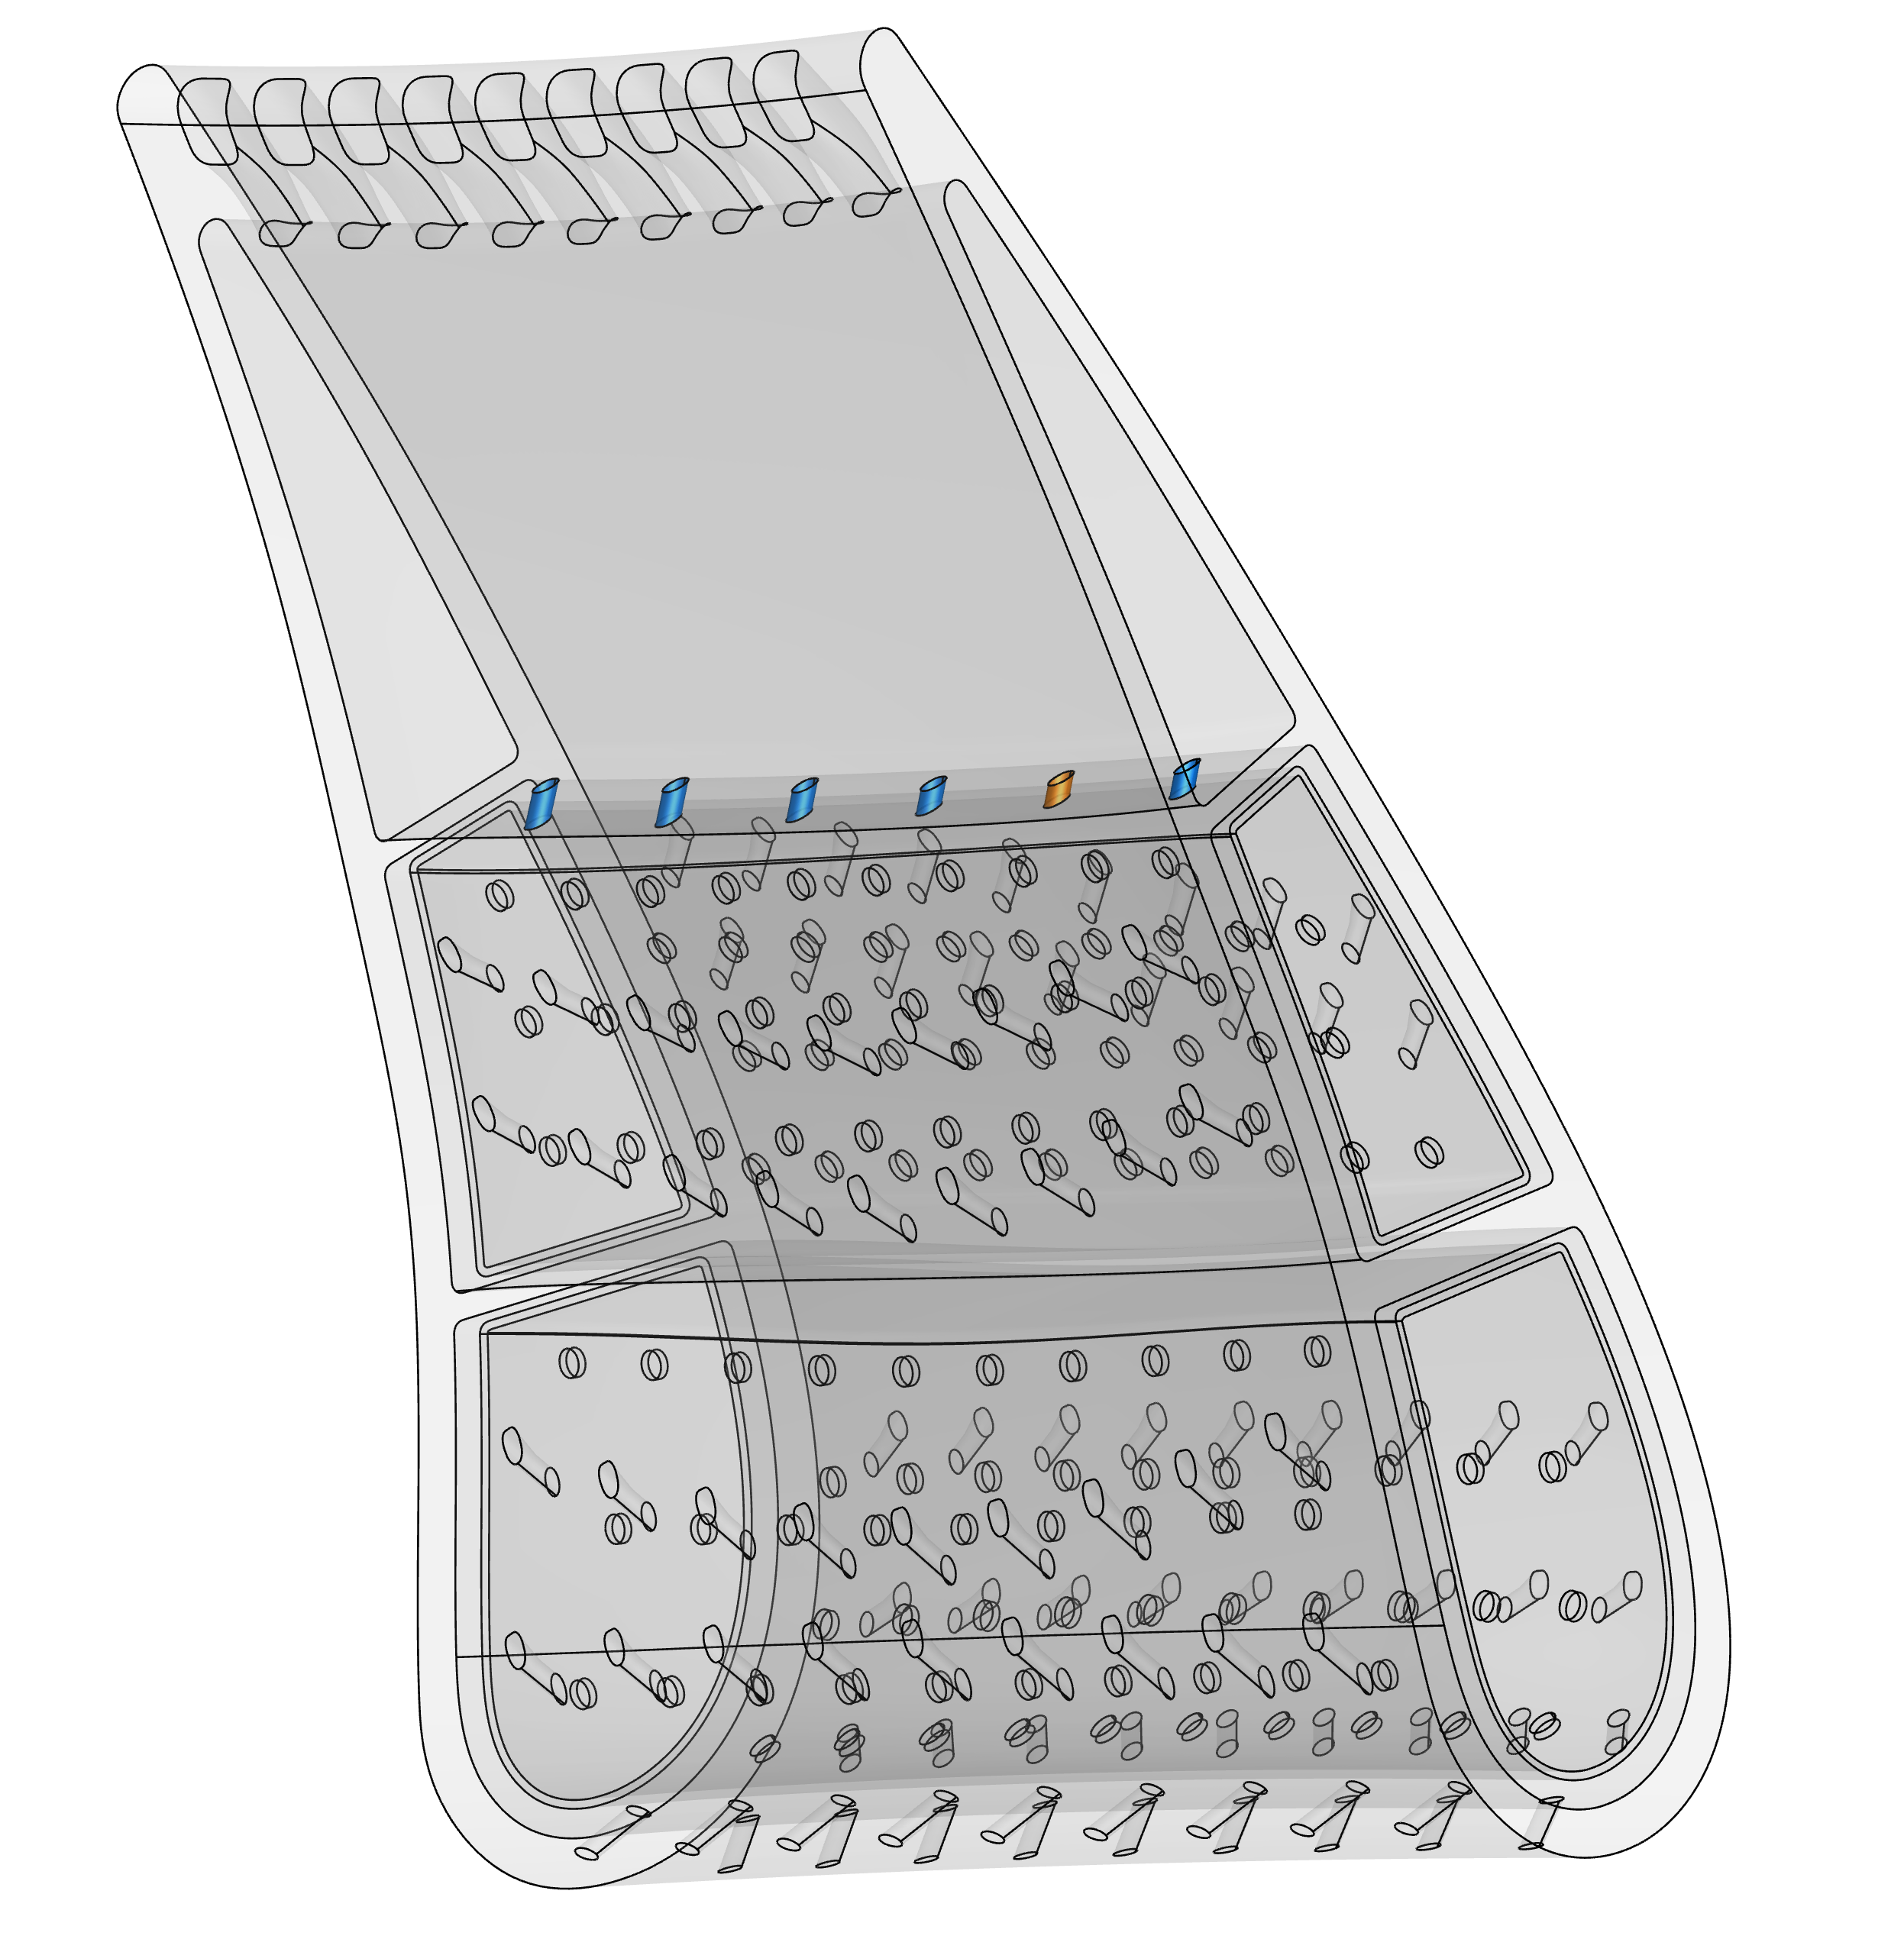
\includegraphics[width=\textwidth]{../../tec/interchannel/01.png}
		\end{subfigure}
		\begin{subfigure}{.3\textwidth}
			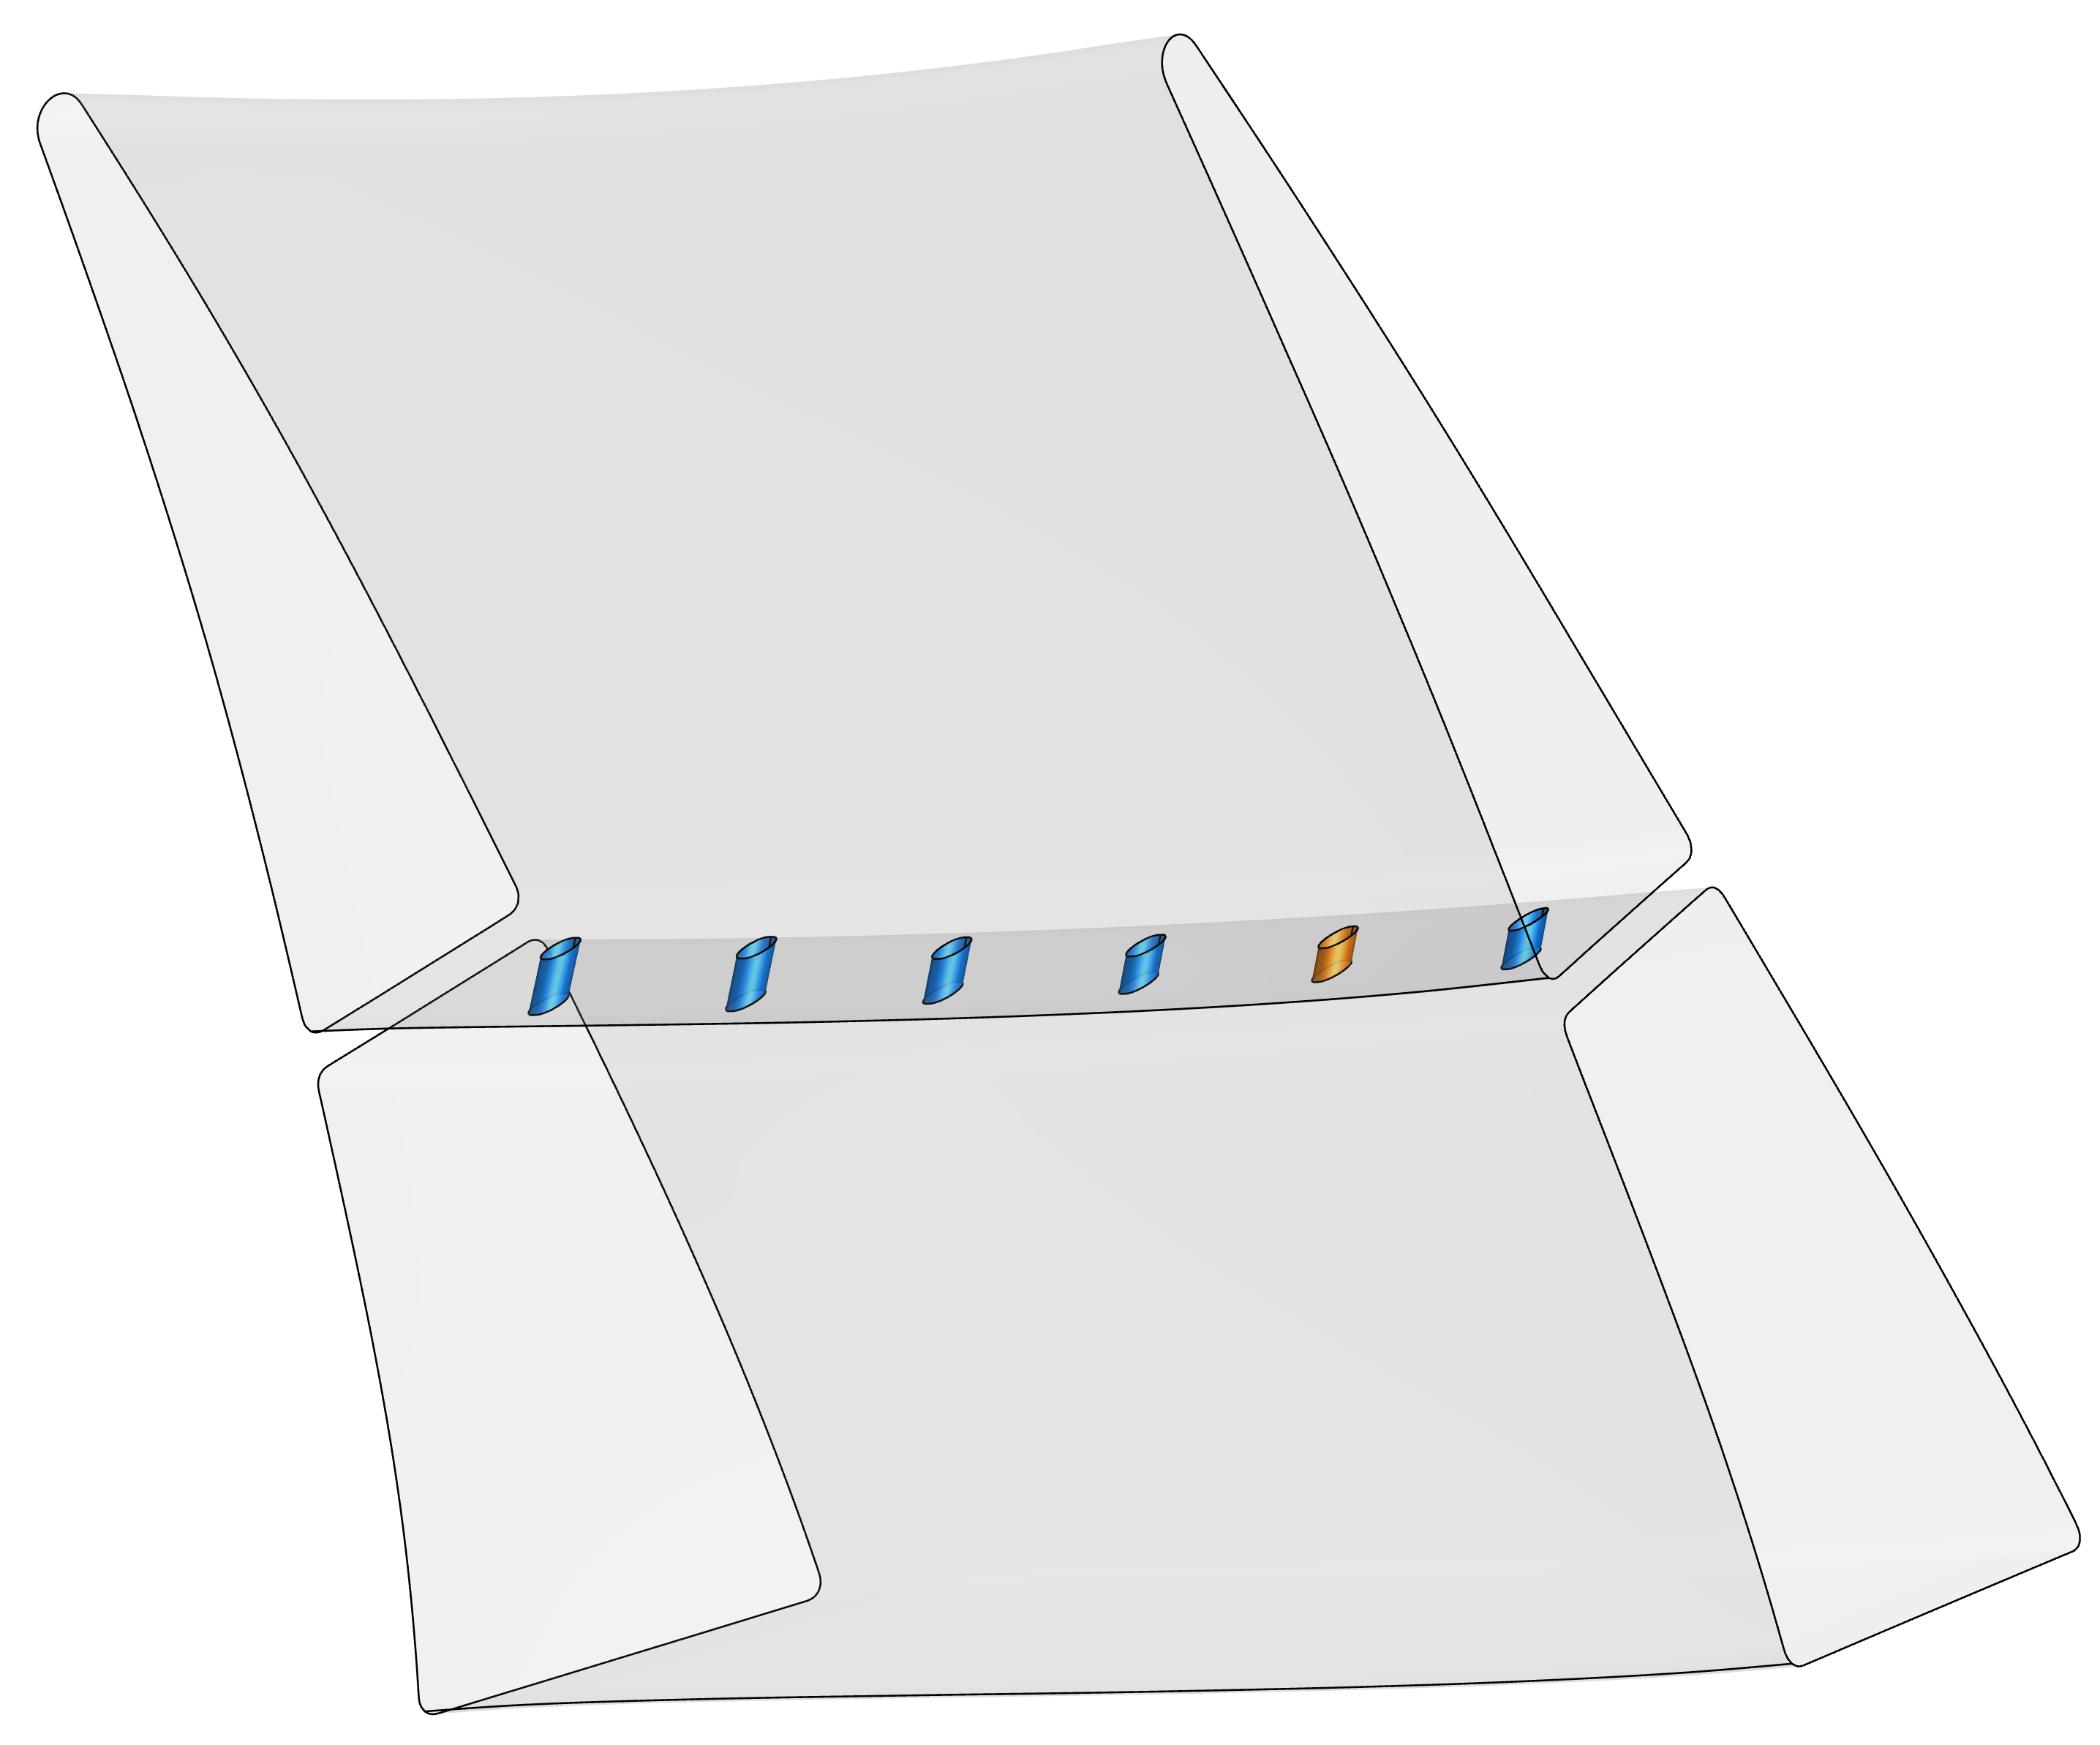
\includegraphics[width=\textwidth]{../../tec/interchannel/02.png}
		\end{subfigure}
		\begin{subfigure}{.3\textwidth}
			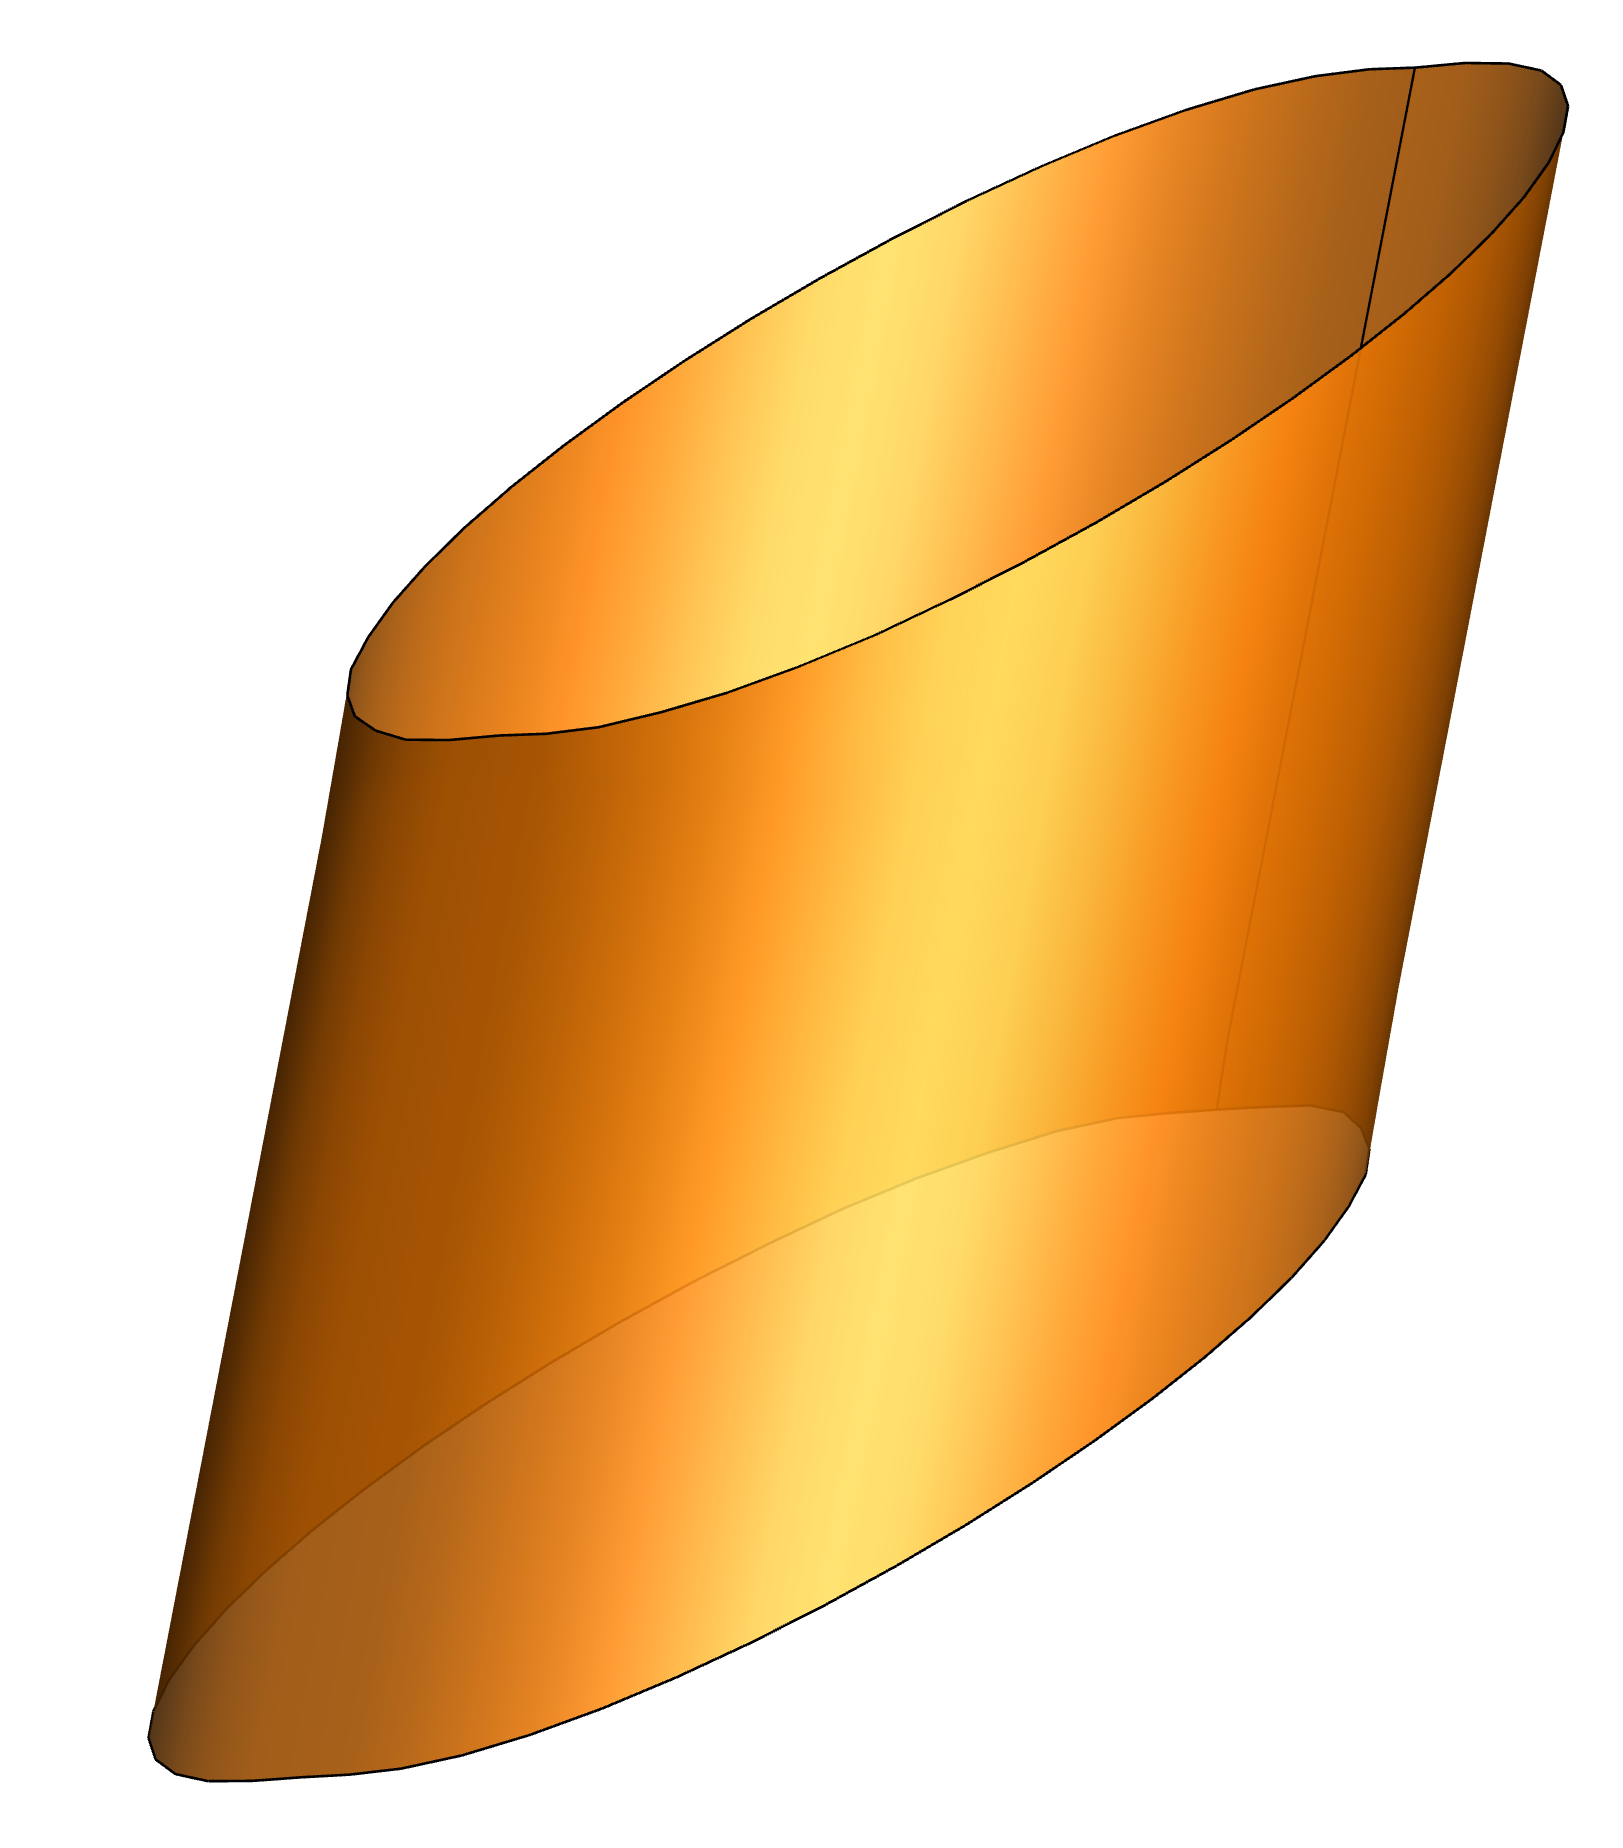
\includegraphics[width=\textwidth]{../../tec/interchannel/03.png}
		\end{subfigure}
	\end{figure}
	\vfill
\end{frame}

\begin{frame}
	\frametitle{Geometrien / Überblick}
	\vspace{-1.5cm}\hspace{-0.5cm}
	\begin{minipage}[t]{0.38\textwidth}
		\begin{itemize}
			\item[\ding{108}] Kühlkanäle
			\item[\ding{108}] Filmkühlung
			\item[\ding{108}] Prallkühlung
			\item[\ding{109}] Ausblasungsschlitze
			\item[\ding{109}] Pin-fins
		\end{itemize}
	\end{minipage}
	\begin{minipage}{0.6\textwidth}
		\begin{figure}[H]
			\centering
			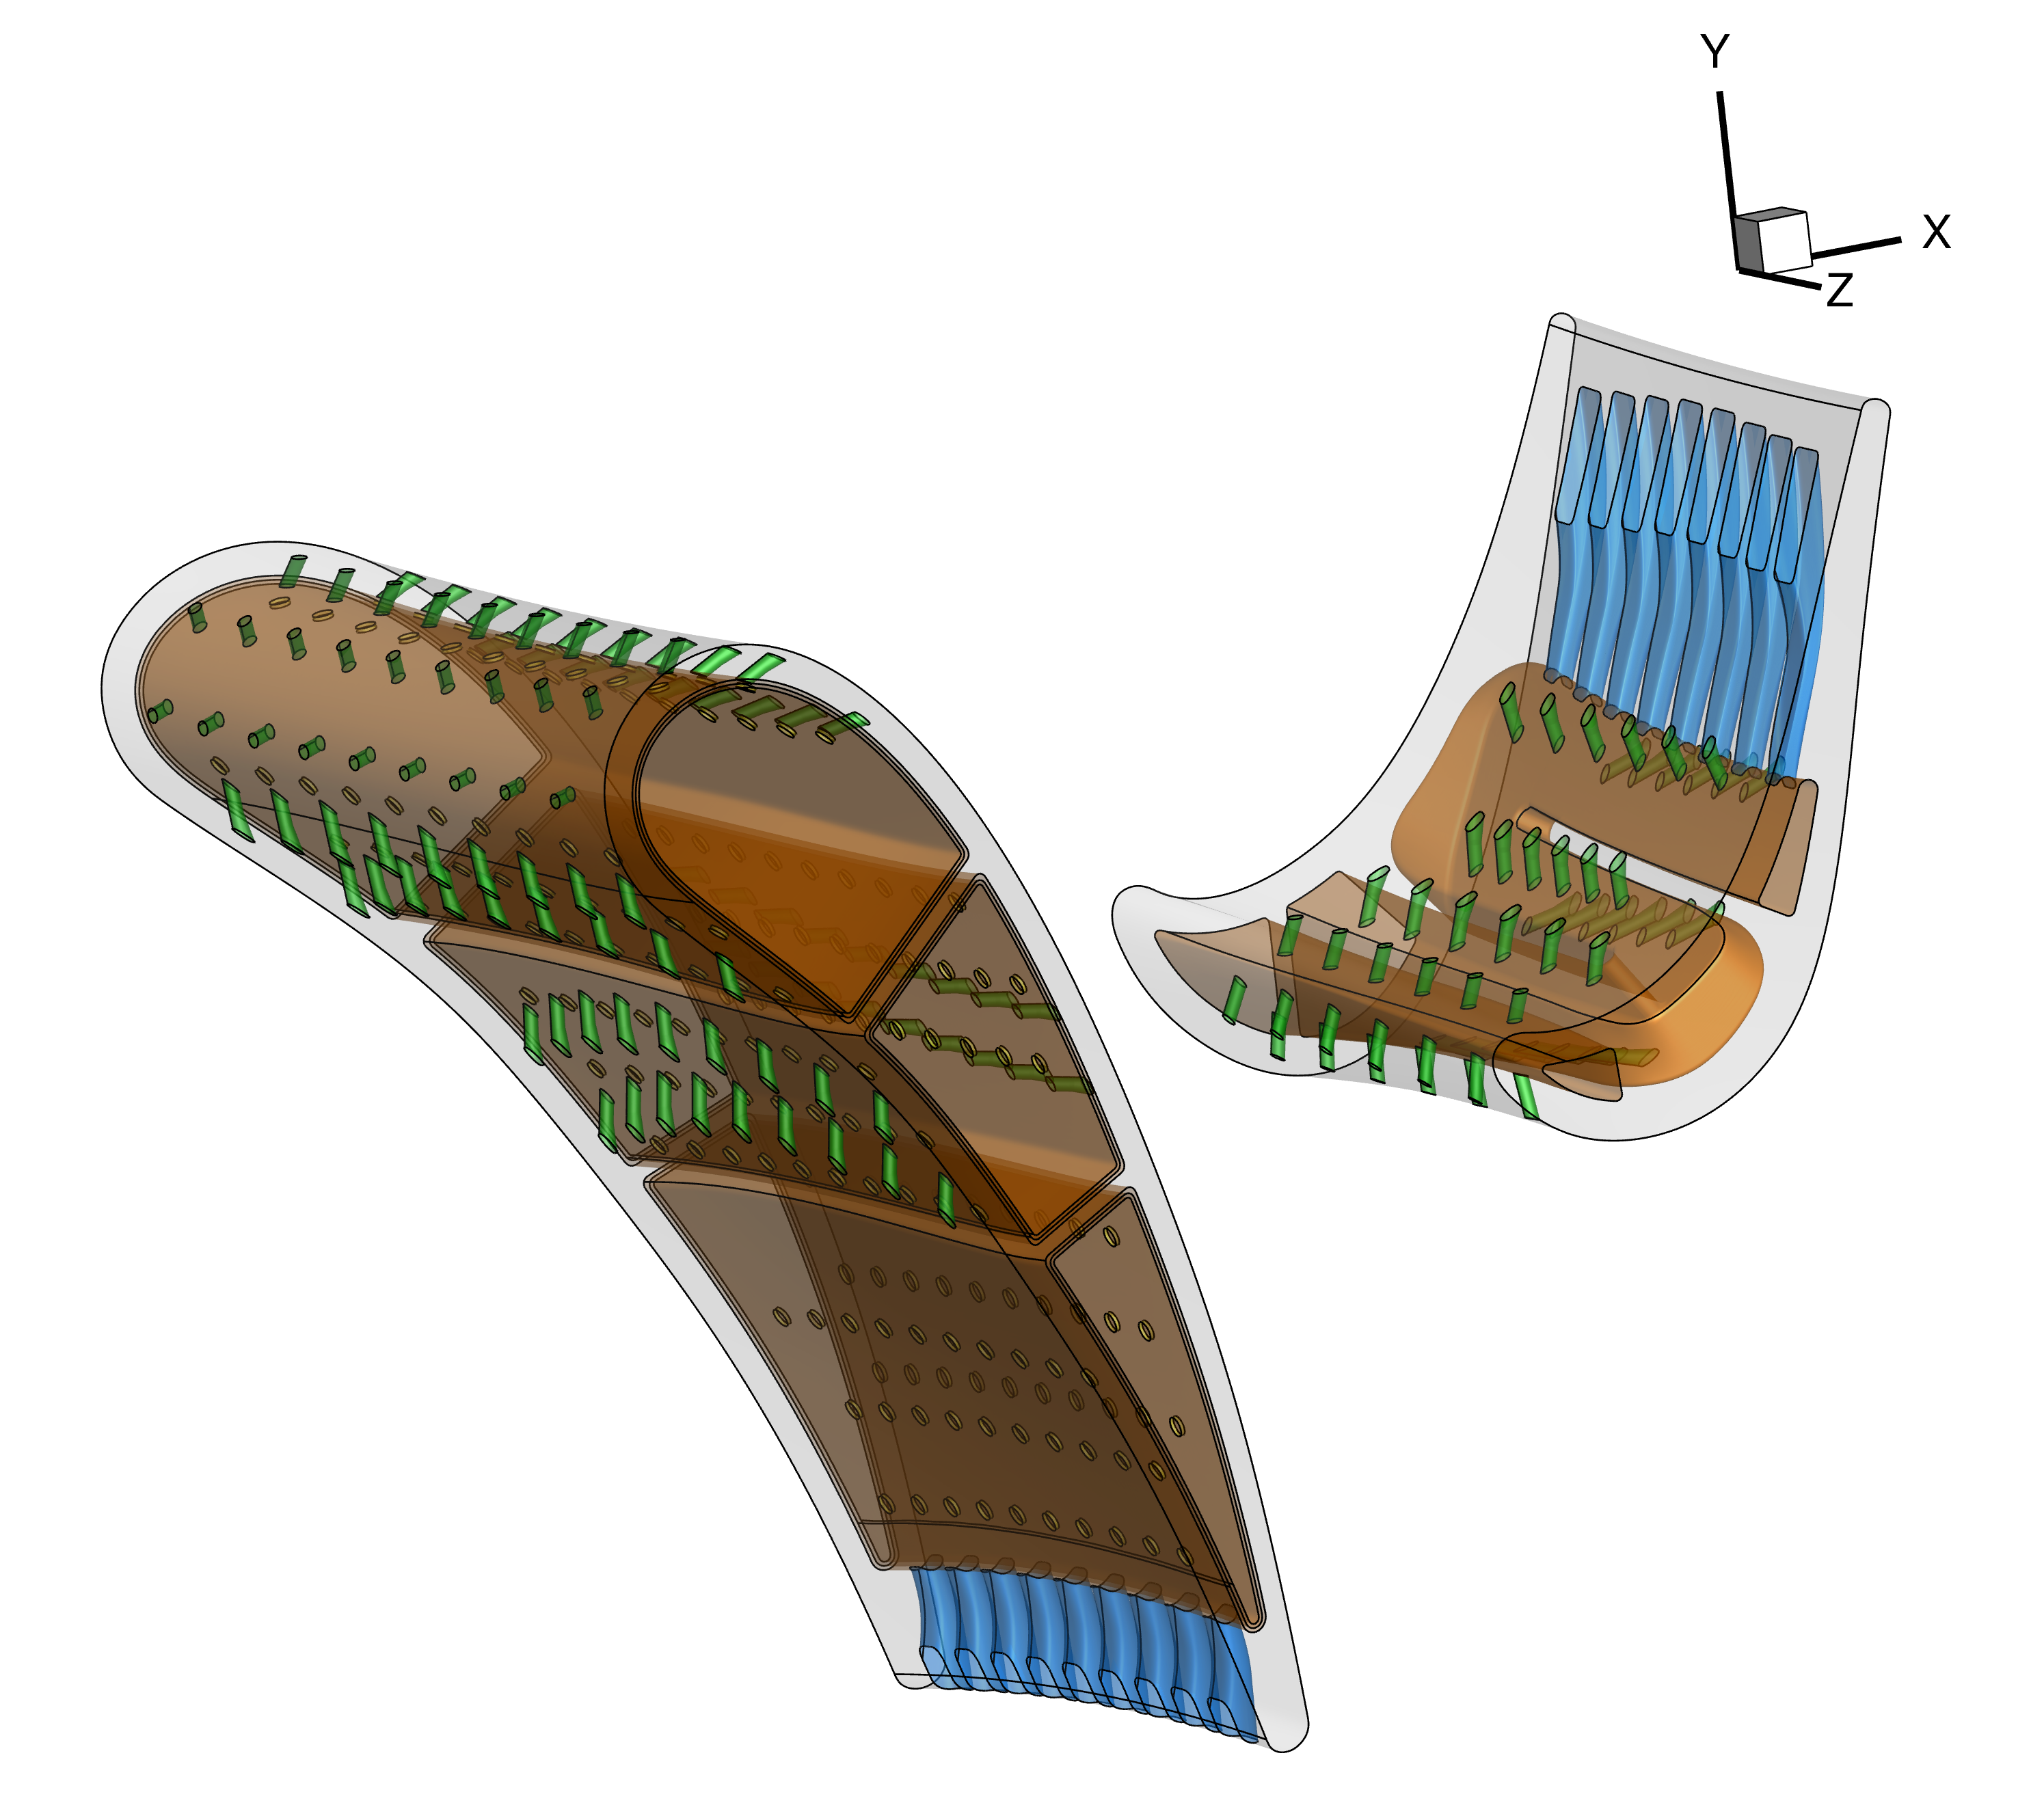
\includegraphics[width=\textwidth]{../../tec/complete/60.png}
		\end{figure}
	\end{minipage}
	\vfill
\end{frame}

\begin{frame}
	\frametitle{Geometrien / Überblick}
	\vspace{-1.5cm}\hspace{-0.5cm}
	\begin{minipage}[t]{0.38\textwidth}
		\begin{itemize}
			\item[\ding{108}] Kühlkanäle
			\item[\ding{108}] Filmkühlung
			\item[\ding{108}] Prallkühlung
			\item[\ding{40}] Ausblasungsschlitze
			\item[\ding{109}] Pin-fins
		\end{itemize}
	\end{minipage}
	\begin{minipage}{0.6\textwidth}
		\begin{figure}[H]
			\centering
			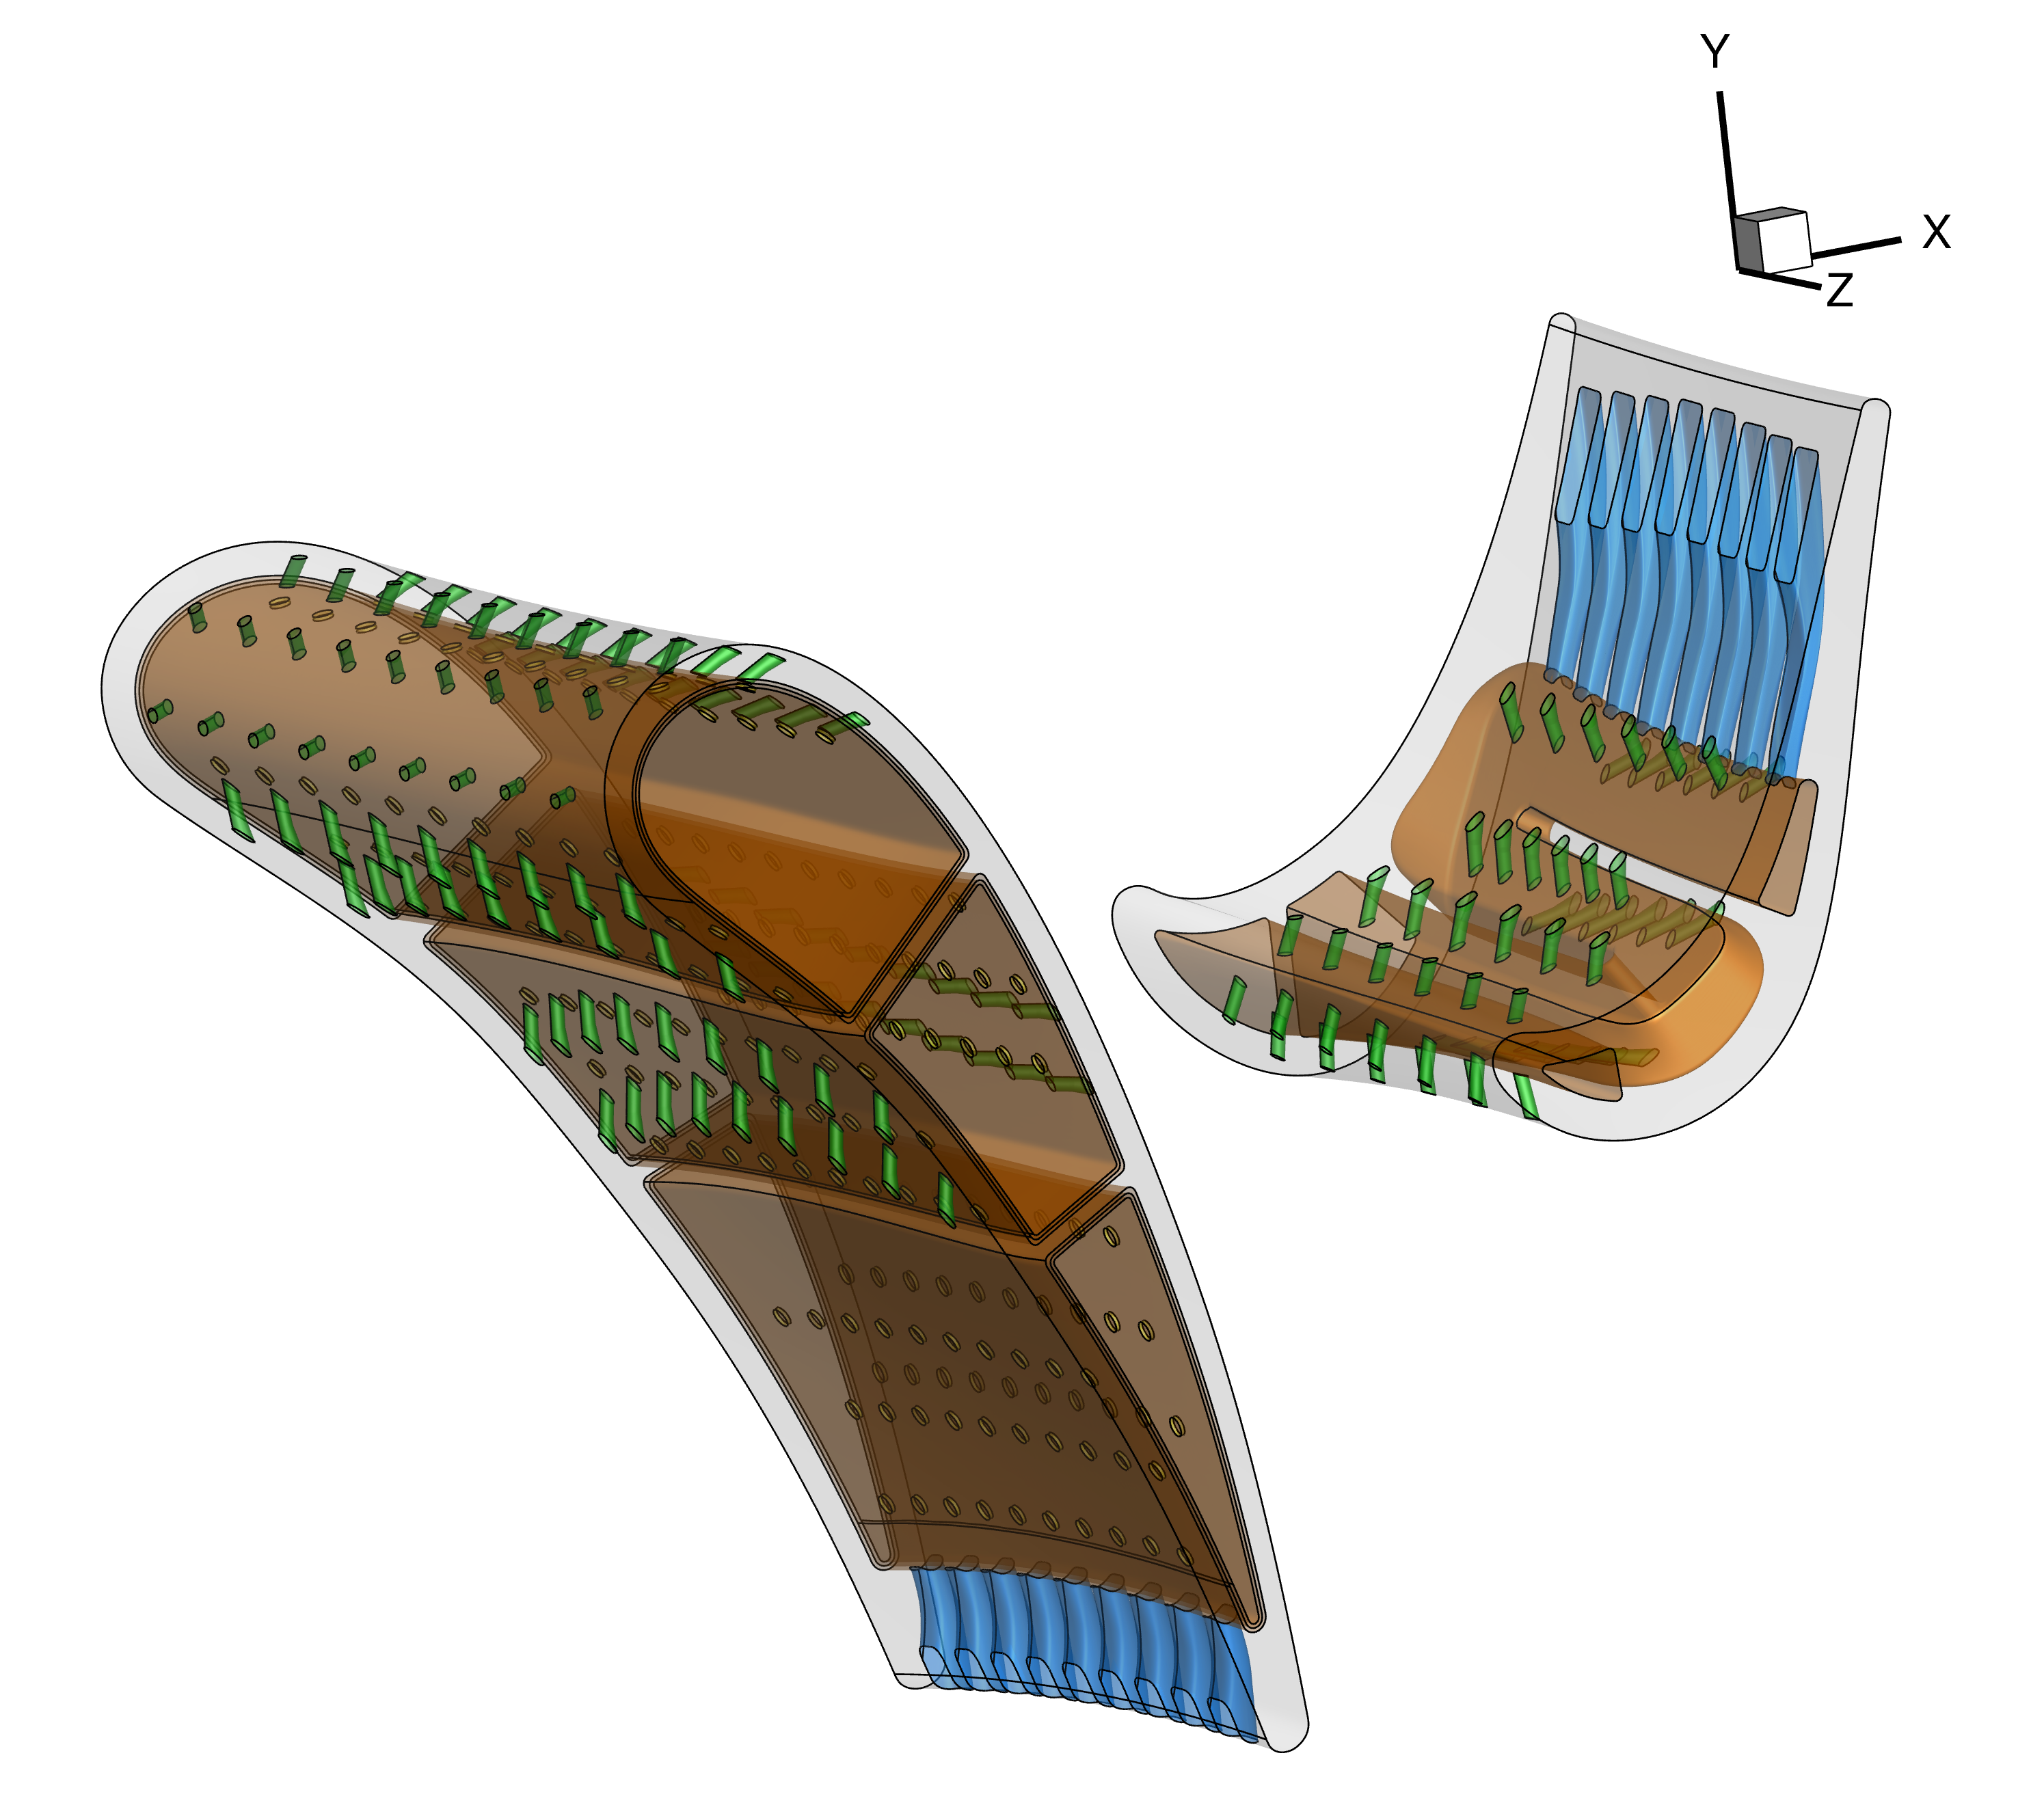
\includegraphics[width=\textwidth]{../../tec/complete/60.png}
		\end{figure}
	\end{minipage}
	\vfill
\end{frame}

\begin{frame}
	\frametitle{Geometrien / Slots}
	\vspace{0cm}\hspace{-0.5cm}
	\begin{figure}[H]
		\centering
		\begin{subfigure}{.45\textwidth}
			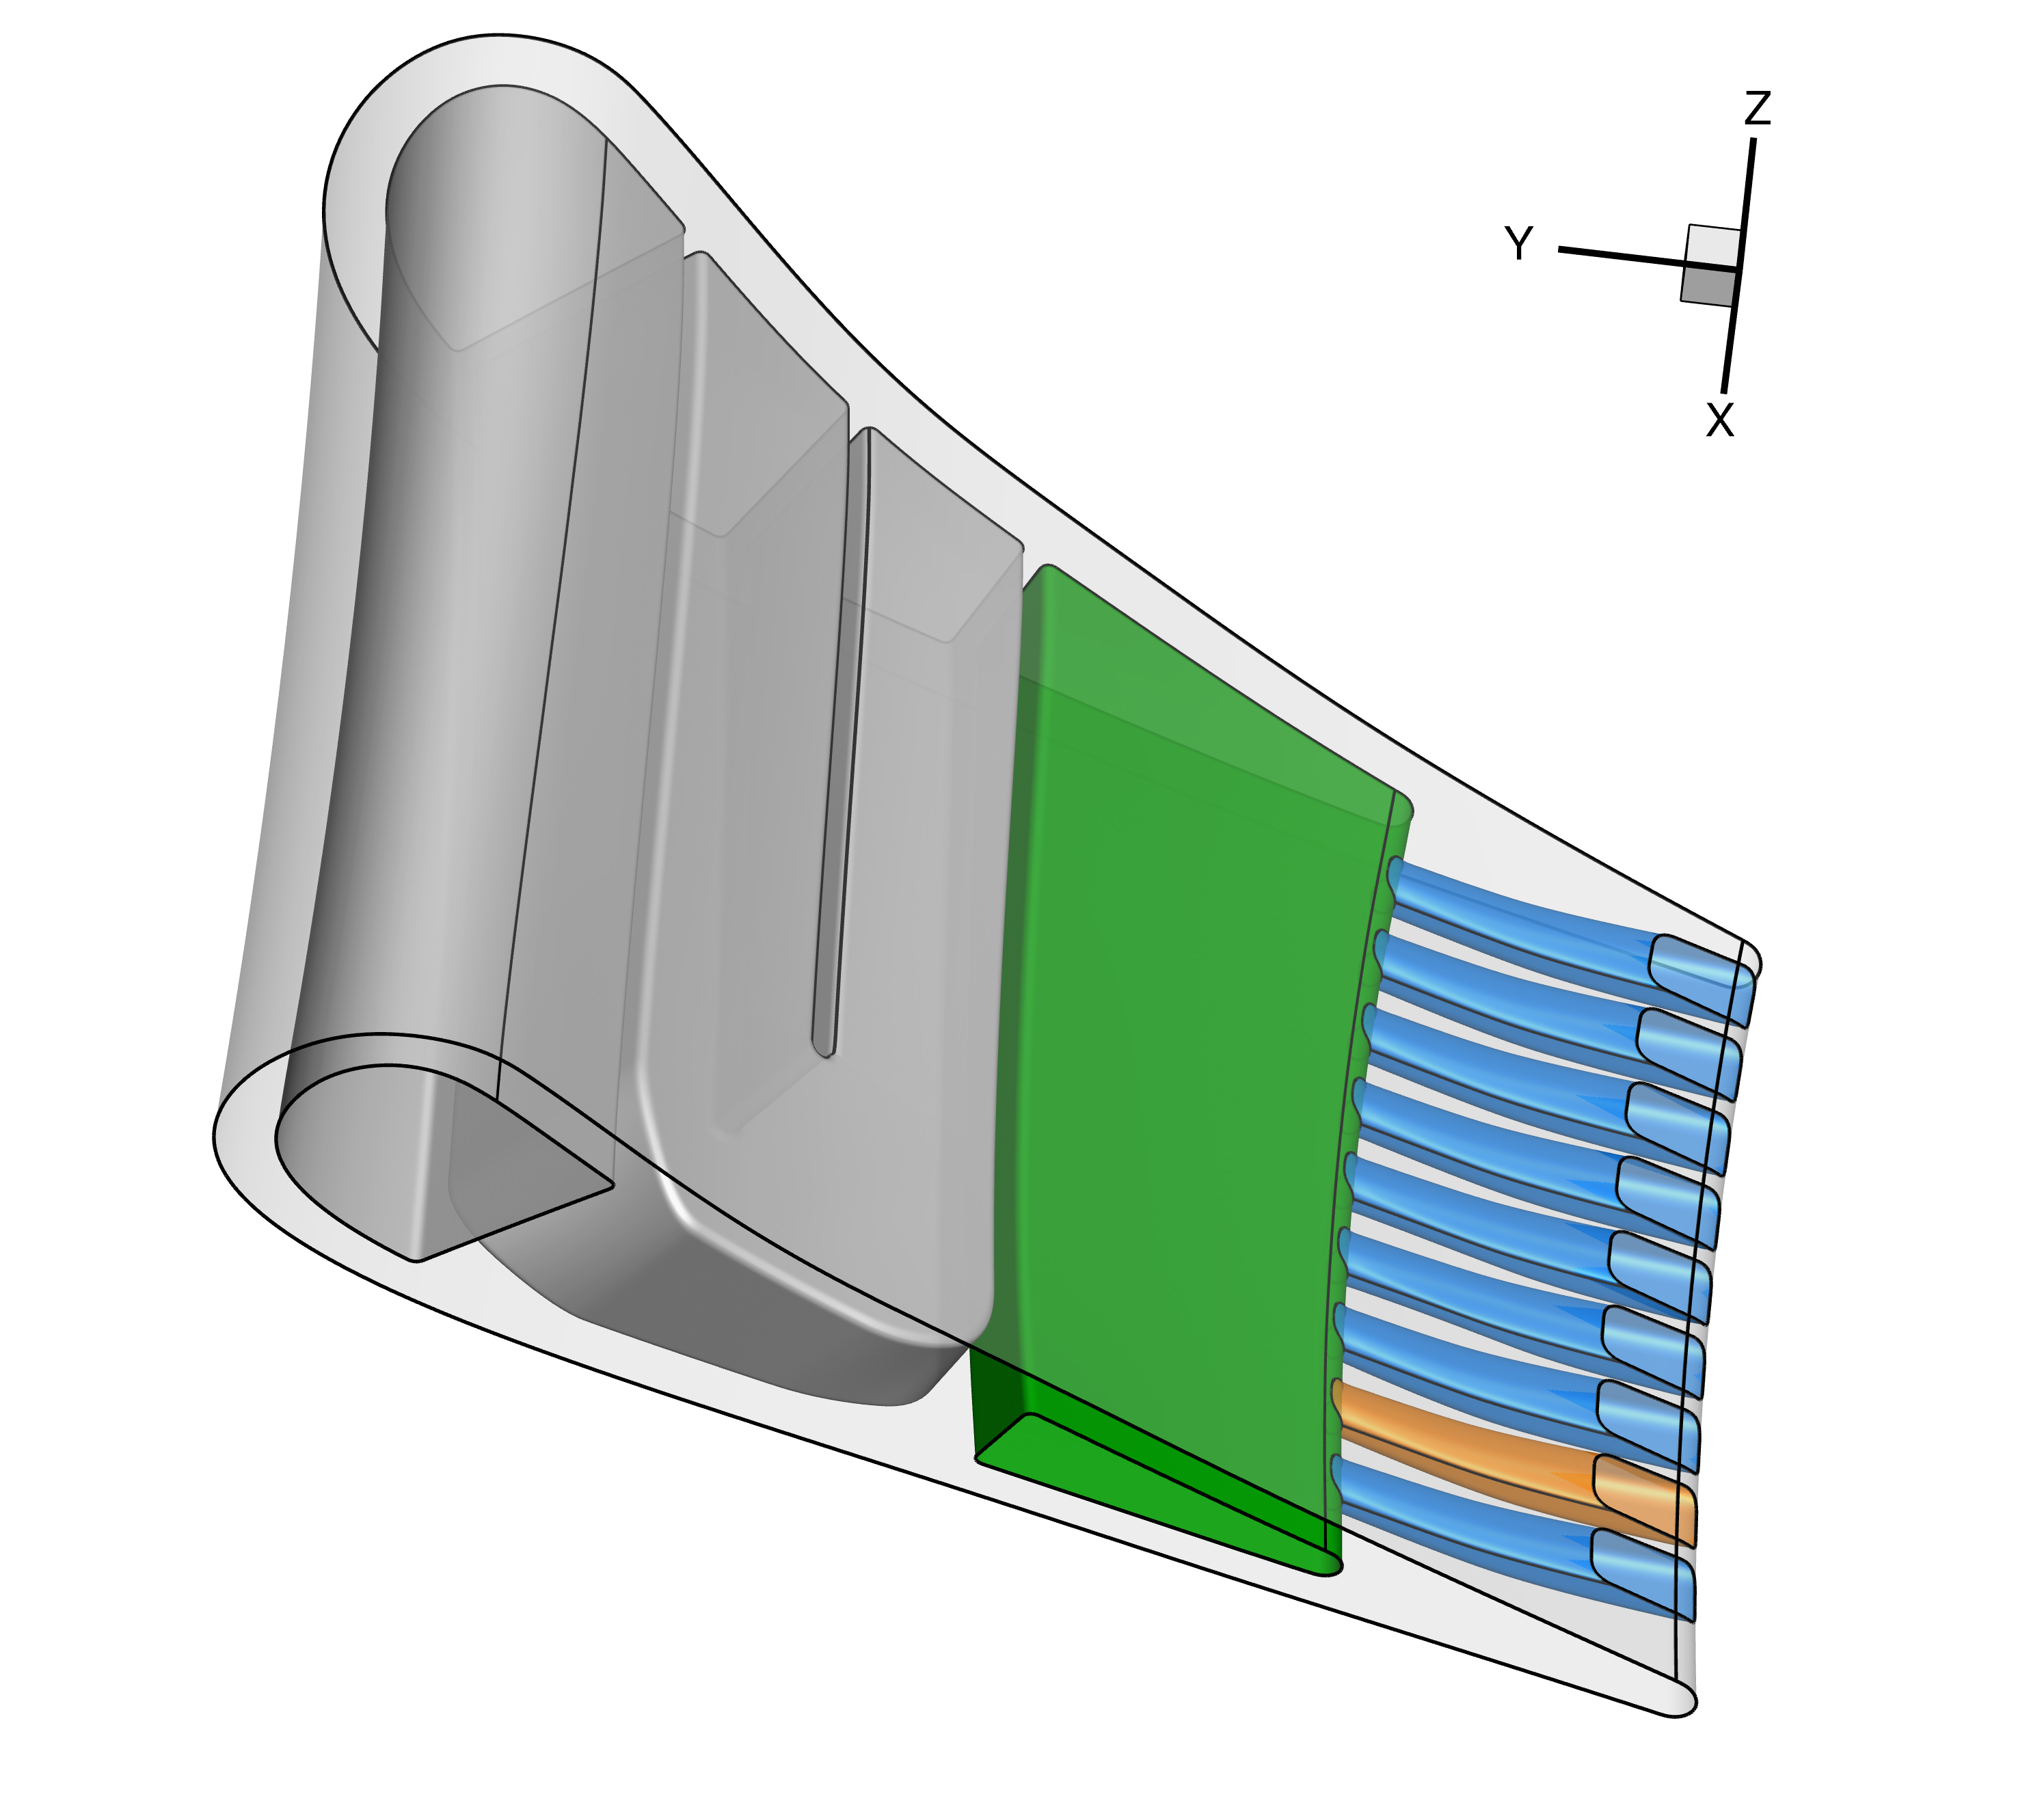
\includegraphics[width=\textwidth]{../../tec/slots/11.png}
		\end{subfigure}
		\phantom{aaa}
		\begin{subfigure}{.45\textwidth}
			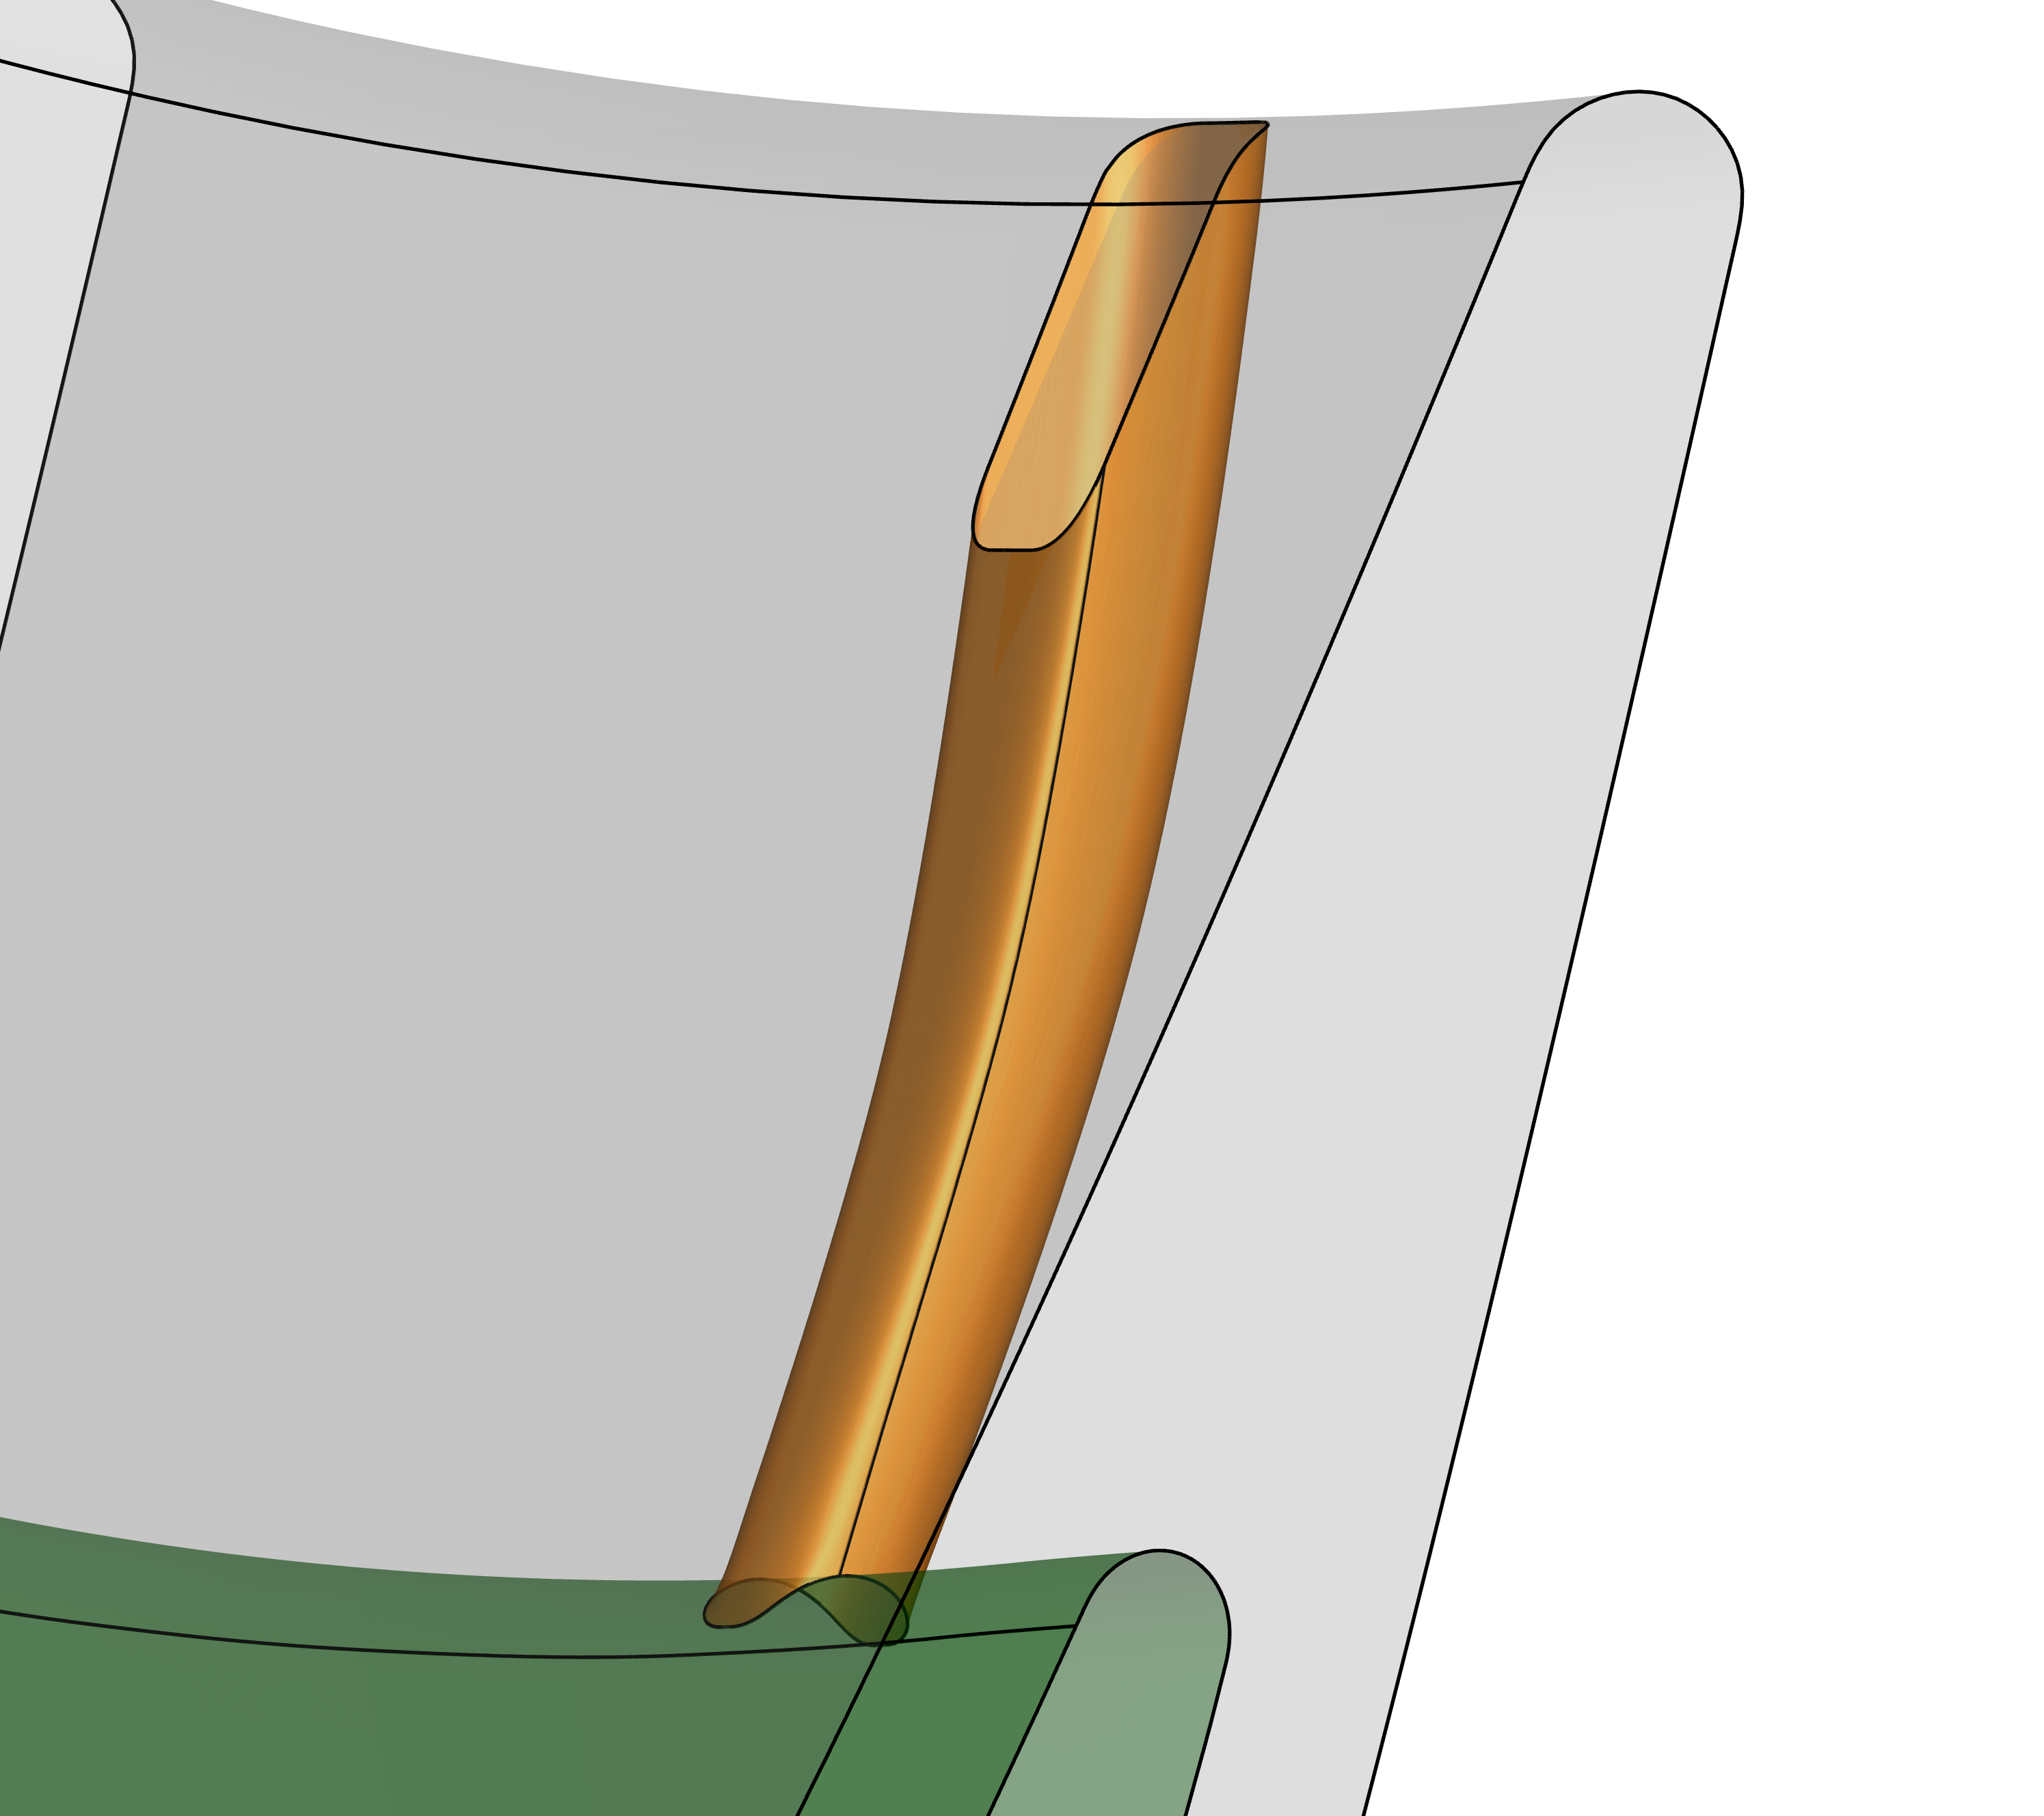
\includegraphics[width=\textwidth]{../../tec/slots/12.png}
		\end{subfigure}
	\end{figure}
	\vfill
\end{frame}

\begin{frame}
	\frametitle{Geometrien / Slots}
	\vspace{0cm}\hspace{-0.5cm}
	\begin{figure}[H]
		\centering
		\begin{subfigure}{.45\textwidth}
			\includegraphics[width=\textwidth]{../../tec/slots/15.png}
		\end{subfigure}
		\phantom{aaa}
		\begin{subfigure}{.45\textwidth}
			\includegraphics[width=\textwidth]{../../tec/slots/14.png}
		\end{subfigure}
	\end{figure}
	\vfill
\end{frame}

\begin{frame}
	\frametitle{Geometrien / Slots}
	\vspace{-1cm}\hspace{-0.5cm}
	\begin{figure}[H]
		\centering
		\begin{subfigure}{.3\textwidth}
			\includegraphics[width=\textwidth]{../../tec/slots/16.png}
		\end{subfigure}
		\begin{subfigure}{.3\textwidth}
			\includegraphics[width=\textwidth]{../../tec/slots/17.png}
		\end{subfigure}
		\begin{subfigure}{.3\textwidth}
			\includegraphics[width=\textwidth]{../../tec/slots/18.png}
		\end{subfigure}
	\end{figure}
	\vfill
\end{frame}

\begin{frame}
	\frametitle{Geometrien / Überblick}
	\vspace{-1.5cm}\hspace{-0.5cm}
	\begin{minipage}[t]{0.38\textwidth}
		\begin{itemize}
			\item[\ding{108}] Kühlkanäle
			\item[\ding{108}] Filmkühlung
			\item[\ding{108}] Prallkühlung
			\item[\ding{108}] Ausblasungsschlitze
			\item[\ding{109}] Pin-fins
		\end{itemize}
	\end{minipage}
	\begin{minipage}{0.6\textwidth}
		\begin{figure}[H]
			\centering
			\includegraphics[width=\textwidth]{../../tec/complete/60.png}
		\end{figure}
	\end{minipage}
	\vfill
\end{frame}

\begin{frame}
	\frametitle{Geometrien / Überblick}
	\vspace{-1.5cm}\hspace{-0.5cm}
	\begin{minipage}[t]{0.38\textwidth}
		\begin{itemize}
			\item[\ding{108}] Kühlkanäle
			\item[\ding{108}] Filmkühlung
			\item[\ding{108}] Prallkühlung
			\item[\ding{108}] Ausblasungsschlitze
			\item[\ding{40}] Pin-fins
		\end{itemize}
	\end{minipage}
	\begin{minipage}{0.6\textwidth}
		\begin{figure}[H]
			\centering
			\includegraphics[width=\textwidth]{../../tec/complete/60.png}
		\end{figure}
	\end{minipage}
	\vfill
\end{frame}

\begin{frame}
	\frametitle{Geometrien / Pin-fins}
	\vspace{-1cm}\hspace{-0.5cm}
	\begin{figure}[H]
		\centering
		\begin{subfigure}{.3\textwidth}
			\includegraphics[width=\textwidth]{../../tec/pinfin/10.png}
		\end{subfigure}
		\begin{subfigure}{.3\textwidth}
			\includegraphics[width=\textwidth]{../../tec/pinfin/11.png}
		\end{subfigure}
		\begin{subfigure}{.3\textwidth}
			\includegraphics[width=\textwidth]{../../tec/pinfin/12.png}
		\end{subfigure}
	\end{figure}
	\vfill
\end{frame}

\begin{frame}
	\frametitle{Geometrien / Überblick}
	\vspace{-1.5cm}\hspace{-0.5cm}
	\begin{minipage}[t]{0.38\textwidth}
		\begin{itemize}
			\item[\ding{108}] Kühlkanäle
			\item[\ding{108}] Filmkühlung
			\item[\ding{108}] Prallkühlung
			\item[\ding{108}] Ausblasungsschlitze
			\item[\ding{108}] Pin-fins
		\end{itemize}
	\end{minipage}
	\begin{minipage}{0.6\textwidth}
		\begin{figure}[H]
			\centering
			\includegraphics[width=\textwidth]{../../tec/complete/60.png}
		\end{figure}
	\end{minipage}
	\vfill
\end{frame}

\begin{frame}
	\frametitle{Nutzung}
	\vspace{-1.5cm}\hspace{-0.5cm}
	\begin{minipage}[t]{0.38\textwidth}
		\vspace{-2cm}
		\begin{itemize}
			\item[\ding{109}] Prozesskette
			\item[\ding{109}] Vollkörpererzeugung
			\item[\ding{109}] CFD mit TRACE
		\end{itemize}
	\end{minipage}
	\begin{minipage}{0.6\textwidth}
		\begin{figure}[H]
			\centering
			\vspace{1cm}
			\includegraphics[width=\textwidth, trim={5px 5px 5px 5px}, clip]{../../assets/solid/surfaces2.png}
		\end{figure}
	\end{minipage}
	\vfill
\end{frame}

\begin{frame}
	\frametitle{Prozesskette}
	\vspace{-1cm}\hspace{-0.5cm}
	\begin{figure}[H]
		\centering
		\begin{tikzpicture}[font=\small]
			\node[draw, rounded rectangle, minimum width=2cm, minimum height=1cm] (GTlab) 							{Input performance data};
			\node[draw, rectangle, minimum width=2.5cm, minimum height=1cm, left=of GTlab] (PrEDiCT) 				{\textbf{PrEDiCT}};
			\node[draw, rectangle, minimum width=2cm, minimum height=1cm, left=of PrEDiCT] (BladeGen)				{\textbf{BladeGen}};
			\node[minimum width=2.5cm, minimum height=1cm, below=of BladeGen] (spacer)								{};
			\node[draw, rectangle, minimum width=2cm, minimum height=1cm, below=of spacer] (MISES)					{\textbf{MISES}};
			\node[draw, rectangle, minimum width=2cm, minimum height=1cm, right=of MISES] (PICCOOLO)				{\textbf{PICCOOLO}};
			\node[draw, rounded rectangle, minimum width=2cm, minimum height=1cm, above=of PICCOOLO] (2DGeom)		{2D geometry};
			\node[draw, rectangle, minimum width=2cm, minimum height=1cm, right=of PICCOOLO] (CoolingGen)			{\textbf{CoolingGen}};
			\node[draw, rectangle, minimum width=2cm, minimum height=1cm, right=of CoolingGen] (TRACE)				{\textbf{TRACE}};
			\node[draw, rounded rectangle, minimum width=2cm, minimum height=1cm, above=of CoolingGen] (Geometry)	{3D geometry};
			\node[text width = 2cm, minimum height = 0.1cm, inner sep=0,outer sep=0, below=of MISES] (pad2D) 		{\textbf{2D}};
			\node[text width = 2cm, minimum height = 0.1cm, inner sep=0,outer sep=0, below=of CoolingGen] (pad3D) 	{\textbf{3D}};
			\node[draw, rectangle, minimum width=2cm, minimum height=1cm, right=of TRACE] (Experiment)				{\textit{Experiment}};

			\draw[-latex]
				(GTlab) edge (PrEDiCT)
				(PrEDiCT) edge (BladeGen)
				(BladeGen) edge (MISES)
				(MISES) edge (PICCOOLO)
				(PICCOOLO) edge (CoolingGen)
				(Geometry) edge (TRACE)
				(CoolingGen) edge (Geometry)
				(PICCOOLO) edge[dotted] (2DGeom)
				(TRACE) edge[dotted] (Experiment)
				(2DGeom) edge[dotted] (PrEDiCT);
			
			\node[draw,dotted,fit=(PrEDiCT) (BladeGen) (MISES) (PICCOOLO) (pad2D)] {};
			\node[draw,dotted,fit=(CoolingGen) (TRACE) (Geometry) (pad3D)] {};

		\end{tikzpicture}
	\end{figure}
	\vfill
\end{frame}

\begin{frame}
	\frametitle{Vollkörper aus Flächen}
	\vspace{-1.5cm}\hspace{-0.5cm}
	\begin{minipage}[t]{0.38\textwidth}
		\vspace{-2cm}
		Bisher erzeugte Geometrien liegen nur als \textbf{Flächen} vor. Diese Flächen repräsentieren jedoch \textbf{Vollkörper}, die wir mithilfe von \textbf{OpenCASCADE Technology SDK} aus unseren Flächen erzeugen.
	\end{minipage}
	\begin{minipage}{0.6\textwidth}
		\begin{figure}[H]
			\centering
			\includegraphics[width=\textwidth]{../../tec/complete/60.png}
		\end{figure}
	\end{minipage}
	\vfill
\end{frame}

\begin{frame}
	\frametitle{Vollkörper aus Flächen}
	\vspace{-1.5cm}\hspace{-0.5cm}
	\begin{minipage}{\textwidth}
		\begin{figure}
			\begin{subfigure}{.3\textwidth}
				\centering
				\includegraphics[width=\textwidth, trim={5px 5px 5px 5px}, clip]{../../assets/solid/surfaces.png}
				\caption{Oberflächen}
			\end{subfigure}
			\begin{subfigure}{.3\textwidth}
				\centering
				\includegraphics[width=\textwidth]{../../assets/solid/solid.png}
				\caption{Festkörpervolumen}
			\end{subfigure}
			\begin{subfigure}{.3\textwidth}
				\centering
				\includegraphics[width=\textwidth]{../../assets/solid/fluid.png}
				\caption{Fluidvolumen}
			\end{subfigure}
		\end{figure}
	\end{minipage}
\end{frame}

\begin{frame}
	\frametitle{CFD mit TRACE}
	\vspace{-1.5cm}\hspace{-0.5cm}
	\begin{figure}
		\begin{subfigure}{.49\textwidth}
			\centering
			\includegraphics[width=\textwidth, trim={50px 50px 50px 50px}, clip]{../../assets/ninacfd/pressureSide.png}
		\end{subfigure}
		\begin{subfigure}{.49\textwidth}
			\centering
			\includegraphics[width=\textwidth, trim={50px 50px 50px 50px}, clip]{../../assets/ninacfd/suctionSide.png}
		\end{subfigure}
	\end{figure}
\end{frame}

\begin{frame}
	\frametitle{Fragen/Anmerkungen}
	\vspace{-1.5cm}\hspace{-0.5cm}
	\begin{minipage}[t]{\textwidth}
		\centering\Huge
		Fragen? Anmerkungen?
	\end{minipage}
\end{frame}

\begin{frame}
	\frametitle{Ende}
	\vspace{-1.5cm}\hspace{-0.5cm}
	\begin{minipage}[t]{\textwidth}
		\centering\Huge
		Danke!
	\end{minipage}
\end{frame}

\end{document}